\setstretch{1}
\setlength{\parskip}{\baselineskip}

\section{Introduction}
This chapter presents the mathematical modeling of electronic devices and the construction of the system equations using Modified Nodal Analysis (MNA). It covers the implementation details of various circuit components, the architecture of the matrix assembly system, and the unit testing strategies employed to ensure the correctness of the models.

\begin{sidewaysfigure}
    \centering
    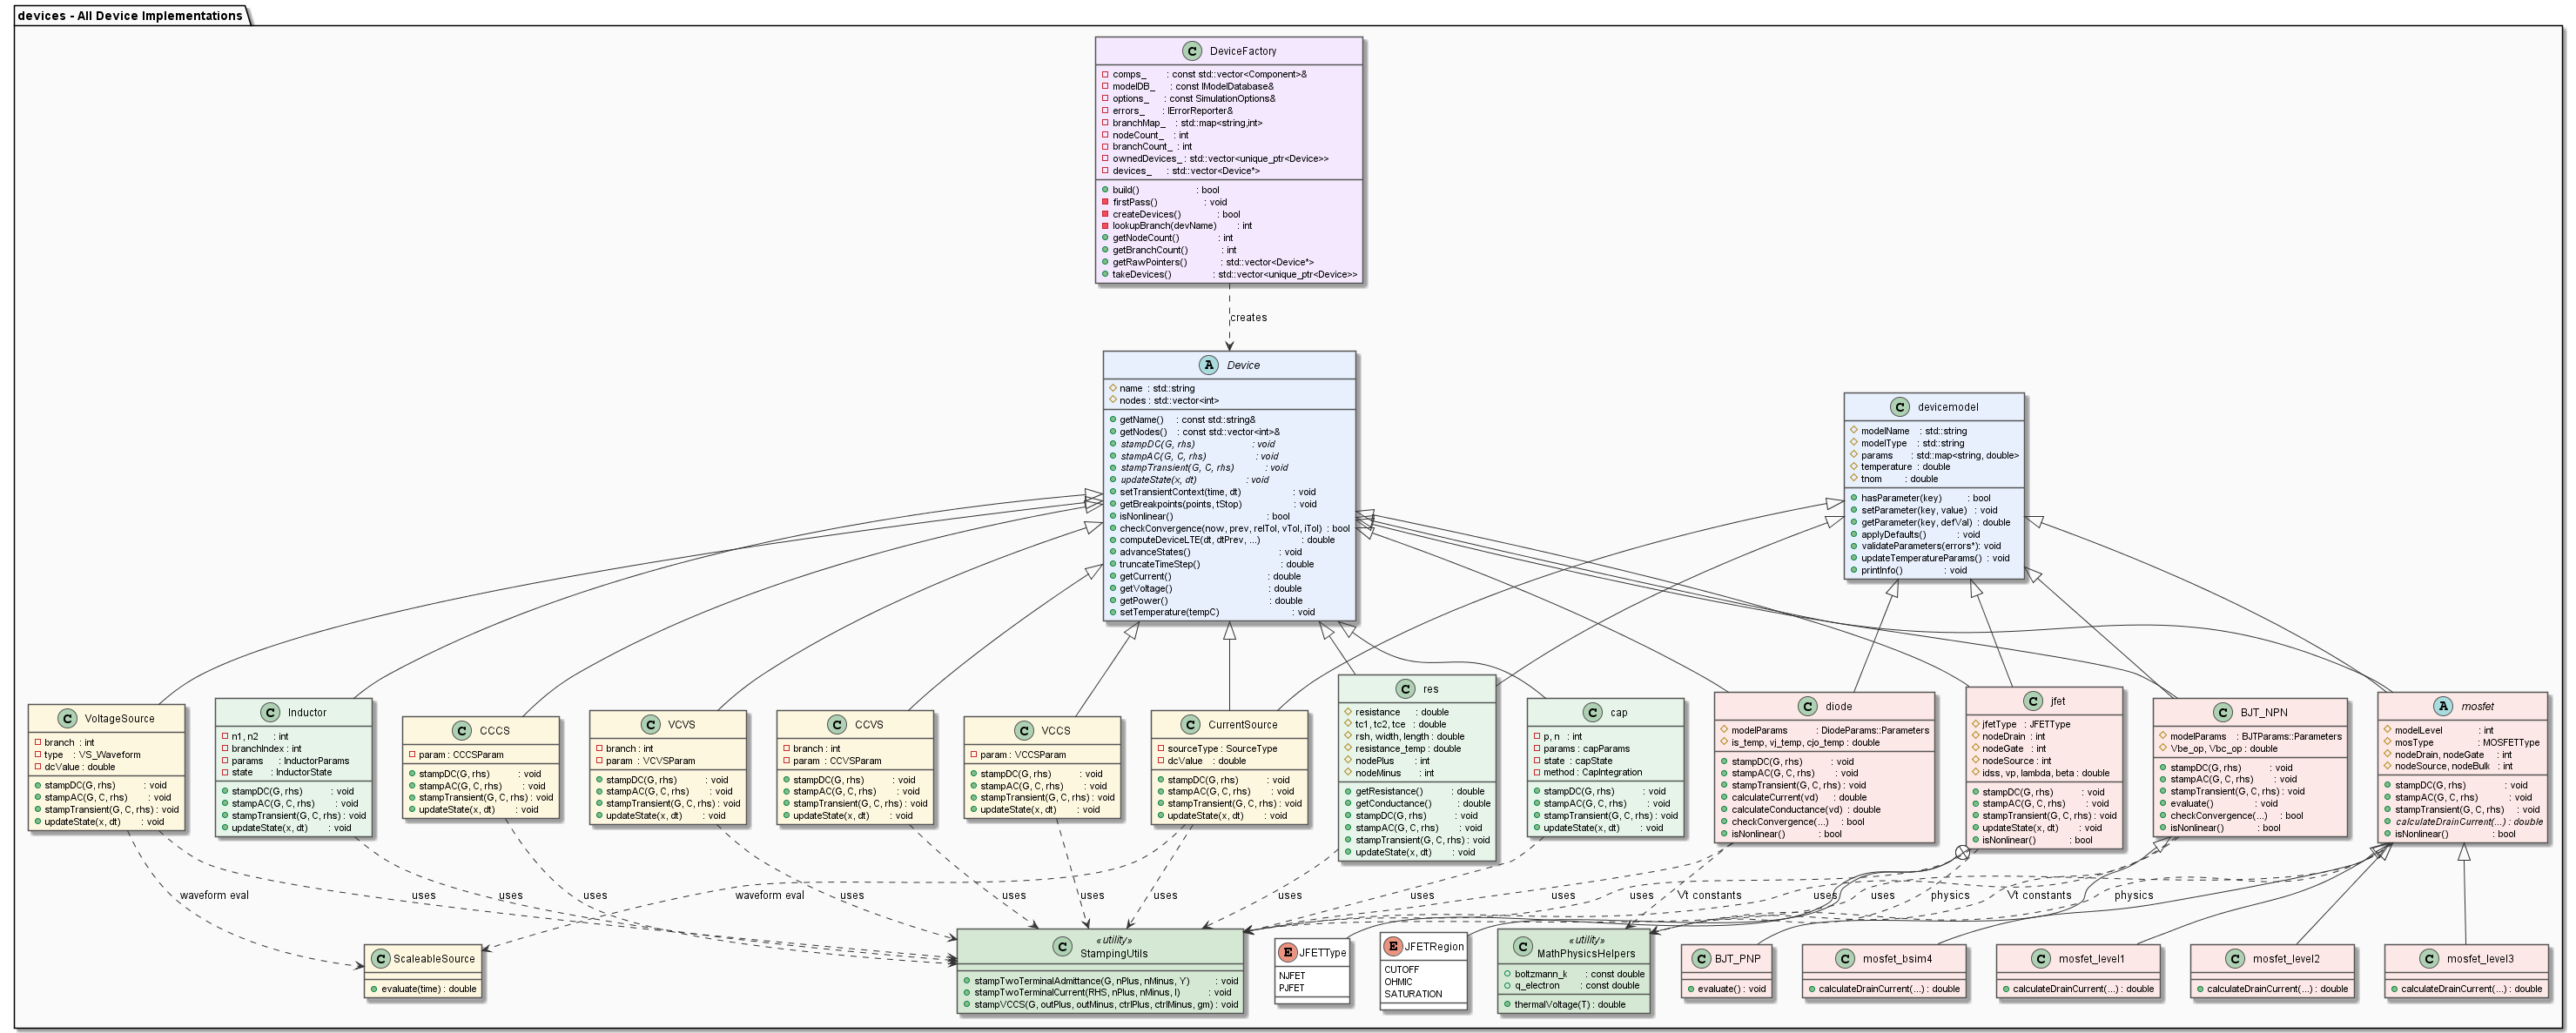
\includegraphics[width=\textwidth,height=0.9\textheight,keepaspectratio]{Figures/Ch5/Devices_Implementations.png}
    \caption{UML Class Diagram of the Device Implementations.}
    \label{fig:devices_uml}
\end{sidewaysfigure}

\begin{figure}[H]
    \centering
    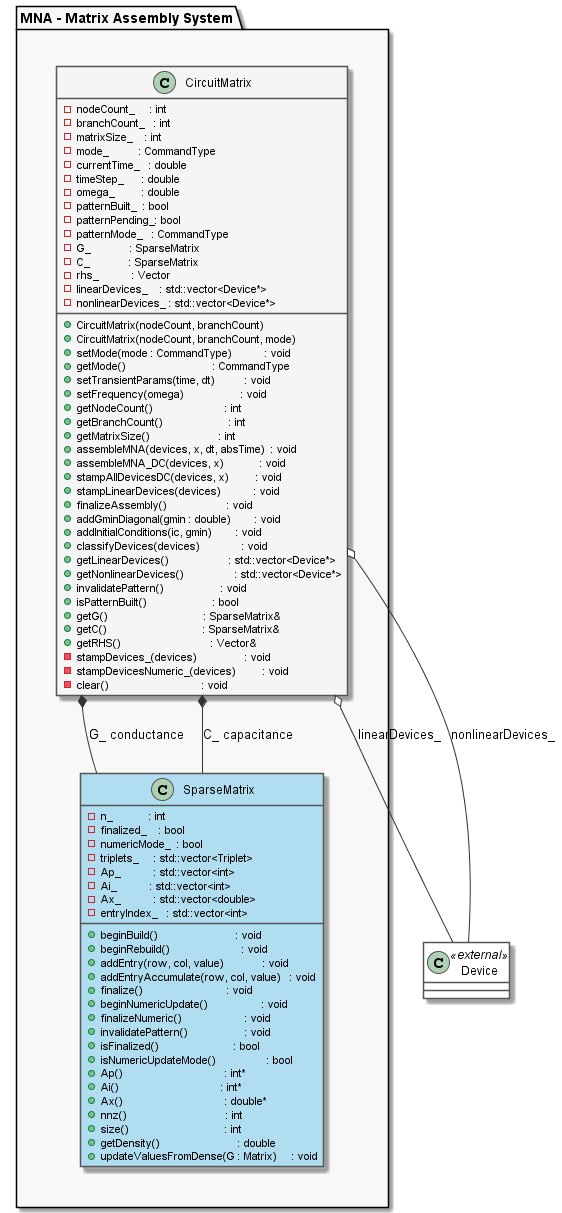
\includegraphics[width=\textwidth,height=0.85\textheight,keepaspectratio]{Figures/Ch5/MNA_Matrix_Assembly_System.png}
    \caption{UML Class Diagram of the MNA Matrix Assembly System.}
    \label{fig:mna_uml}
\end{figure}

\section{Devices}
This section details the mathematical models and software implementation of the supported circuit components. Each device is encapsulated in a class that inherits from a common \texttt{Device} interface, ensuring a consistent API for the simulation engine. To follow an educational progression, the devices are grouped into passive elements, active elements, and sources.

\subsection{Resistor}
The linear resistor is a fundamental passive component in circuit simulation. Its mathematical model is governed by Ohm's law, where the current through the resistor is proportional to the voltage across it, $I = G \cdot V$, with $G = 1/R$ being the conductance.

\subsubsection{Device Model}
The resistor model supports nominal resistance values, temperature dependence, and geometry-based resistance calculations. The temperature-dependent resistance $R(T)$ is modeled using either a polynomial or an exponential formulation based on the given coefficients:
\begin{equation}
    R(T) = R_{\text{nom}} \left[ 1 + TC_1 (T - T_{\text{nom}}) + TC_2 (T - T_{\text{nom}})^2 \right]
\end{equation}
Alternatively, using an exponential coefficient:
\begin{equation}
    R(T) = R_{\text{nom}} \exp\left( TCE (T - T_{\text{nom}}) \right)
\end{equation}
For semiconductor resistors, the resistance can be derived from the sheet resistance $R_{SH}$, width $W$, and length $L$:
\begin{equation}
    R = R_{SH} \frac{L}{W}
\end{equation}

\subsubsection{Software Implementation}
The resistor is implemented in the \texttt{res} class, which inherits from both \texttt{Device} and \texttt{devicemodel}. It maintains parameters such as \texttt{resistance}, temperature coefficients (\texttt{tc1}, \texttt{tc2}, \texttt{tce}), and geometric properties (\texttt{width}, \texttt{length}, \texttt{rsh}).

Since a linear resistor is memoryless and lacks parasitic capacitance in this ideal model, its contribution to the system equations is identical across DC, AC, and Transient analyses. The \texttt{stampConductance} method encapsulates the logic for adding the conductance $g = 1/R(T)$ to the $G$ matrix of the MNA system. For a resistor connected between nodes $n+$ and $n-$, the conductance is added to the diagonal entries $(n+, n+)$ and $(n-, n-)$, and subtracted from the off-diagonal entries $(n+, n-)$ and $(n-, n+)$.

\subsubsection{Workflow and Flowchart}
The workflow of the resistor component involves instantiation, parameter resolution, temperature scaling, and matrix stamping. Figure~\ref{fig:res_flowchart} depicts the execution flow during the simulation setup and analysis phases.

\begin{figure}[H]
    \centering
    \begin{tikzpicture}[node distance=1.5cm,
        box/.style={rectangle, draw, rounded corners, align=center, minimum width=3cm, minimum height=1cm},
        arrow/.style={thick,->,>=stealth}]
        
        \node[box] (init) {Constructor: Initialize nodes and nominal R};
        \node[box, below=0.6cm of init] (defaults) {Apply Defaults: Geometry, TC1, TC2};
        \node[box, below=0.6cm of defaults] (temp) {Update Temperature Params: Compute R(T)};
        \node[box, below=0.6cm of temp] (conductance) {Calculate Conductance: G = 1/R(T)};
        \node[box, below=0.6cm of conductance] (stamp) {MNA Stamping: Add G to SparseMatrix G};
        
        \draw[arrow] (init) -- (defaults);
        \draw[arrow] (defaults) -- (temp);
        \draw[arrow] (temp) -- (conductance);
        \draw[arrow] (conductance) -- (stamp);
        
    \end{tikzpicture}
    \caption{Workflow and Matrix Stamping Flowchart for the Resistor.}
    \label{fig:res_flowchart}
\end{figure}

\subsection{Capacitor}
The capacitor is a fundamental reactive component in circuit simulation. Unlike the linear resistor, its behavior is time-dependent and it introduces memory to the circuit model. The fundamental relationship is $I = \frac{dQ}{dt}$, where $Q$ is the charge stored in the capacitor, which can be a linear or non-linear function of the voltage $V$ across it.

\subsubsection{Device Model}
The implemented capacitor model supports temperature dependence, parasitics (Equivalent Series Resistance, ESR, and minimum conductance leakage, $g_{min}$), and multiple charge-voltage modeling options. The temperature-scaled nominal capacitance is computed as:
\begin{equation}
    C(T) = C_{\text{nom}} \left[ 1 + TC_1 (T - T_{\text{nom}}) + TC_2 (T - T_{\text{nom}})^2 \right]
\end{equation}

Depending on the underlying physics or user specifications, the model can behave as:
\begin{itemize}
    \item \textbf{Ideal}: A standard linear capacitor where $Q(V) = C(T) \cdot V$.
    \item \textbf{Polynomial}: A voltage-dependent capacitor where the charge is given by a polynomial expansion:
    \begin{equation}
        Q(V) = C(T) \cdot V + \frac{1}{2} C_1 V^2 + \frac{1}{3} C_2 V^3
    \end{equation}
    The effective capacitance becomes $C_{\text{eff}} = \frac{dQ}{dV} = C(T) + C_1 V + C_2 V^2$.
    \item \textbf{Varactor}: A junction capacitance model common in semiconductor diodes:
    \begin{equation}
        Q(V) = \frac{C_j V_j}{1 - M} \left[ \left(1 - \frac{V}{V_j}\right)^{1 - M} - 1 \right]
    \end{equation}
    Where $C_j$ is the junction capacitance, $V_j$ is the built-in potential, and $M$ is the grading coefficient.
\end{itemize}

\subsubsection{Software Implementation}
The capacitor is implemented using the \texttt{cap} class, parameterized by \texttt{capParams} and retaining history via the \texttt{capState} structure. This state object maintains values such as $v_{\text{prev}}$, $q_{\text{prev}}$, and $i_{\text{prev}}$, which are crucial for transient analysis numerical integration methods.

During the matrix assembly phase, the capacitor behaves differently depending on the analysis type:
\begin{itemize}
    \item \textbf{DC Analysis}: Since an ideal capacitor behaves as an open circuit under DC steady-state conditions, only its parasitics (such as $1/ESR$ and $g_{min}$) are stamped into the $G$ matrix.
    \item \textbf{AC Analysis}: The linearized effective capacitance around the DC operating point $C_{\text{eff}}(0)$ is stamped into the $C$ matrix (the dynamic matrix), while resistive parasitics are stamped into the $G$ matrix.
    \item \textbf{Transient Analysis}: The effective capacitance at the previous iteration's voltage $C_{\text{eff}}(v_{\text{prev}})$ is evaluated. The admittance equivalent of the reactive component is stamped into the $C$ matrix, while parasitics are integrated into the $G$ matrix. After each integration step, \texttt{updateState} computes the new charge, current, and energy parameters $E = \frac{1}{2} C_{\text{eff}} V^2$ to be used in the next timestep.
\end{itemize}

\subsubsection{Workflow and Flowchart}
The dynamic nature of the capacitor necessitates distinct workflows across simulation modes. Figure~\ref{fig:cap_flowchart} delineates the state initialization and the context-sensitive matrix stamping process.

\begin{figure}[H]
    \centering
    \begin{tikzpicture}[node distance=1.5cm,
        box/.style={rectangle, draw, rounded corners, align=center, minimum width=3cm, minimum height=1cm},
        decision/.style={diamond, draw, align=center, aspect=2},
        arrow/.style={thick,->,>=stealth}]
        
        \node[box] (init) {Initialize Nodes, Parameters (ESR, Model)};
        \node[box, below=0.6cm of init] (temp) {Compute Temperature Scaled C(T)};
        \node[decision, below=0.7cm of temp] (analysis) {Analysis Type?};
        
        \node[box, left=1.8cm of analysis] (dc) {DC Analysis};
        \node[box, below=0.5cm of dc] (dcstamp) {Stamp ESR to G};
        
        \node[box, right=1.8cm of analysis] (ac) {AC Analysis};
        \node[box, below=0.5cm of ac] (acstamp) {Stamp $C_{eff}(0)$ to C\\Stamp ESR to G};
        
        \node[box, below=1.2cm of analysis] (tran) {Transient Analysis};
        \node[box, below=0.5cm of tran] (tran_calc) {Get $v_{prev}$, compute $C_{eff}(v_{prev})$};
        \node[box, below=0.5cm of tran_calc] (transtamp) {Stamp $C_{eff}$ to C\\Stamp ESR/gmin to G};
        \node[box, below=0.5cm of transtamp] (update) {Update State: $v$, $q$, $i$, Energy};
        
        \draw[arrow] (init) -- (temp);
        \draw[arrow] (temp) -- (analysis);
        
        \draw[arrow] (analysis) -- node[above] {DC} (dc);
        \draw[arrow] (dc) -- (dcstamp);
        
        \draw[arrow] (analysis) -- node[above] {AC} (ac);
        \draw[arrow] (ac) -- (acstamp);
        
        \draw[arrow] (analysis) -- node[right] {TRAN} (tran);
        \draw[arrow] (tran) -- (tran_calc);
        \draw[arrow] (tran_calc) -- (transtamp);
        \draw[arrow] (transtamp) -- (update);
        
    \end{tikzpicture}
    \caption{Workflow and Analysis-Dependent Matrix Stamping for the Capacitor.}
    \label{fig:cap_flowchart}
\end{figure}

\subsection{Inductor}
The inductor is a fundamental passive reactive component in circuit simulation. Like the capacitor, its behavior is time-dependent and introduces memory to the circuit equations.

\subsubsection{Device Model}
The voltage-current relationship of an ideal inductor is governed by Faraday's law of induction:
\begin{equation}
    V(t) = L \frac{d I_L}{dt}
\end{equation}
where $L$ is the inductance and $I_L$ is the branch current flowing through the inductor.
The implemented inductor model supports area scaling, temperature dependence, series parasitic resistance ($R_s$), and parallel leakage resistance ($R_p$). The temperature-scaled effective inductance $L(T)$ is computed as:
\begin{equation}
    L(T) = L_{\text{nom}} \cdot \text{Area} \cdot \left[ 1 + TC_1 (T - T_{\text{nom}}) + TC_2 (T - T_{\text{nom}})^2 \right]
\end{equation}
The parallel leakage resistance $R_p$ introduces a path for leakage currents, modeled as a parallel conductance $G_p = 1/R_p$ directly between the nodes:
\begin{equation}
    I_{R_p} = G_p \cdot V
\end{equation}
Under standard Modified Nodal Analysis (MNA), because the current through an ideal inductor cannot be expressed as a simple function of node voltages, the inductor branch current $I_L$ is introduced as an auxiliary branch variable. The branch equation is:
\begin{equation}
    V(n+) - V(n-) - R_s I_L - L(T) \frac{d I_L}{dt} = 0
\end{equation}

\subsubsection{Software Implementation}
The inductor is implemented in the \texttt{Inductor} class, utilizing the \texttt{InductorParams} and \texttt{InductorState} structures.
During the matrix assembly phase, the inductor stamps the system equations:
\begin{itemize}
    \item \textbf{DC Analysis}: The inductor is treated as a short circuit in series with $R_s$. G-matrix stamps place $+1$ and $-1$ at the intersections of the terminals and the branch row/column, and $-R_s$ is stamped at the branch diagonal index.
    \item \textbf{AC Analysis}: Stamps the static topology and parasitic resistances in the $G$ matrix, and stamps the inductance $-L(T)$ in the dynamic $C$ matrix at the branch diagonal position, representing the frequency-dependent impedance $j \omega L(T) + R_s$.
    \item \textbf{Transient Analysis}: The same structural stamping is performed as in AC analysis. The transient solver uses numerical integration (e.g., Backward Euler or Trapezoidal) to assemble the companion model. For Backward Euler, the system becomes $(G + C/\Delta t) \cdot x^{[n+1]} = RHS + C/\Delta t \cdot x^{[n]}$, where the history term is managed by the solver.
\end{itemize}

\subsubsection{Workflow and Flowchart}
Figure~\ref{fig:ind_flowchart} shows the execution flow for the inductor, highlighting the parameter resolution, temperature scaling, and analysis-dependent matrix stamping.

\begin{figure}[H]
    \centering
    \begin{tikzpicture}[node distance=1.5cm,
        box/.style={rectangle, draw, rounded corners, align=center, minimum width=3.5cm, minimum height=1cm},
        decision/.style={diamond, draw, align=center, aspect=2, inner sep=0pt},
        arrow/.style={thick,->,>=stealth}]
        
        \node[box] (init) {Initialize Nodes, Branch Current Index};
        \node[box, below=0.6cm of init] (temp) {Evaluate $L(T)$ via Area \\ and Temperature TC1, TC2};
        \node[decision, below=0.7cm of temp] (analysis) {Analysis Type?};
        
        \node[box, left=1.8cm of analysis] (dc) {DC Analysis};
        \node[box, below=0.5cm of dc] (dcstamp) {Stamp topology in $G$\\Stamp $R_s$ and $R_p$ (conductance)};
        
        \node[box, right=1.8cm of analysis] (ac) {AC Analysis};
        \node[box, below=0.5cm of ac] (acstamp) {Stamp topology and Rs/Rp in $G$\\Stamp $-L(T)$ in $C$};
        
        \node[box, below=1.2cm of analysis] (tran) {Transient Analysis};
        \node[box, below=0.5cm of tran] (transtamp) {Stamp topology and Rs/Rp in $G$\\Stamp $-L(T)$ in $C$};
        \node[box, below=0.5cm of transtamp] (update) {Update State: Read $I_L$ and $V_L$ \\ from Solution Vector};
        
        \draw[arrow] (init) -- (temp);
        \draw[arrow] (temp) -- (analysis);
        
        \draw[arrow] (analysis) -- node[above] {DC} (dc);
        \draw[arrow] (dc) -- (dcstamp);
        
        \draw[arrow] (analysis) -- node[above] {AC} (ac);
        \draw[arrow] (ac) -- (acstamp);
        
        \draw[arrow] (analysis) -- node[right] {TRAN} (tran);
        \draw[arrow] (tran) -- (transtamp);
        \draw[arrow] (transtamp) -- (update);
        
    \end{tikzpicture}
    \caption{Workflow and Analysis-Dependent Matrix Stamping for the Inductor.}
    \label{fig:ind_flowchart}
\end{figure}

\subsection{Diode}
The diode is a non-linear two-terminal semiconductor device that allows current to flow primarily in one direction. Its mathematical modeling is critical for capturing rectification, clamping, and switching behaviors.

\subsubsection{Device Model}
The model is based on the Shockley diode equation, extended with temperature scaling, reverse breakdown physics, and dynamic junction capacitances. The DC current $I_D$ is expressed as:
\begin{equation}
    I_D = I_S \left( e^{\frac{V_D}{n V_t}} - 1 \right) - I_{BV} e^{-\frac{V_D + B_V}{V_t}}
\end{equation}
where $I_S$ is the saturation current, $n$ is the emission coefficient, $V_t = k T / q$ is the thermal voltage, $B_V$ is the breakdown voltage, and $I_{BV}$ is the current at breakdown.
The dynamic behavior is modeled by the charge $Q_D$, which consists of diffusion charge (due to transit time $\tau_D$) and depletion charge:
\begin{equation}
    Q_D = \tau_D \cdot I_D + Q_j(V_D)
\end{equation}
The junction capacitance $C_j(V_D) = d Q_j / d V_D$ is modeled as:
\begin{equation}
    C_j(V_D) = \begin{cases}
        \frac{C_{j0}}{\left( 1 - \frac{V_D}{V_j} \right)^M} & V_D < FC \cdot V_j \\
        \frac{C_{j0}}{(1 - FC)^{1+M}} \left[ 1 - FC(1+M) + M \frac{V_D}{V_j} \right] & V_D \ge FC \cdot V_j
    \end{cases}
\end{equation}

\subsubsection{Software Implementation}
The diode is implemented in the \texttt{diode} class. In order to handle the non-linear equation, the Newton-Raphson solver linearizes the device at each iteration. The Taylor series expansion of $I_D(V_D)$ yields:
\begin{equation}
    I_D(V_D^{(k+1)}) \approx I_D(V_D^{(k)}) + g_d \left( V_D^{(k+1)} - V_D^{(k)} \right)
\end{equation}
where $g_d = d I_D / d V_D$ is the small-signal conductance. The linearized companion model consists of a parallel conductance $g_d$ and a Norton equivalent current source:
\begin{equation}
    I_{eq} = I_D(V_D^{(k)}) - g_d \cdot V_D^{(k)}
\end{equation}
To prevent exponential overflow during iterations, a voltage-limiting function \texttt{pnjlim} is applied to restrict node voltage updates.
The device stamps the MNA system as follows:
\begin{itemize}
    \item \textbf{G Matrix}: Stamps $g_d$ (along with optional series resistance $r_s$ and minimum conductance $g_{\text{min}}$) between the anode, cathode, and internal anode prime nodes.
    \item \textbf{C Matrix}: Stamps the total capacitance $C_D = \tau_D g_d + C_j(V_D)$ for AC and transient analysis.
    \item \textbf{RHS Vector}: Stamps the equivalent current $I_{eq}$ to drive the Newton-Raphson iterations.
\end{itemize}
Self-heating is supported through an optional thermal node and thermal impedance parameters.

\subsubsection{Workflow and Flowchart}
Figure~\ref{fig:diode_flowchart} outlines the evaluation and stamping cycle for the Diode model during iterative simulation.

\begin{figure}[H]
    \centering
    \begin{tikzpicture}[node distance=1.5cm,
        box/.style={rectangle, draw, rounded corners, align=center, minimum width=3.5cm, minimum height=1cm},
        decision/.style={diamond, draw, align=center, aspect=2, inner sep=0pt},
        arrow/.style={thick,->,>=stealth}]
        
        \node[box] (voltages) {Get Nodal Voltages: $V_a, V_c$};
        \node[box, below=0.6cm of voltages] (lim) {Apply \texttt{pnjlim} to prevent exponential overflow};
        \node[box, below=0.6cm of lim] (eval) {Evaluate Current $I_D$ and Conductance $g_d$};
        \node[box, below=0.6cm of eval] (caps) {Compute Diffusion and Depletion Capacitances};
        \node[decision, below=0.7cm of caps] (analysis) {Analysis Type?};
        
        \node[box, left=1.8cm of analysis] (dc) {DC / TRAN};
        \node[box, below=0.5cm of dc] (dcstamp) {Stamp $g_d$ in $G$\\Stamp $I_{eq}$ in RHS};
        
        \node[box, right=1.8cm of analysis] (ac) {AC Analysis};
        \node[box, below=0.5cm of ac] (acstamp) {Stamp $g_d$ in $G$\\Stamp $C_D$ in $C$};
        
        \node[box, below=1.2cm of dcstamp] (tran_add) {If TRAN: \\Stamp $C_D$ in $C$\\Compute transient RHS companion};
        
        \draw[arrow] (voltages) -- (lim);
        \draw[arrow] (lim) -- (eval);
        \draw[arrow] (eval) -- (caps);
        \draw[arrow] (caps) -- (analysis);
        
        \draw[arrow] (analysis) -- node[above] {DC/TRAN} (dc);
        \draw[arrow] (dc) -- (dcstamp);
        \draw[arrow] (dcstamp) -- (tran_add);
        
        \draw[arrow] (analysis) -- node[above] {AC} (ac);
        \draw[arrow] (ac) -- (acstamp);
        
    \end{tikzpicture}
    \caption{Workflow and Newton-Raphson Stamping Flow for the Diode.}
    \label{fig:diode_flowchart}
\end{figure}

\subsection{Junction Field-Effect Transistor (JFET)}
The Junction Field-Effect Transistor (JFET) is a three-terminal semiconductor device that relies on an electric field to control the conductivity of a channel. Unlike MOSFETs, the JFET gate is formed by a reverse-biased PN junction rather than an insulating oxide layer. Consequently, the device is normally-on (depletion mode) and allows current to flow when the gate-source voltage is zero. 

\subsubsection{Device Model}
The implemented mathematical model is based on the Shockley square-law (Level 1) representation, extended with channel-length modulation, temperature scaling, and non-linear junction capacitances. The model accommodates both N-channel and P-channel JFETs, with the primary distinction being the polarity of the pinch-off voltage ($V_p < 0$ for N-JFET) and the direction of drain current $I_d$. 

The core DC characteristics are determined by the operating region:
\begin{itemize}
    \item \textbf{Cutoff}: When $|V_{gs}| \ge |V_p|$, the channel is fully depleted, and $I_d \approx 0$.
    \item \textbf{Ohmic (Linear)}: When $|V_{ds}| < |V_{gs} - V_p|$, the device acts as a voltage-controlled resistor:
    \begin{equation}
        I_d = \frac{I_{dss}}{V_p^2} \left[ 2(V_{gs}-V_p)V_{ds} - V_{ds}^2 \right] (1 + \lambda V_{ds})
    \end{equation}
    \item \textbf{Saturation (Active)}: When $|V_{ds}| \ge |V_{gs} - V_p|$, the current saturates and becomes primarily dependent on $V_{gs}$:
    \begin{equation}
        I_d = I_{dss} \left( 1 - \frac{V_{gs}}{V_p} \right)^2 (1 + \lambda V_{ds})
    \end{equation}
\end{itemize}
where $I_{dss}$ is the maximum saturation current (at $V_{gs}=0$), $V_p$ is the pinch-off voltage, and $\lambda$ models the channel-length modulation. Alternatively, process parameters can define these values via $I_{dss} = \beta V_{to}^2$ and $V_p = V_{to}$.

Temperature scaling plays a critical role in the JFET model. The saturation current scales as $I_{dss}(T) = I_{dss} (T/T_{\text{nom}})^{-1.5}$, while the pinch-off voltage undergoes a linear shift (approximately $+2.5 \text{ mV}/^\circ\text{C}$). Additionally, the model considers the reverse leakage current of the gate junction, governed by $I_S(T) = I_S (T/T_{\text{nom}})^3$.

The dynamic behavior is modeled by voltage-dependent gate-source ($C_{gs}$) and gate-drain ($C_{gd}$) junction capacitances, computed based on the built-in potential $PB$ and a grading coefficient.

\subsubsection{Software Implementation}
The JFET is encapsulated within the \texttt{jfet} class. Due to the device's highly non-linear nature, simulation requires iterative solvers such as the Newton-Raphson method. During each iteration, the \texttt{updateState} method calculates the operating point (OP) parameters based on the latest nodal voltages:
\begin{itemize}
    \item Large-signal currents: $I_d$, $I_{gs}$, $I_{gd}$.
    \item Small-signal conductances: $g_m = \frac{\partial I_d}{\partial V_{gs}}$, $g_{ds} = \frac{\partial I_d}{\partial V_{ds}}$, $g_{gs} = \frac{\partial I_{gs}}{\partial V_{gs}}$, $g_{gd} = \frac{\partial I_{gd}}{\partial V_{gd}}$.
    \item Dynamic capacitances: $C_{gs}$, $C_{gd}$, and the constant parasitic $C_{ds}$.
\end{itemize}

The matrix assembly integrates these OP parameters. The device is transformed into a linear companion model consisting of linear conductances ($g_{ds}$, $g_{gs}$, $g_{gd}$), a voltage-controlled current source ($g_m \cdot V_{gs}$), and Norton equivalent independent current sources ($I_{eq}$) that account for the non-linear residual currents. 
\begin{itemize}
    \item \textbf{G Matrix}: Stamps the linear conductances $g_{ds}, g_{gs}, g_{gd}$ and the transconductance $g_m$ (which links the drain and source equations via the gate control voltage).
    \item \textbf{C Matrix}: Stamps the dynamic junction capacitances $C_{gs}, C_{gd}$, and the parasitic $C_{ds}$ for AC and Transient analyses.
    \item \textbf{RHS Vector}: Stamps the Norton equivalent currents ($I_{eq\_d}$, $I_{eq\_gs}$, $I_{eq\_gd}$) into the Right-Hand Side vector to drive the Newton-Raphson iterations.
\end{itemize}

\subsubsection{Workflow and Flowchart}
The JFET simulation workflow is inherently tied to the iterative non-linear solver. Figure~\ref{fig:jfet_flowchart} depicts the sequence of evaluating the operating point and stamping the companion model into the system matrices.

\begin{figure}[H]
    \centering
    \begin{tikzpicture}[node distance=1.5cm,
        box/.style={rectangle, draw, rounded corners, align=center, minimum width=3cm, minimum height=1cm},
        decision/.style={diamond, draw, align=center, aspect=2, inner sep=0pt},
        arrow/.style={thick,->,>=stealth}]
        
        \node[box] (voltages) {Get Nodal Voltages $X$: Compute $V_{gs}, V_{ds}, V_{gd}$};
        \node[box, below=0.6cm of voltages] (op) {Update OP: Evaluate $I_d, g_m, g_{ds}$, Caps};
        \node[decision, below=0.6cm of op] (analysis) {Analysis?};
        
        \node[box, left=1.8cm of analysis] (dc) {DC / TRAN};
        \node[box, below=0.5cm of dc] (dcstamp) {Stamp $G$ (Conductances)\\Stamp RHS (Norton $I_{eq}$)};
        
        \node[box, right=1.8cm of analysis] (ac) {AC Analysis};
        \node[box, below=0.5cm of ac] (acstamp) {Stamp $G$ (Conductances)\\Stamp $C$ (Capacitances)};
        
        \node[box, below=1.2cm of dcstamp] (tran_add) {If TRAN: \\Stamp $C$ Matrix};
        
        \draw[arrow] (voltages) -- (op);
        \draw[arrow] (op) -- (analysis);
        
        \draw[arrow] (analysis) -- node[above] {DC/TRAN} (dc);
        \draw[arrow] (dc) -- (dcstamp);
        \draw[arrow] (dcstamp) -- (tran_add);
        
        \draw[arrow] (analysis) -- node[above] {AC} (ac);
        \draw[arrow] (ac) -- (acstamp);
        
    \end{tikzpicture}
    \caption{Workflow and Analysis-Dependent Matrix Stamping for the Non-linear JFET.}
    \label{fig:jfet_flowchart}
\end{figure}

\subsection{Metal-Oxide-Semiconductor Field-Effect Transistor (MOSFET)}
The MOSFET is the most critical four-terminal (Drain, Gate, Source, Bulk) semiconductor device in modern integrated circuit design. Its highly non-linear nature and reliance on complex physical phenomena make its mathematical modeling and software implementation the most intensive part of the simulation engine.

\subsubsection{Device Model}
The implemented architecture supports a hierarchy of model levels to balance computational speed with physical accuracy:
\begin{itemize}
    \item \textbf{Level 1 (Shichman-Hodges)}: The foundational square-law model. It provides basic Cutoff, Linear, and Saturation region equations, accounting for channel-length modulation ($\lambda$) and the body effect ($\gamma$).
    \item \textbf{Level 2 \& 3}: Advanced analytical and semi-empirical models that incorporate short-channel effects, such as velocity saturation, mobility degradation, and Drain-Induced Barrier Lowering (DIBL).
    \item \textbf{Level 54 (BSIM4 Core)}: The industry standard for deep-submicron designs, accommodating complex geometry dependencies and advanced threshold voltage roll-off physics.
\end{itemize}

Beyond the core channel current, the model implements a comprehensive suite of parasitic elements. This includes the non-linear bulk-source and bulk-drain junction diodes (incorporating reverse breakdown physics) and voltage-dependent overlap and junction capacitances. Furthermore, terminal charges ($Q_g$, $Q_d$, $Q_s$, $Q_b$) are evaluated using the charge-conserving Ward-Dutton partition model.

\subsubsection{Software Implementation}
The \texttt{mosfet} base class establishes the common interface for all model levels. Since the MOSFET characteristics are strongly non-linear, the component heavily relies on the Newton-Raphson (NR) iterative solver. 

During each NR iteration, the \texttt{updateOperatingPoint} function extracts the effective terminal voltages ($V_{gs}$, $V_{ds}$, $V_{bs}$) and calculates the required small-signal parameters. To maintain architectural flexibility and simplify the implementation of complex models like BSIM4, parameters such as $g_m$, $g_{ds}$, and $g_{mb}$ are obtained via robust symmetric finite difference numerical differentiation. Additionally, a \texttt{fetlimit} algorithm restricts voltage jumps between consecutive iterations to prevent numerical overflow in exponential regions.

The MNA stamping translates the non-linear device into a linear companion model:
\begin{itemize}
    \item \textbf{G Matrix}: Stamps the output conductance ($g_{ds}$) between drain and source, alongside voltage-controlled current sources representing the main transconductance ($g_m \cdot V_{gs}$) and the bulk transconductance ($g_{mb} \cdot V_{bs}$). It also stamps the body diode conductances ($g_{bs}$, $g_{bd}$).
    \item \textbf{C Matrix}: Stamps the voltage-dependent capacitances ($C_{gs}$, $C_{gd}$, $C_{gb}$, $C_{bs}$, $C_{bd}$) for AC and transient integration.
    \item \textbf{RHS Vector}: Injects the Norton equivalent currents ($I_{eq}$) that offset the linearised conductances back to the true non-linear operating point.
\end{itemize}

\subsubsection{Workflow and Flowchart}
Figure~\ref{fig:mosfet_flowchart} outlines the extensive internal evaluation cycle required to linearise and stamp the MOSFET during a single non-linear solver iteration.

\begin{figure}[H]
    \centering
    \begin{tikzpicture}[node distance=1.5cm,
        box/.style={rectangle, draw, rounded corners, align=center, minimum width=3.5cm, minimum height=1cm},
        decision/.style={diamond, draw, align=center, aspect=2, inner sep=0pt},
        arrow/.style={thick,->,>=stealth}]
        
        \node[box] (voltages) {Get Nodal Voltages $V_d, V_g, V_s, V_b$ \\ Apply \texttt{fetlimit} bounds};
        \node[box, below=0.6cm of voltages] (op) {Evaluate OP: $I_d$, $g_m$, $g_{ds}$, $g_{mb}$ \\ via Model Level Equations};
        \node[box, below=0.6cm of op] (parasitics) {Evaluate Ward-Dutton Charges, \\ Capacitances, and Body Diodes};
        \node[decision, below=0.6cm of parasitics] (analysis) {Analysis?};
        
        \node[box, left=1.8cm of analysis] (dc) {DC / TRAN};
        \node[box, below=0.5cm of dc] (dcstamp) {Stamp $G$ ($g_{ds}, g_m, g_{mb}$, Diodes)\\Stamp RHS (Norton $I_{eq}$)};
        
        \node[box, right=1.8cm of analysis] (ac) {AC Analysis};
        \node[box, below=0.5cm of ac] (acstamp) {Stamp $G$ (Conductances)\\Stamp $C$ (Capacitances)};
        
        \node[box, below=1.2cm of dcstamp] (tran_add) {If TRAN: \\Stamp $C$ Matrix \\ Compute Integration RHS};
        
        \draw[arrow] (voltages) -- (op);
        \draw[arrow] (op) -- (parasitics);
        \draw[arrow] (parasitics) -- (analysis);
        
        \draw[arrow] (analysis) -- node[above] {DC/TRAN} (dc);
        \draw[arrow] (dc) -- (dcstamp);
        \draw[arrow] (dcstamp) -- (tran_add);
        
        \draw[arrow] (analysis) -- node[above] {AC} (ac);
        \draw[arrow] (ac) -- (acstamp);
        
    \end{tikzpicture}
    \caption{Workflow and Matrix Stamping for the Multi-Level MOSFET Model.}
    \label{fig:mosfet_flowchart}
\end{figure}

\subsection{Bipolar Junction Transistor (BJT)}
The Bipolar Junction Transistor (BJT) is a four-terminal (Collector, Base, Emitter, Substrate) active device. Modeling BJTs accurately is critical for amplifiers and high-speed circuit designs.

\subsubsection{Device Model}
The implementation is based on the Ebers-Moll transport model, incorporating the Early effect (forward and reverse Early voltages $V_{af}, V_{ar}$), high-current beta roll-off ($IKF$), temperature scaling, base resistance modulation, and substrate junction leakage.
The principal transport current $I_{tr}$ flowing from collector to emitter is governed by:
\begin{equation}
    I_{tr} = \frac{I_f - I_r}{q_b}
\end{equation}
where $I_f$ and $I_r$ are the forward and reverse junction transport currents:
\begin{equation}
    I_f = I_S \left( e^{\frac{V_{be}}{N_f V_t}} - 1 \right), \quad I_r = I_S \left( e^{\frac{V_{bc}}{N_r V_t}} - 1 \right)
\end{equation}
and $q_b$ is the normalized base charge modeling the Early effect and high-current injection:
\begin{equation}
    q_b = \frac{q_1}{2} \left( 1 + \sqrt{1 + 4 q_2} \right)
\end{equation}
with:
\begin{equation}
    q_1 = \left( 1 - \frac{V_{bc}}{V_{af}} - \frac{V_{be}}{V_{ar}} \right)^{-1}, \quad q_2 = \frac{I_f}{I_{kf}} + \frac{I_r}{I_{kr}}
\end{equation}
The base terminal current $I_b$ includes the diode transport currents divided by beta, plus recombination leakage:
\begin{equation}
    I_b = \frac{I_f}{\beta_f} + \frac{I_r}{\beta_r} + I_{se} \left( e^{\frac{V_{be}}{N_e V_t}} - 1 \right) + I_{sc} \left( e^{\frac{V_{bc}}{N_c V_t}} - 1 \right)
\end{equation}

The dynamic behavior is modeled by voltage-dependent capacitances:
\begin{equation}
    C_{be} = C_{je}(V_{be}) + \tau_f g_m, \quad C_{bc} = \text{XCJC} \cdot C_{jc}(V_{bc}) + \tau_r g_{mu}
\end{equation}
Additionally, substrate current $I_{sub}$ and junction capacitance $C_{sub}$ are modeled at the substrate terminal.

\subsubsection{Software Implementation}
The BJT is implemented within the \texttt{BJT\_NPN} and \texttt{BJT\_PNP} classes.
During each Newton-Raphson iteration, the terminal voltages are extracted and junction voltages are limited using `pnjlim`. The \texttt{evaluate} method calculates the currents, small-signal transconductance $g_m$, output conductance $g_o$, junction conductances $g_{\pi}, g_{\mu}$, and dynamic capacitances.
The device stamps the MNA system as follows:
\begin{itemize}
    \item \textbf{G Matrix}: Stamps small-signal parameters $g_{\pi}, g_{\mu}, g_m, g_o$ and parasitic series conductances for base, collector, emitter, and substrate nodes.
    \item \textbf{C Matrix}: Stamps $C_{be}, C_{bc}, C_{sub}$, and the extrinsic collector-base capacitance $C_{bx}$.
    \item \textbf{RHS Vector}: Stamps the Norton equivalent current sources:
    \begin{align}
        I_{eq,be} &= I_{be} - g_{\pi} V_{be} \\
        I_{eq,bc} &= I_{bc} - g_{\mu} V_{bc} \\
        I_{eq,c} &= (I_c + I_{bc}) - g_m V_{be} - g_o V_{ce}
    \end{align}
\end{itemize}

\subsubsection{Workflow and Flowchart}
Figure~\ref{fig:bjt_flowchart} demonstrates the evaluation, limiting, and MNA stamping logic of the BJT model.

\begin{figure}[H]
    \centering
    \begin{tikzpicture}[node distance=1.5cm,
        box/.style={rectangle, draw, rounded corners, align=center, minimum width=3.5cm, minimum height=1cm},
        decision/.style={diamond, draw, align=center, aspect=2, inner sep=0pt},
        arrow/.style={thick,->,>=stealth}]
        
        \node[box] (voltages) {Get Terminal Voltages $V_c, V_b, V_e, V_s$};
        \node[box, below=0.6cm of voltages] (lim) {Apply \texttt{pnjlim} to $V_{be}$ and $V_{bc}$};
        \node[box, below=0.6cm of lim] (eval) {Evaluate Ebers-Moll Currents, \\ Base Charge $q_b$, and Conductances};
        \node[box, below=0.6cm of eval] (caps) {Compute Junction/Diffusion Capacitances};
        \node[decision, below=0.7cm of caps] (analysis) {Analysis Type?};
        
        \node[box, left=1.8cm of analysis] (dc) {DC / TRAN};
        \node[box, below=0.5cm of dc] (dcstamp) {Stamp $G$ with conductances\\Stamp RHS with Norton $I_{eq}$};
        
        \node[box, right=1.8cm of analysis] (ac) {AC Analysis};
        \node[box, below=0.5cm of ac] (acstamp) {Stamp $G$ with conductances\\Stamp $C$ with capacitances};
        
        \node[box, below=1.2cm of dcstamp] (tran_add) {If TRAN: \\Stamp $C$ with capacitances\\Stamp Transient companion sources};
        
        \draw[arrow] (voltages) -- (lim);
        \draw[arrow] (lim) -- (eval);
        \draw[arrow] (eval) -- (caps);
        \draw[arrow] (caps) -- (analysis);
        
        \draw[arrow] (analysis) -- node[above] {DC/TRAN} (dc);
        \draw[arrow] (dc) -- (dcstamp);
        \draw[arrow] (dcstamp) -- (tran_add);
        
        \draw[arrow] (analysis) -- node[above] {AC} (ac);
        \draw[arrow] (ac) -- (acstamp);
        
    \end{tikzpicture}
    \caption{Workflow and Newton-Raphson Stamping Flow for the BJT.}
    \label{fig:bjt_flowchart}
\end{figure}

\subsection{Independent Voltage Source (VS)}
The independent voltage source is a fundamental active component that forces a specific potential difference between two nodes, irrespective of the current drawn. Because its current is an independent variable determined by the rest of the circuit, incorporating a voltage source requires expanding the standard nodal equations.

\subsubsection{Device Model}
The voltage source model supports both steady-state (DC) and time-varying transient waveforms. The supported waveform types mirror the standard SPICE specifications:
\begin{itemize}
    \item \textbf{DC}: A constant DC value.
    \item \textbf{PULSE}: A periodic pulse waveform defined by initial/pulsed values, delay, rise/fall times, pulse width, and period.
    \item \textbf{SIN}: A damped sinusoidal waveform with offset, amplitude, frequency, delay, damping factor, and phase.
    \item \textbf{EXP}: An exponential waveform featuring independent rise and fall time constants.
    \item \textbf{PWL (Piece-Wise Linear)}: An arbitrary waveform constructed by linear interpolation between user-defined $(time, voltage)$ data points.
\end{itemize}

\subsubsection{Software Implementation}
The \texttt{VoltageSource} class implements this behavior. Since nodal analysis normally solves for node voltages using current equations ($Y V = I$), an ideal voltage source cannot be represented by a finite conductance. Thus, Modified Nodal Analysis (MNA) introduces an additional variable (the source current) and an additional constraint equation (the voltage relationship).

The device holds a \texttt{branch} index, representing its assigned extra row and column in the MNA matrices. 
For a source connected between the positive node $p$ and the negative node $n$:
\begin{itemize}
    \item \textbf{G Matrix}: A value of $+1$ is stamped at $(p, \text{branch})$ and $(\text{branch}, p)$. A value of $-1$ is stamped at $(n, \text{branch})$ and $(\text{branch}, n)$. 
    \item \textbf{RHS Vector}: The instantaneous voltage $V(t)$ is stamped into the RHS vector at the index corresponding to the \texttt{branch}.
\end{itemize}

This topological stamping structure is identical across DC, AC, and Transient analyses, with only the RHS value changing (e.g., $V_{\text{DC}}$ for DC, AC amplitude for AC, and $V(t)$ for Transient). After the linear solver executes, \texttt{updateState} retrieves the computed source current from the solution vector at the \texttt{branch} index.

A critical feature of the transient implementation is the \texttt{getBreakpoints} method. To ensure numerical accuracy and prevent the integration engine from stepping over sharp waveform transitions (such as pulse edges or PWL corners), the voltage source reports these critical timestamps to the transient controller, which adjusts its dynamic timestep accordingly.

\subsubsection{Workflow and Flowchart}
Figure~\ref{fig:vs_flowchart} depicts the execution cycle for a voltage source, highlighting the waveform evaluation, MNA branch stamping, and state retrieval phases.

\begin{figure}[H]
    \centering
    \begin{tikzpicture}[node distance=1.5cm,
        box/.style={rectangle, draw, rounded corners, align=center, minimum width=4cm, minimum height=1cm},
        arrow/.style={thick,->,>=stealth}]
        
        \node[box] (init) {Initialize Nodes, Branch Index, and Waveform Params};
        \node[box, below=0.6cm of init] (breaks) {Export Breakpoints to Simulation Engine};
        \node[box, below=0.6cm of breaks] (time) {Simulation Loop: Receive current $time, dt$};
        \node[box, below=0.6cm of time] (eval) {Evaluate $V(t) = \text{evalWaveform}(time)$};
        \node[box, below=0.6cm of eval] (stamp) {MNA Stamping: \\ $G$: $\pm 1$ at branch/node intersections \\ RHS: Stamp $V(t)$ at branch row};
        \node[box, below=0.6cm of stamp] (update) {Update State: Read $I_{\text{source}}$ from $X[\text{branch}]$};
        
        \draw[arrow] (init) -- (breaks);
        \draw[arrow] (breaks) -- (time);
        \draw[arrow] (time) -- (eval);
        \draw[arrow] (eval) -- (stamp);
        \draw[arrow] (stamp) -- (update);
        \draw[arrow, dashed] (update.west) -- ++(-1,0) |- (time.west);
        
    \end{tikzpicture}
    \caption{Workflow, Waveform Evaluation, and MNA Stamping for the Voltage Source.}
    \label{fig:vs_flowchart}
\end{figure}

\subsection{Independent Current Source (CS)}
The independent current source is a foundational active component that injects a prescribed current into a circuit branch, regardless of the voltage developed across its terminals. Unlike voltage sources, ideal current sources do not require the introduction of auxiliary branch variables in the Modified Nodal Analysis (MNA) formulation.

\subsubsection{Device Model}
The current source model provides the same comprehensive suite of SPICE-standard steady-state and transient waveforms as the voltage source:
\begin{itemize}
    \item \textbf{DC}: A steady, constant current injection.
    \item \textbf{PULSE}: A periodic current pulse defined by rise/fall times and pulse width.
    \item \textbf{SIN}: A damped sinusoidal current profile.
    \item \textbf{EXP}: An exponential transient current with independent rise and fall envelopes.
    \item \textbf{PWL (Piece-Wise Linear)}: A custom arbitrary waveform generated from user-supplied $(time, current)$ coordinates.
\end{itemize}

\subsubsection{Software Implementation}
The \texttt{cs} class implements the independent current source. Because the device current is explicitly known from the waveform evaluation, it acts purely as a driving stimulus to the nodal equations ($Y V = I$).

For a current source connected between a positive node $N+$ and a negative node $N-$ (where positive current conventionally exits $N+$ and enters $N-$), the MNA stamping procedure is exceptionally lightweight:
\begin{itemize}
    \item \textbf{G and C Matrices}: No entries are added. An ideal current source has zero admittance (infinite internal resistance).
    \item \textbf{RHS Vector}: The instantaneous current value $I(t)$ is subtracted from the $N+$ row ($RHS[N+] \mathrel{{-}{=}} I(t)$) and added to the $N-$ row ($RHS[N-] \mathrel{{+}{=}} I(t)$).
\end{itemize}

This RHS-only stamping logic remains structurally identical for DC ($I_{\text{DC}}$), AC ($I_{\text{AC}}$), and Transient ($I(t)$) analyses.

Similar to the voltage source, the current source implements the \texttt{getBreakpoints} method. By reporting the timestamps of abrupt changes (such as PULSE edges or PWL vertices) to the simulation engine, it guarantees that the transient integration timestep aligns with the discontinuity, ensuring numerical stability and accuracy.

\subsubsection{Workflow and Flowchart}
Figure~\ref{fig:cs_flowchart} illustrates the straightforward execution cycle of the independent current source. Since no auxiliary states are solved via the MNA matrix, the post-solution state update is trivial.

\begin{figure}[H]
    \centering
    \begin{tikzpicture}[node distance=1.5cm,
        box/.style={rectangle, draw, rounded corners, align=center, minimum width=4cm, minimum height=1cm},
        arrow/.style={thick,->,>=stealth}]
        
        \node[box] (init) {Initialize Nodes and Waveform Params};
        \node[box, below=0.6cm of init] (breaks) {Export Breakpoints to Simulation Engine};
        \node[box, below=0.6cm of breaks] (time) {Simulation Loop: Receive current $time, dt$};
        \node[box, below=0.6cm of time] (eval) {Evaluate $I(t) = \text{evalWaveform}(time)$};
        \node[box, below=0.6cm of eval] (stamp) {MNA Stamping: \\ RHS: $RHS[N+] \mathrel{{-}{=}} I(t)$, $RHS[N-] \mathrel{{+}{=}} I(t)$};
        
        \draw[arrow] (init) -- (breaks);
        \draw[arrow] (breaks) -- (time);
        \draw[arrow] (time) -- (eval);
        \draw[arrow] (eval) -- (stamp);
        \draw[arrow, dashed] (stamp.west) -- ++(-1,0) |- (time.west);
        
    \end{tikzpicture}
    \caption{Workflow, Waveform Evaluation, and RHS-only Stamping for the Current Source.}
    \label{fig:cs_flowchart}
\end{figure}

\subsection{Voltage-Controlled Current Source (VCCS)}
The Voltage-Controlled Current Source (VCCS) is a dependent source where the output current is controlled by a differential voltage elsewhere in the circuit.

\subsubsection{Device Model}
The transconductance $g_m$ scales the controlling differential voltage to determine the output current:
\begin{equation}
    I_{out} = g_m \left( V_{ctrl+} - V_{ctrl-} \right)
\end{equation}
where $V_{ctrl+}$ and $V_{ctrl-}$ are the control nodes. The transconductance supports temperature scaling using polynomial coefficients:
\begin{equation}
    g_m(T) = g_{m,\text{nom}} \left[ 1 + TC_1 (T - T_{\text{nom}}) + TC_2 (T - T_{\text{nom}})^2 \right]
\end{equation}
Multi-dimensional polynomial dependencies are also supported via standard SPICE \texttt{POLY} coefficients.

\subsubsection{Software Implementation}
The VCCS is implemented in the \texttt{VCCS} class. Since the output variable is current, no auxiliary branch variable is needed. 
Stamping in the conductance $G$ matrix involves placing $\pm g_m$ at the intersections of the output nodes and the controlling nodes:
\begin{align}
    G(p, ctrl+) &\mathrel{{+}{=}} g_m(T), \quad G(p, ctrl-) &\mathrel{{-}{=}} g_m(T) \\
    G(n, ctrl+) &\mathrel{{-}{=}} g_m(T), \quad G(n, ctrl-) &\mathrel{{+}{=}} g_m(T)
\end{align}

\subsubsection{Workflow and Flowchart}
Figure~\ref{fig:vccs_flowchart} illustrates the workflow and matrix assembly flow for the VCCS.

\begin{figure}[H]
    \centering
    \begin{tikzpicture}[node distance=1.5cm,
        box/.style={rectangle, draw, rounded corners, align=center, minimum width=4cm, minimum height=1cm},
        arrow/.style={thick,->,>=stealth}]
        
        \node[box] (init) {Initialize Output and Controlling Nodes};
        \node[box, below=0.6cm of init] (gain) {Compute Temperature Adjusted $g_m(T)$};
        \node[box, below=0.6cm of gain] (stamp) {MNA Stamping: \\ Add $\pm g_m$ to $G$ matrix at node intersections};
        
        \draw[arrow] (init) -- (gain);
        \draw[arrow] (gain) -- (stamp);
        
    \end{tikzpicture}
    \caption{Workflow and Stamping Flow for the Voltage-Controlled Current Source (VCCS).}
    \label{fig:vccs_flowchart}
\end{figure}

\subsection{Voltage-Controlled Voltage Source (VCVS)}
The Voltage-Controlled Voltage Source (VCVS) is a dependent source where the output voltage is controlled by a differential voltage elsewhere in the circuit.

\subsubsection{Device Model}
The output voltage is proportional to the controlling voltage:
\begin{equation}
    V_{out} = \mu \left( V_{ctrl+} - V_{ctrl-} \right)
\end{equation}
where $\mu$ is the voltage gain. The gain supports temperature adjustment:
\begin{equation}
    \mu(T) = \mu_{\text{nom}} \left[ 1 + TC_1 (T - T_{\text{nom}}) + TC_2 (T - T_{\text{nom}})^2 \right]
\end{equation}

\subsubsection{Software Implementation}
The VCVS is implemented in the \texttt{VCVS} class. Because the output is a fixed voltage, the device introduces an auxiliary branch variable representing its output current. 
MNA stamping adds coupling terms into the conductance $G$ matrix at the output branch row $br$:
\begin{align}
    G(p, br) &= 1.0, \quad G(n, br) = -1.0 \\
    G(br, p) &= 1.0, \quad G(br, n) = -1.0 \\
    G(br, ctrl+) &= -\mu(T), \quad G(br, ctrl-) = \mu(T)
\end{align}

\subsubsection{Workflow and Flowchart}
Figure~\ref{fig:vcvs_flowchart} outlines the workflow and matrix stamping flow for the VCVS.

\begin{figure}[H]
    \centering
    \begin{tikzpicture}[node distance=1.5cm,
        box/.style={rectangle, draw, rounded corners, align=center, minimum width=4cm, minimum height=1cm},
        arrow/.style={thick,->,>=stealth}]
        
        \node[box] (init) {Initialize Output, Controlling Nodes, and Branch Row};
        \node[box, below=0.6cm of init] (gain) {Compute Temperature Adjusted Gain $\mu(T)$};
        \node[box, below=0.6cm of gain] (stamp) {MNA Stamping: \\ Stamp branch couplings and $\pm \mu$ in $G$ matrix};
        
        \draw[arrow] (init) -- (gain);
        \draw[arrow] (gain) -- (stamp);
        
    \end{tikzpicture}
    \caption{Workflow and Stamping Flow for the Voltage-Controlled Voltage Source (VCVS).}
    \label{fig:vcvs_flowchart}
\end{figure}

\subsection{Current-Controlled Current Source (CCCS)}
The Current-Controlled Current Source (CCCS) is a dependent source where the output current is controlled by the current flowing through a separate branch of the circuit.

\subsubsection{Device Model}
The output current is proportional to the current flowing through a controlling sensor branch $b$:
\begin{equation}
    I_{out} = \beta \cdot I_{sense}
\end{equation}
where $\beta$ is the current gain. The gain supports temperature adjustment:
\begin{equation}
    \beta(T) = \beta_{\text{nom}} \left[ 1 + TC_1 (T - T_{\text{nom}}) + TC_2 (T - T_{\text{nom}})^2 \right]
\end{equation}

\subsubsection{Software Implementation}
The CCCS is implemented in the \texttt{CCCS} class. The device references the controlling branch index $b$ (typically a 0V independent voltage source serving as an ammeter). 
Stamping in the MNA $G$ matrix maps the sensed branch current to the output nodes:
\begin{equation}
    G(p, b) \mathrel{{+}{=}} \beta(T), \quad G(n, b) \mathrel{{-}{=}} \beta(T)
\end{equation}
Additionally, the virtual sensing branch equations are stamped to measure the control current.

\subsubsection{Workflow and Flowchart}
Figure~\ref{fig:cccs_flowchart} illustrates the workflow and matrix assembly flow for the CCCS.

\begin{figure}[H]
    \centering
    \begin{tikzpicture}[node distance=1.5cm,
        box/.style={rectangle, draw, rounded corners, align=center, minimum width=4cm, minimum height=1cm},
        arrow/.style={thick,->,>=stealth}]
        
        \node[box] (init) {Initialize Output Nodes and Sensing Branch Index};
        \node[box, below=0.6cm of init] (gain) {Compute Temperature Adjusted Gain $\beta(T)$};
        \node[box, below=0.6cm of gain] (stamp) {MNA Stamping: \\ Add $\pm \beta$ at control branch column intersections \\ in $G$ matrix};
        
        \draw[arrow] (init) -- (gain);
        \draw[arrow] (gain) -- (stamp);
        
    \end{tikzpicture}
    \caption{Workflow and Stamping Flow for the Current-Controlled Current Source (CCCS).}
    \label{fig:cccs_flowchart}
\end{figure}

\subsection{Current-Controlled Voltage Source (CCVS)}
The Current-Controlled Voltage Source (CCVS) is a dependent source where the output voltage is controlled by the current flowing through a separate branch of the circuit.

\subsubsection{Device Model}
The output voltage is proportional to the controlling current:
\begin{equation}
    V_{out} = r_m \cdot I_{sense}
\end{equation}
where $r_m$ is the transresistance. The transresistance supports temperature adjustment:
\begin{equation}
    r_m(T) = r_{m,\text{nom}} \left[ 1 + TC_1 (T - T_{\text{nom}}) + TC_2 (T - T_{\text{nom}})^2 \right]
\end{equation}

\subsubsection{Software Implementation}
The CCVS is implemented in the \texttt{CCVS} class. The device introduces an output branch variable $br$ for the output current and references the controlling branch index $b$.
Stamping in the MNA $G$ matrix couples the sensing current column to the output branch row:
\begin{align}
    G(p, br) &= 1.0, \quad G(n, br) = -1.0 \\
    G(br, p) &= 1.0, \quad G(br, n) = -1.0 \\
    G(br, b) &= -r_m(T)
\end{align}

\subsubsection{Workflow and Flowchart}
Figure~\ref{fig:ccvs_flowchart} outlines the workflow and matrix assembly flow for the CCVS.

\begin{figure}[H]
    \centering
    \begin{tikzpicture}[node distance=1.5cm,
        box/.style={rectangle, draw, rounded corners, align=center, minimum width=4cm, minimum height=1cm},
        arrow/.style={thick,->,>=stealth}]
        
        \node[box] (init) {Initialize Output Nodes, Sense Branch, and Output Branch Row};
        \node[box, below=0.6cm of init] (gain) {Compute Temperature Adjusted Resistance $r_m(T)$};
        \node[box, below=0.6cm of gain] (stamp) {MNA Stamping: \\ Stamp branch couplings and $-r_m$ in $G$ matrix};
        
        \draw[arrow] (init) -- (gain);
        \draw[arrow] (gain) -- (stamp);
        
    \end{tikzpicture}
    \caption{Workflow and Stamping Flow for the Current-Controlled Voltage Source (CCVS).}
    \label{fig:ccvs_flowchart}
\end{figure}


\section{Modified Nodal Analysis (MNA)}
The Modified Nodal Analysis (MNA) formulation is the foundational mathematical framework of the simulator, transforming the physical netlist into a solvable system of linear algebraic equations. MNA extends standard nodal analysis by introducing auxiliary branch currents as unknowns, which is essential for components like voltage sources and inductors that do not have a defined admittance.

\subsection{Matrix Representation}
The simulator represents the MNA system using three core data structures encapsulated within the \texttt{CircuitMatrix} class:
\begin{itemize}
    \item \textbf{G Matrix (Conductance):} A sparse matrix containing all frequency-independent terms, such as resistive conductances ($g_{ds}$, $R^{-1}$) and transconductances ($g_m$).
    \item \textbf{C Matrix (Capacitance/Inductance):} A sparse matrix containing the reactive components used during AC and transient analyses.
    \item \textbf{RHS Vector (Right-Hand Side):} A dense vector containing the independent source stimuli and the Norton equivalent currents ($I_{eq}$) resulting from the linearisation of non-linear devices.
\end{itemize}

Unlike some basic implementations that merge all terms into a single numerical matrix, this architecture deliberately maintains two separate matrices ($G$ and $C$). This separation is mathematically and computationally crucial because the simulation engine must combine them differently depending on the analysis type:
\begin{itemize}
    \item \textbf{DC and OP Analyses:} Only the static $G$ matrix is utilized, as derivatives with respect to time are zero.
    \item \textbf{AC Analysis:} The system is formulated in the frequency domain, requiring the solution of the complex system $(G + j\omega C) \cdot V = I$.
    \item \textbf{Transient Analysis:} The dynamic memory-dependent components are integrated using methods like Backward Euler or Trapezoidal, leading to systems formulated as $(G + \alpha C) \cdot X^{[n+1]} = \text{RHS}$, where the coefficient $\alpha$ varies dynamically with the integration timestep $\Delta t$.
\end{itemize}

The \texttt{CircuitMatrix} acts as the orchestrator, determining the active analysis mode (e.g., \texttt{OP}, \texttt{AC}, \texttt{TRANS}) and directing all devices to stamp their contributions into the appropriate matrices via methods like \texttt{stampDC}, \texttt{stampAC}, and \texttt{stampTransient}.

\subsection{Sparse Matrix Construction}
To achieve high performance, especially for large circuits, the MNA matrices are highly sparse. The simulator implements a custom \texttt{SparseMatrix} class that efficiently builds and manages these matrices using a two-phase approach:
\begin{enumerate}
    \item \textbf{Structural Build Phase:} During the initial iteration, devices stamp their contributions using standard triplet format (row, column, value). Once all devices are stamped, the \texttt{finalize()} method compresses the matrix into the standard Compressed Sparse Column (CSC) format, explicitly capturing the sparsity pattern.
    \item \textbf{Numeric Update Phase:} In subsequent Newton-Raphson iterations, the structural sparsity pattern remains constant. The matrix switches into a numeric update mode where the \texttt{addEntryAccumulate()} method directly updates the numerical values in the existing CSC arrays (\texttt{Ax\_}) without reallocating memory or altering the structural arrays (\texttt{Ap\_}, \texttt{Ai\_}). This dramatically reduces the overhead of MNA assembly.
\end{enumerate}

The \textbf{Compressed Sparse Column (CSC)} format was explicitly chosen over Compressed Sparse Row (CSR) for several critical reasons:
\begin{itemize}
    \item \textbf{Solver Compatibility:} The primary linear solver engine, KLU (SuiteSparse), requires CSC format natively. Using CSC avoids expensive runtime memory transpositions before solving the equations.
    \item \textbf{Matrix Structure and Traversal:} Circuit MNA matrices are characteristically asymmetric but exhibit a nearly lower-triangular structure. KLU exploits this lower-triangular structure through Block Triangular Form (BTF) and Approximate Minimum Degree (AMD) ordering. CSC's column-oriented data layout maps optimally to KLU's specific LU factorization algorithms for these circuit matrices.
\end{itemize}

\subsection{Linear and Non-Linear Partitioning}
To further optimize the MNA assembly during iterative non-linear analysis, the \texttt{CircuitMatrix} categorizes the circuit elements into two groups via the \texttt{classifyDevices()} method:
\begin{itemize}
    \item \textbf{Linear Devices:} Resistors, capacitors, independent sources, and other components whose conductance does not depend on the node voltages.
    \item \textbf{Non-Linear Devices:} Diodes, BJTs, MOSFETs, and JFETs, whose equivalent conductances and currents must be continuously re-evaluated.
\end{itemize}
While the current sparse numeric update architecture favors a complete restamp for simplicity and robustness, this classification provides the structural foundation required for advanced partial-matrix update optimizations in future enhancements.

\subsection{Matrix Global Operations and Orchestration}
Beyond device stamping, the \texttt{CircuitMatrix} provides essential global operations for numerical stability and simulation setup. This includes \texttt{addGminDiagonal()}, which injects a minimum conductance $g_{\text{min}}$ across all diagonal entries of the $G$ matrix to prevent singular matrices in unconnected or highly non-linear sub-circuits. Similarly, \texttt{addInitialConditions()} enforces user-defined initial voltages (\texttt{.IC}) by stamping equivalent Norton currents into the RHS vector.
Furthermore, during transient or AC simulations, the \texttt{CircuitMatrix} acts as the orchestrator. Before triggering the matrix assembly, it injects the current global simulation time, integration timestep ($dt$), and frequency ($\omega$) into all registered devices, ensuring that dynamic components evaluate their memory states accurately.

\subsection{KLU Solver Integration}
To seamlessly interface with the high-performance SuiteSparse KLU linear solver, the \texttt{SparseMatrix} class implements a zero-copy data extraction method. The \texttt{toKLUFormat()} struct exposes the raw compressed array pointers (\texttt{Ap}, \texttt{Ai}, and \texttt{Ax}) along with the matrix dimensions and non-zero element counts directly to the solver, bypassing the need for intermediate data translation or memory reallocation.

\section{Unit Tests}
To ensure the mathematical models accurately align with industry standards, the engine's macroscopic output is directly compared against NGSpice. The simulations evaluate standard circuits utilizing sweeps and transient analyses.

\subsection{Resistor}
The resistor unit tests guarantee the rigorous adherence of the linear device to Ohm's Law and the fundamental conservation of energy, both internally via unit tests and externally against standard NGSpice output.

\subsubsection{Internal C++ Unit Tests (Google Test)}
An extensive suite of isolated Google Test cases (\texttt{test\_res\_comprehensive.cpp} and \texttt{test\_res.cpp}) validates the physical accuracy and robustness of the linear algebra matrix stamping:
\begin{itemize}
    \item \textbf{DC Behaviour:} Validates Ohm's Law across multiple voltage and resistance sweeps. Ensures that series and parallel combinations correctly resolve to equivalent lumped conductances in the $G$ matrix.
    \item \textbf{AC Behaviour:} Confirms that the resistor operates as a strictly frequency-independent component. It produces a purely real, constant impedance across all frequencies and strictly stamps zero values into the capacitance ($C$) matrix.
    \item \textbf{Transient Behaviour:} Proves that the device lacks memory effects. Current must track Piece-Wise Linear (PWL) and instantaneous voltage steps immediately without any time delay, regardless of the simulation timestep ($dt$).
    \item \textbf{Power and Conventions:} Verifies the passive sign convention (the resistor exclusively absorbs positive power) and validates that calculated power uniformly satisfies $P = V \cdot I = V^2/R = I^2 \cdot R$.
    \item \textbf{Parameter Scaling:} Confirms that temperature dependencies accurately scale the nominal resistance using the predefined temperature coefficients (\texttt{TC1}, \texttt{TC2}).
\end{itemize}

\subsubsection{NGSpice Verification}
The Resistor DC and transient test netlists are simulated. Figures~\ref{fig:res_test_1} to \ref{fig:res_test_4} show the exact overlay of results against NGSpice.

\begin{figure}[H]
    \centering
    \begin{minipage}{0.48\textwidth}
        \centering
        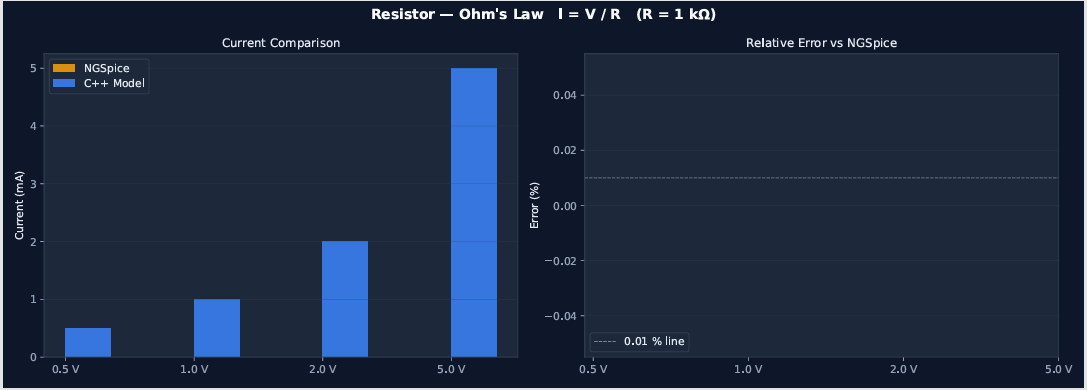
\includegraphics[width=\linewidth]{Figures/Ch5/Res-1.png}
        \caption{Resistor Simulation Verification against NGSpice (Test 1).}
        \label{fig:res_test_1}
    \end{minipage}\hfill
    \begin{minipage}{0.48\textwidth}
        \centering
        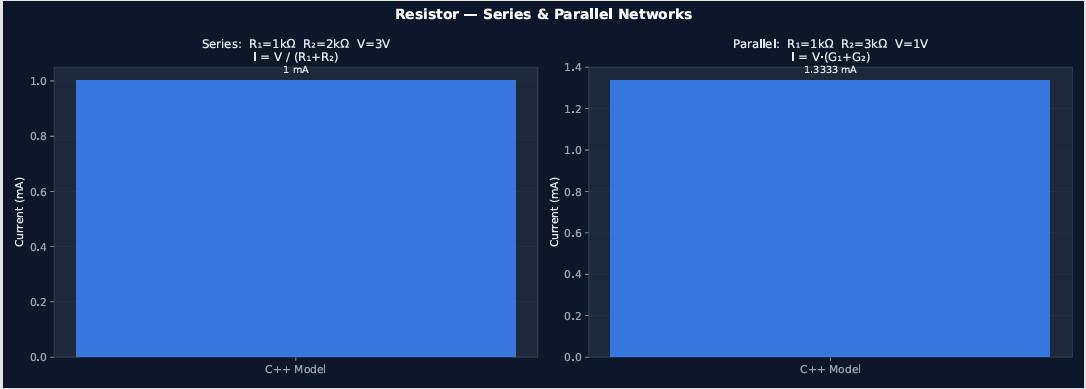
\includegraphics[width=\linewidth]{Figures/Ch5/Res-2.png}
        \caption{Resistor Simulation Verification against NGSpice (Test 2).}
        \label{fig:res_test_2}
    \end{minipage}
\end{figure}

\begin{figure}[H]
    \centering
    \begin{minipage}{0.48\textwidth}
        \centering
        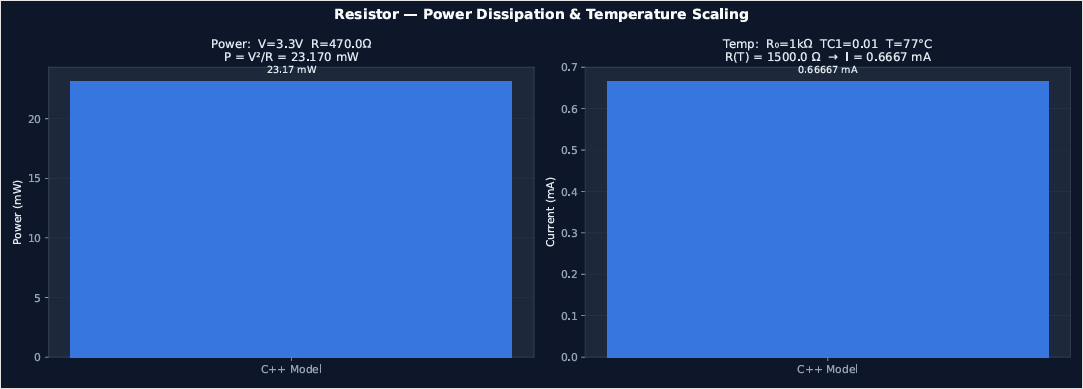
\includegraphics[width=\linewidth]{Figures/Ch5/Res-3.png}
        \caption{Resistor Simulation Verification against NGSpice (Test 3).}
        \label{fig:res_test_3}
    \end{minipage}\hfill
    \begin{minipage}{0.48\textwidth}
        \centering
        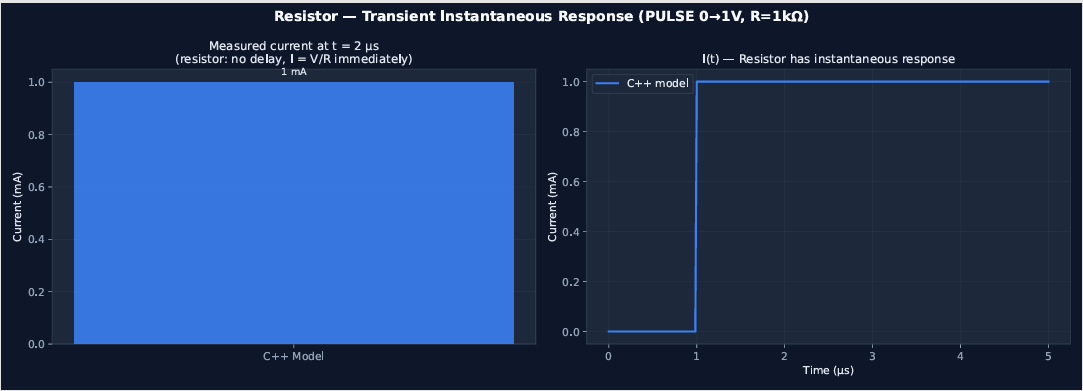
\includegraphics[width=\linewidth]{Figures/Ch5/Res-4.png}
        \caption{Resistor Simulation Verification against NGSpice (Test 4).}
        \label{fig:res_test_4}
    \end{minipage}
\end{figure}

\subsection{Capacitor}
The capacitor unit tests confirm the accuracy of state history updates, transient integration schemes, and varactor charge equations.

\subsubsection{Internal C++ Unit Tests (Google Test)}
The comprehensive Google Test suite strictly validates capacitor dynamics, transient physics, and model variants:
\begin{itemize}
    \item \textbf{DC Behaviour:} Verifies that Equivalent Series Resistance (ESR) and minimum leakage conductance (\texttt{gmin}) are correctly stamped into the conductance matrix $G$.
    \item \textbf{Transient Behaviour:} Validates Backward-Euler state integration equations, confirming step voltage currents ($i(t) = C \cdot \frac{dv}{dt}$), linear voltage ramps from constant current, RC time constants ($\tau = R C$), and current spikes from PWL slope changes.
    \item \textbf{Energy and Power:} Audits stored energy equations ($E = \frac{1}{2} C V^2$) and verifies strict power balance in RC circuits (source energy equals stored energy plus resistor dissipation).
    \item \textbf{Parameter Scaling:} Checks geometry area scaling laws and linear/quadratic temperature coefficients ($TC_1$, $TC_2$).
    \item \textbf{Model Variants:} Validates analytic integral charge equations and variable differential capacitance ($\frac{dQ}{dV}$) for non-linear varactor junctions, polynomial coefficients, and ideal linear formulations.
\end{itemize}

\subsubsection{NGSpice Verification}
Transient and varactor sweeps are compared. Figures~\ref{fig:cap_test_1} to \ref{fig:cap_test_3} demonstrate perfect agreement with NGSpice outputs.

\begin{figure}[H]
    \centering
    \begin{minipage}{0.48\textwidth}
        \centering
        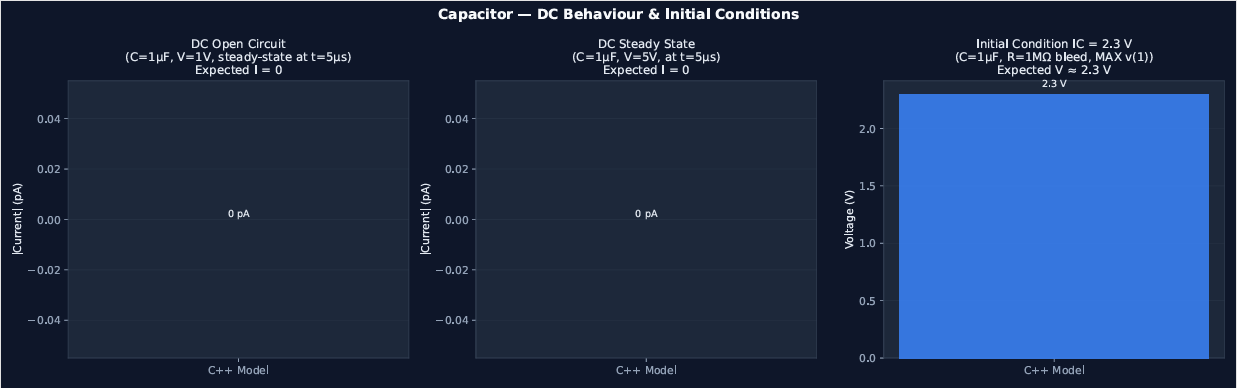
\includegraphics[width=\linewidth]{Figures/Ch5/Cap-1.png}
        \caption{Capacitor Voltage Verification (Test 1).}
        \label{fig:cap_test_1}
    \end{minipage}\hfill
    \begin{minipage}{0.48\textwidth}
        \centering
        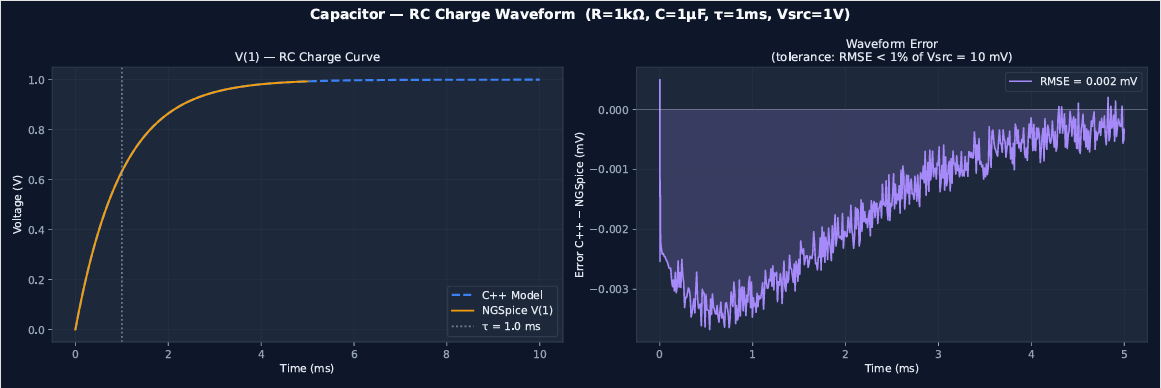
\includegraphics[width=\linewidth]{Figures/Ch5/Cap-2.png}
        \caption{Capacitor Current Verification (Test 2).}
        \label{fig:cap_test_2}
    \end{minipage}
\end{figure}

\begin{figure}[H]
    \centering
    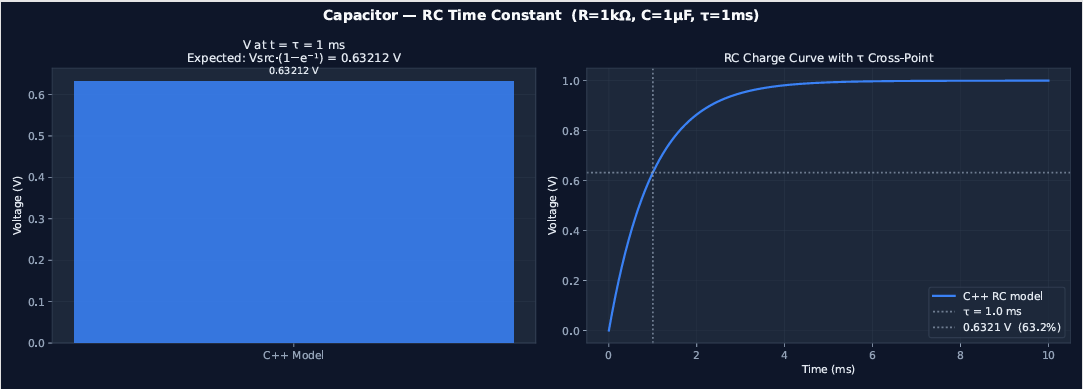
\includegraphics[width=0.6\textwidth]{Figures/Ch5/Cap-3.png}
    \caption{Capacitor Charge vs. Voltage Characteristic under Varactor Mode (Test 3).}
    \label{fig:cap_test_3}
\end{figure}

\subsection{Inductor}
Inductor unit tests validate MNA branch current formulations, energy conservation, and parameter scaling laws.

\subsubsection{Internal C++ Unit Tests (Google Test)}
Google Test validation sweeps frequency and time to confirm the impedance equations and verifies energy conservation ($\Delta E = \int P dt$) in dynamic RL networks:
\begin{itemize}
    \item \textbf{DC Operating Point:} Validates that the inductor behaves as a short circuit with series resistance $R_s$, showing correct branch current topology matrix entries.
    \item \textbf{AC Frequency Sweeps:} Confirms the frequency-dependent impedance relationship $Z(j\omega) = R_s + j\omega L$, stamping $L$ in the dynamic $C$ matrix branch diagonal.
    \item \textbf{Transient Integration:} Verifies the Backward Euler integration current updates across transient steps.
    \item \textbf{Energy Auditing:} Audits the power balance ($\Delta E = \int P dt$), confirming energy conservation within numerical tolerances.
    \item \textbf{Parameter Scaling:} Verifies that area and temperature dependencies scale the nominal inductance correctly using $TC_1$ and $TC_2$ coefficients.
\end{itemize}

\subsubsection{NGSpice Verification}
Figures~\ref{fig:ind_test_1} to \ref{fig:ind_test_4} show the comparison of impedance magnitude, transient step, energy tracking, and area/temperature scaling against NGSpice.

\begin{figure}[H]
    \centering
    \begin{minipage}{0.48\textwidth}
        \centering
        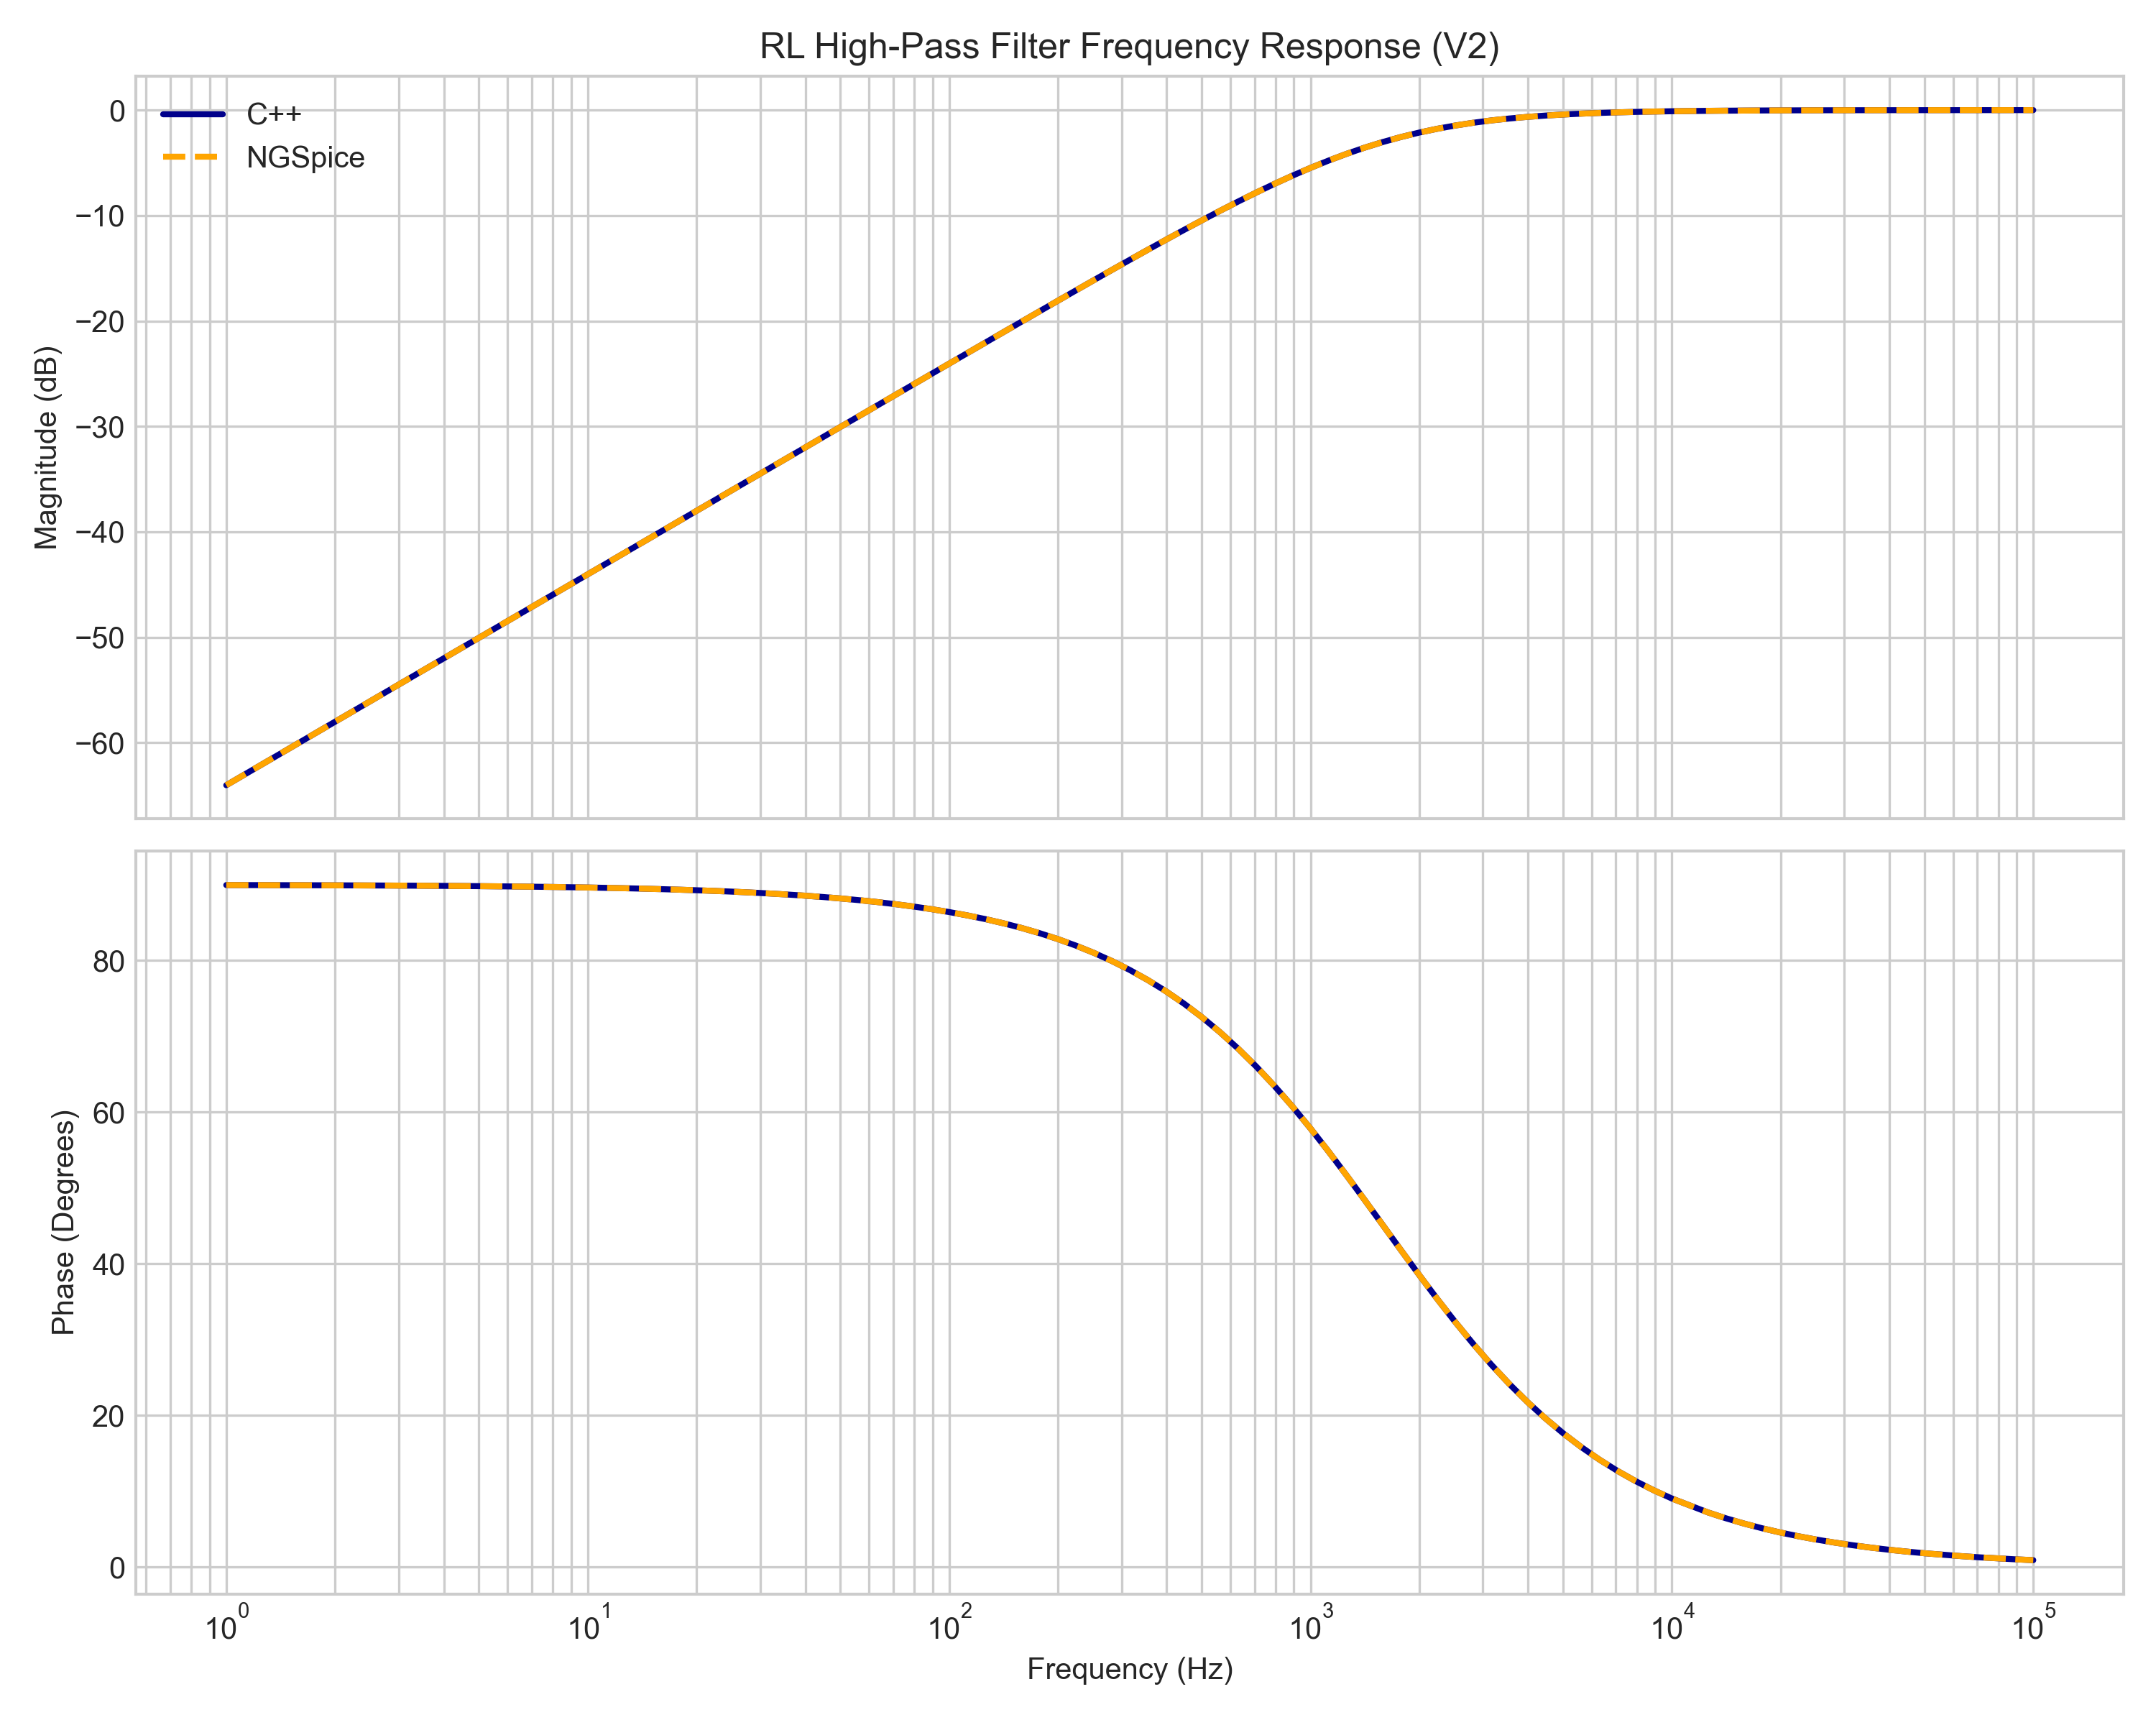
\includegraphics[width=\linewidth]{Figures/Ch5/Inductor-1.png}
        \caption{Inductor AC Impedance Validation.}
        \label{fig:ind_test_1}
    \end{minipage}\hfill
    \begin{minipage}{0.48\textwidth}
        \centering
        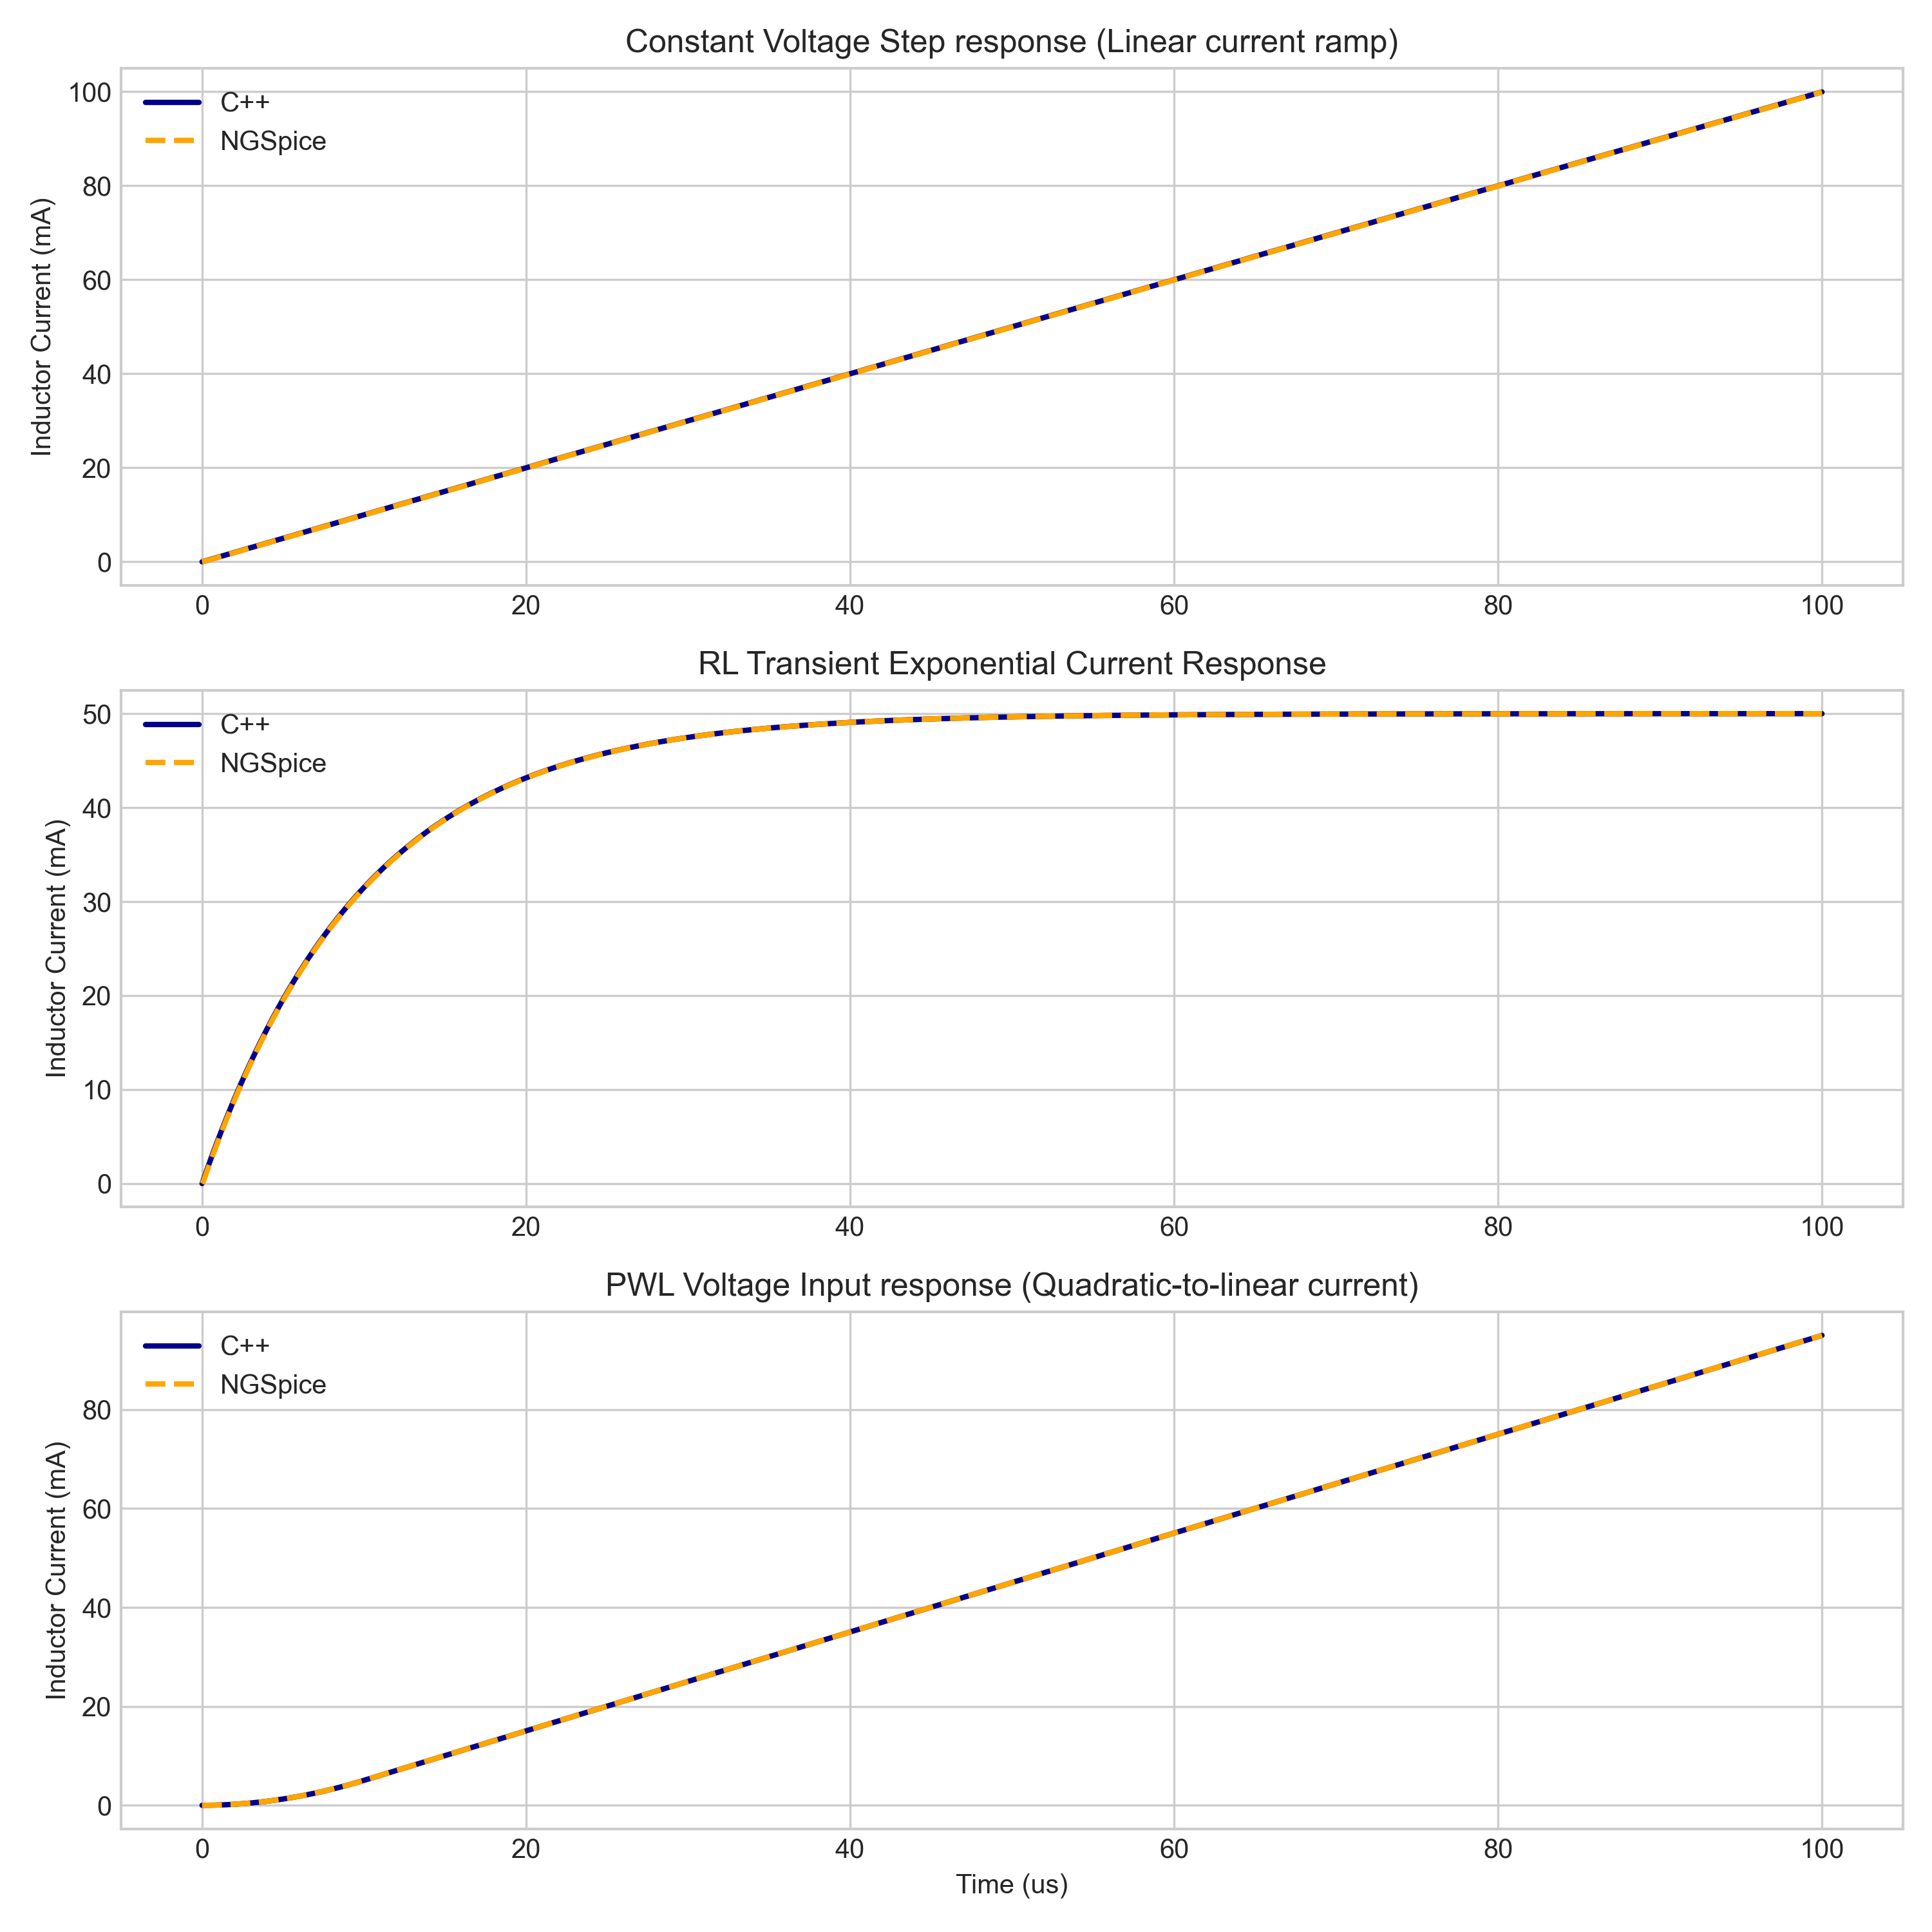
\includegraphics[width=\linewidth]{Figures/Ch5/Inductor-2.png}
        \caption{Inductor Transient Step Response.}
        \label{fig:ind_test_2}
    \end{minipage}
\end{figure}

\begin{figure}[H]
    \centering
    \begin{minipage}{0.48\textwidth}
        \centering
        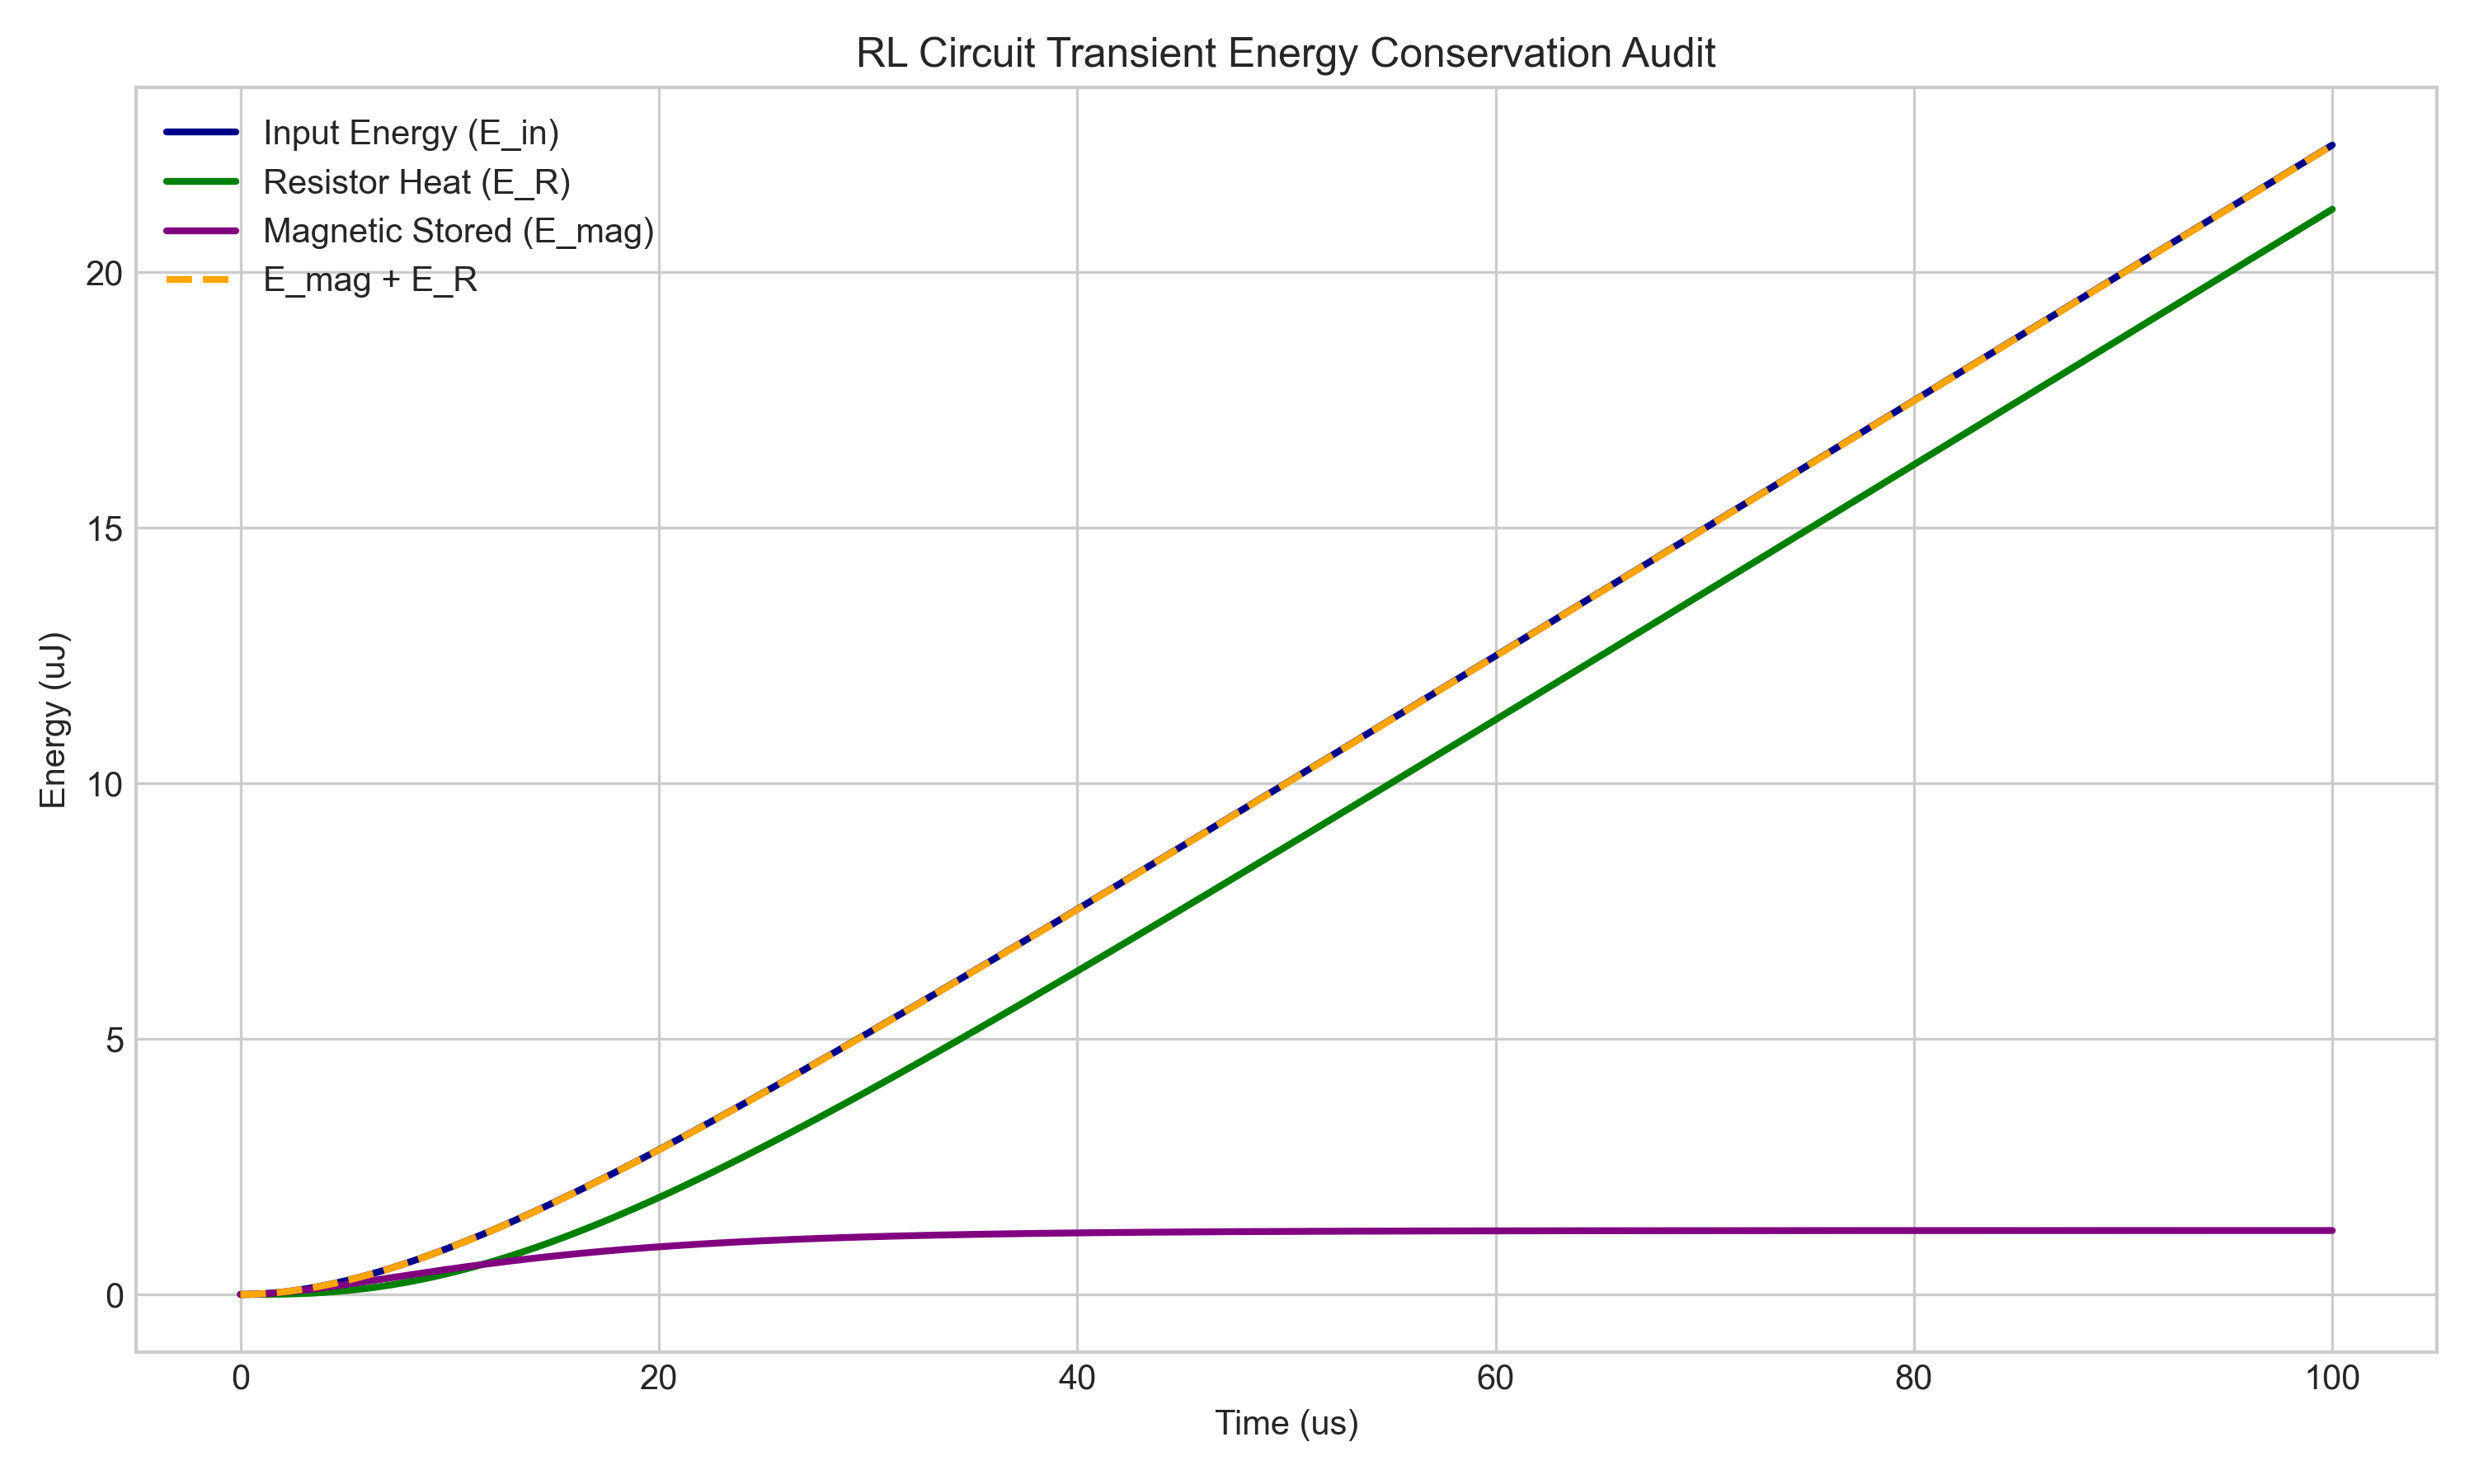
\includegraphics[width=\linewidth]{Figures/Ch5/Inductor-3.png}
        \caption{Inductor Energy Conservation Balance.}
        \label{fig:ind_test_3}
    \end{minipage}\hfill
    \begin{minipage}{0.48\textwidth}
        \centering
        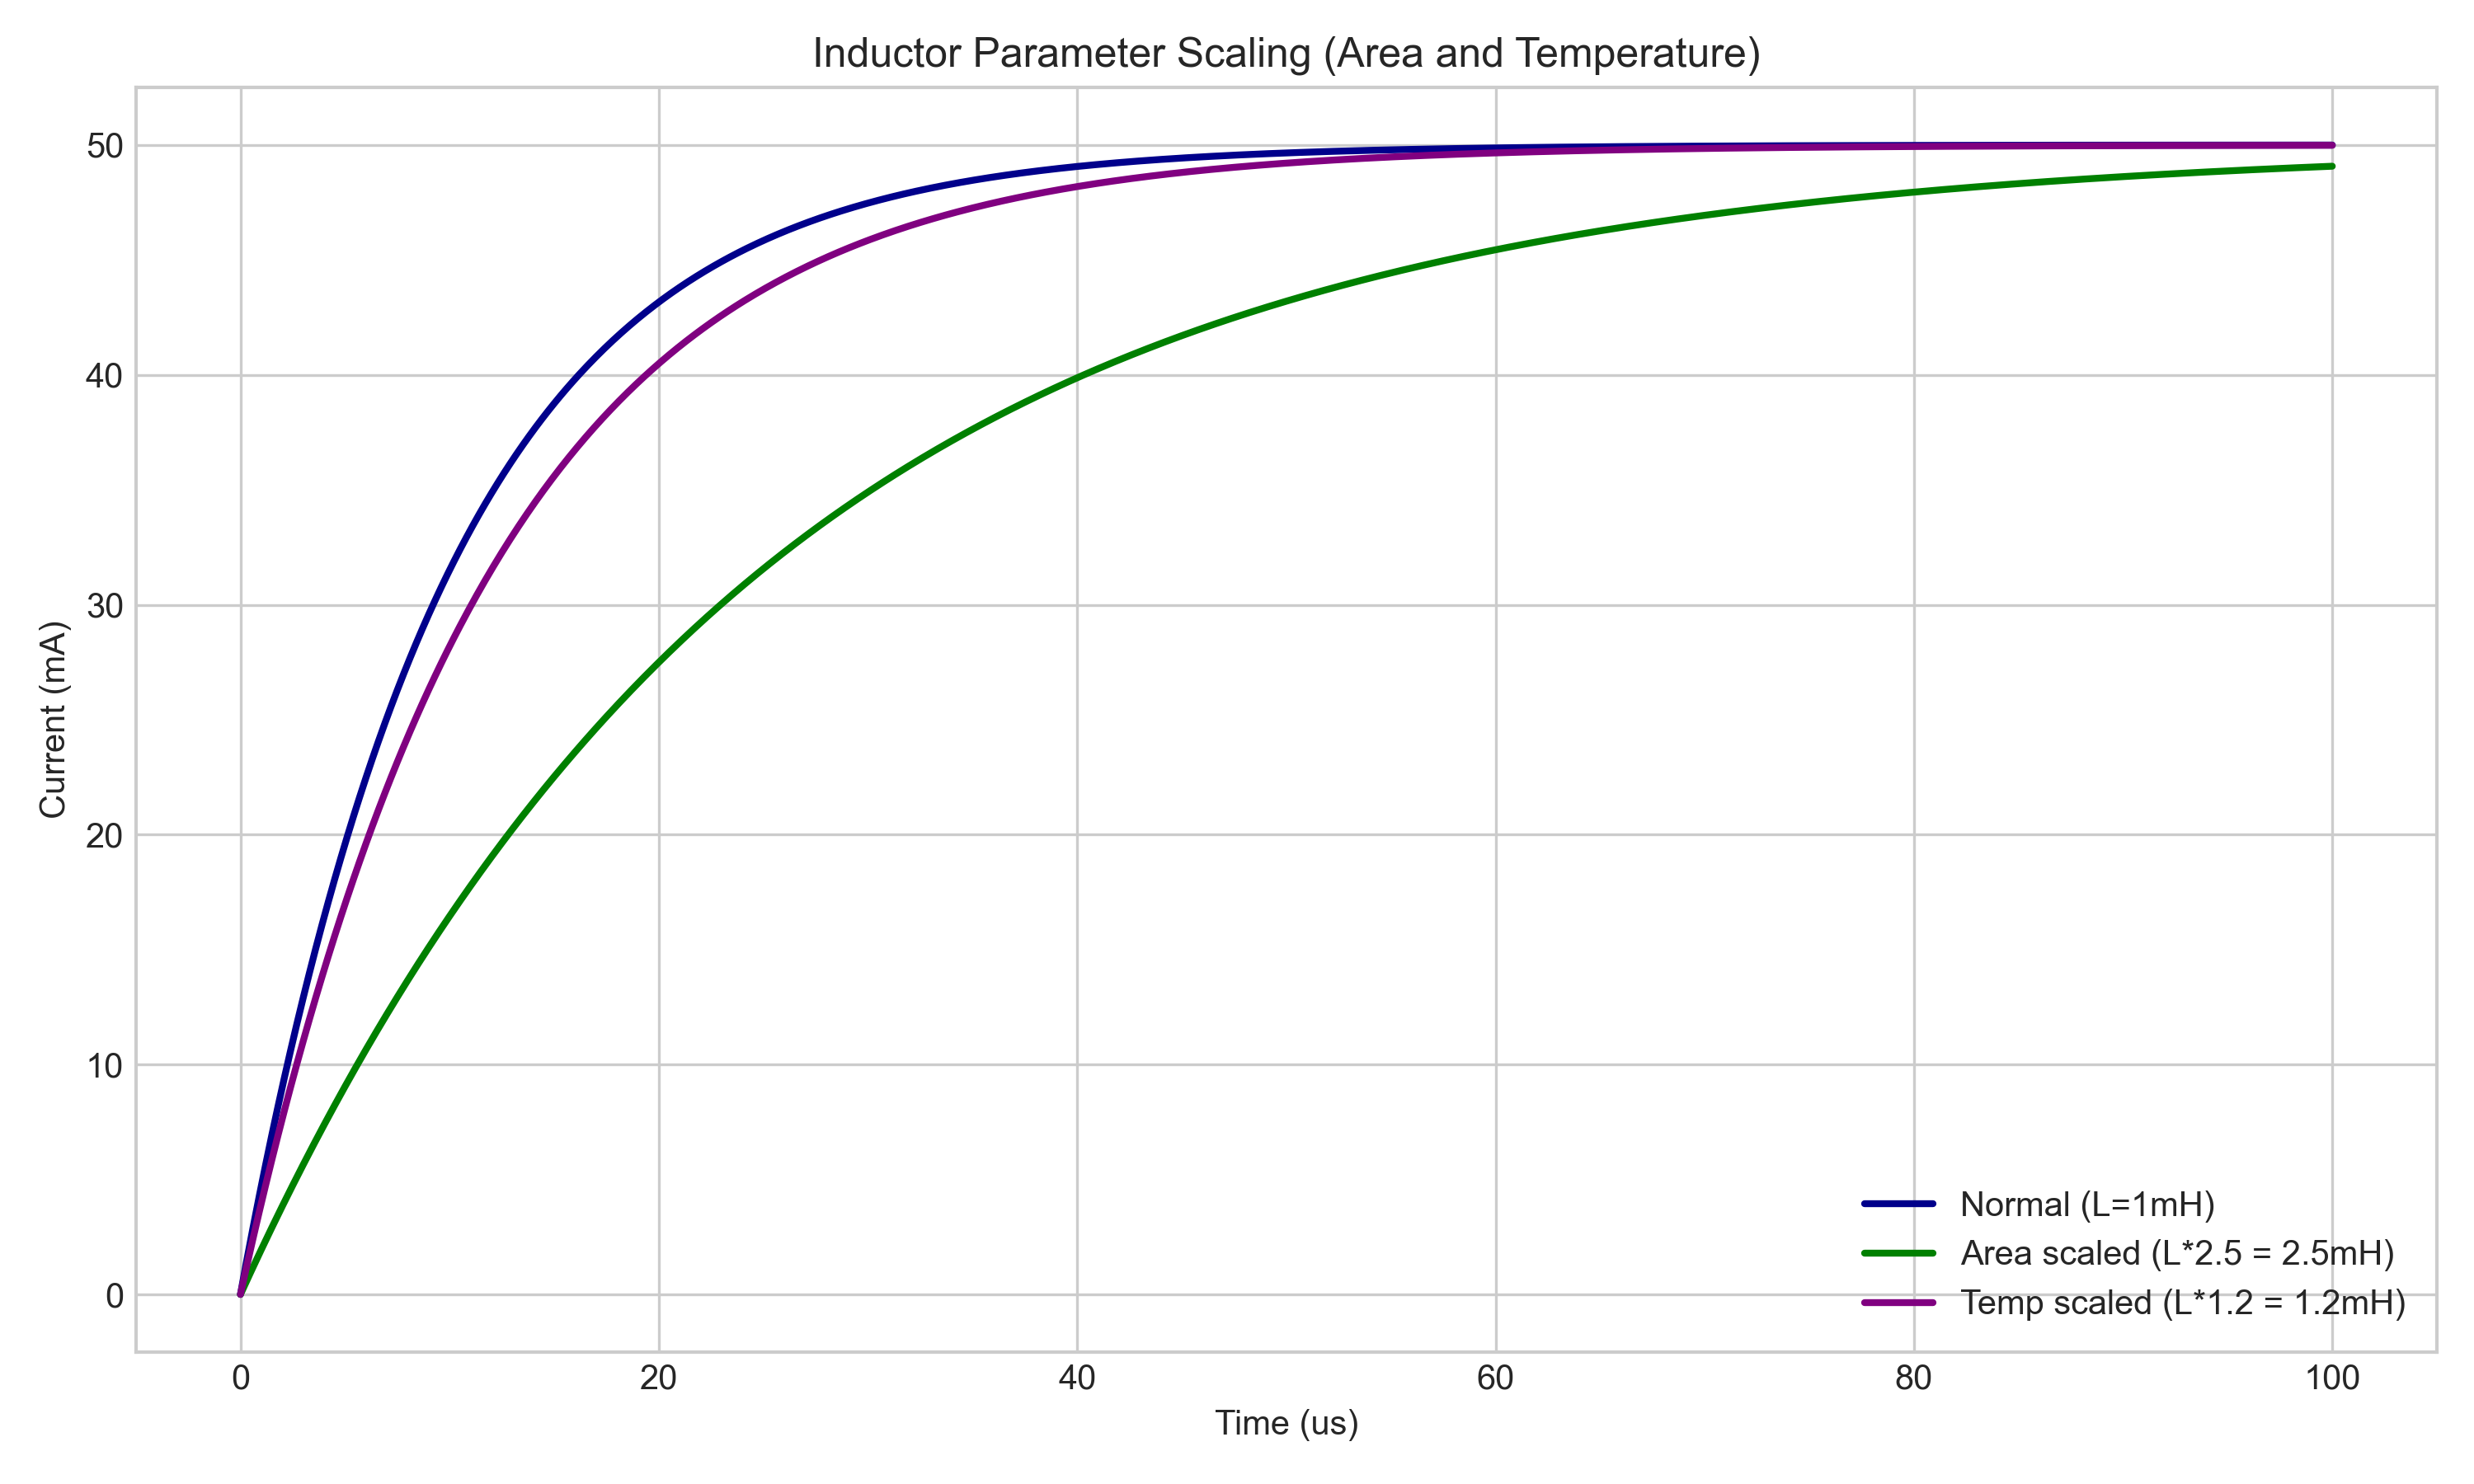
\includegraphics[width=\linewidth]{Figures/Ch5/Inductor-4.png}
        \caption{Inductor Area and Temp Scaling.}
        \label{fig:ind_test_4}
    \end{minipage}
\end{figure}

\subsection{Diode}
Diode unit tests focus on non-linear Shockley characteristics, convergence, and voltage limiting.

\subsubsection{Internal C++ Unit Tests (Google Test)}
Test cases sweep bias conditions to evaluate the Shockley forward current, verify reverse breakdown transitions, and stress-test the `pnjlim` convergence algorithm under near-singular updates:
\begin{itemize}
    \item \textbf{Forward I-V Sweep:} Validates Shockley forward current equations across temperature and voltage sweeps.
    \item \textbf{Reverse Breakdown:} Verifies the reverse breakdown voltage ($B_V$) and breakdown current ($I_{BV}$) transitions.
    \item \textbf{Gmin Leakage:} Confirms that the minimum parallel leakage conductance ($g_{\text{min}}$) is correctly stamped under large reverse bias conditions.
    \item \textbf{Junction and Diffusion Capacitance:} Validates the transit time ($\tau_D$) diffusion capacitance and voltage-dependent depletion capacitance transitions.
    \item \textbf{Convergence and Limiting:} Proves that the `pnjlim` algorithm prevents exponential overflow and guarantees rapid Newton-Raphson convergence.
\end{itemize}

\subsubsection{NGSpice Verification}
Figures~\ref{fig:diode_test_1} to \ref{fig:diode_test_4} depict the diode's forward I-V characteristics, reverse breakdown current, reverse Gmin leakage, and junction capacitance.

\begin{figure}[H]
    \centering
    \begin{minipage}{0.48\textwidth}
        \centering
        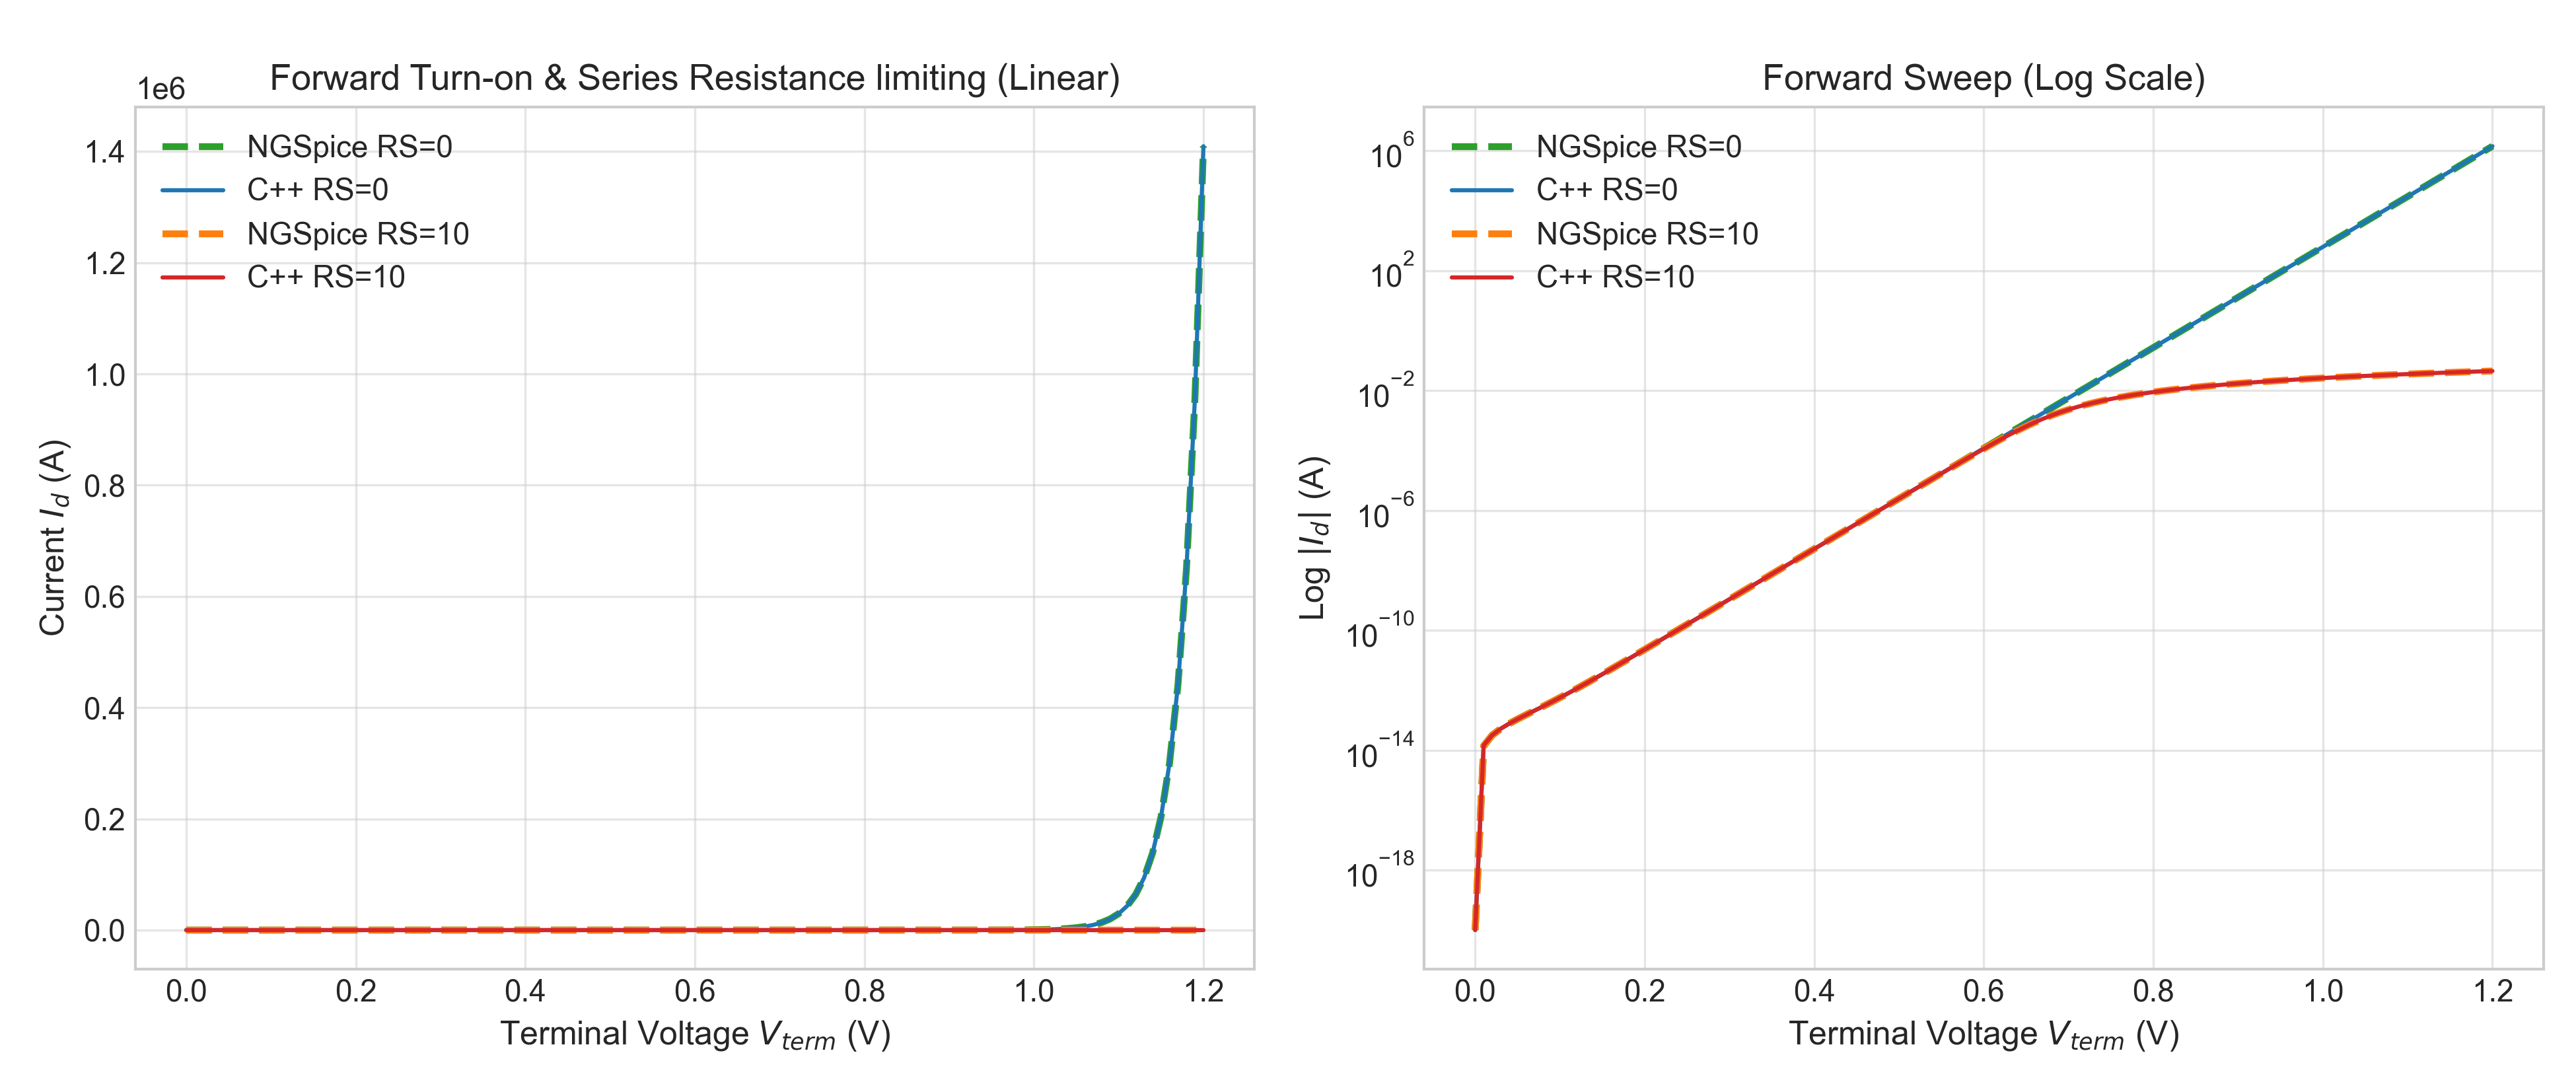
\includegraphics[width=\linewidth]{Figures/Ch5/Diode-1.png}
        \caption{Diode Forward I-V Characteristic.}
        \label{fig:diode_test_1}
    \end{minipage}\hfill
    \begin{minipage}{0.48\textwidth}
        \centering
        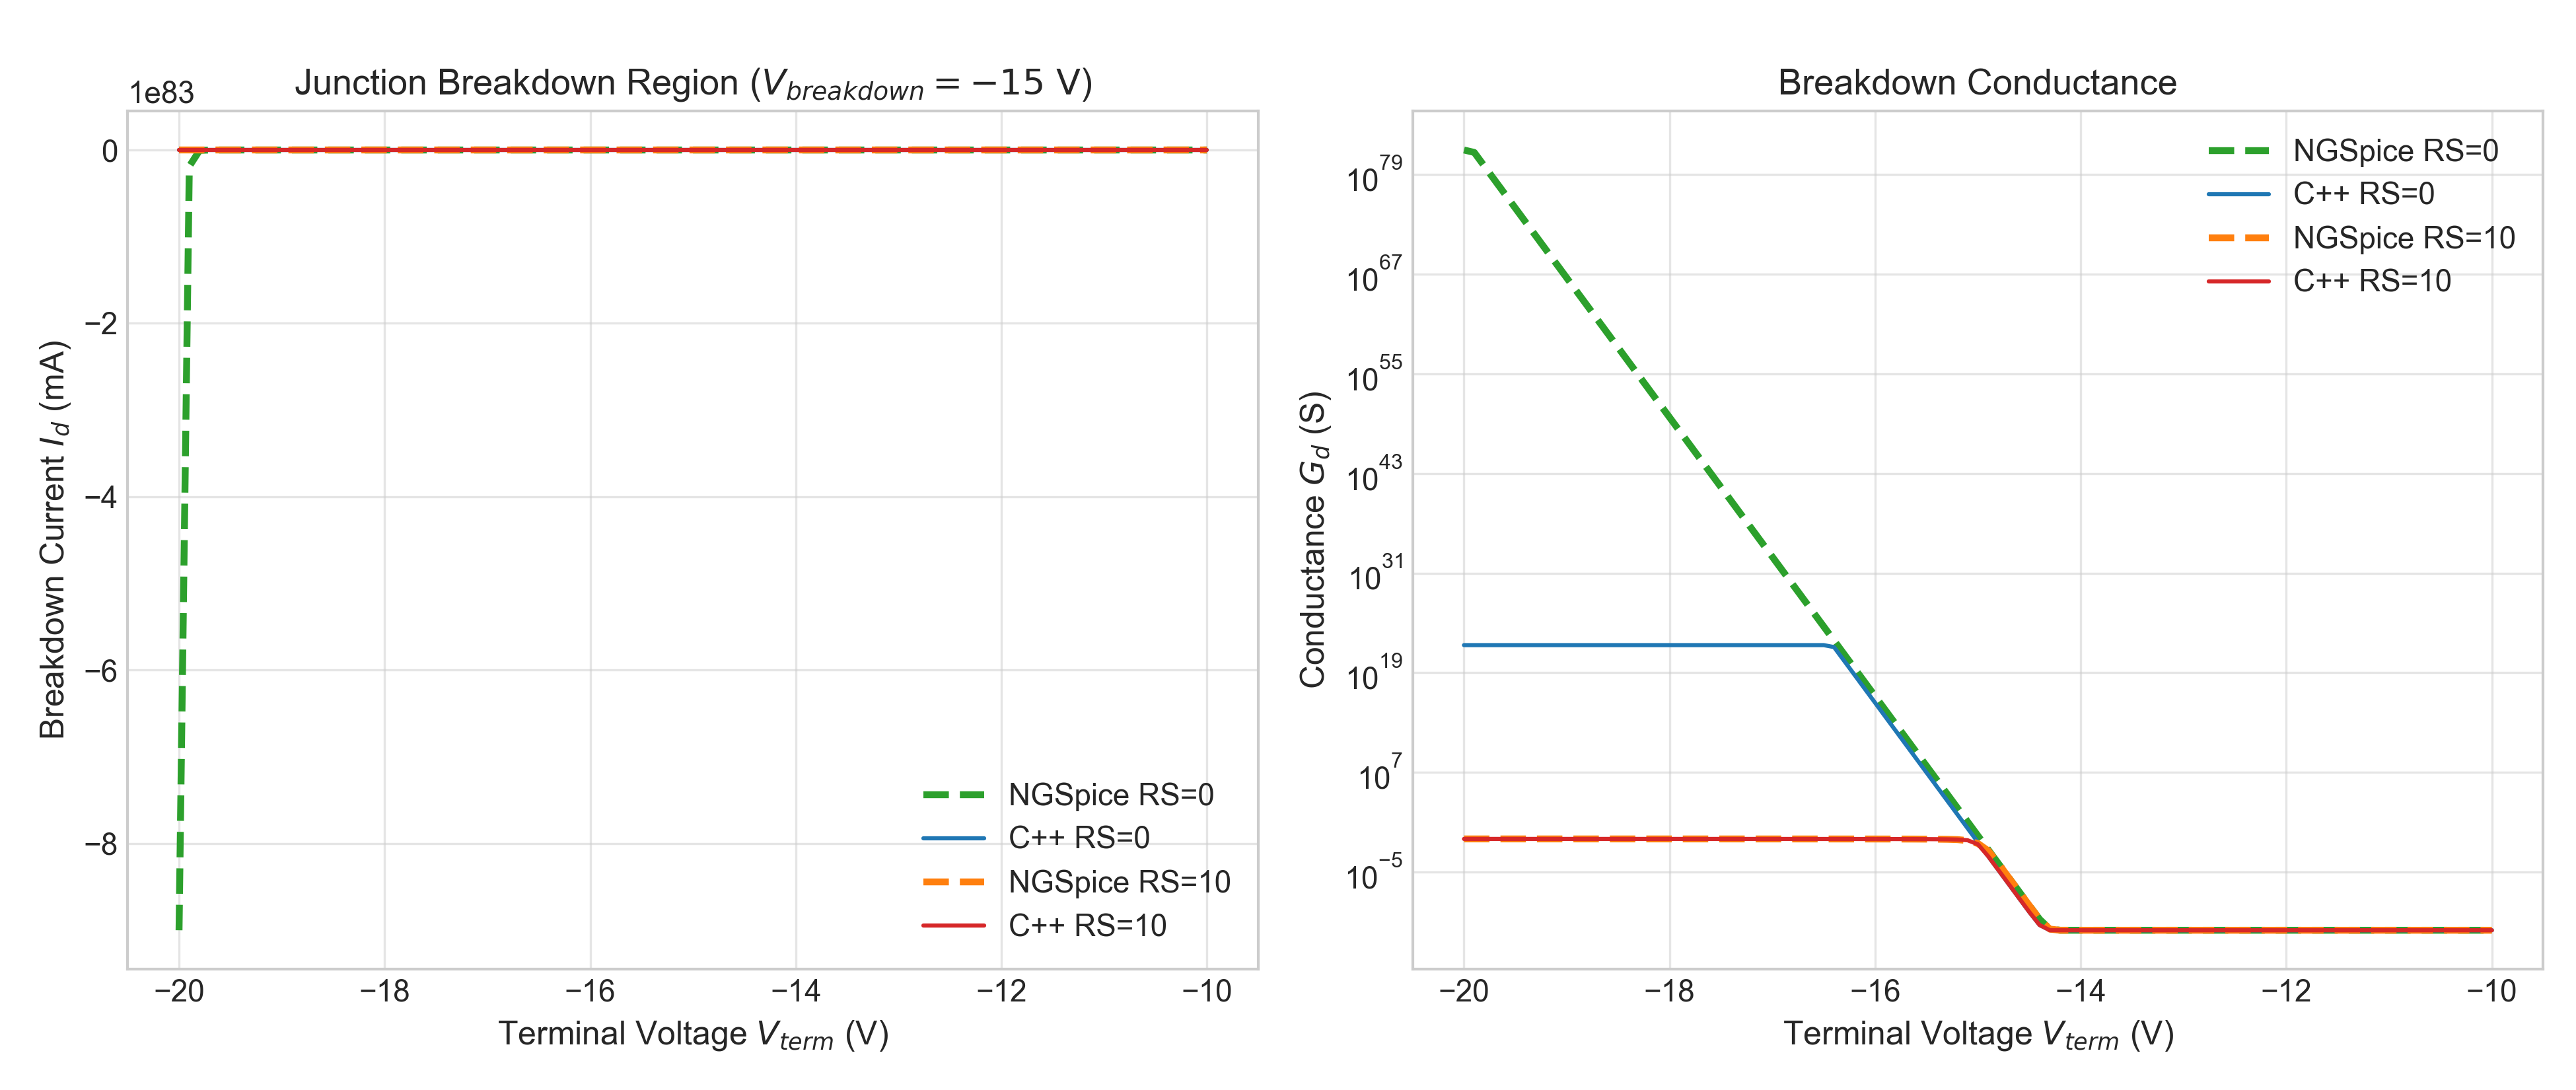
\includegraphics[width=\linewidth]{Figures/Ch5/Diode-2.png}
        \caption{Diode Reverse Breakdown Sweep.}
        \label{fig:diode_test_2}
    \end{minipage}
\end{figure}

\begin{figure}[H]
    \centering
    \begin{minipage}{0.48\textwidth}
        \centering
        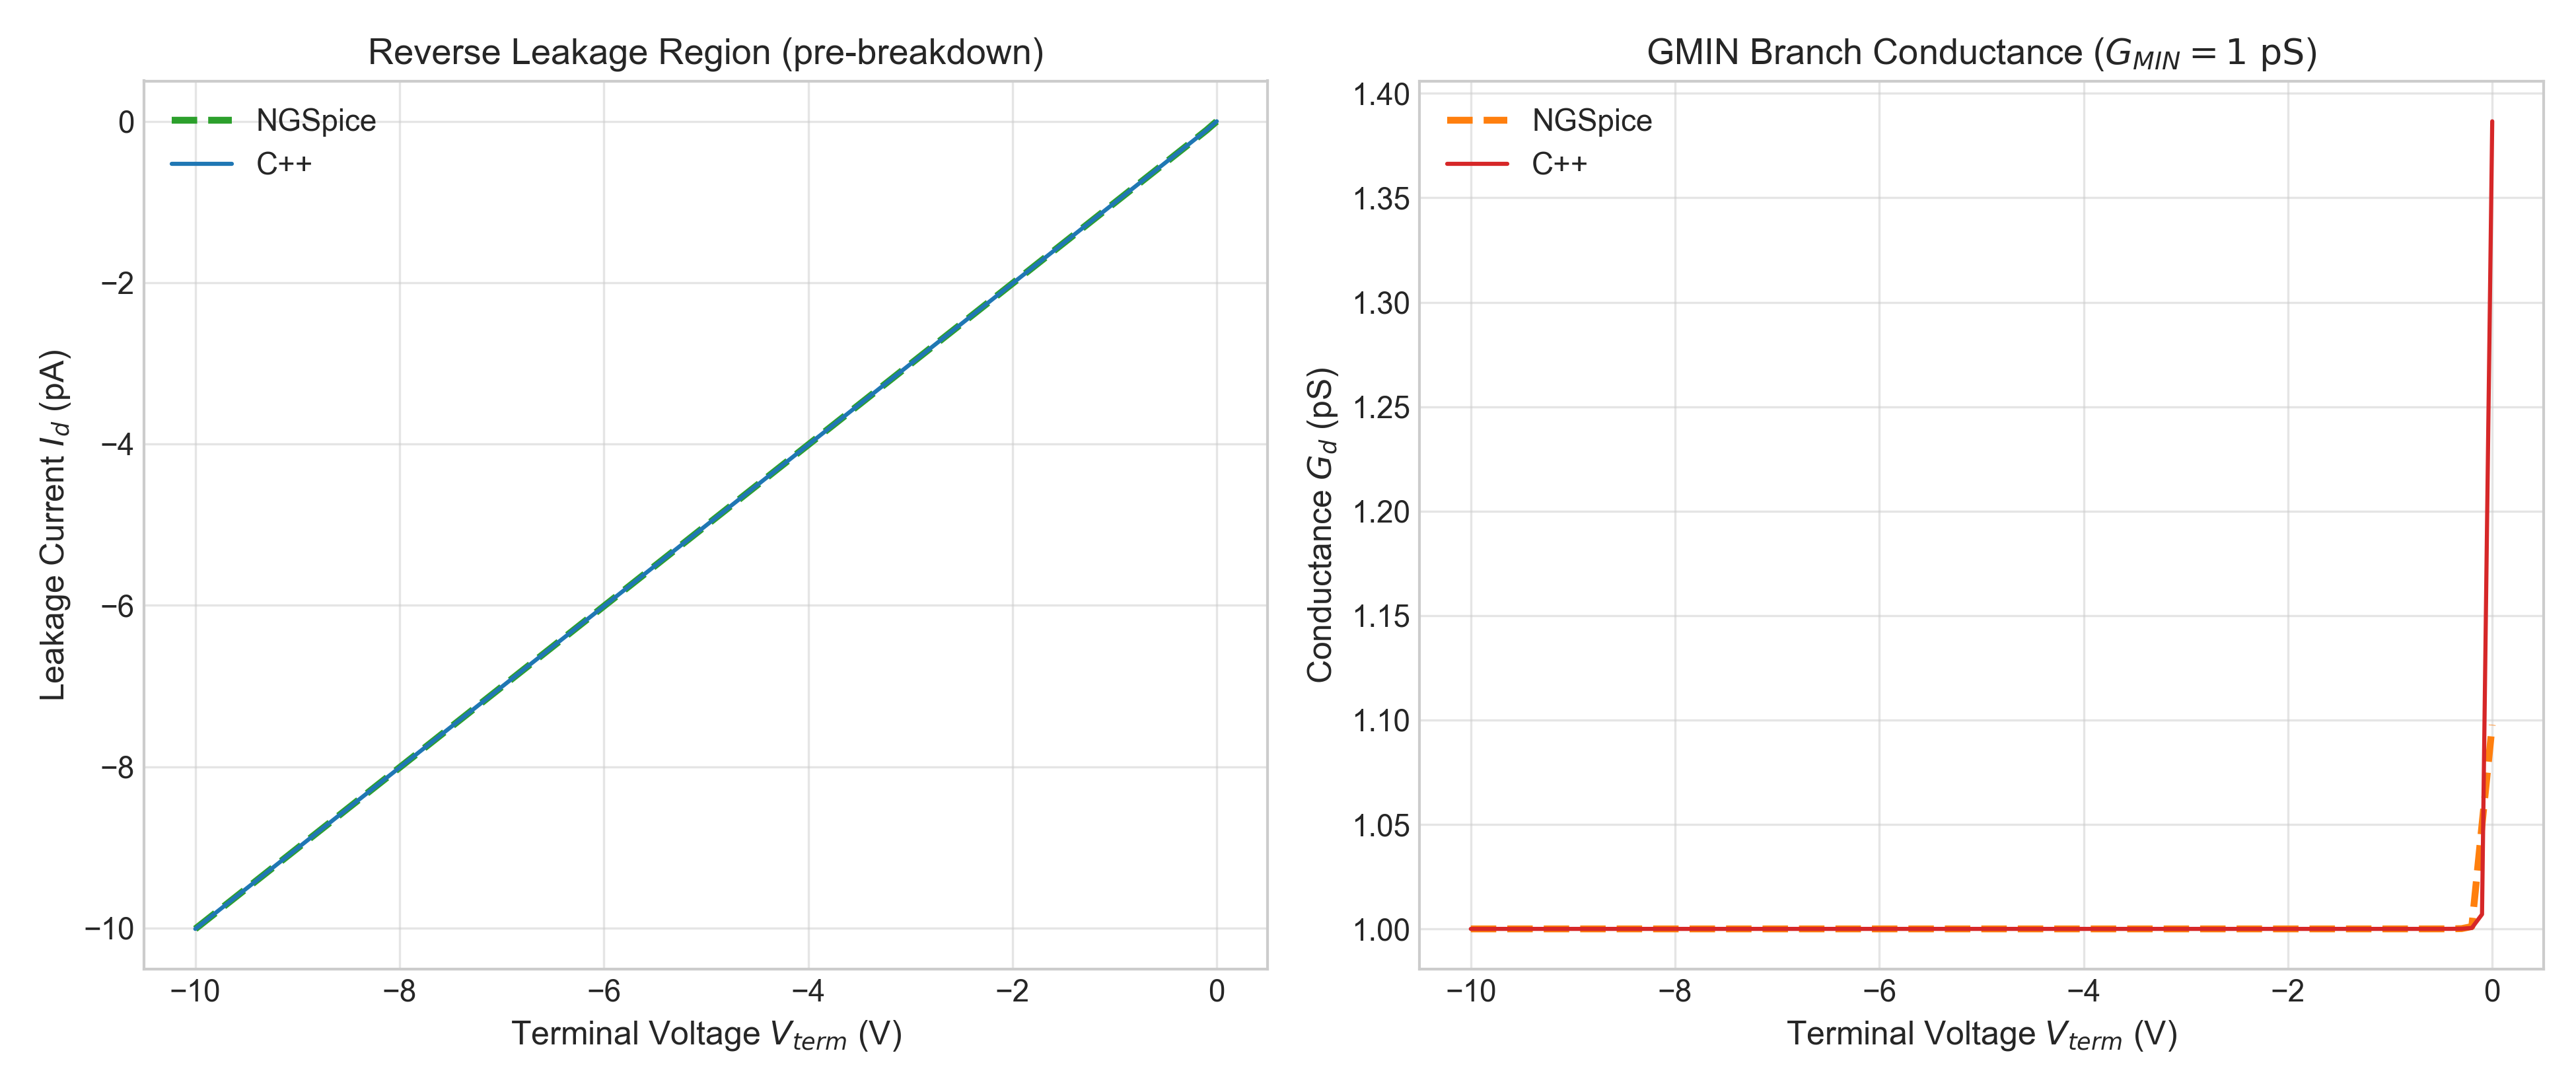
\includegraphics[width=\linewidth]{Figures/Ch5/Diode-3.png}
        \caption{Diode Reverse Gmin Current Leakage.}
        \label{fig:diode_test_3}
    \end{minipage}\hfill
    \begin{minipage}{0.48\textwidth}
        \centering
        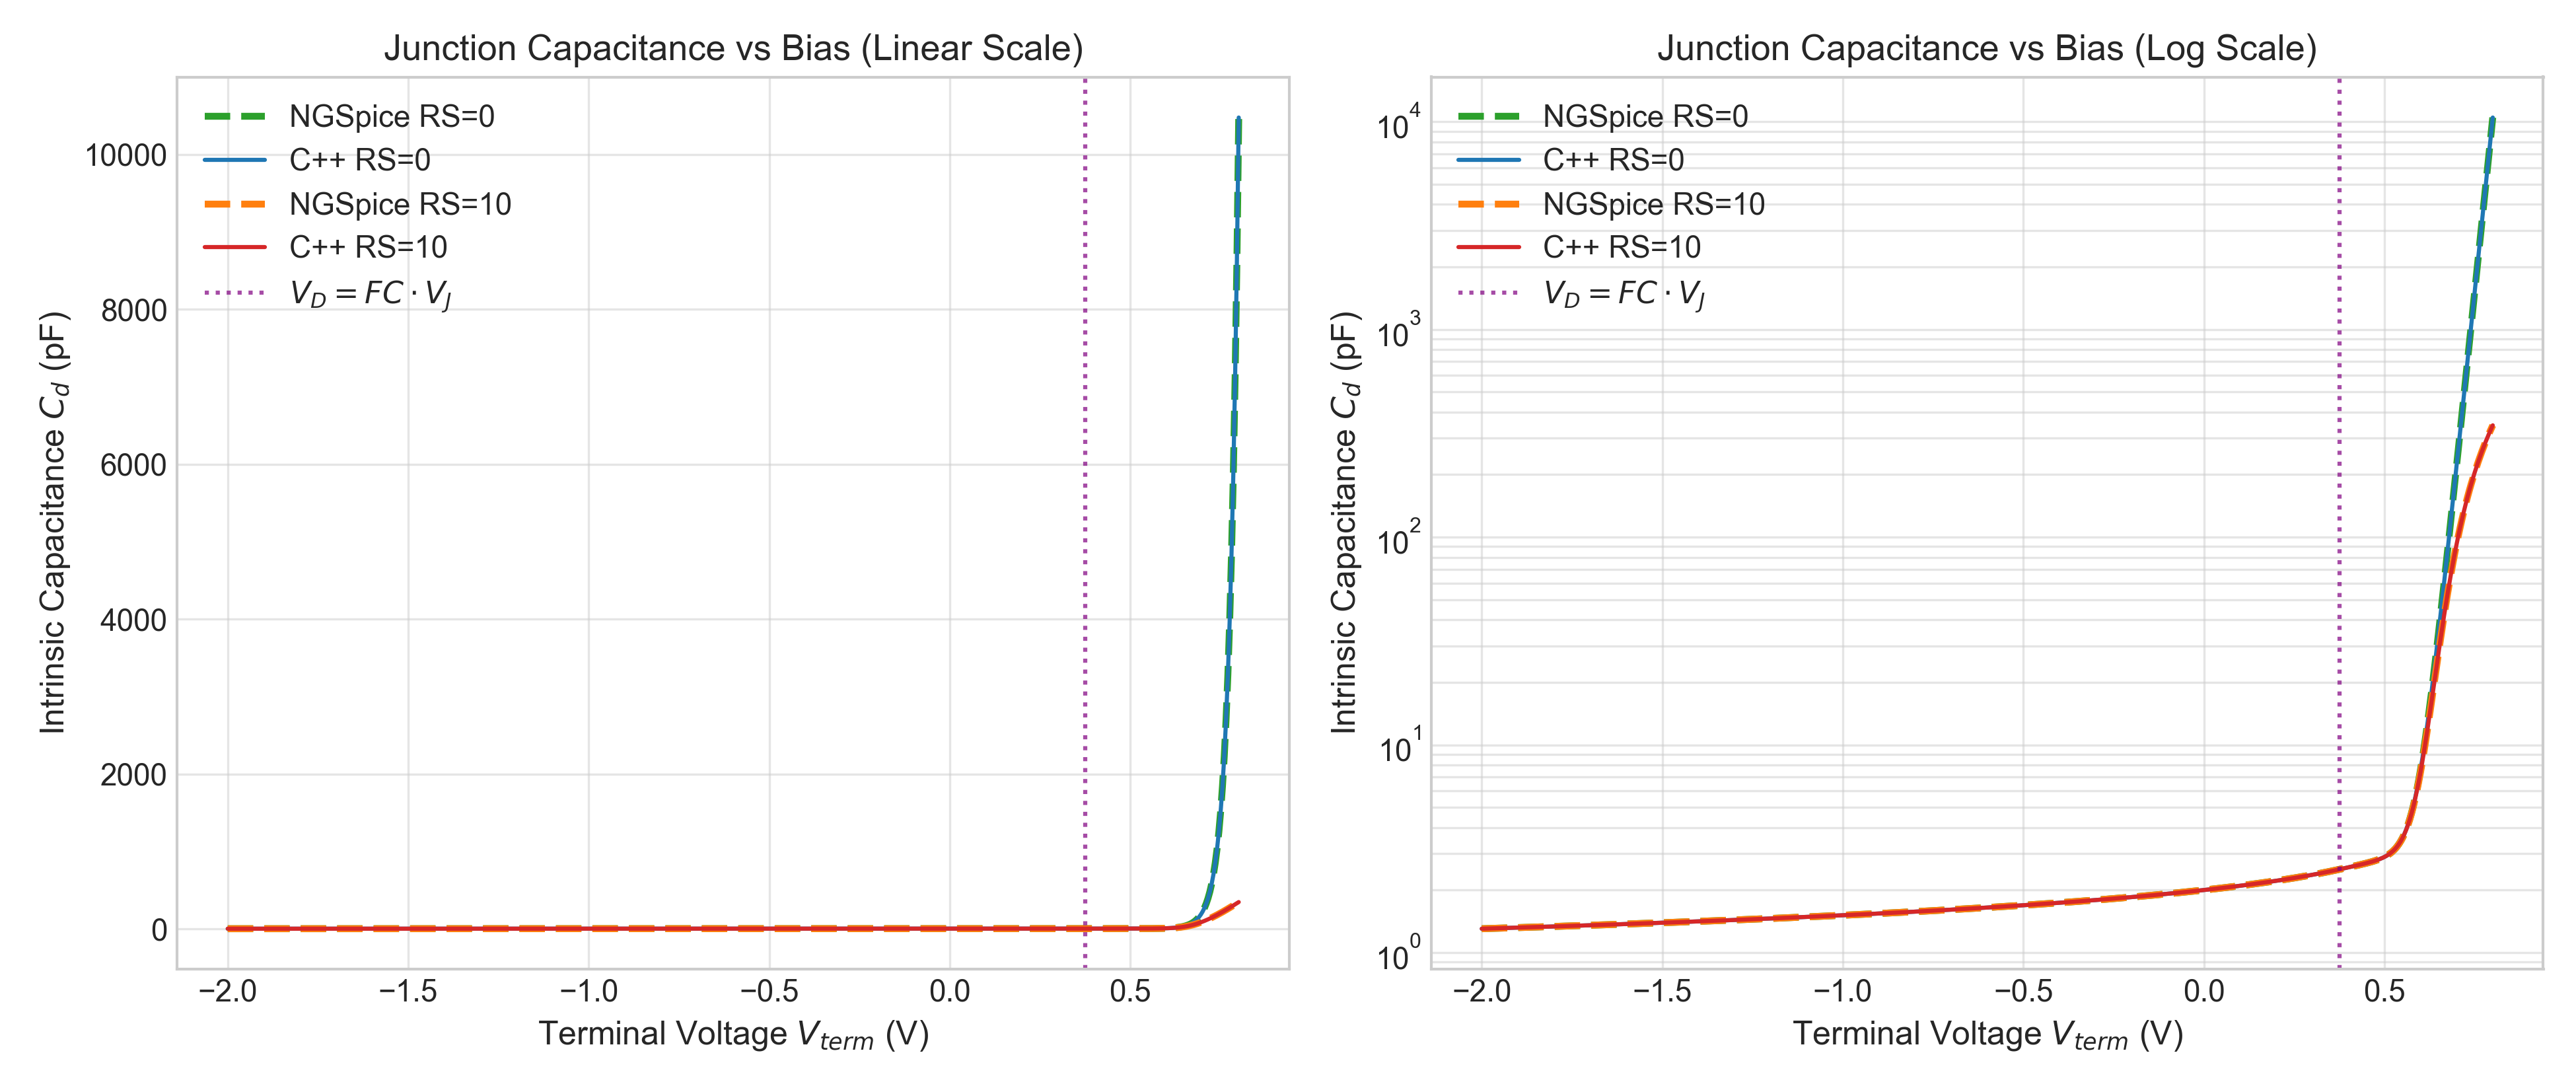
\includegraphics[width=\linewidth]{Figures/Ch5/Diode-4.png}
        \caption{Diode Junction Capacitance vs. Bias.}
        \label{fig:diode_test_4}
    \end{minipage}
\end{figure}

\subsection{Junction Field-Effect Transistor (JFET)}
JFET tests focus on active-channel square-law equations and small-signal conductances.

\subsubsection{Internal C++ Unit Tests (Google Test)}
The Google Test suite for the JFET thoroughly validates its static, dynamic, and thermal behaviors:
\begin{itemize}
    \item \textbf{DC Behavior (Static I-V):} Validates that the device enters cutoff when $|V_{gs}| \ge |V_p|$, verifies Ohmic and Saturation region boundaries, and confirms Channel-Length Modulation (CLM) effects on the output slope.
    \item \textbf{Small-Signal Derivatives:} Validates the analytic formulas for transconductance ($g_m$) and output conductance ($g_{ds}$) across regions, and ensures strict current continuity at the Ohmic-Saturation boundary.
    \item \textbf{Gate Junction Behavior:} Verifies the reverse gate leakage current ($I_S$) and checks the exponential voltage dependence under forward bias.
    \item \textbf{AC and Capacitances:} Ensures correct bias-dependent calculations of $C_{gs}$ and $C_{gd}$ under reverse and forward biases, and verifies the MNA C-matrix AC stamps.
    \item \textbf{Transient and MNA Stamping:} Verifies that \texttt{updateState()} correctly computes all operating point quantities and that the DC G-matrix correctly stamps the conductances.
    \item \textbf{Temperature Scaling:} Confirms that $I_{DSS}$ scales with $T^{-1.5}$, $V_p$ shifts linearly by $2.5\text{ mV}/^\circ\text{C}$, and the gate saturation current $I_S$ scales with $T^3$.
\end{itemize}

\subsubsection{NGSpice Verification}
Figures~\ref{fig:jfet_test_1} to \ref{fig:jfet_test_3} show the JFET output characteristics, transfer characteristics, and gate capacitances.

\begin{figure}[H]
    \centering
    \begin{minipage}{0.48\textwidth}
        \centering
        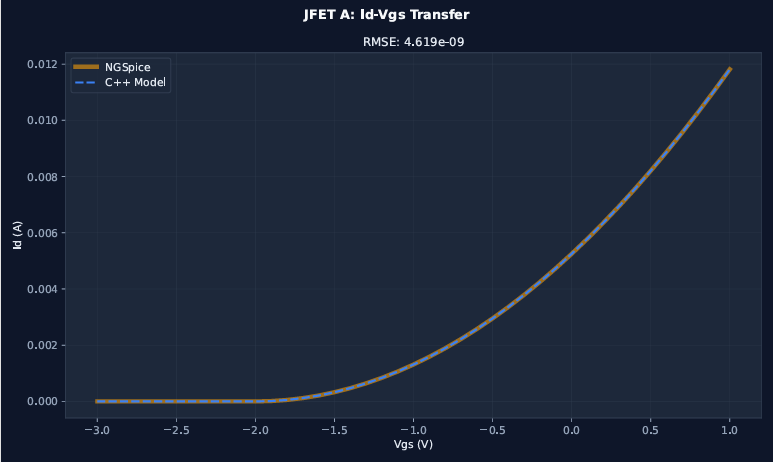
\includegraphics[width=\linewidth]{Figures/Ch5/JFET-1.png}
        \caption{JFET Transfer Characteristics ($I_d$ vs. $V_{gs}$).}
        \label{fig:jfet_test_1}
    \end{minipage}\hfill
    \begin{minipage}{0.48\textwidth}
        \centering
        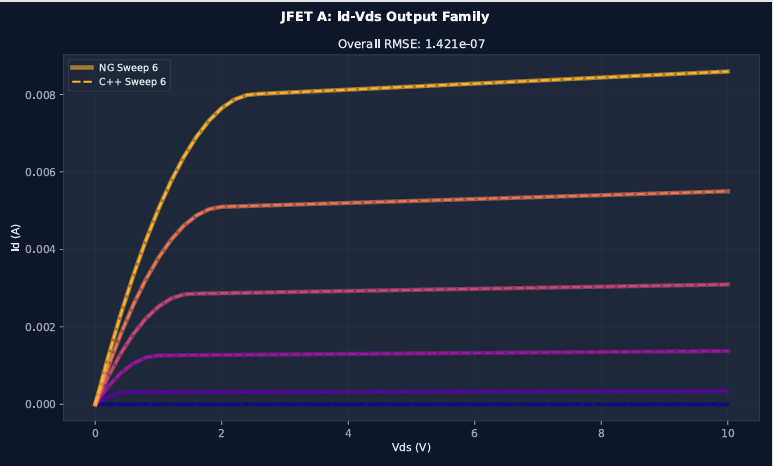
\includegraphics[width=\linewidth]{Figures/Ch5/JFET-2.png}
        \caption{JFET Output Characteristics ($I_d$ vs. $V_{ds}$).}
        \label{fig:jfet_test_2}
    \end{minipage}
\end{figure}

\begin{figure}[H]
    \centering
    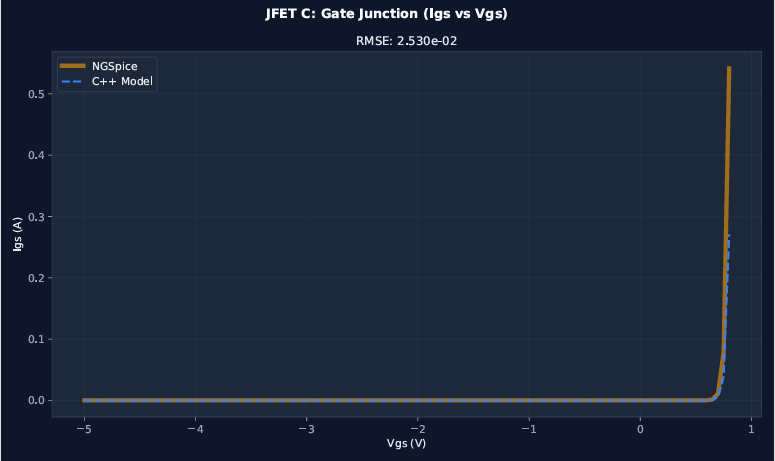
\includegraphics[width=0.6\textwidth]{Figures/Ch5/JFET-3.png}
    \caption{JFET Gate-Source and Gate-Drain Junction Capacitance.}
    \label{fig:jfet_test_3}
\end{figure}

\subsection{Metal-Oxide-Semiconductor Field-Effect Transistor (MOSFET)}
MOSFET unit tests validate multi-level models, symmetric finite differences for conductances, and short-channel effects.

\subsubsection{Internal C++ Unit Tests (Google Test)}
The MOSFET Google Test suite spans over 800 lines of rigorous validation across its physics and implementation models (Levels 1, 2, 3, and BSIM4). It verifies 10 distinct categories:
\begin{itemize}
    \item \textbf{Basic DC Behaviour:} Validates $I_d-V_{gs}$ transfers, $I_d-V_{ds}$ output curves with channel-length modulation, body effect threshold shifts, and long/short-channel properties.
    \item \textbf{Small-Signal Derivatives:} Verifies numeric/analytical accuracy and continuity across region boundaries for transconductance ($g_m$), output conductance ($g_{ds}$), and body transconductance ($g_{mb}$).
    \item \textbf{Subthreshold \& Leakage:} Validates exponential subthreshold slope and off-state leakage currents.
    \item \textbf{Body Diode \& Junctions:} Confirms voltage-dependent junction capacitances, forward bias exponential currents, and breakdown/avalanche current limits.
    \item \textbf{Capacitances \& Charge:} Ensures Ward-Dutton charge conservation ($Q_g+Q_d+Q_s+Q_b=0$) and validates Meyer-model capacitances ($C_{gs}, C_{gd}, C_{gb}$).
    \item \textbf{AC / MNA Stamping:} Verifies DC/AC matrix population and correct Norton source KCL summation signs.
    \item \textbf{Transient Behaviour:} Confirms $V_{gs}$ step responses, $Q_g$ transient charge evolution, and C-matrix stamps.
    \item \textbf{Temperature Scaling:} Confirms exact proportional scaling rules at $-40^\circ\text{C}$, $27^\circ\text{C}$, and $125^\circ\text{C}$ for threshold voltages and mobility ($KP$).
    \item \textbf{Geometry Scaling:} Verifies current proportionality with $W/L$ ratios and ensures numeric stability at extreme sub-micron geometries.
    \item \textbf{Model-Specific Parameters:} Validates Level 1 $\lambda$/$V_{TO}$ sensitivity, Level 3 DIBL ($\eta$)/mobility degradation ($\theta$), and BSIM4 deep-submicron parameter scaling.
\end{itemize}

\subsubsection{NGSpice Verification}
Figures~\ref{fig:mos_test_1} to \ref{fig:mos_test_11} display the comprehensive NGSpice verification plots for the MOSFET, validating output characteristics, transfer curves, subthreshold conduction, and various level-specific physics across the simulation engine.

\begin{figure}[H]
    \centering
    \begin{minipage}{0.48\textwidth}
        \centering
        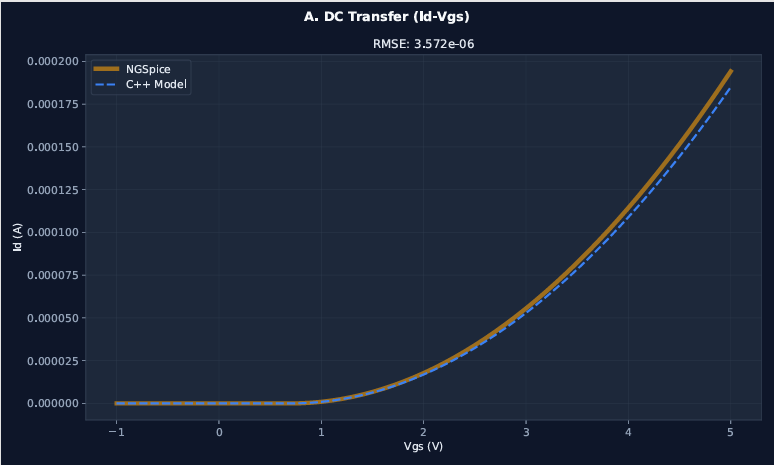
\includegraphics[width=\linewidth]{Figures/Ch5/MOSFET-1.png}
        \caption{MOSFET Characteristic Test 1.}
        \label{fig:mos_test_1}
    \end{minipage}\hfill
    \begin{minipage}{0.48\textwidth}
        \centering
        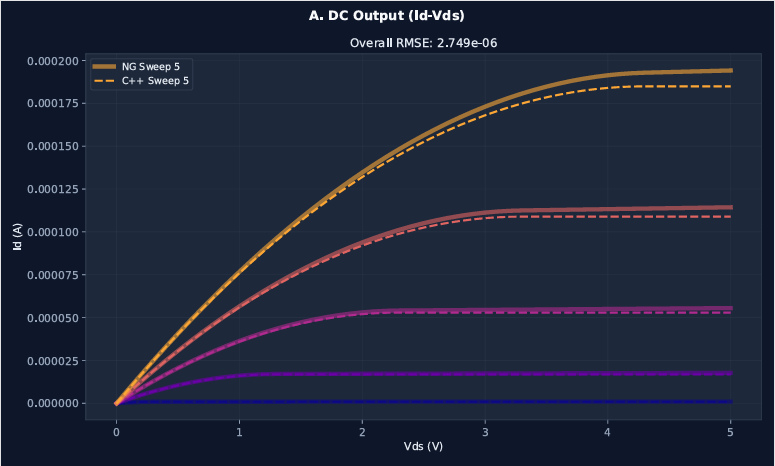
\includegraphics[width=\linewidth]{Figures/Ch5/MOSFET-2.png}
        \caption{MOSFET Characteristic Test 2.}
        \label{fig:mos_test_2}
    \end{minipage}
\end{figure}

\begin{figure}[H]
    \centering
    \begin{minipage}{0.48\textwidth}
        \centering
        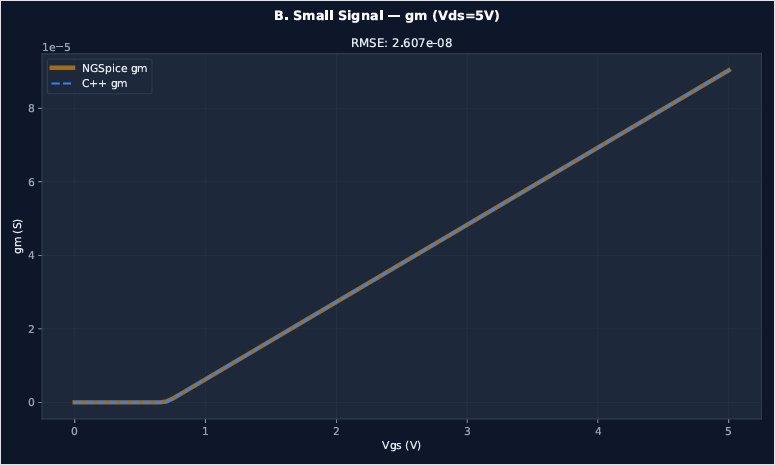
\includegraphics[width=\linewidth]{Figures/Ch5/MOSFET-3.png}
        \caption{MOSFET Characteristic Test 3.}
        \label{fig:mos_test_3}
    \end{minipage}\hfill
    \begin{minipage}{0.48\textwidth}
        \centering
        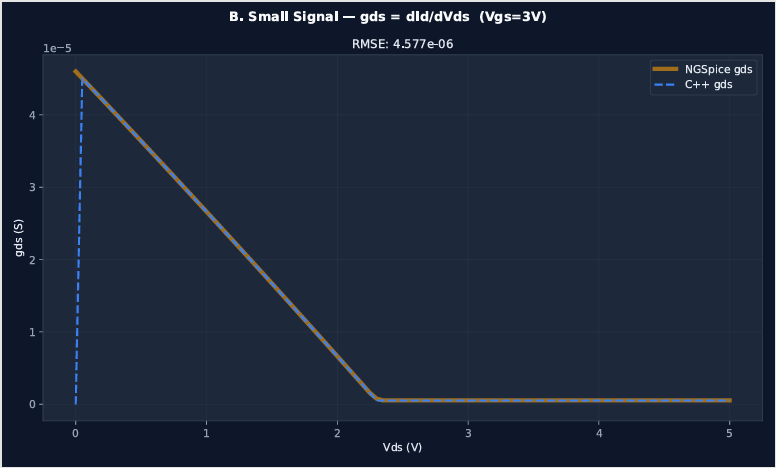
\includegraphics[width=\linewidth]{Figures/Ch5/MOSFET-4.png}
        \caption{MOSFET Characteristic Test 4.}
        \label{fig:mos_test_4}
    \end{minipage}
\end{figure}

\begin{figure}[H]
    \centering
    \begin{minipage}{0.48\textwidth}
        \centering
        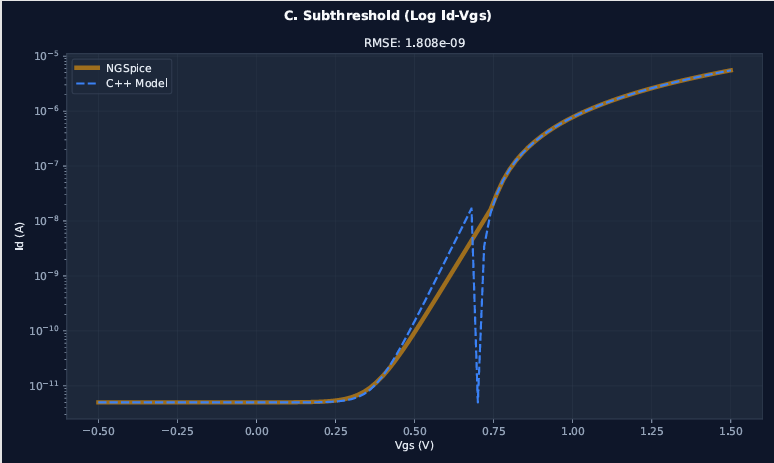
\includegraphics[width=\linewidth]{Figures/Ch5/MOSFET-5.png}
        \caption{MOSFET Characteristic Test 5.}
        \label{fig:mos_test_5}
    \end{minipage}\hfill
    \begin{minipage}{0.48\textwidth}
        \centering
        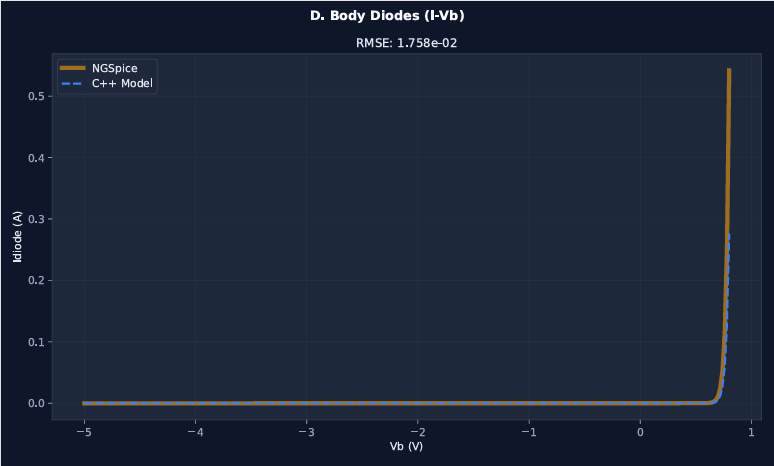
\includegraphics[width=\linewidth]{Figures/Ch5/MOSFET-6.png}
        \caption{MOSFET Characteristic Test 6.}
        \label{fig:mos_test_6}
    \end{minipage}
\end{figure}

\begin{figure}[H]
    \centering
    \begin{minipage}{0.48\textwidth}
        \centering
        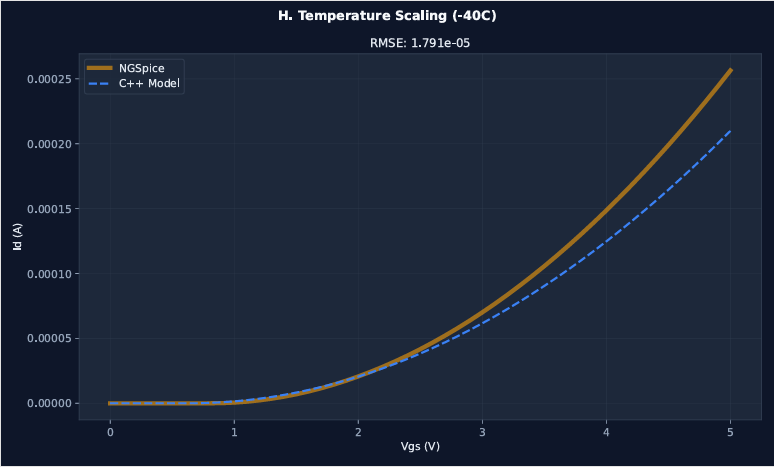
\includegraphics[width=\linewidth]{Figures/Ch5/MOSFET-7.png}
        \caption{MOSFET Characteristic Test 7.}
        \label{fig:mos_test_7}
    \end{minipage}\hfill
    \begin{minipage}{0.48\textwidth}
        \centering
        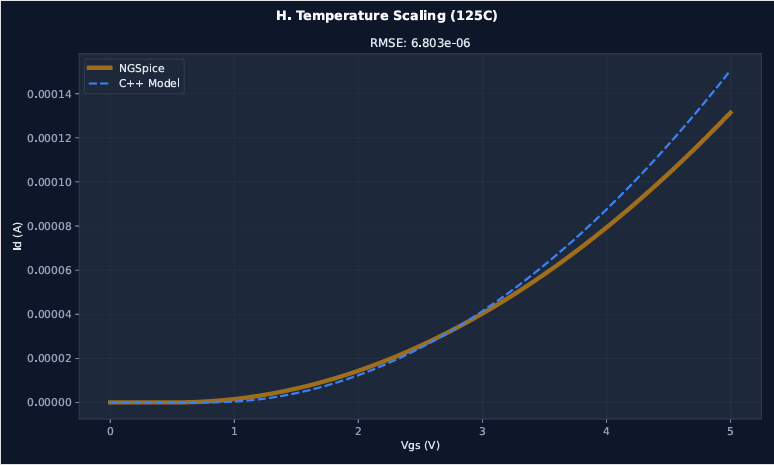
\includegraphics[width=\linewidth]{Figures/Ch5/MOSFET-8.png}
        \caption{MOSFET Characteristic Test 8.}
        \label{fig:mos_test_8}
    \end{minipage}
\end{figure}

\begin{figure}[H]
    \centering
    \begin{minipage}{0.48\textwidth}
        \centering
        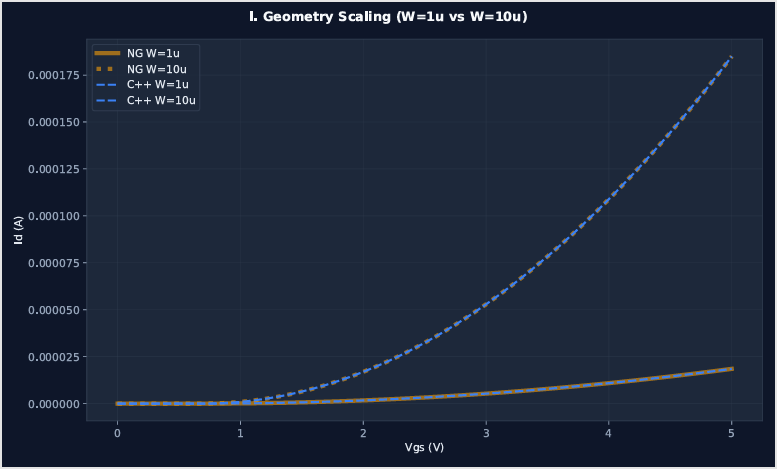
\includegraphics[width=\linewidth]{Figures/Ch5/MOSFET-9.png}
        \caption{MOSFET Characteristic Test 9.}
        \label{fig:mos_test_9}
    \end{minipage}\hfill
    \begin{minipage}{0.48\textwidth}
        \centering
        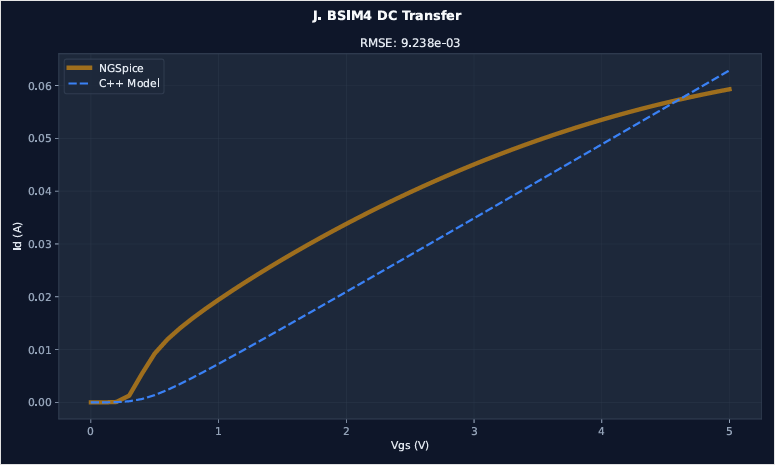
\includegraphics[width=\linewidth]{Figures/Ch5/MOSFET-10.png}
        \caption{MOSFET Characteristic Test 10.}
        \label{fig:mos_test_10}
    \end{minipage}
\end{figure}

\begin{figure}[H]
    \centering
    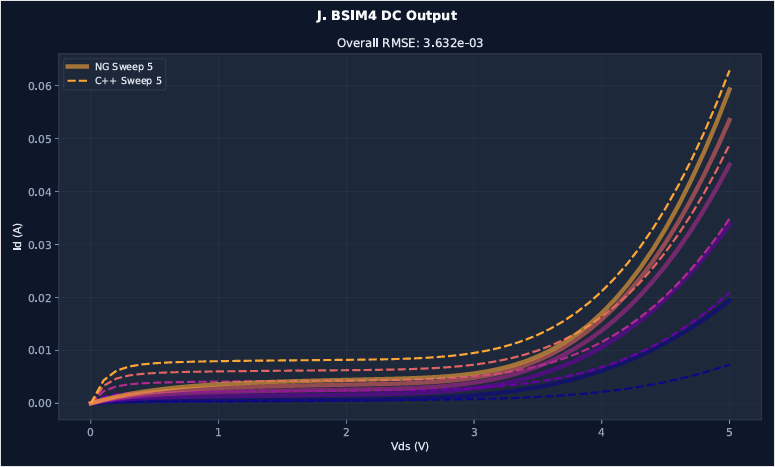
\includegraphics[width=0.6\textwidth]{Figures/Ch5/MOSFET-11.png}
    \caption{MOSFET Characteristic Test 11.}
    \label{fig:mos_test_11}
\end{figure}

\subsection{Bipolar Junction Transistor (BJT)}
BJT tests focus on the Ebers-Moll transport model, beta rolloff, Early effect, and high-frequency gain parameters.

\subsubsection{Internal C++ Unit Tests (Google Test)}
Google Test validates Gummel plots, high-current beta rolloff (IKF limit), and base resistance modulation ($R_b$):
\begin{itemize}
    \item \textbf{Gummel Characteristics:} Validates base and collector current separation across the forward bias range.
    \item \textbf{Beta Rolloff:} Confirms high-current beta rolloff ($IKF$) and output impedance modulation ($V_{af}$).
    \item \textbf{Junction Capacitance:} Verifies $C_{be}, C_{bc}$, and extrinsic $C_{bx}$ profiles.
    \item \textbf{Substrate Branch:} Validates substrate junction currents and capacitances.
\end{itemize}

\subsubsection{NGSpice Verification}
Figures~\ref{fig:bjt_test_1} to \ref{fig:bjt_test_4} display the Gummel plots, output characteristics, base/collector junction capacitances, and transient common-emitter amplifier waveforms compared against NGSpice.

\begin{figure}[H]
    \centering
    \begin{minipage}{0.48\textwidth}
        \centering
        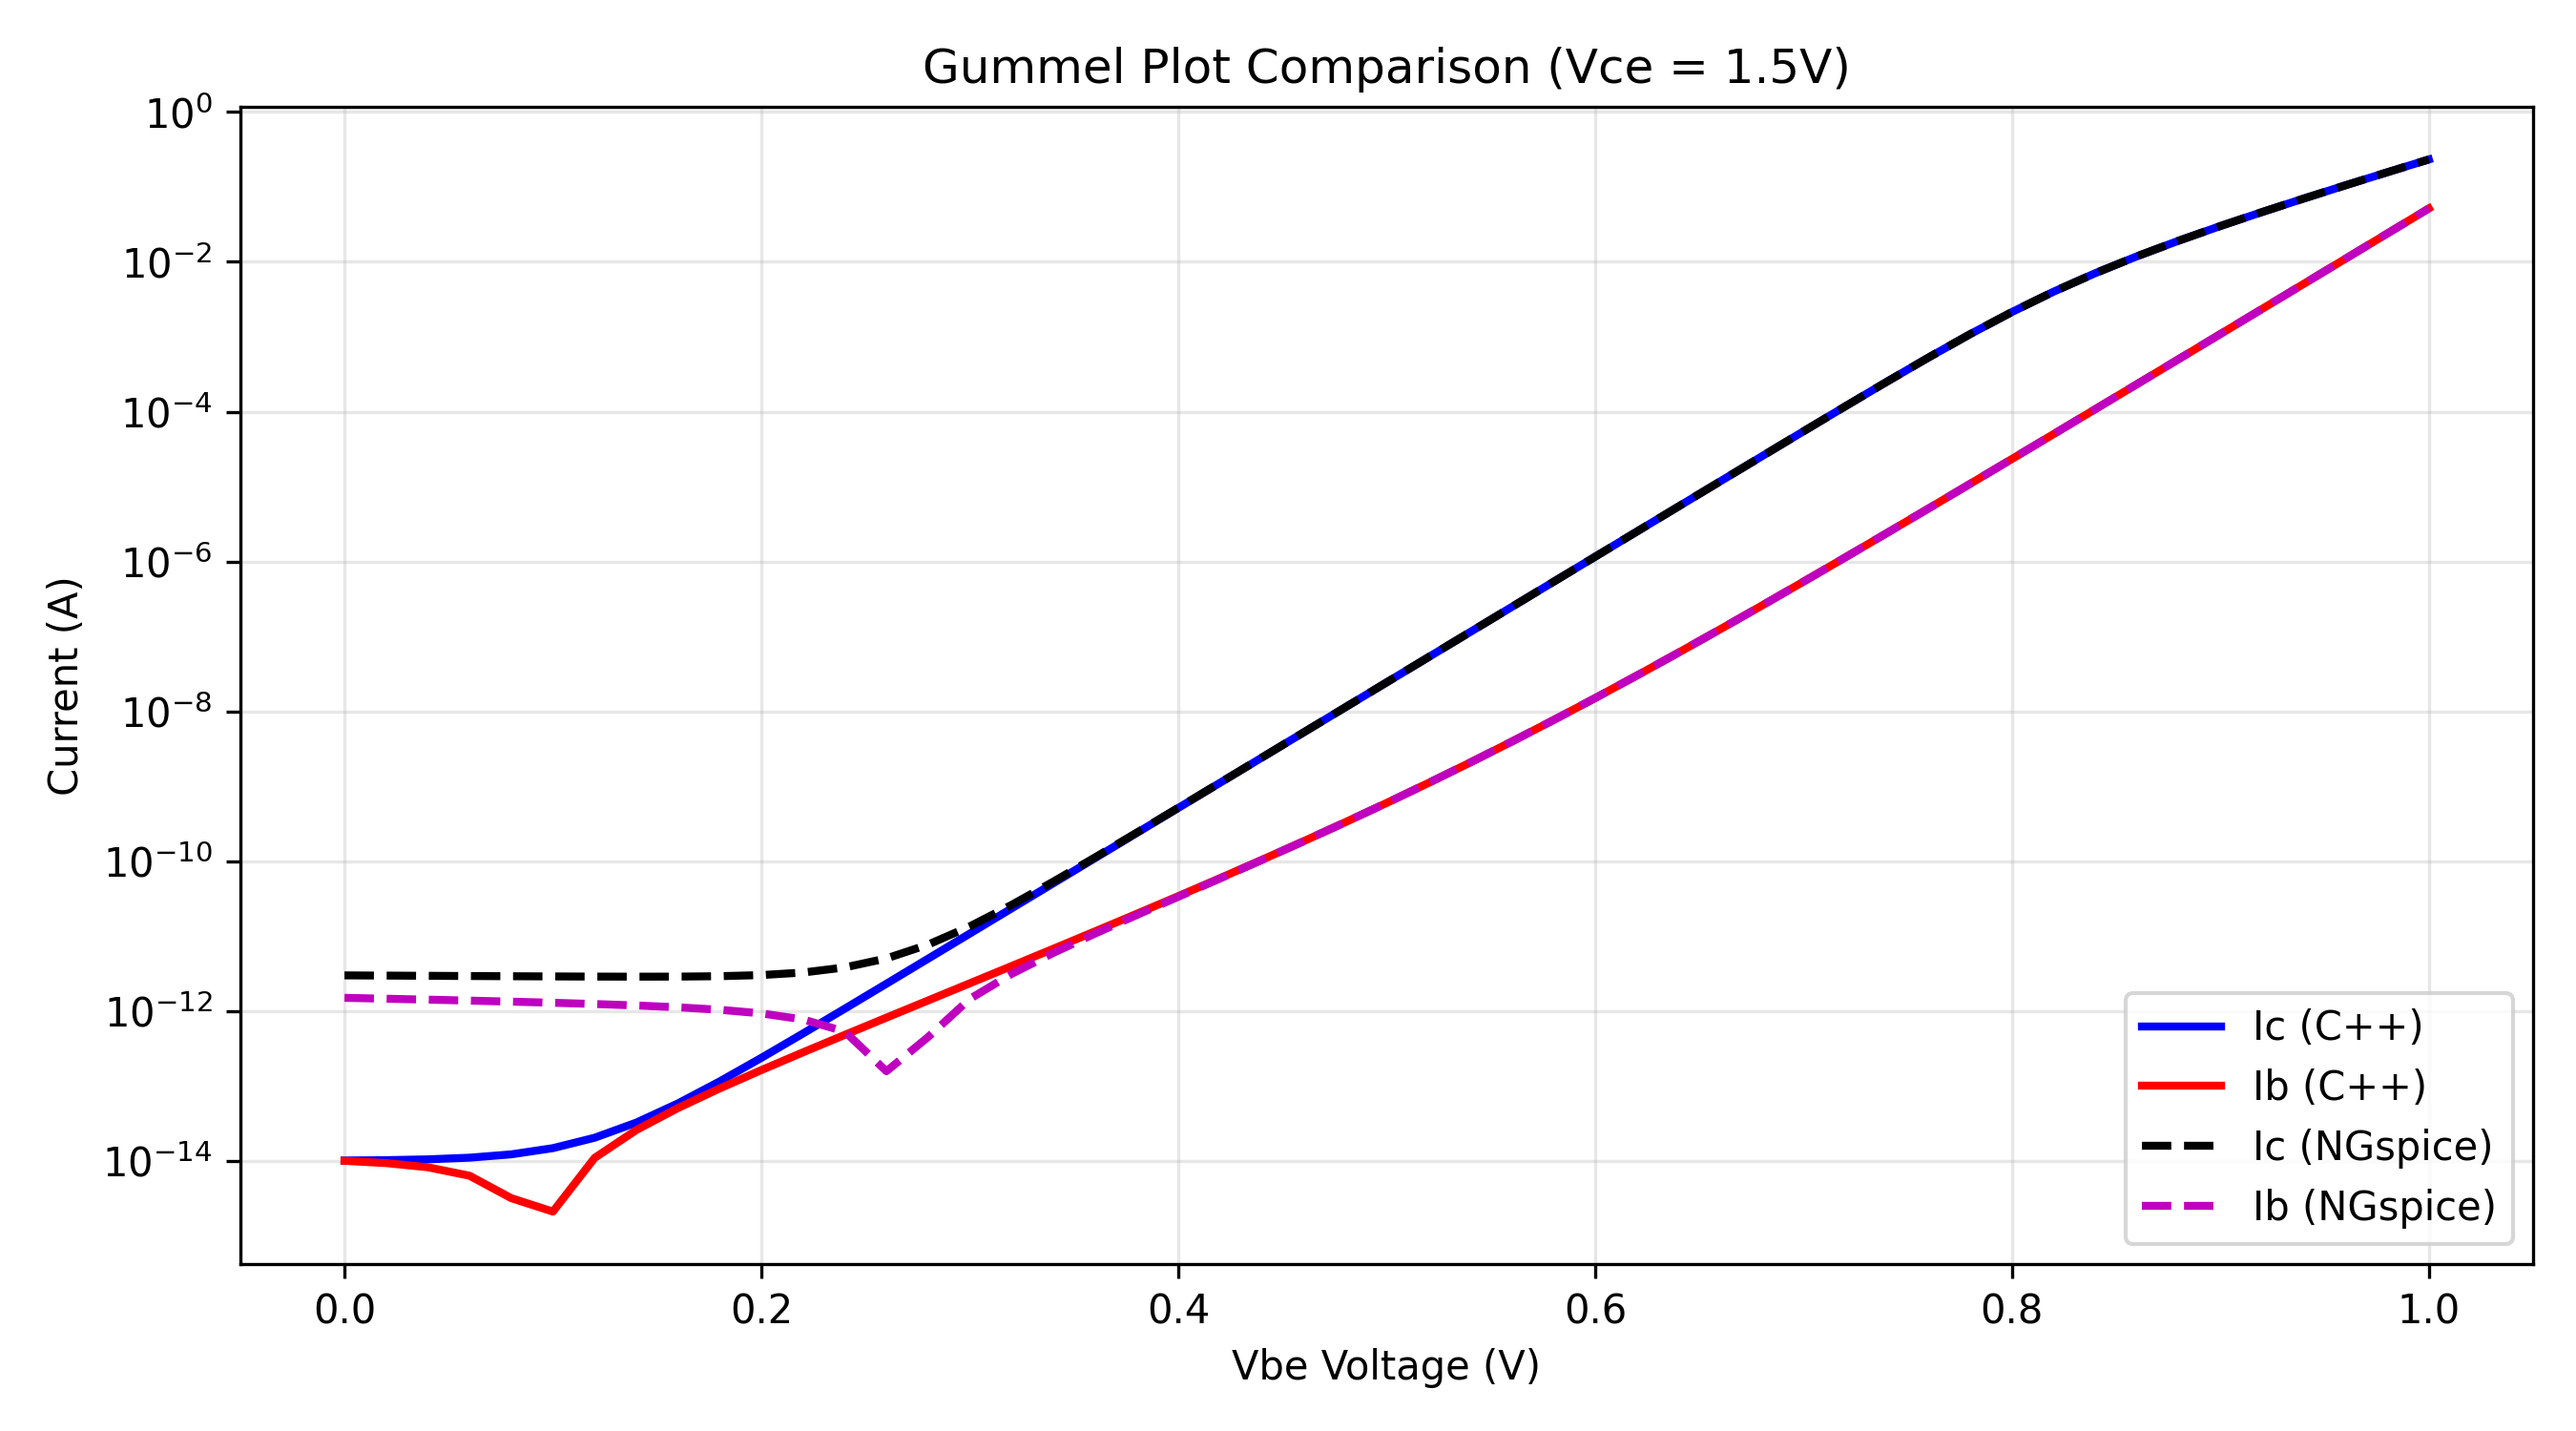
\includegraphics[width=\linewidth]{Figures/Ch5/BJT-1.png}
        \caption{BJT Gummel Plot ($I_c, I_b$ vs. $V_{be}$).}
        \label{fig:bjt_test_1}
    \end{minipage}\hfill
    \begin{minipage}{0.48\textwidth}
        \centering
        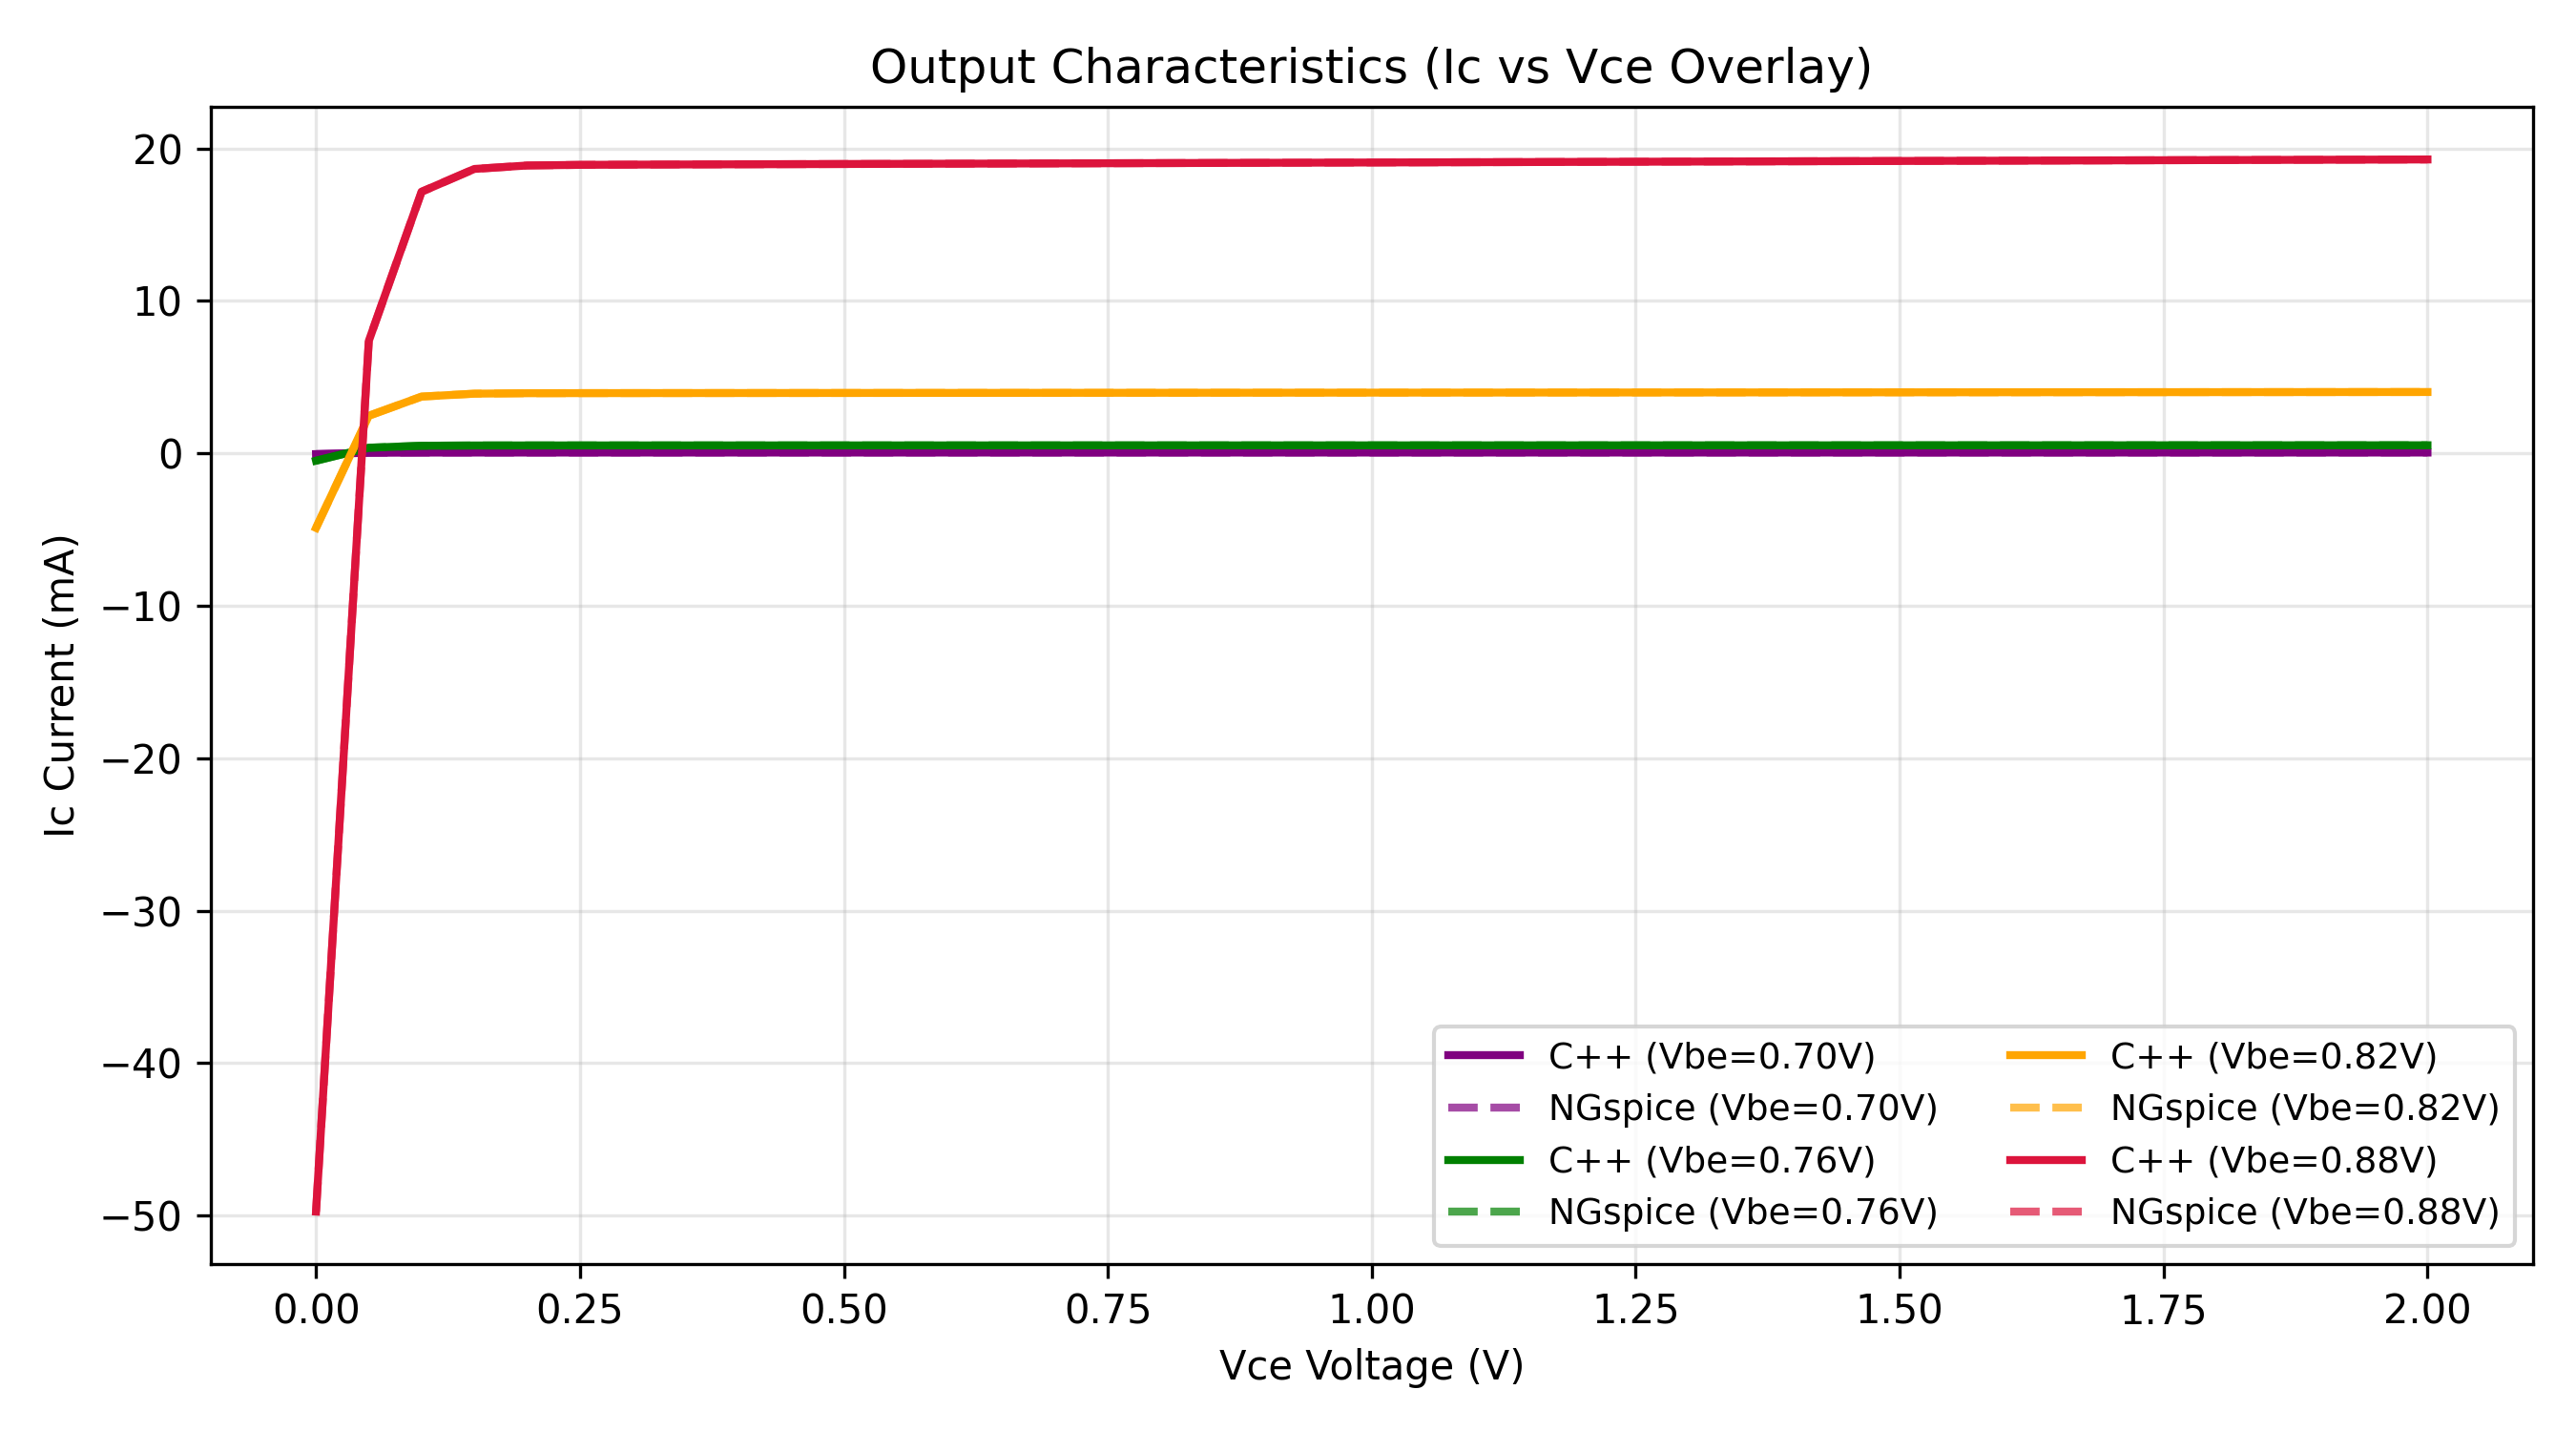
\includegraphics[width=\linewidth]{Figures/Ch5/BJT-2.png}
        \caption{BJT Output Characteristics ($I_c$ vs. $V_{ce}$).}
        \label{fig:bjt_test_2}
    \end{minipage}
\end{figure}

\begin{figure}[H]
    \centering
    \begin{minipage}{0.48\textwidth}
        \centering
        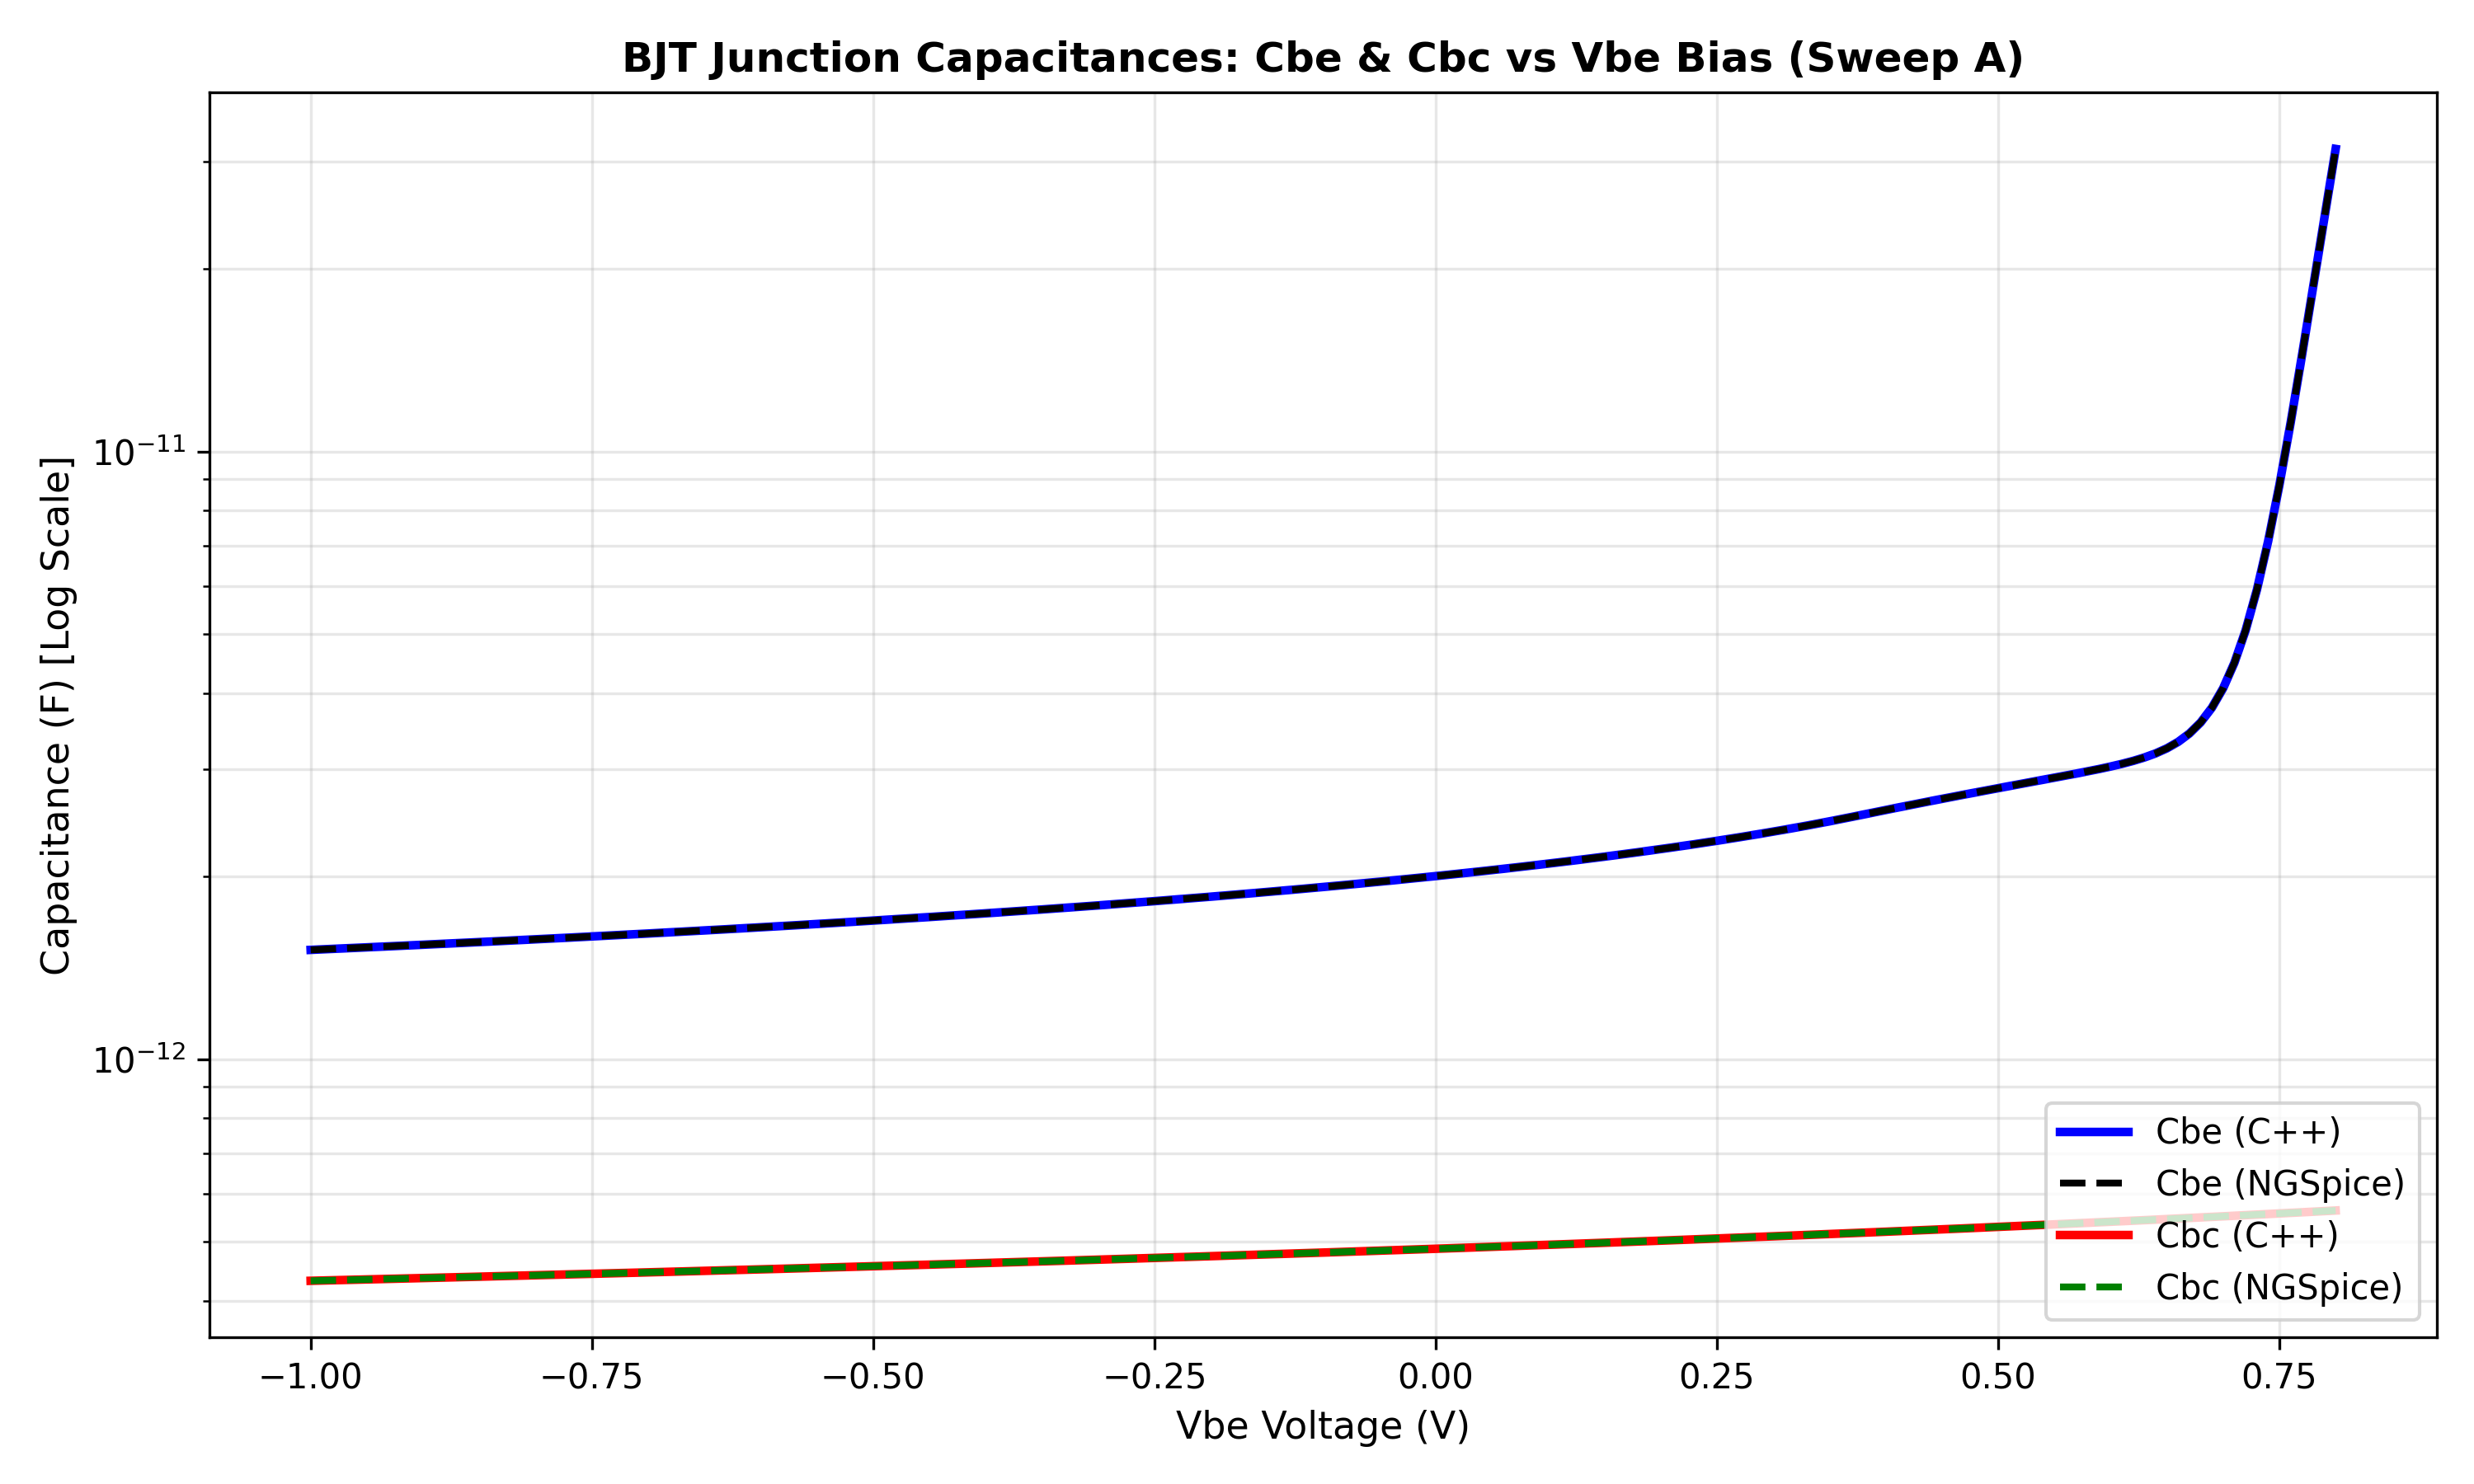
\includegraphics[width=\linewidth]{Figures/Ch5/BJT-3.png}
        \caption{BJT Junction Capacitances ($C_{be}, C_{bc}$).}
        \label{fig:bjt_test_3}
    \end{minipage}\hfill
    \begin{minipage}{0.48\textwidth}
        \centering
        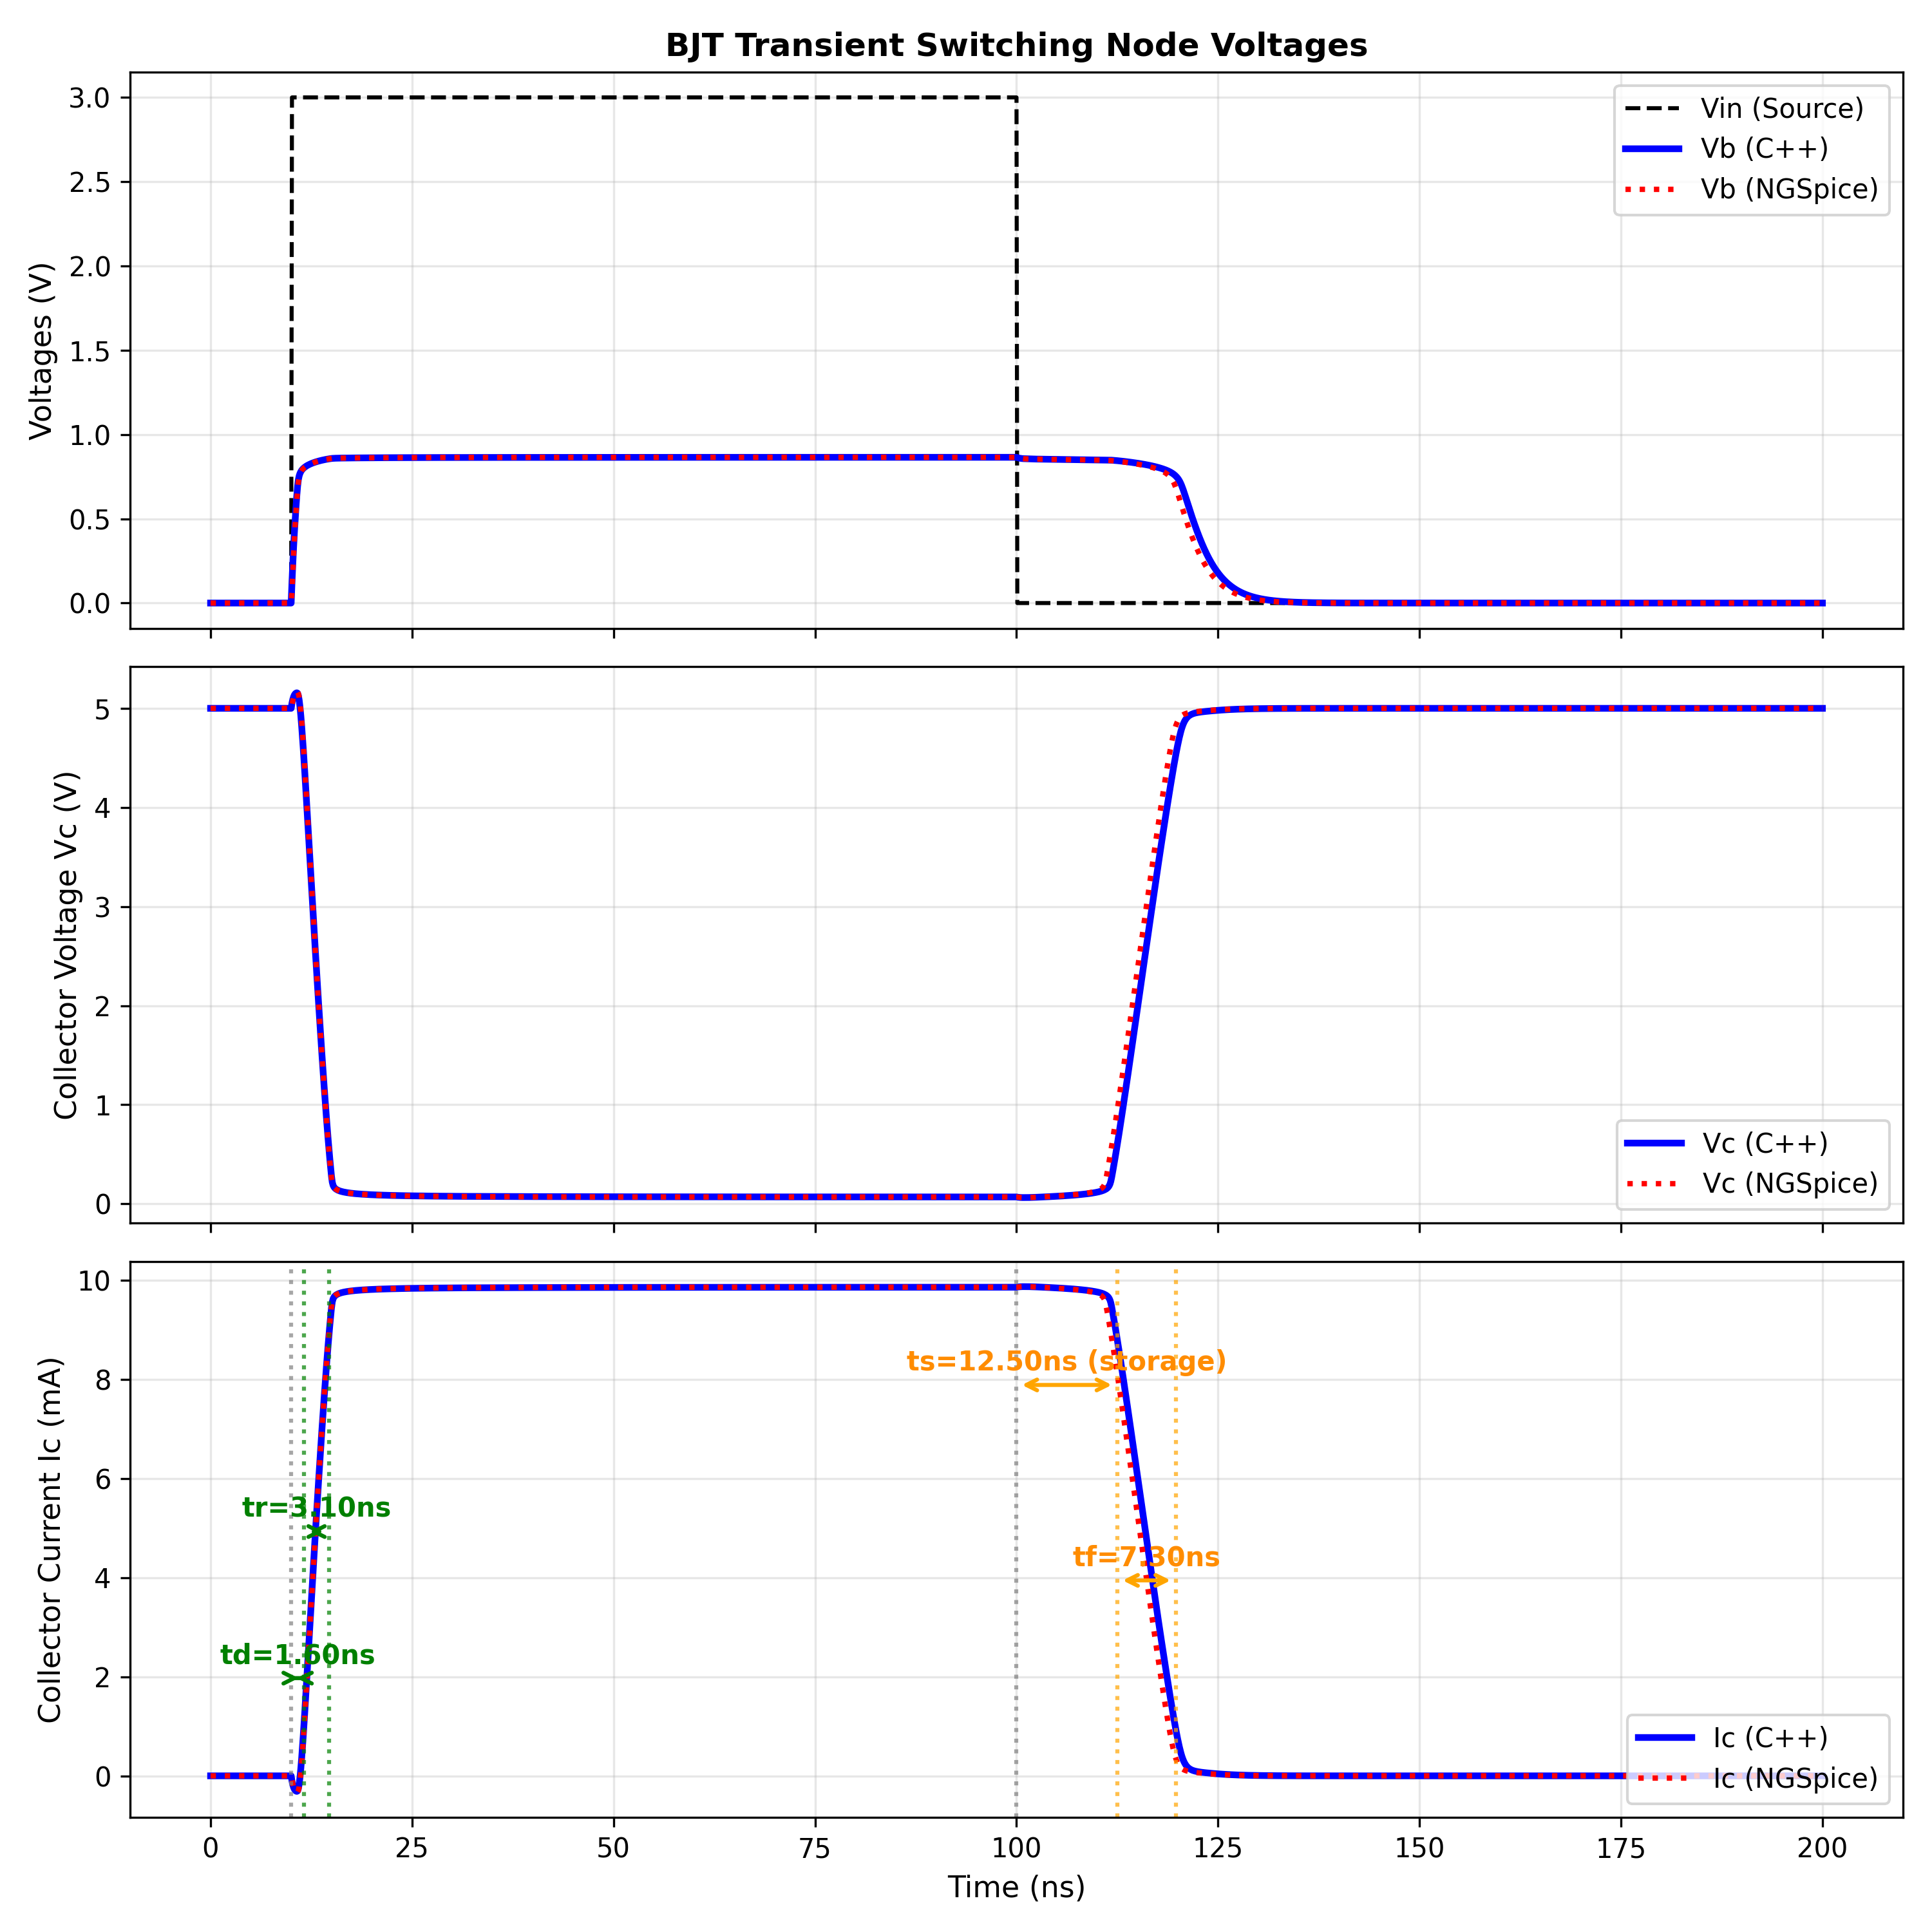
\includegraphics[width=\linewidth]{Figures/Ch5/BJT-4.png}
        \caption{BJT Transient Amplifier Waveforms.}
        \label{fig:bjt_test_4}
    \end{minipage}
\end{figure}

\subsection{Independent Voltage Source (VS)}
The independent voltage source unit tests verify the waveform generation capabilities (DC, PULSE, SIN, EXP, PWL) and the correct MNA branch stamping and current retrieval.

\subsubsection{Internal C++ Unit Tests (Google Test)}
An extensive suite of Google Test cases validates the implementation details:
\begin{itemize}
    \item \textbf{Waveform Generation:} Tests DC and PULSE waveform evaluation using \texttt{updateState()} to confirm proper simulation-time tracking and instantaneous voltage calculation.
    \item \textbf{PWL Breakpoint Sorting:} Confirms that piecewise-linear (PWL) source timestamp breakpoints are accurately extracted, sorted, and correctly reported to the transient stepping engine.
    \item \textbf{MNA Stamping:} Verifies that the conductance matrix $G$ strictly holds $+1$ and $-1$ at the correct branch/node intersections, and that the $RHS$ vector holds the accurate instantaneous voltage value at the appropriate branch index.
\end{itemize}

\subsubsection{NGSpice Verification}
Figures~\ref{fig:vs_test_1} to \ref{fig:vs_test_3} illustrate the NGSpice verification plots for the Independent Voltage Source. The figures confirm the successful generation of complex transient waveforms and their accurate boundary-condition enforcement within the MNA equations.

\begin{figure}[H]
    \centering
    \begin{minipage}{0.48\textwidth}
        \centering
        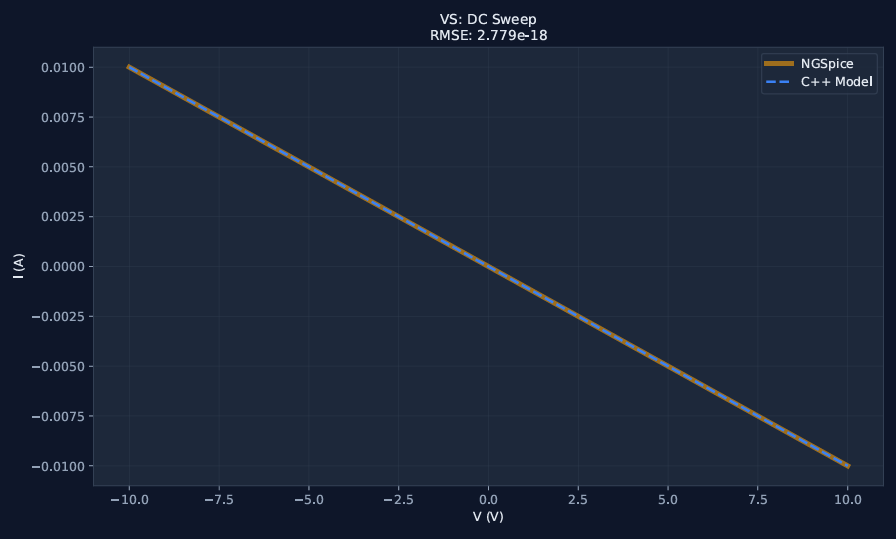
\includegraphics[width=\linewidth]{Figures/Ch5/VS-1.png}
        \caption{Voltage Source Transient Waveform Test 1.}
        \label{fig:vs_test_1}
    \end{minipage}\hfill
    \begin{minipage}{0.48\textwidth}
        \centering
        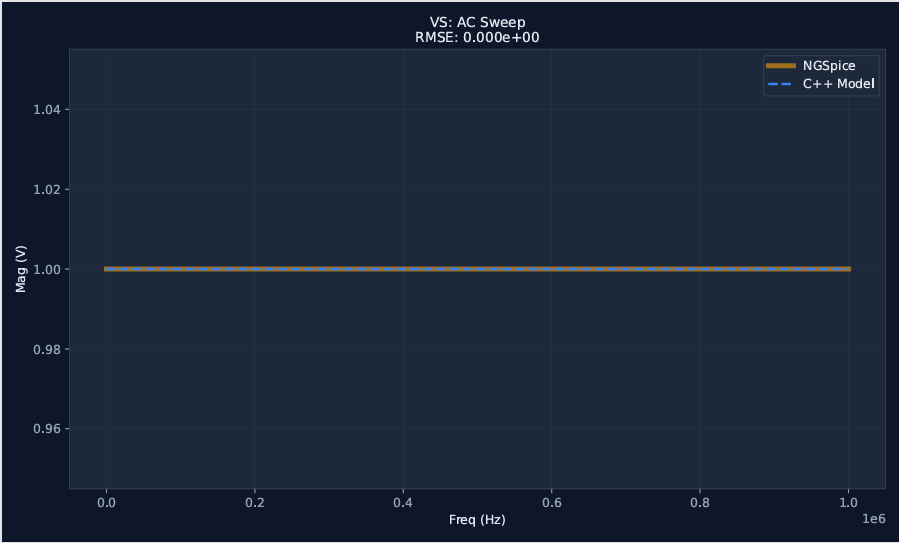
\includegraphics[width=\linewidth]{Figures/Ch5/VS-2.png}
        \caption{Voltage Source Transient Waveform Test 2.}
        \label{fig:vs_test_2}
    \end{minipage}
\end{figure}

\begin{figure}[H]
    \centering
    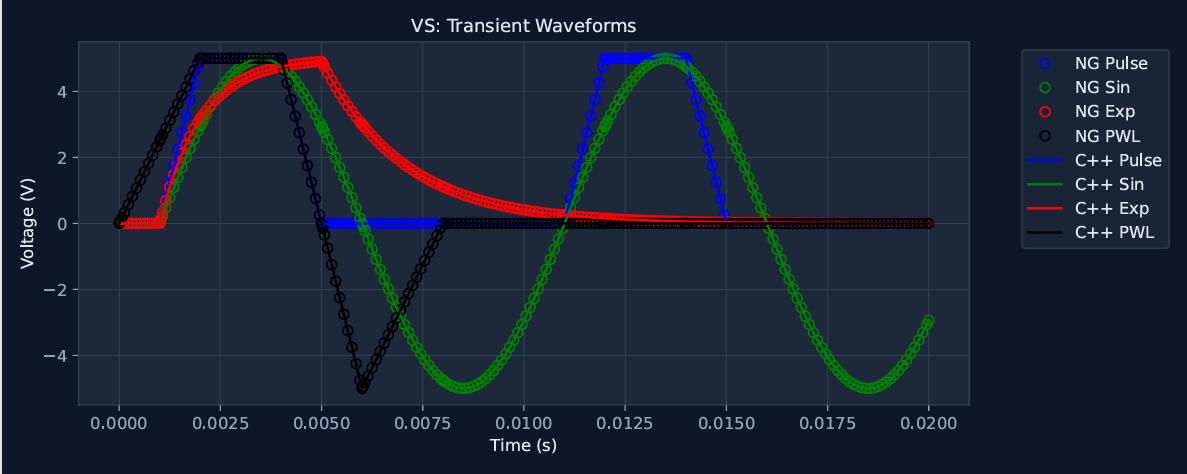
\includegraphics[width=0.6\textwidth]{Figures/Ch5/VS-3.png}
    \caption{Voltage Source Transient Waveform Test 3.}
    \label{fig:vs_test_3}
\end{figure}

\subsection{Independent Current Source (CS)}
The independent current source unit tests check the waveform evaluation and RHS current injection paths.

\subsubsection{Internal C++ Unit Tests (Google Test)}
Google Test cases verify the current source's exact functional behavior:
\begin{itemize}
    \item \textbf{Waveform Evaluation:} Tests DC current retrieval and state updates using \texttt{updateState()} to ensure precise simulation-time tracking of injected currents.
    \item \textbf{PWL Breakpoint Sorting:} Confirms that piecewise-linear (PWL) time-value coordinate pairs are properly accumulated, sorted, and correctly reported as temporal breakpoints to the transient solver.
    \item \textbf{MNA RHS Injection:} Verifies that conventional source current is perfectly injected into the MNA RHS vector, strictly adhering to KCL by subtracting from the positive terminal index and adding to the negative terminal index.
\end{itemize}

\subsubsection{NGSpice Verification}
Figures~\ref{fig:cs_test_1} to \ref{fig:cs_test_3} illustrate the NGSpice verification plots for the Independent Current Source. The figures confirm the successful generation of continuous and discontinuous transient current waveforms and their correct boundary enforcement across resistive or reactive loads within the MNA solver.

\begin{figure}[H]
    \centering
    \begin{minipage}{0.48\textwidth}
        \centering
        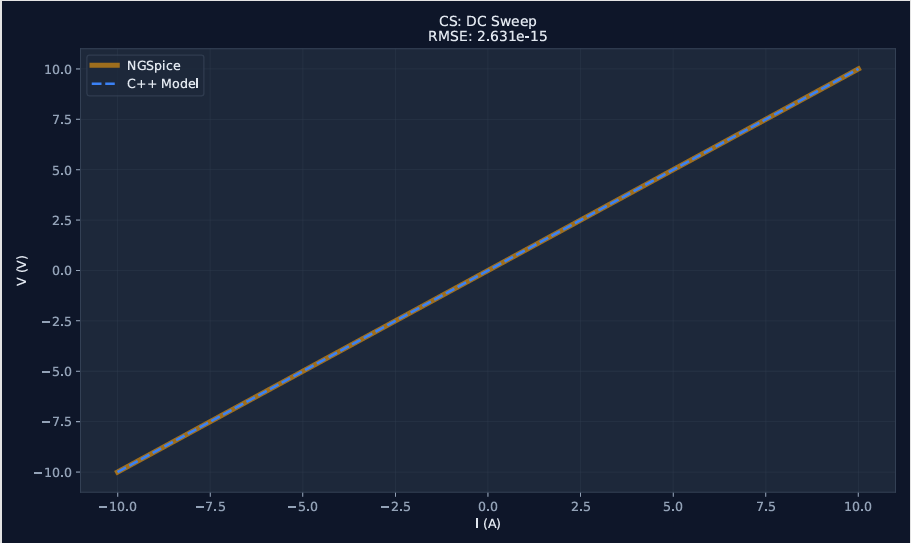
\includegraphics[width=\linewidth]{Figures/Ch5/CS-1.png}
        \caption{Current Source Transient Waveform Test 1.}
        \label{fig:cs_test_1}
    \end{minipage}\hfill
    \begin{minipage}{0.48\textwidth}
        \centering
        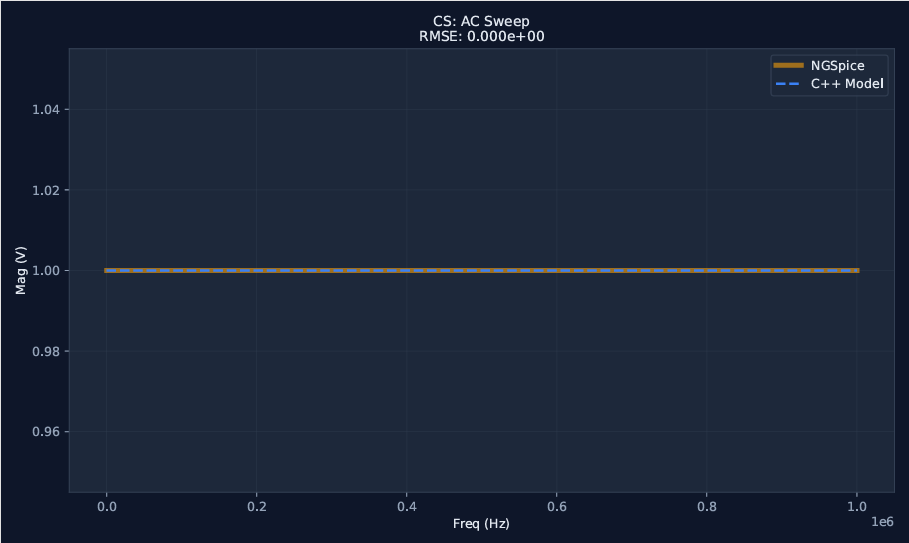
\includegraphics[width=\linewidth]{Figures/Ch5/CS-2.png}
        \caption{Current Source Transient Waveform Test 2.}
        \label{fig:cs_test_2}
    \end{minipage}
\end{figure}

\begin{figure}[H]
    \centering
    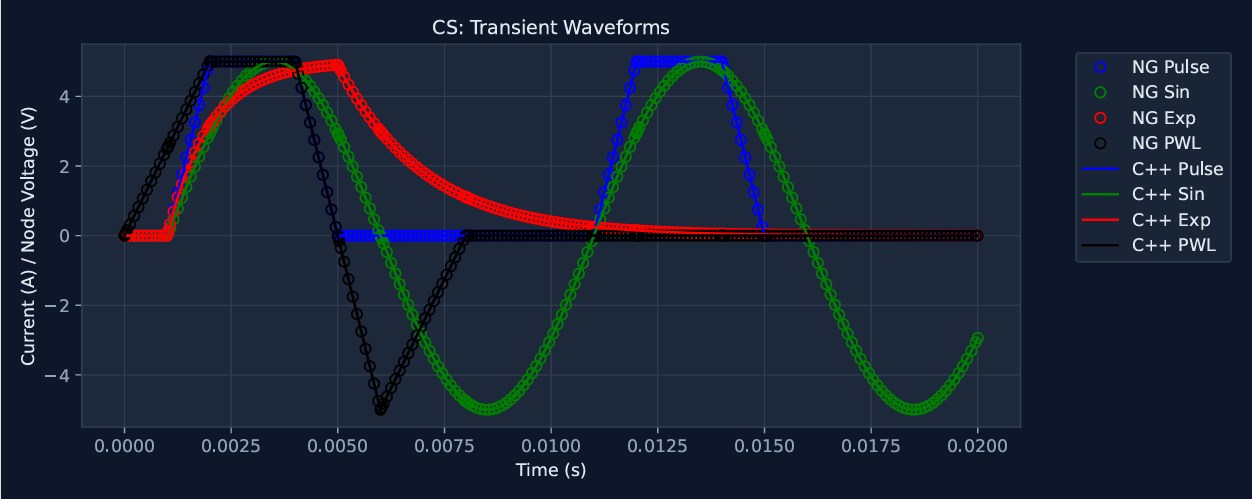
\includegraphics[width=0.6\textwidth]{Figures/Ch5/CS-3.png}
    \caption{Current Source Transient Waveform Test 3.}
    \label{fig:cs_test_3}
\end{figure}

\subsection{Voltage-Controlled Current Source (VCCS)}
The VCCS unit tests verify linear transconductance coupling and correct MNA matrix integration.

\subsubsection{Internal C++ Unit Tests}
The C++ testing framework validates the VCCS through an integrated matrix solver sweep:
\begin{itemize}
    \item \textbf{MNA Stamping Layout:} Verifies that the controlling nodes ($p_{ctrl}, n_{ctrl}$) and output nodes ($p, n$) are correctly stamped with the transconductance gain $+g_m$ and $-g_m$ across their Cartesian intersections in the conductance matrix $G$.
    \item \textbf{Linear Sweep Simulation:} Confirms that the output current dynamically tracks the transconductance times the controlling differential voltage during a simulated DC voltage sweep by solving the linear system via Gaussian elimination.
\end{itemize}

\subsubsection{NGSpice Verification}
Figures~\ref{fig:vccs_test_1} to \ref{fig:vccs_test_3} illustrate the NGSpice verification plots for the VCCS. The C++ generated DC sweep data is compared directly against NGSpice output, validating the perfect tracking of the transconductance transfer function.

\begin{figure}[H]
    \centering
    \begin{minipage}{0.48\textwidth}
        \centering
        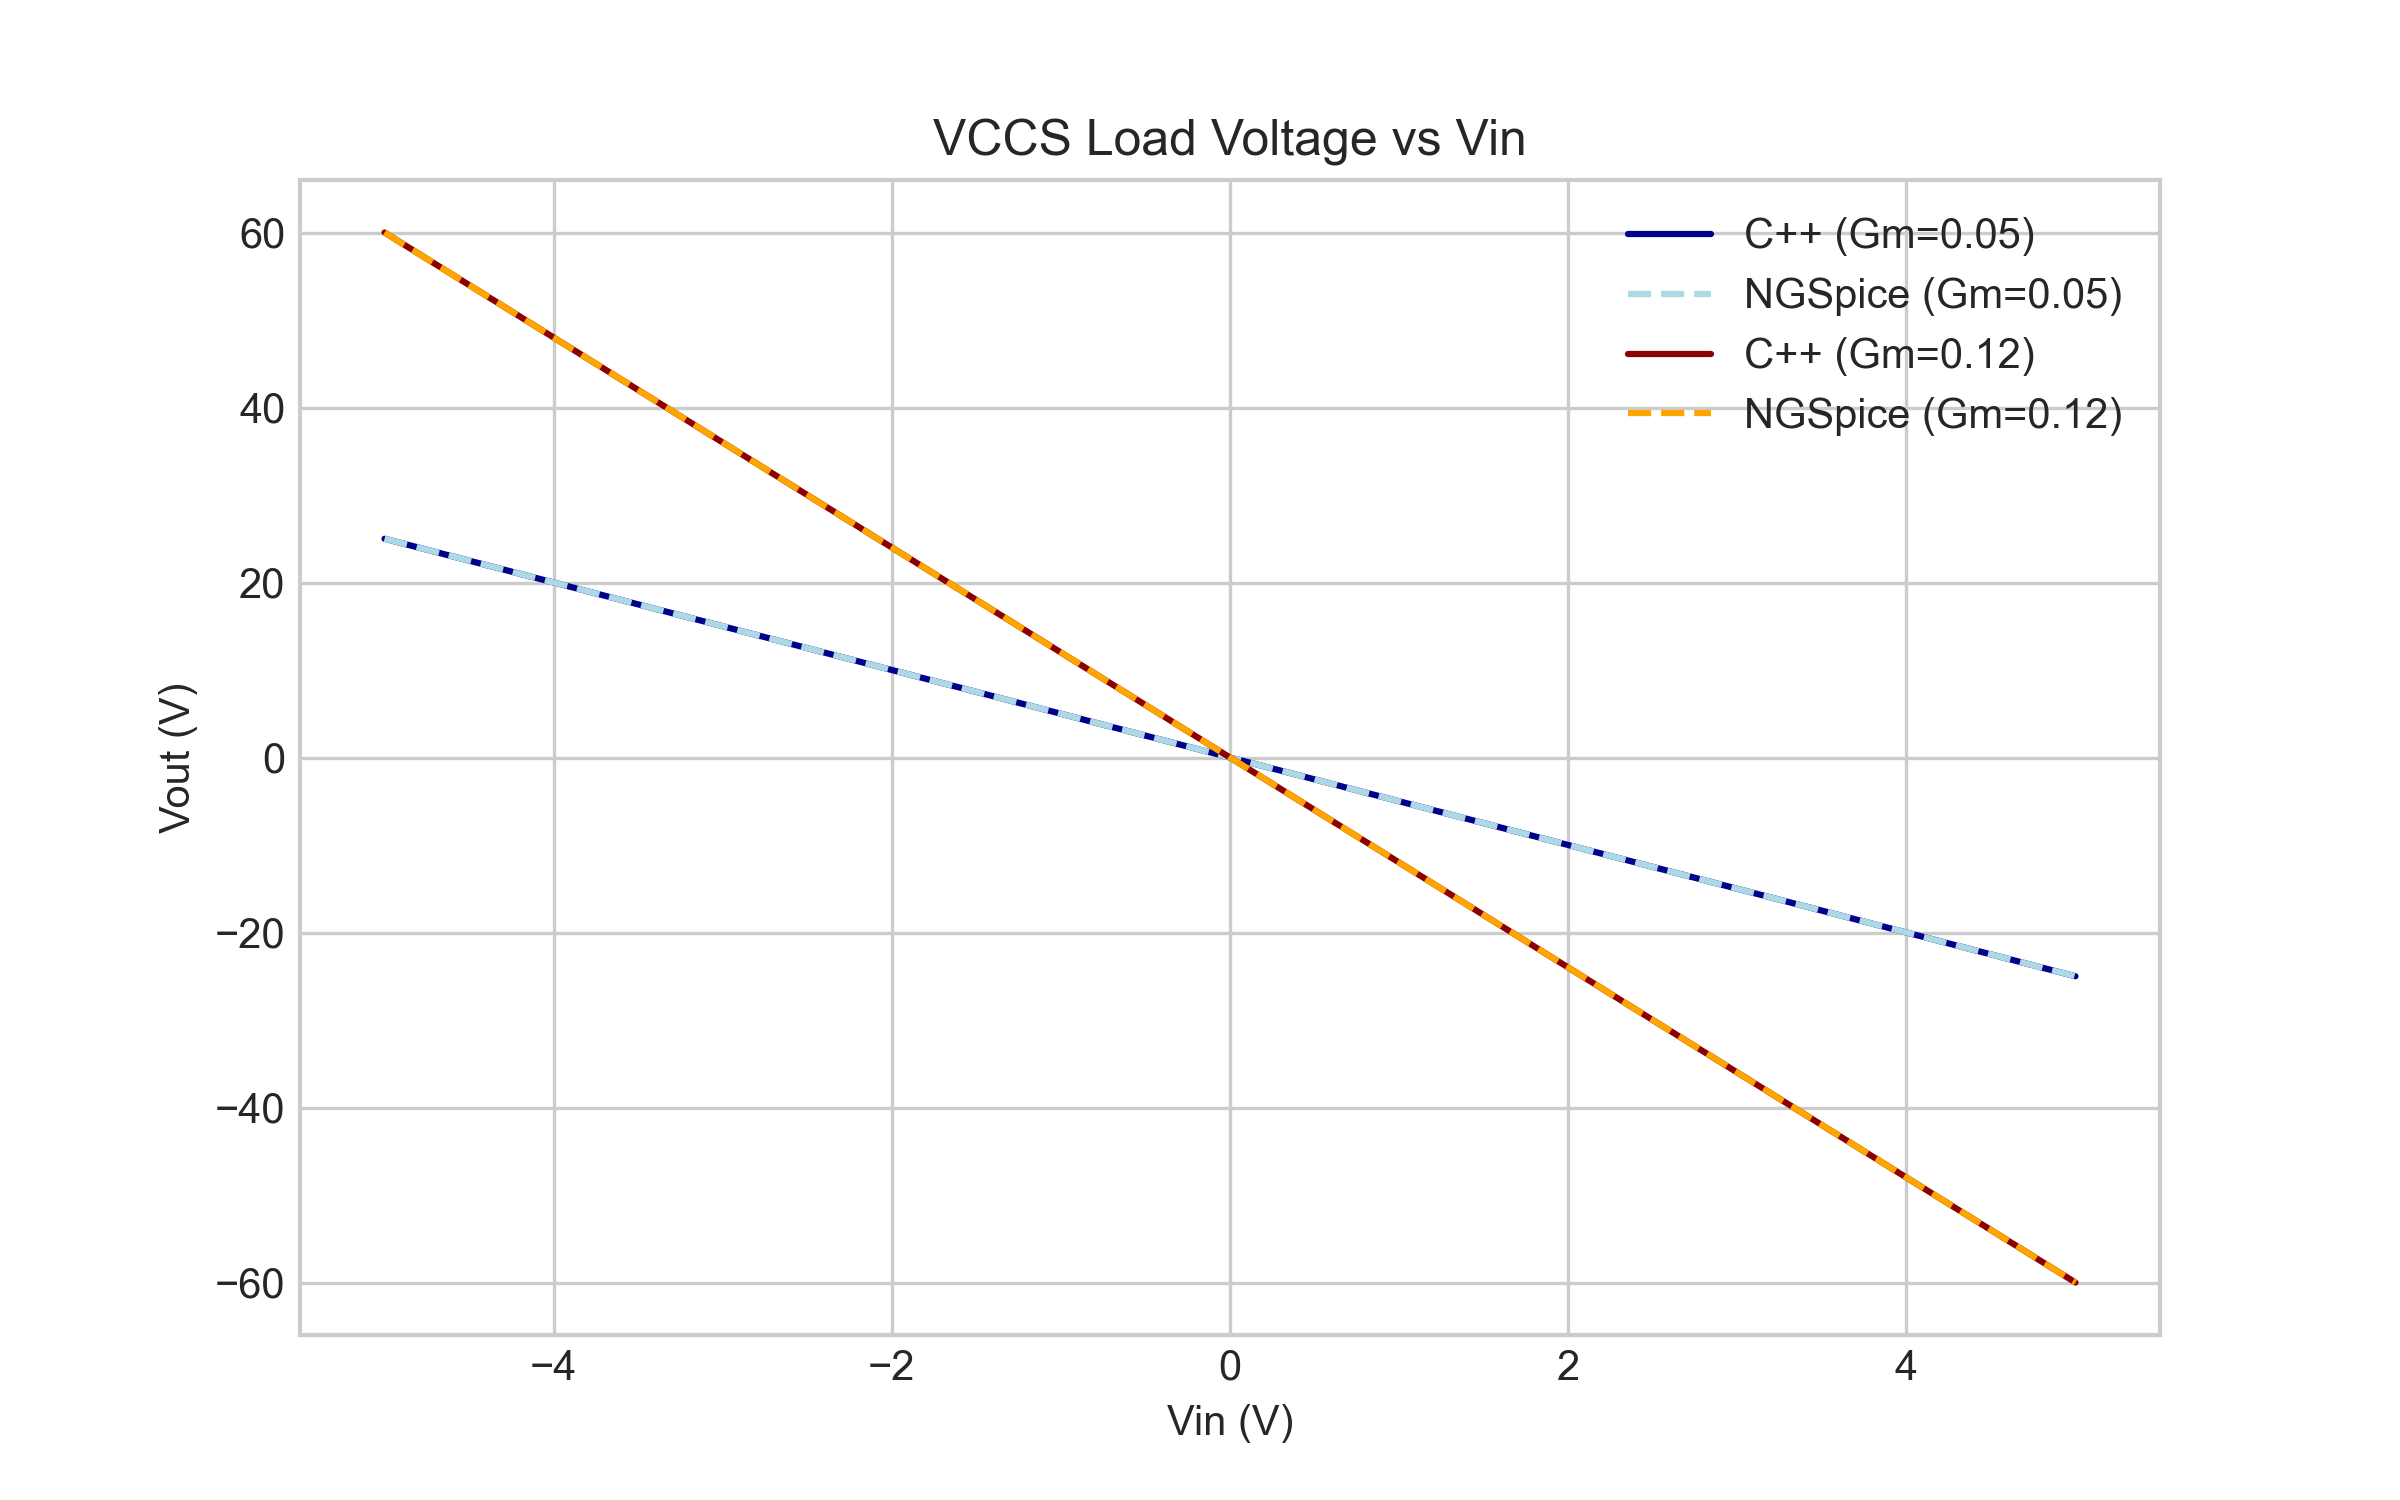
\includegraphics[width=\linewidth]{Figures/Ch5/vccs_1.png}
        \caption{VCCS Transfer Characteristic Test 1.}
        \label{fig:vccs_test_1}
    \end{minipage}\hfill
    \begin{minipage}{0.48\textwidth}
        \centering
        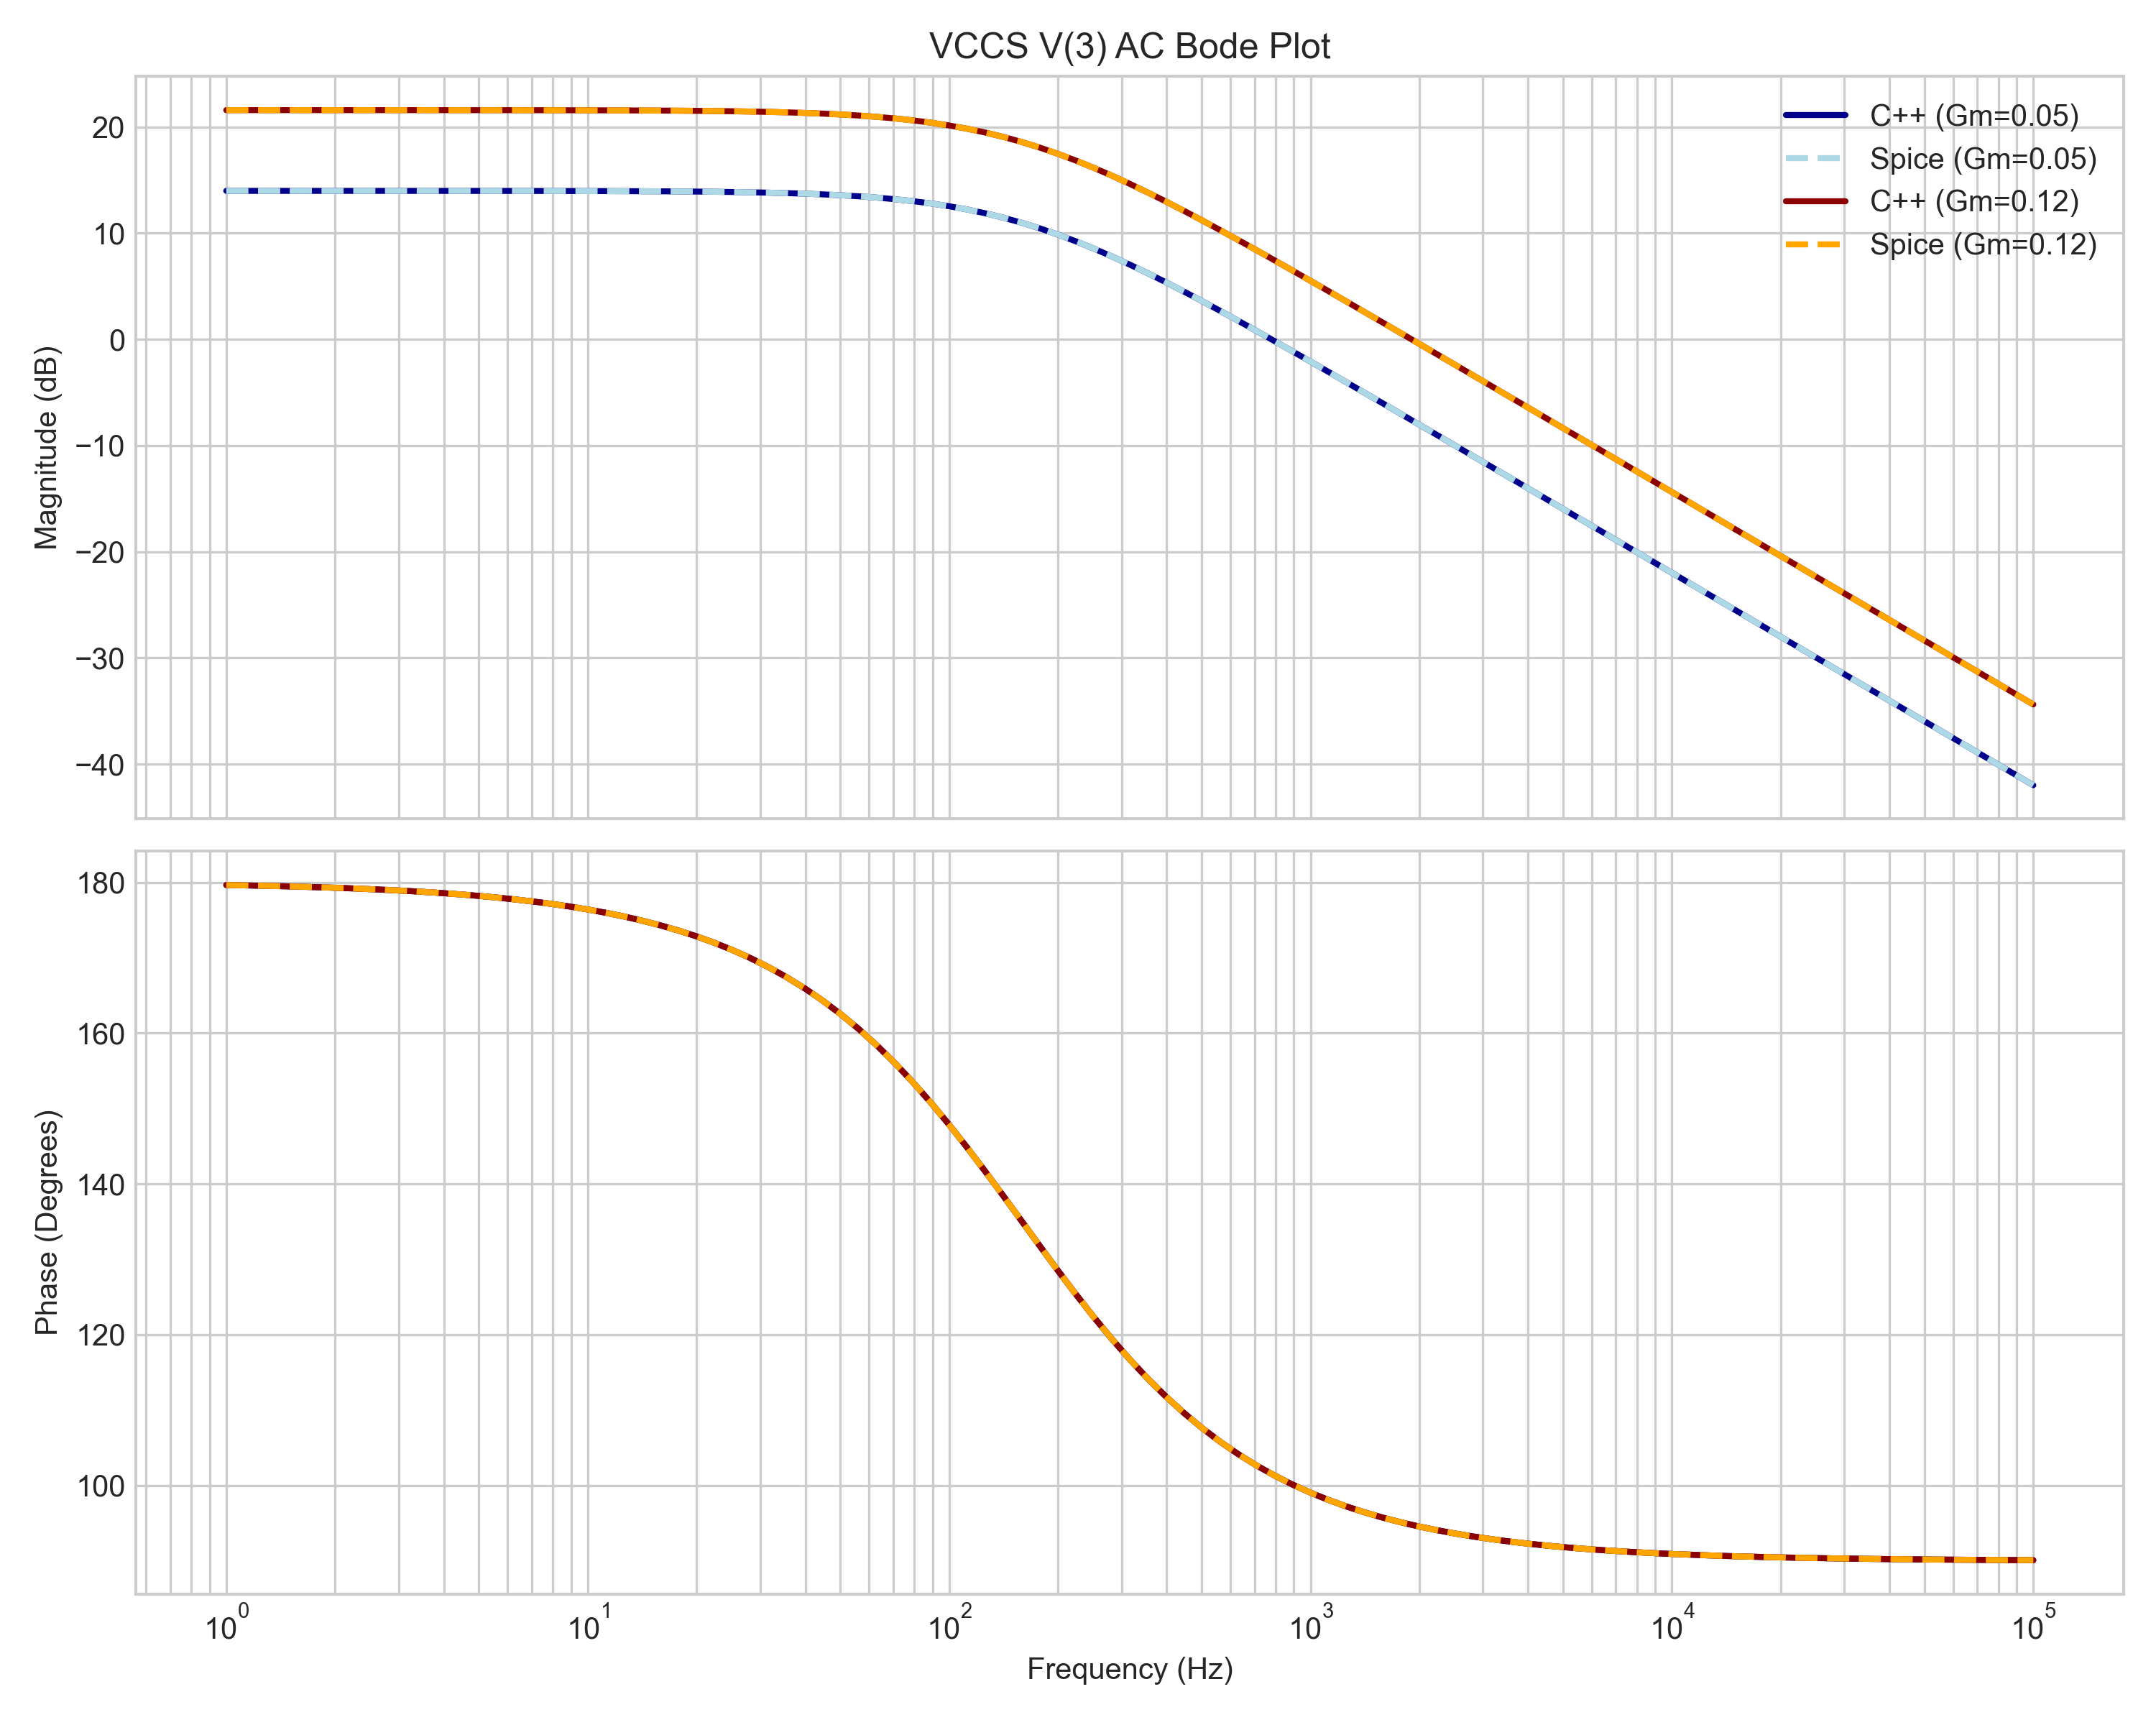
\includegraphics[width=\linewidth]{Figures/Ch5/vccs_2.png}
        \caption{VCCS Transfer Characteristic Test 2.}
        \label{fig:vccs_test_2}
    \end{minipage}
\end{figure}

\begin{figure}[H]
    \centering
    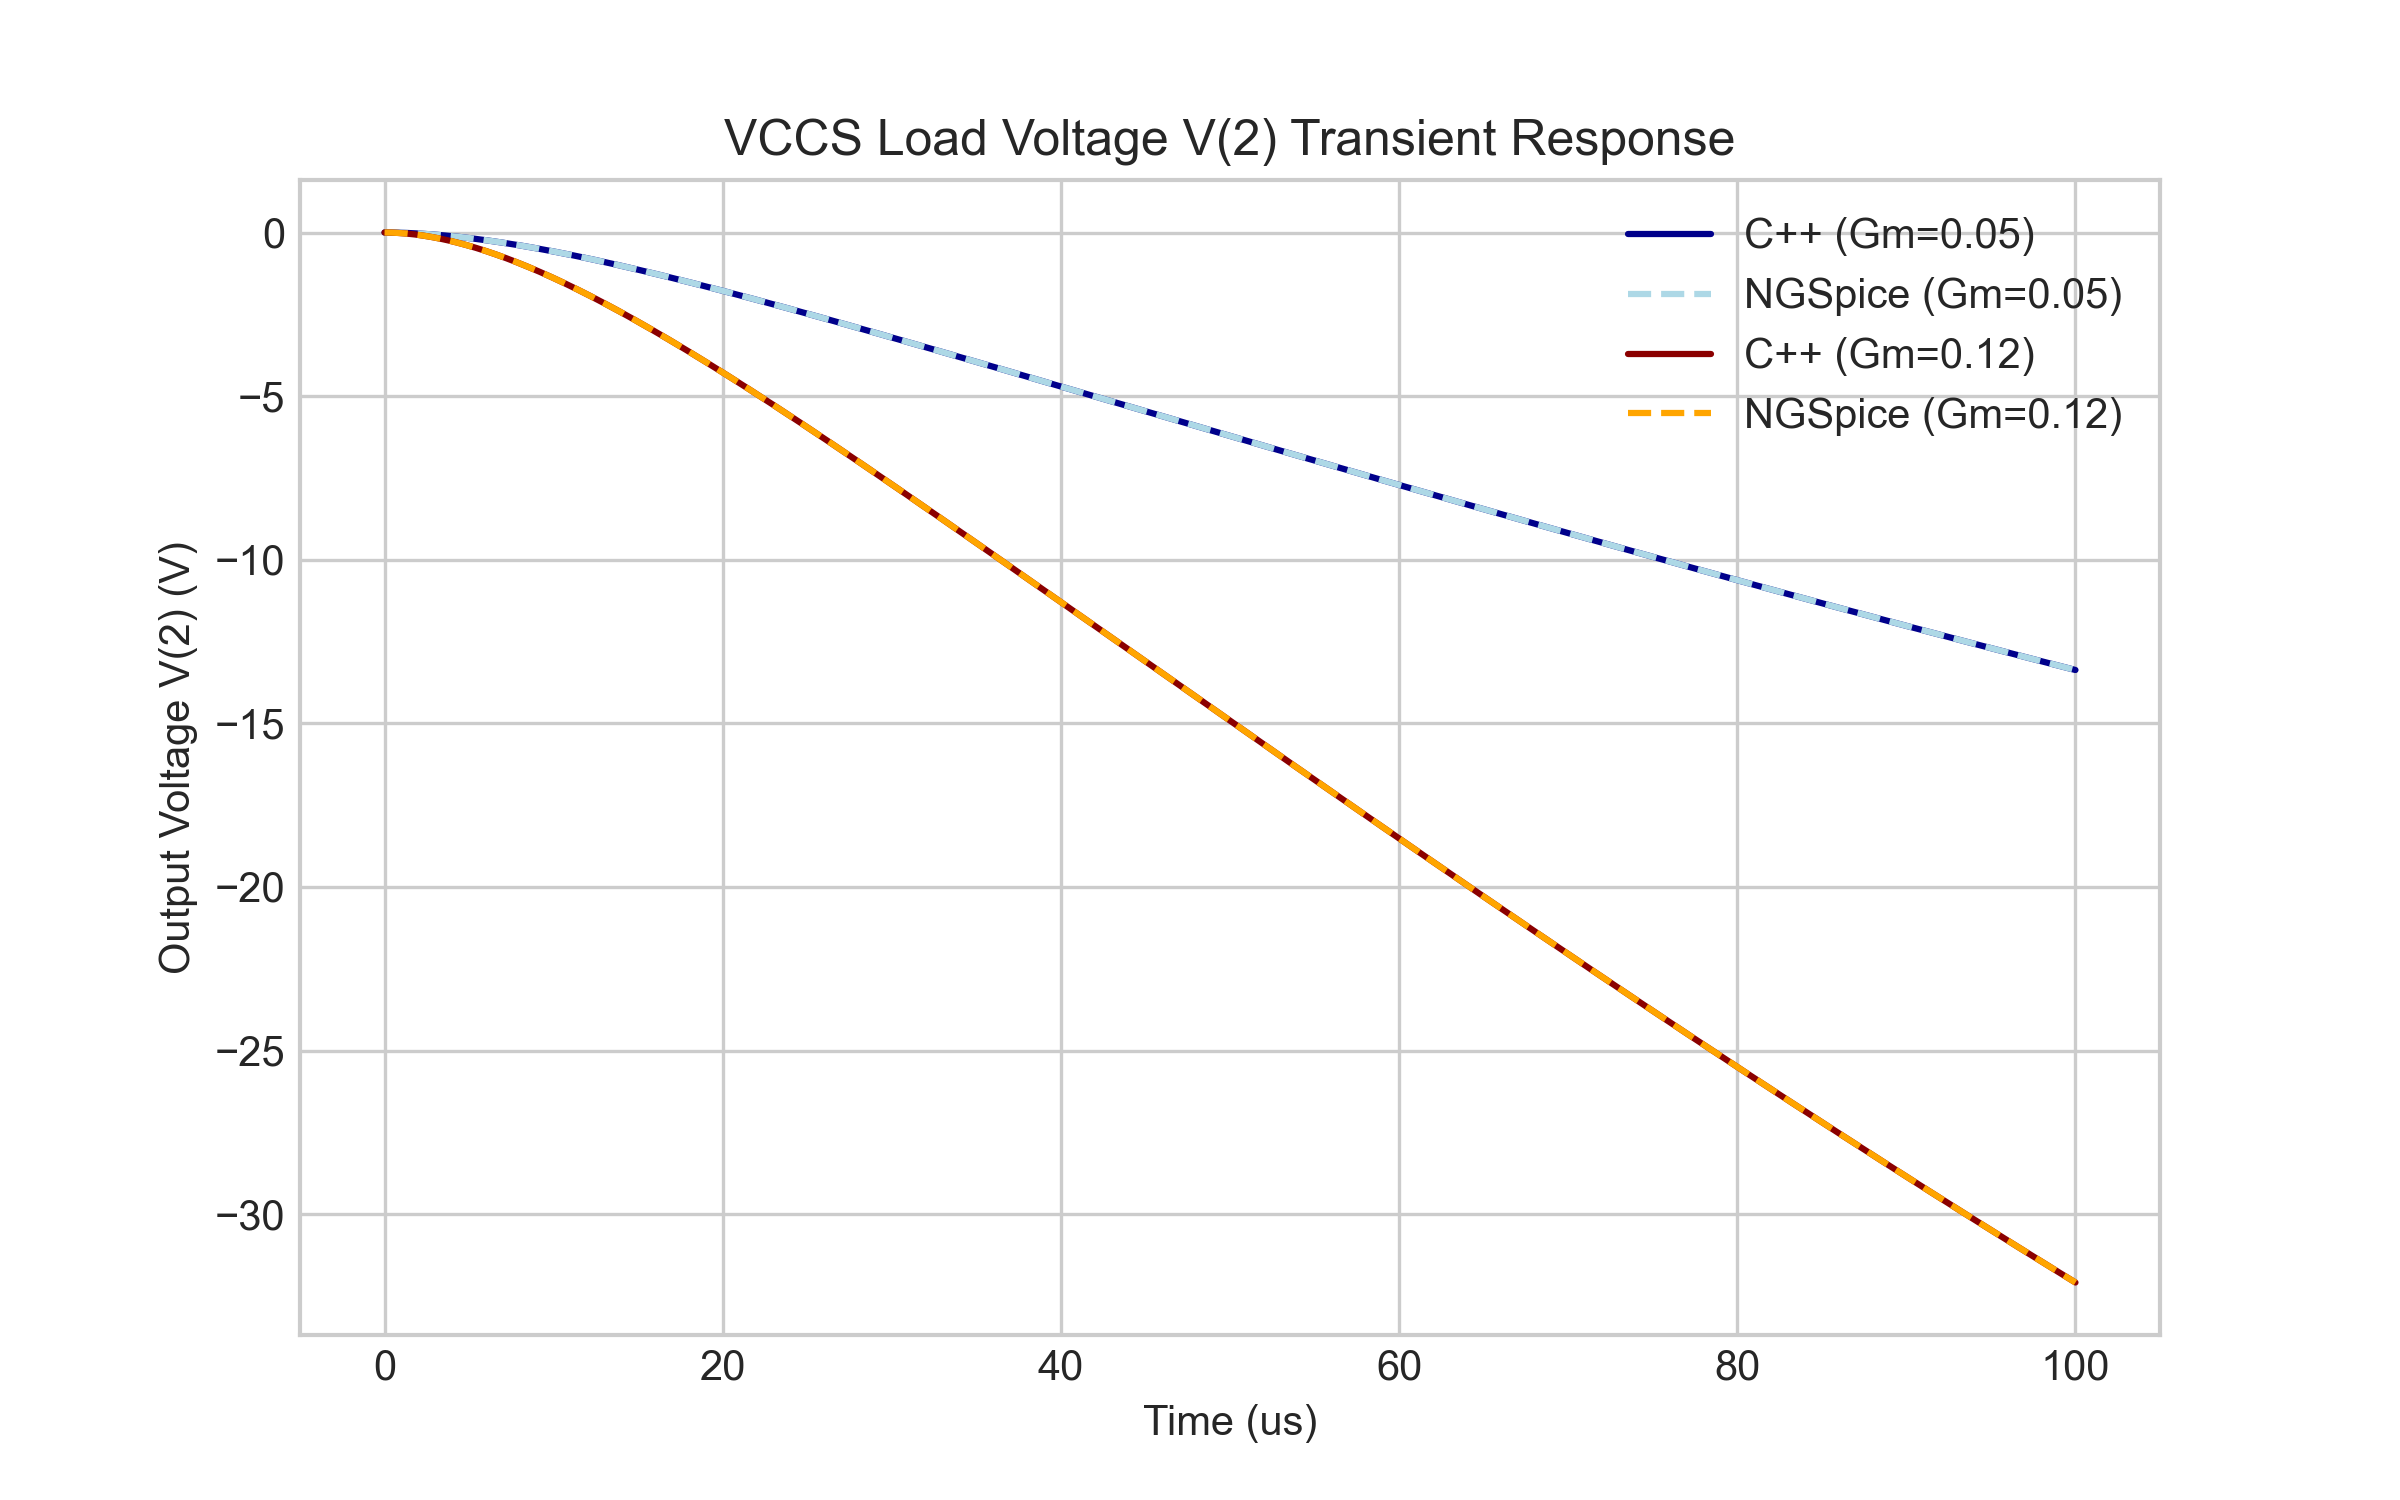
\includegraphics[width=0.6\textwidth]{Figures/Ch5/vccs_3.png}
    \caption{VCCS Transfer Characteristic Test 3.}
    \label{fig:vccs_test_3}
\end{figure}

\subsection{Voltage-Controlled Voltage Source (VCVS)}
The VCVS unit tests verify voltage transfer function accuracy and auxiliary branch variables.

\subsubsection{Internal C++ Unit Tests}
The C++ testing framework validates the VCVS through an integrated matrix solver sweep:
\begin{itemize}
    \item \textbf{Voltage Transfer Equation:} Confirms that the output voltage tracks the linear voltage gain ($E$) times the controlling voltage drop, ensuring correct behavior of the dual-node interaction.
    \item \textbf{Branch Row Stamping:} Verifies that the required auxiliary branch current variable is properly integrated into the MNA matrix, with $+1$ and $-1$ voltage constraint stamps.
    \item \textbf{Linear Sweep Simulation:} Validates the VCVS algebraic boundary constraints during a DC input voltage sweep by solving the fully-coupled conductance matrix via Gaussian elimination.
\end{itemize}

\subsubsection{NGSpice Verification}
Figures~\ref{fig:vcvs_test_1} to \ref{fig:vcvs_test_3} illustrate the NGSpice verification plots for the VCVS. The solved auxiliary branch currents and nodal voltages closely match the baseline NGSpice references under varying load conditions.

\begin{figure}[H]
    \centering
    \begin{minipage}{0.48\textwidth}
        \centering
        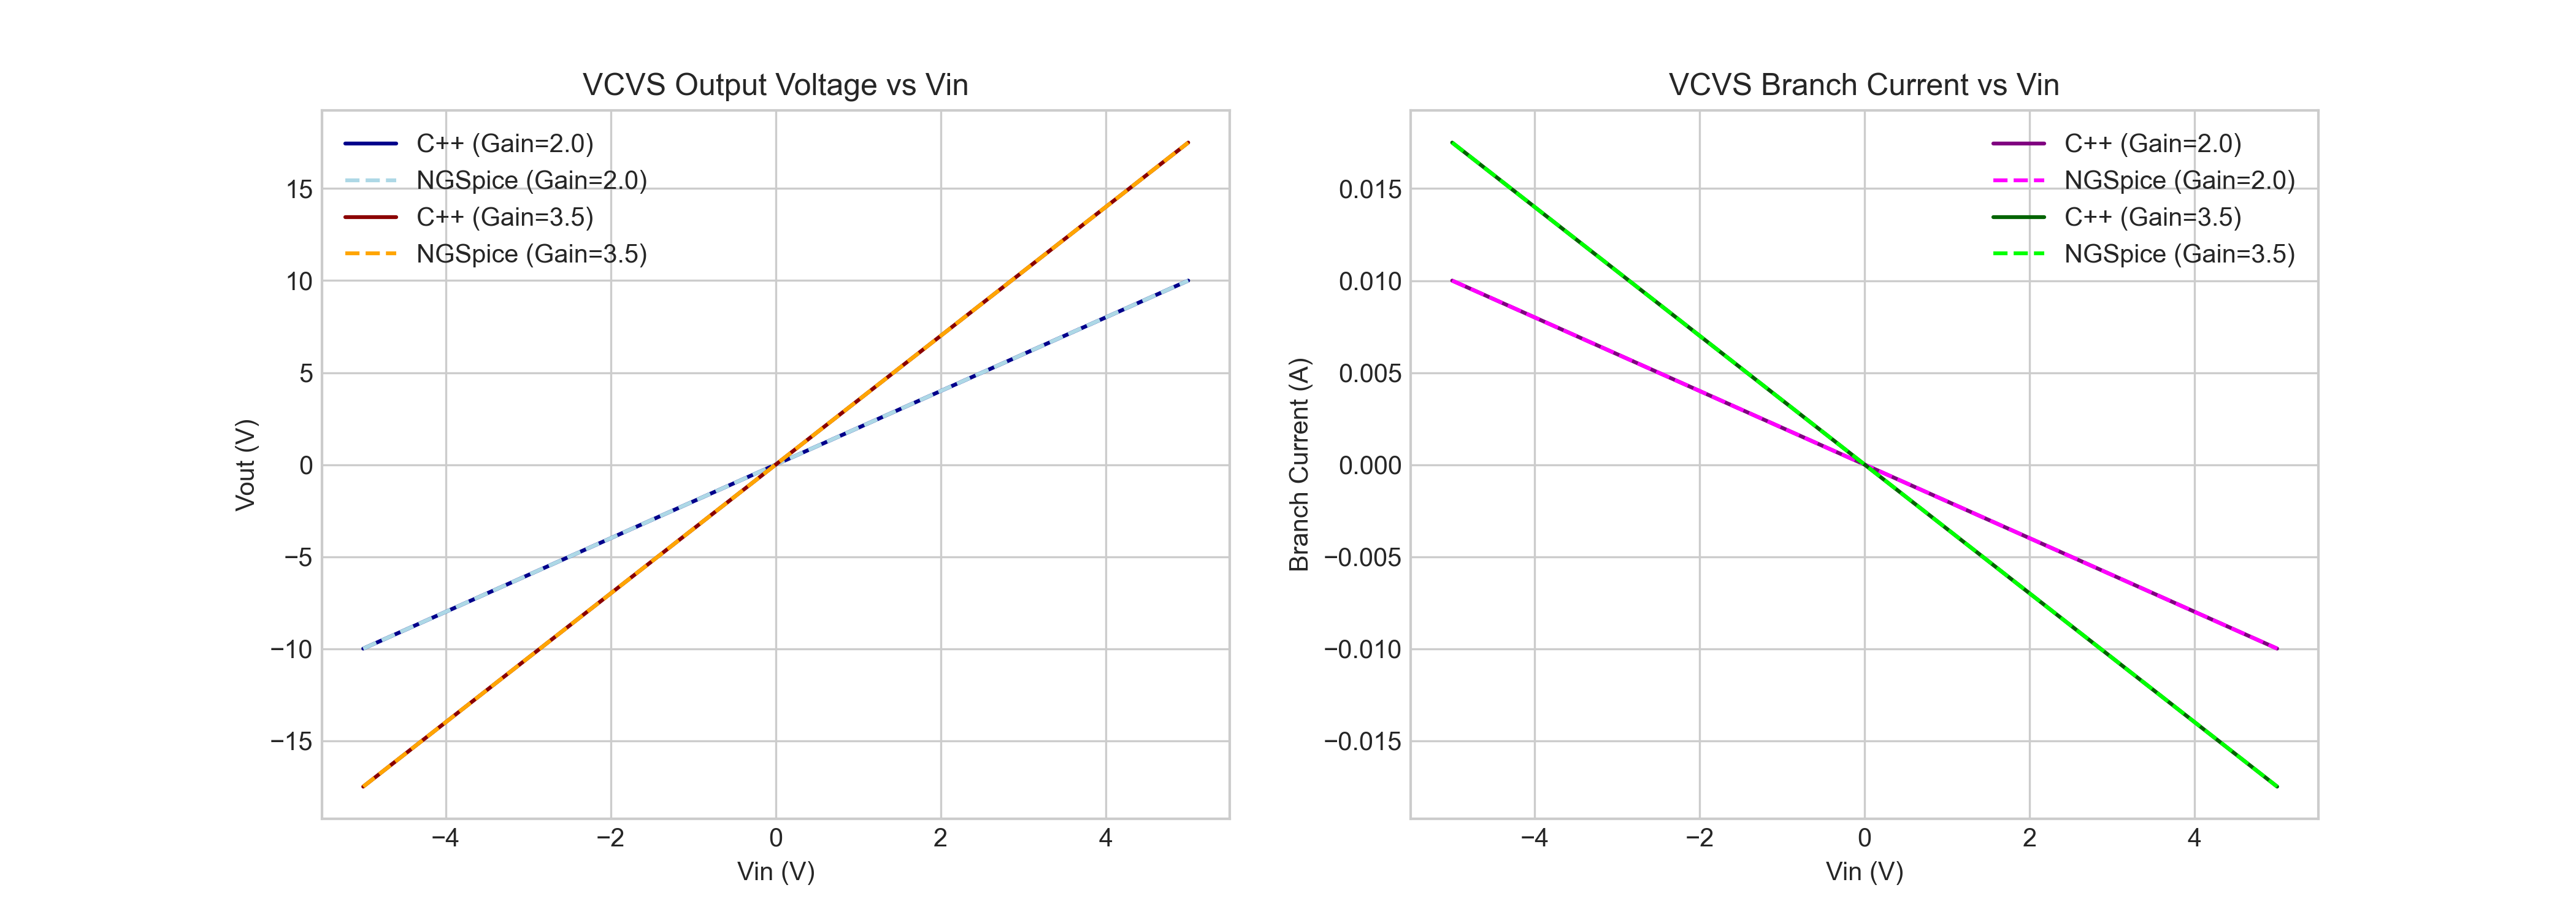
\includegraphics[width=\linewidth]{Figures/Ch5/vcvs_1.png}
        \caption{VCVS Voltage Transfer Test 1.}
        \label{fig:vcvs_test_1}
    \end{minipage}\hfill
    \begin{minipage}{0.48\textwidth}
        \centering
        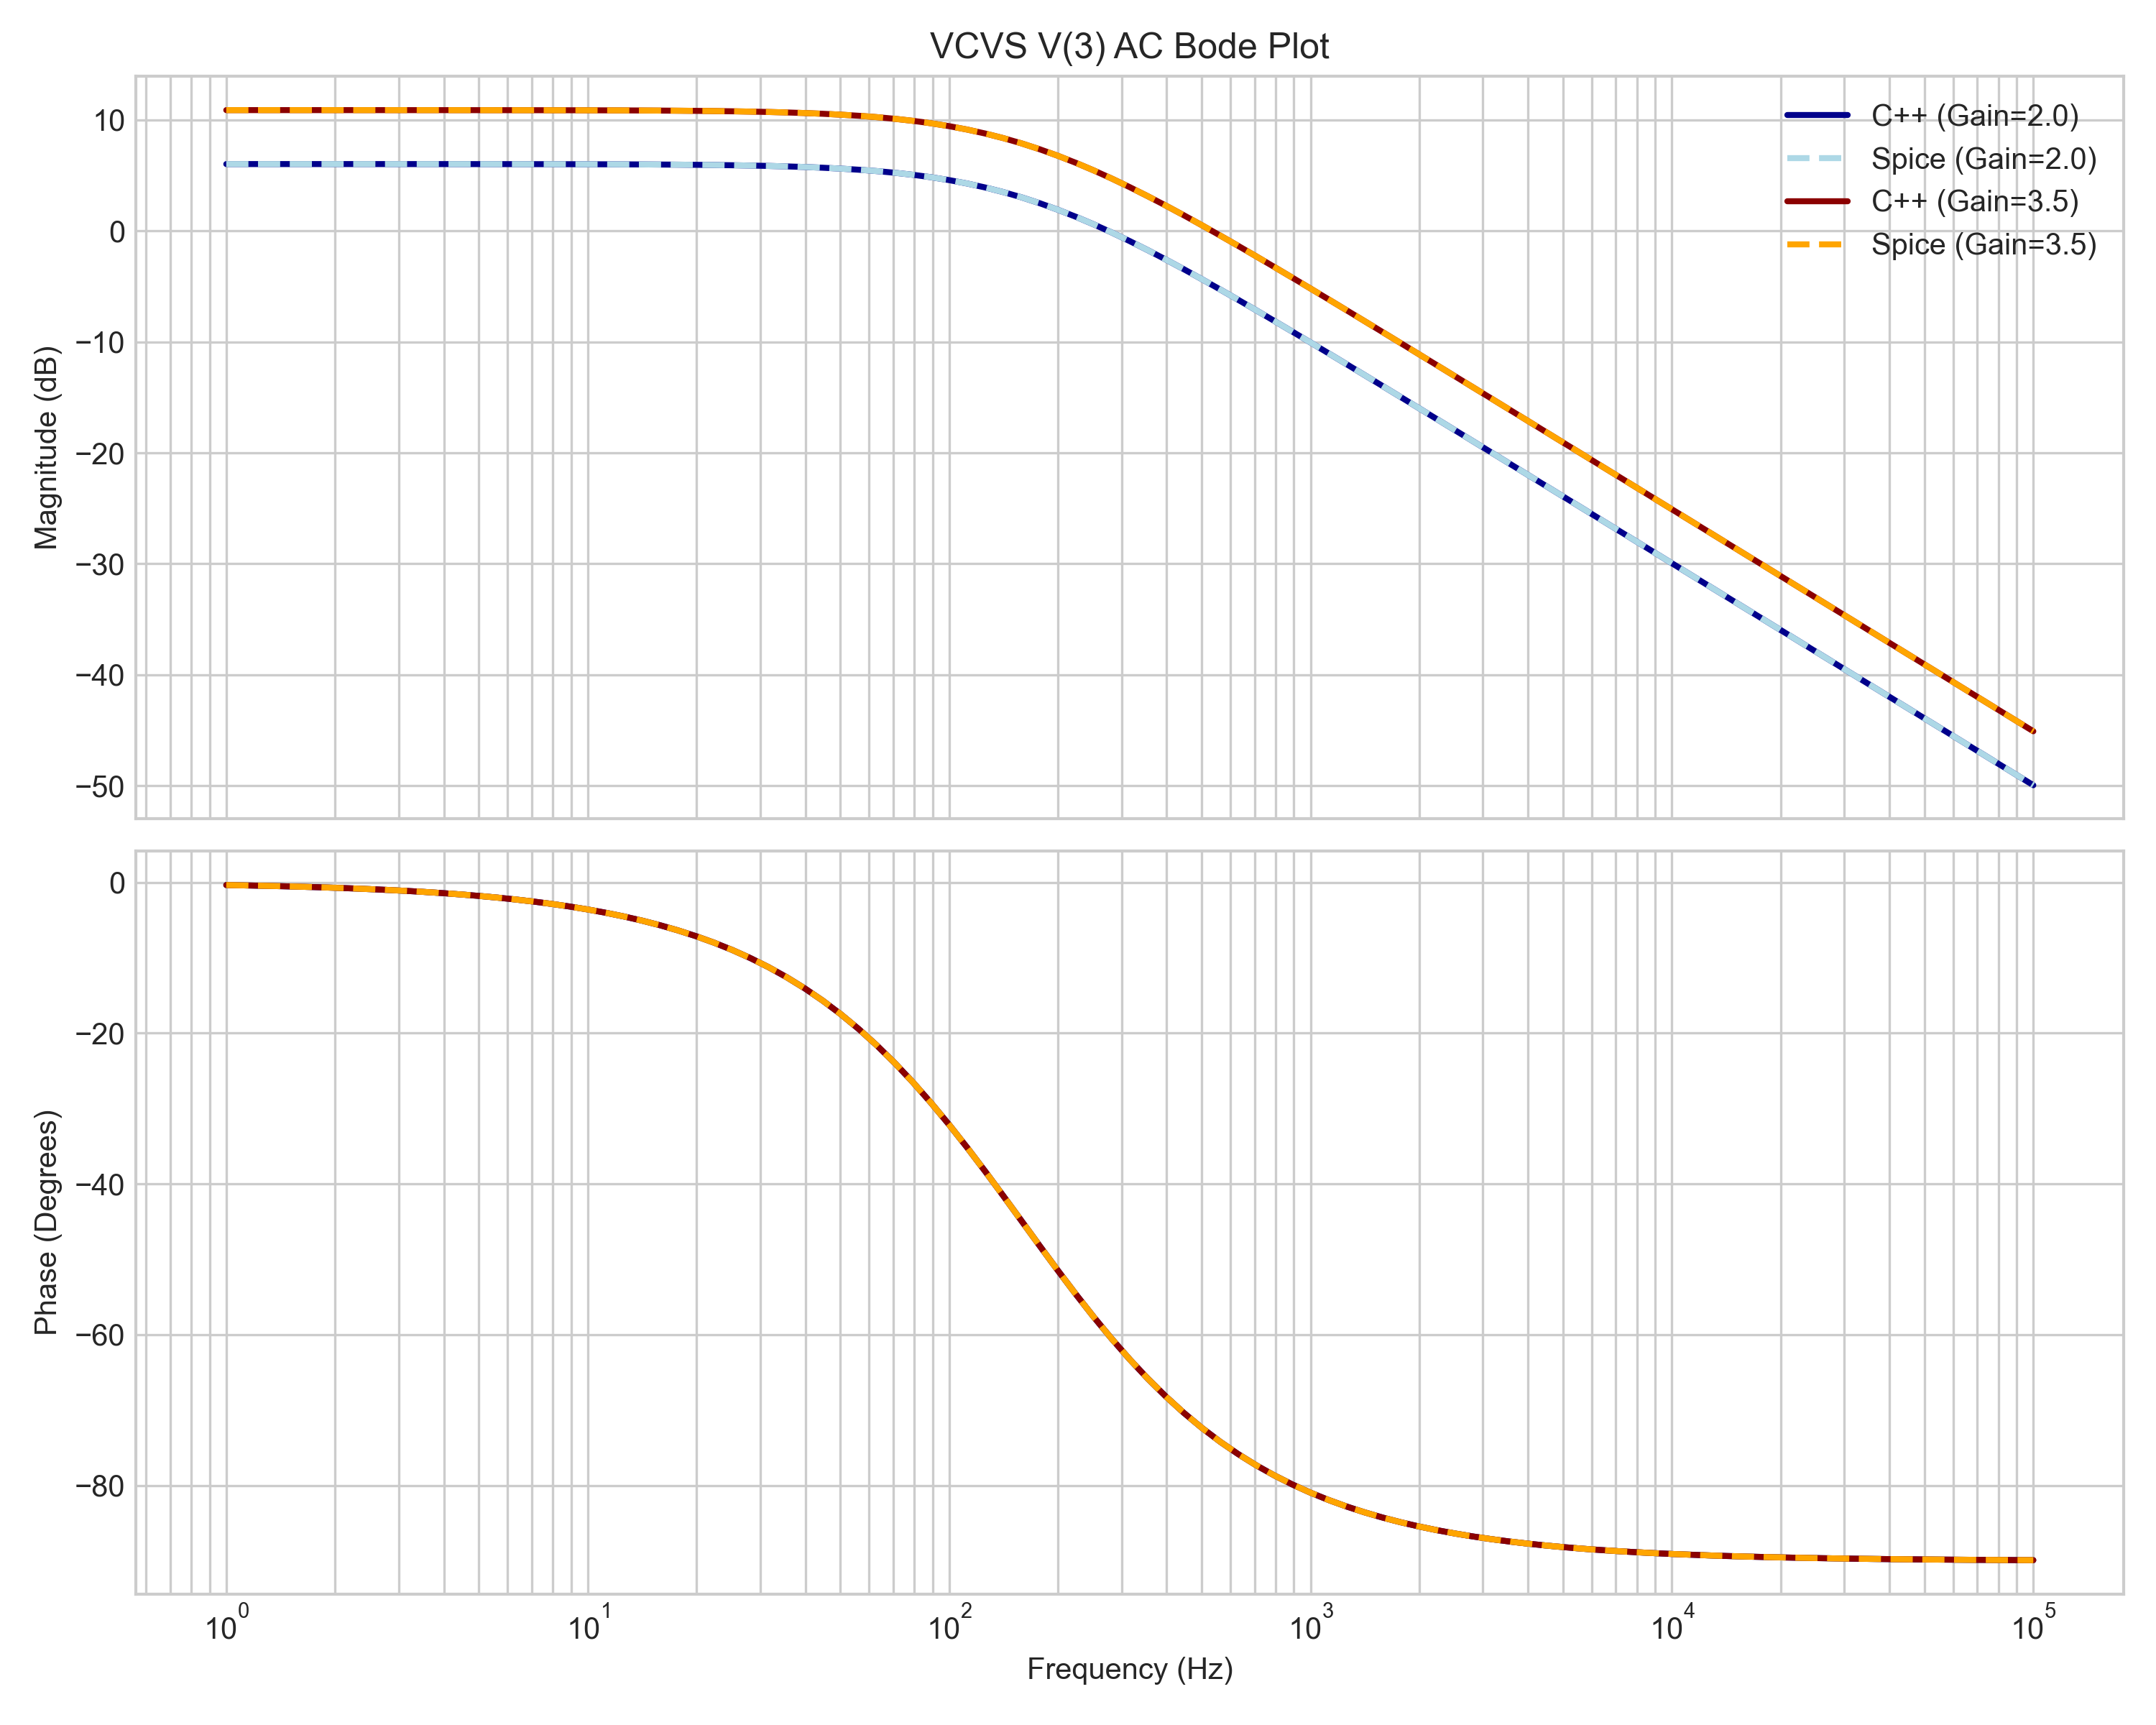
\includegraphics[width=\linewidth]{Figures/Ch5/vcvs_2.png}
        \caption{VCVS Voltage Transfer Test 2.}
        \label{fig:vcvs_test_2}
    \end{minipage}
\end{figure}

\begin{figure}[H]
    \centering
    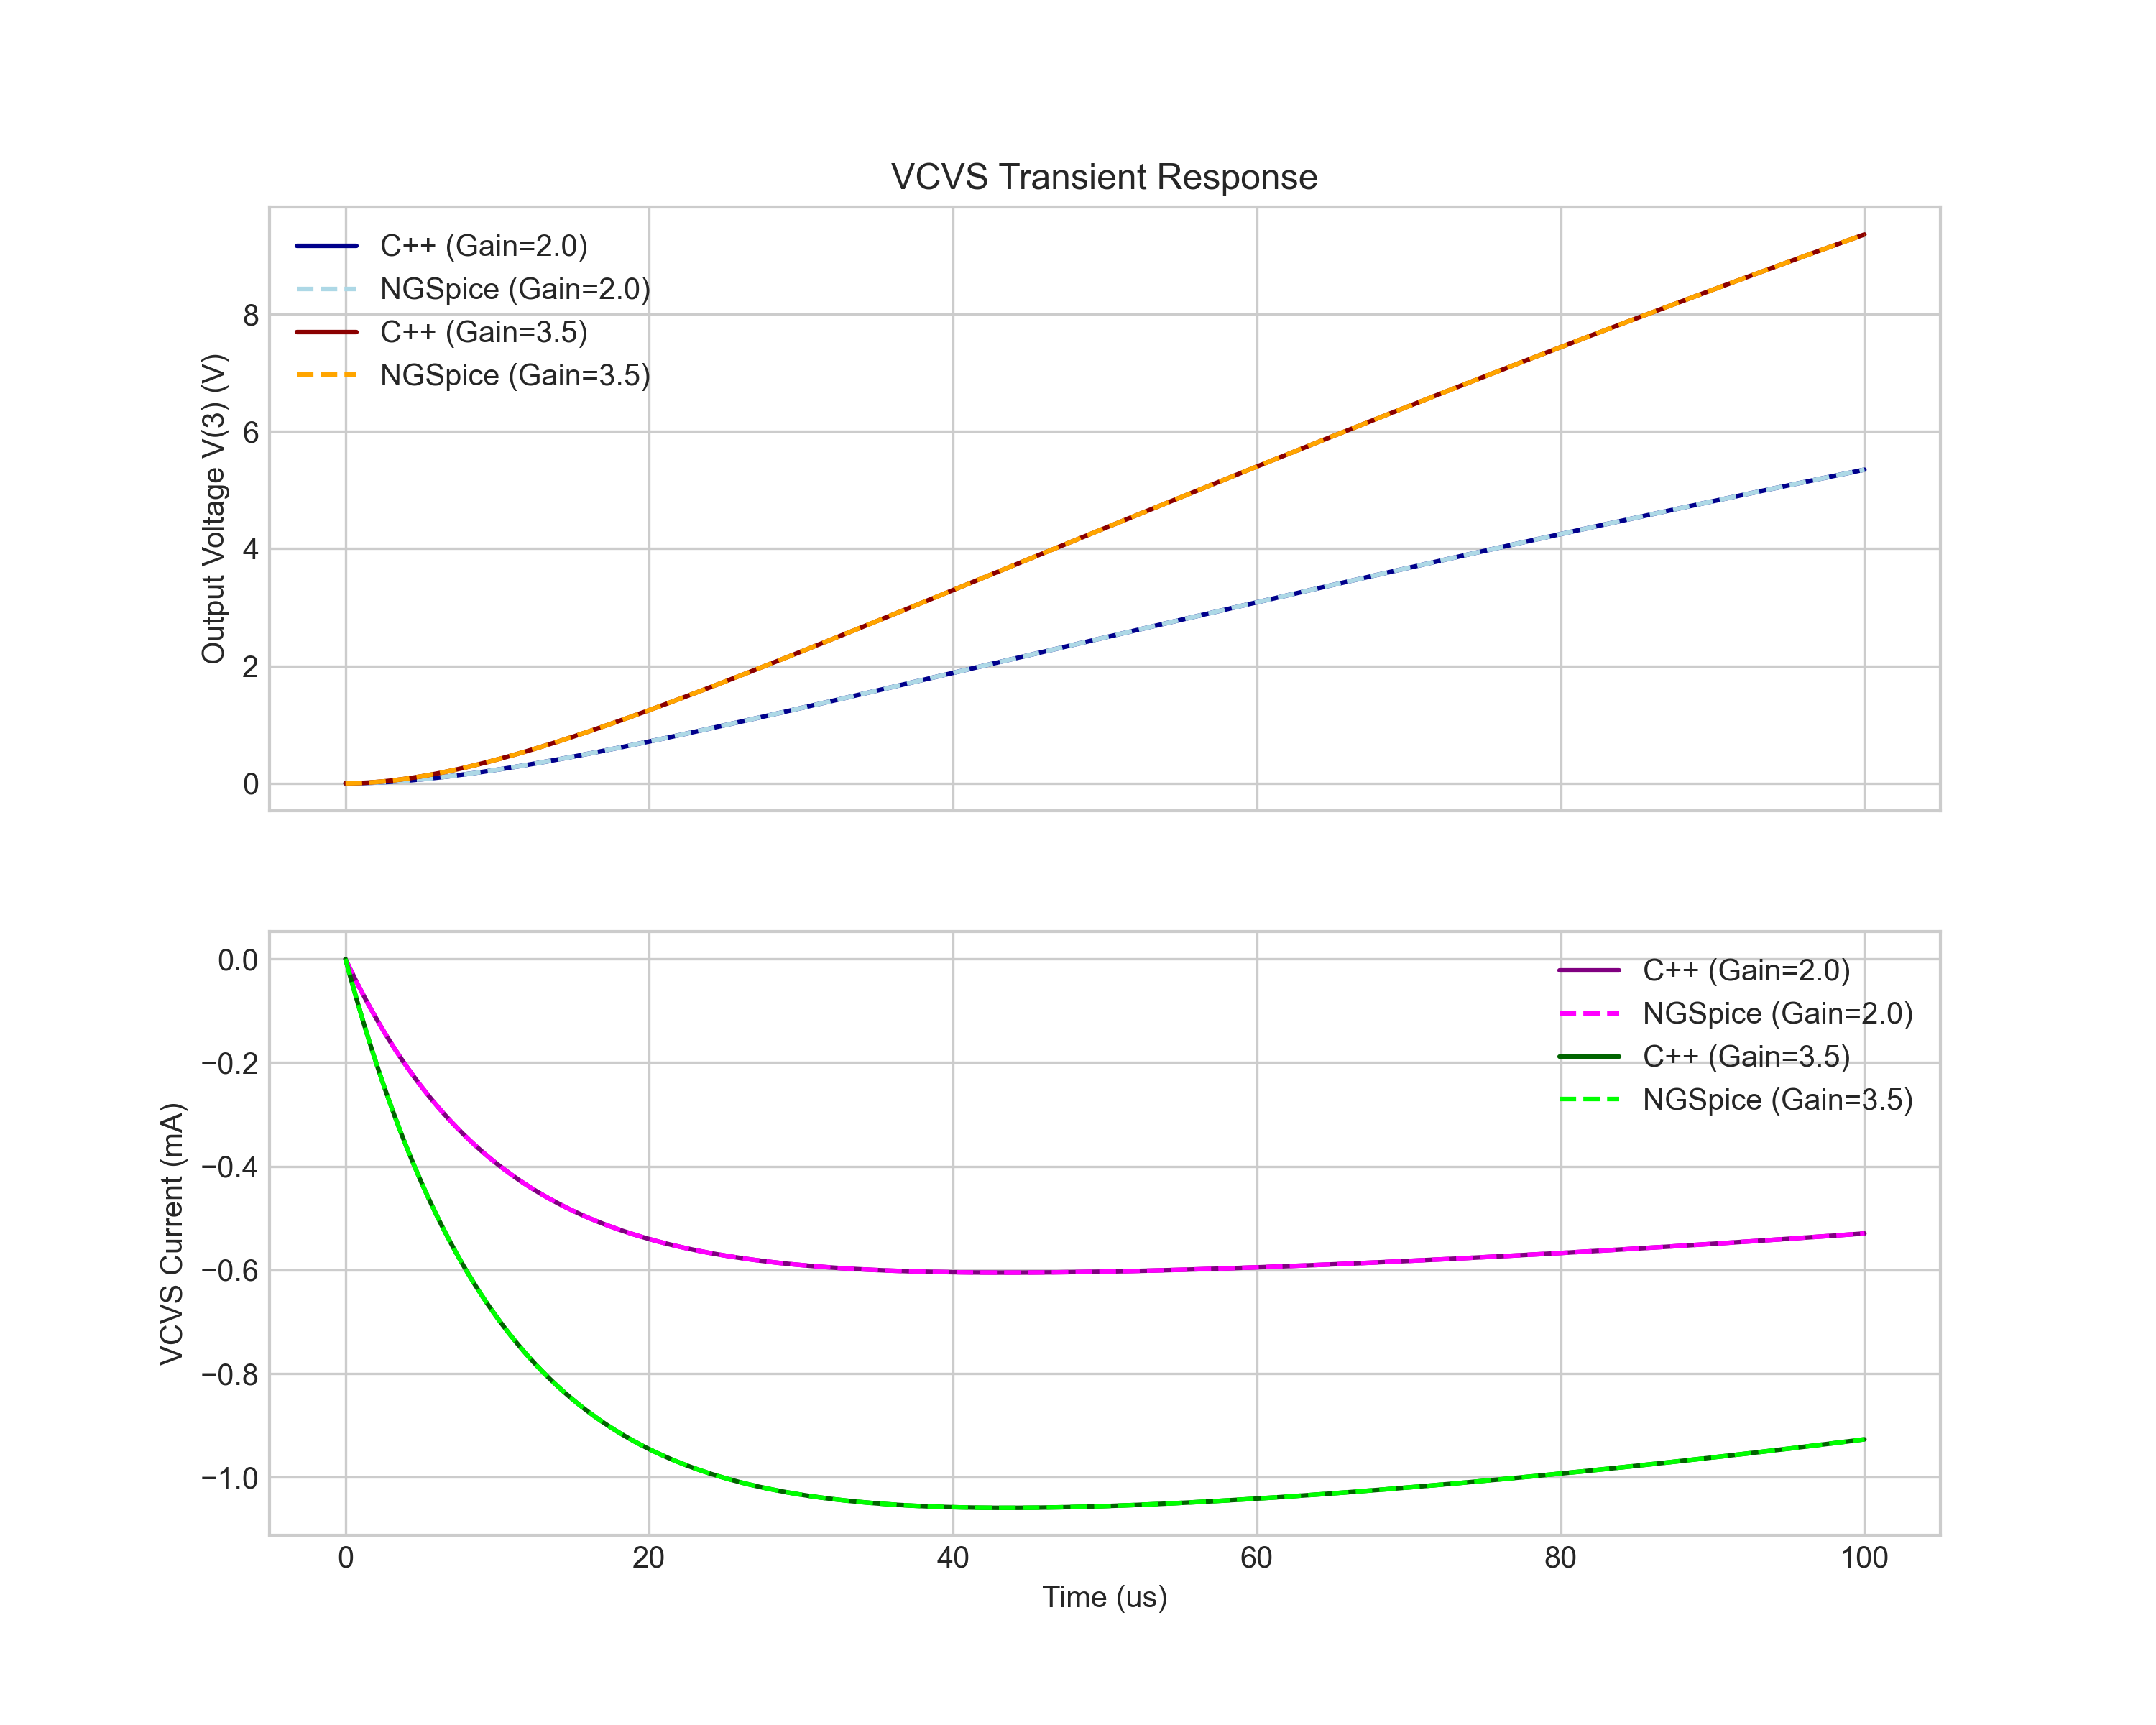
\includegraphics[width=0.6\textwidth]{Figures/Ch5/vcvs_3.png}
    \caption{VCVS Voltage Transfer Test 3.}
    \label{fig:vcvs_test_3}
\end{figure}

\subsection{Current-Controlled Current Source (CCCS)}
The CCCS tests verify output current tracking and sensor branch ammeter functionality.

\subsubsection{Internal C++ Unit Tests}
The C++ testing framework validates the CCCS through an integrated matrix solver sweep:
\begin{itemize}
    \item \textbf{Current Control Mechanism:} Validates that the output current strictly tracks the linear current gain ($F$) multiplied by the current flowing through a specified sensing branch.
    \item \textbf{Sensing Branch Integration:} Verifies the complex dependency of the MNA matrix on the current state of an external branch index, ensuring correct tracking of branch indices.
    \item \textbf{Linear Sweep Simulation:} Confirms KCL and matrix stability during a full sweep of the source excitation while tracking the sensor branch variations via Gaussian elimination.
\end{itemize}

\subsubsection{NGSpice Verification}
Figures~\ref{fig:cccs_test_1} to \ref{fig:cccs_test_6} illustrate the NGSpice verification plots for the CCCS. The figures confirm the successful linear tracking of branch currents and validate the numeric outputs generated by the C++ test harness.

\begin{figure}[H]
    \centering
    \begin{minipage}{0.48\textwidth}
        \centering
        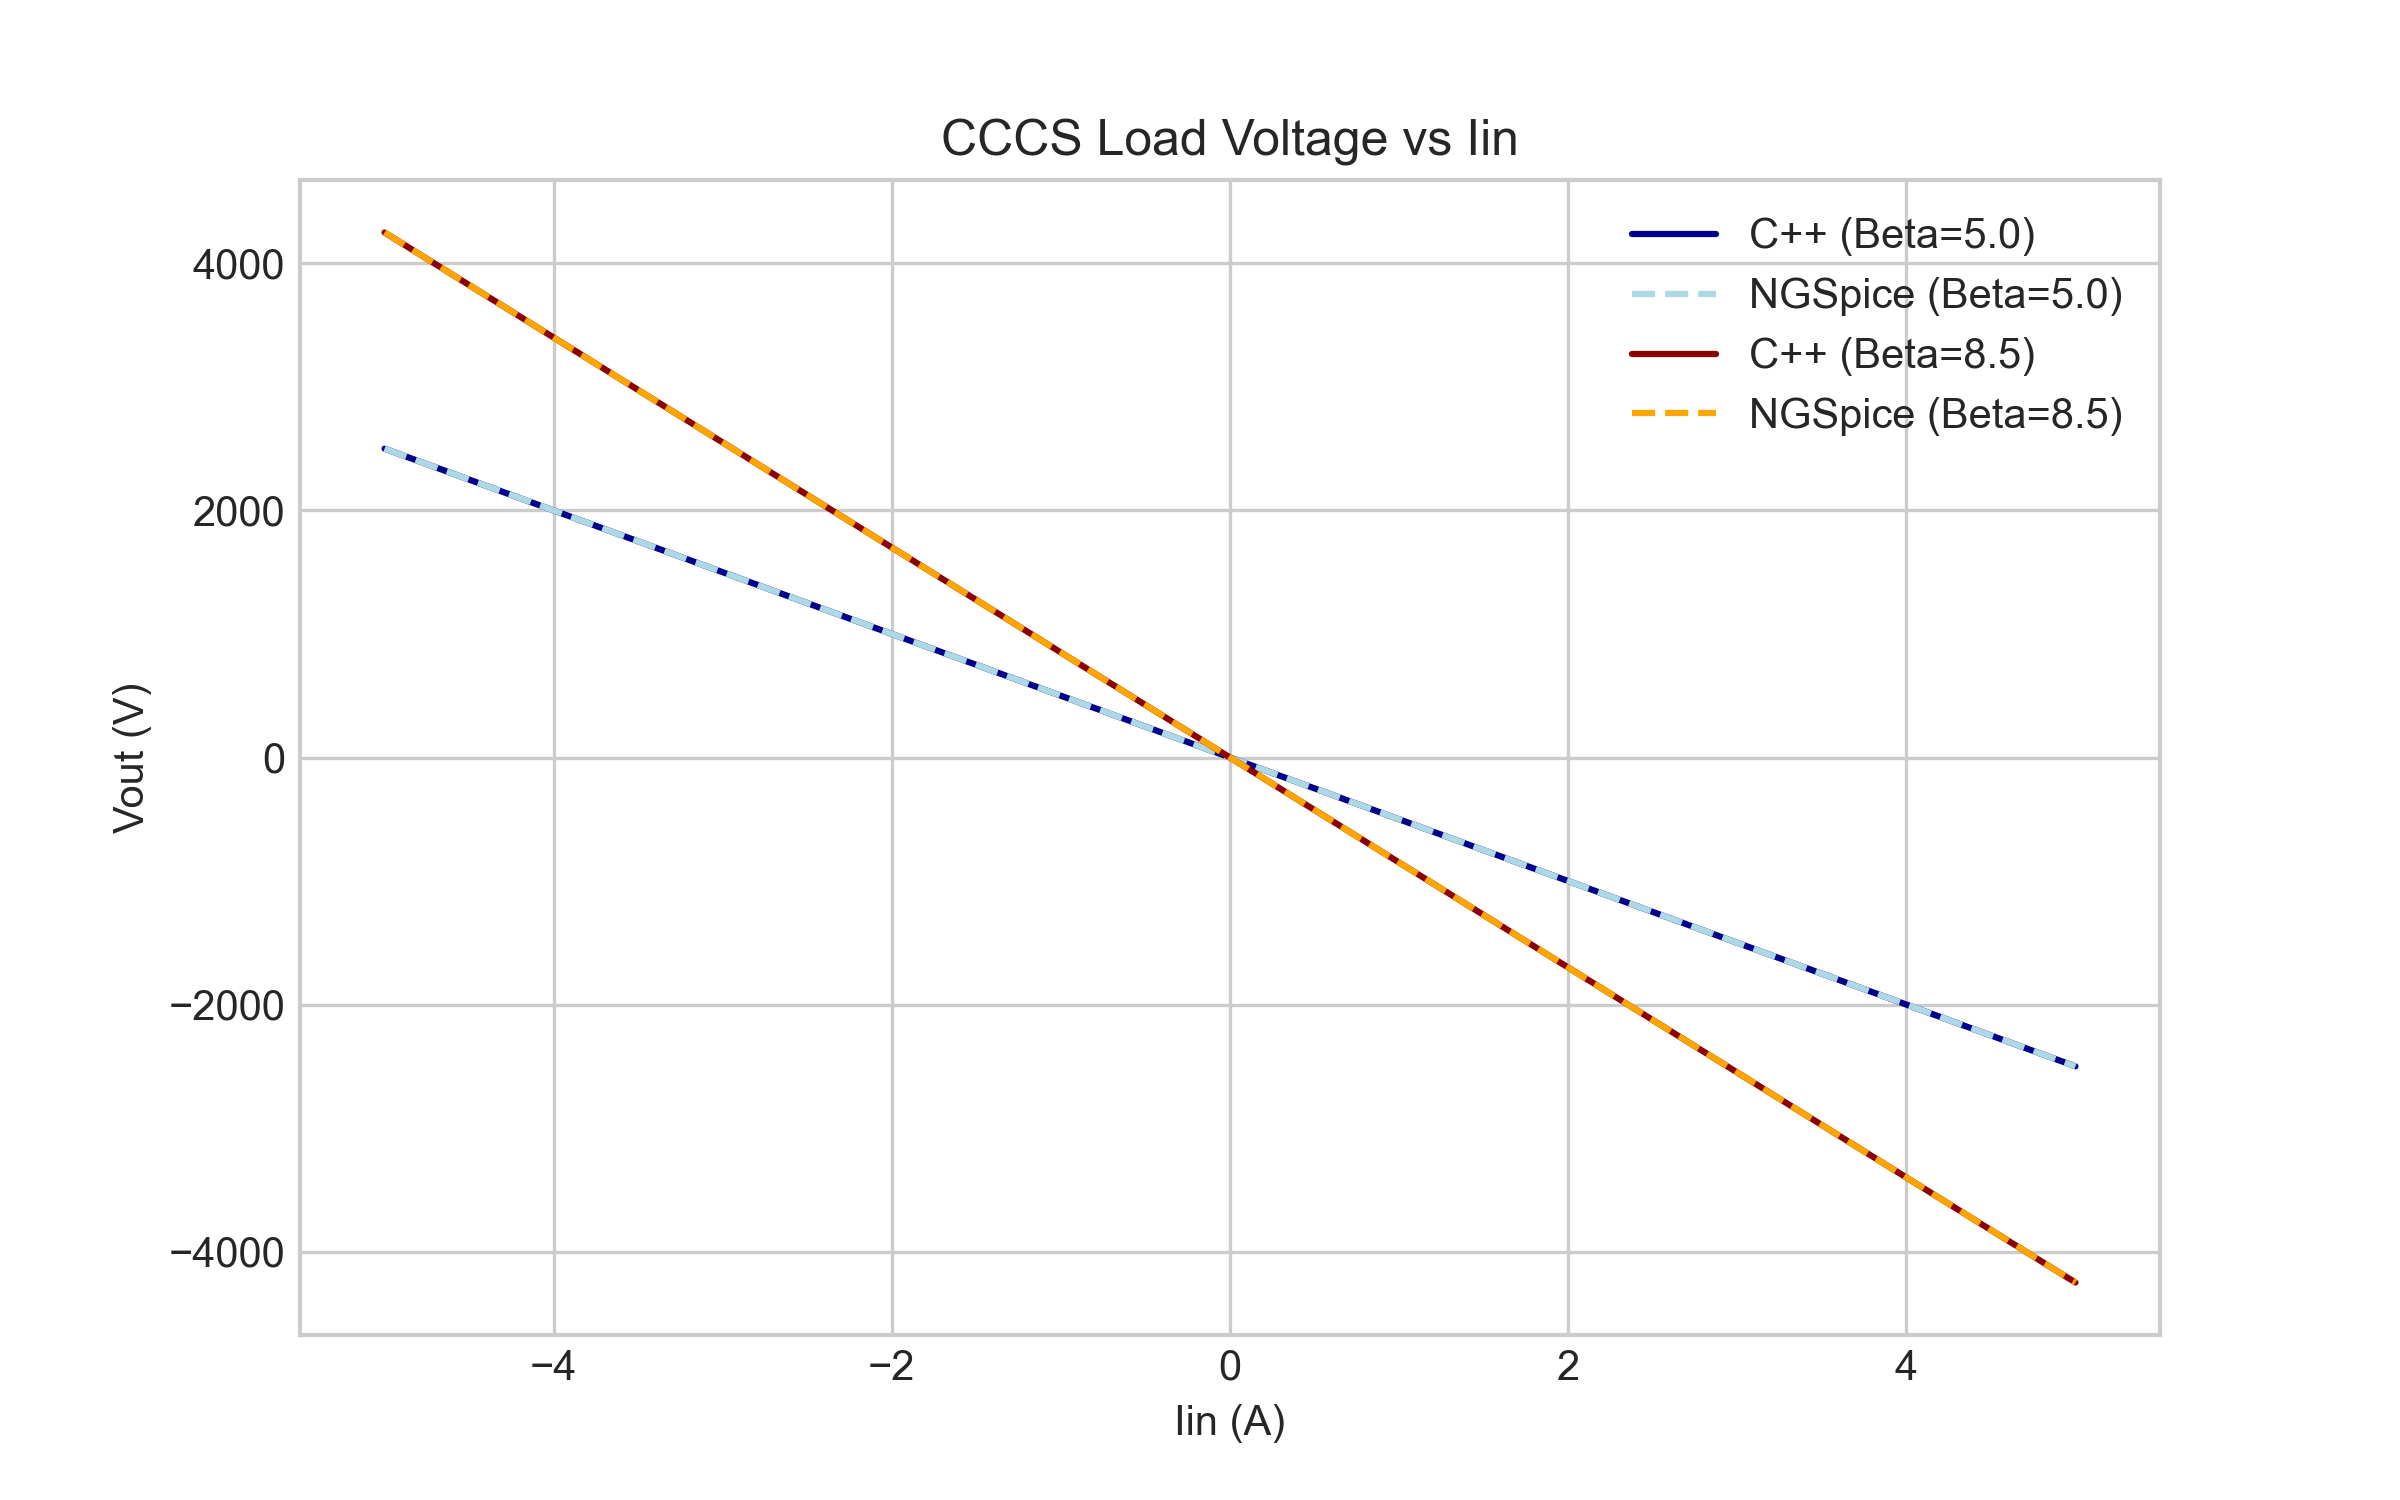
\includegraphics[width=\linewidth]{Figures/Ch5/cccs_1.png}
        \caption{CCCS Current Transfer Test 1.}
        \label{fig:cccs_test_1}
    \end{minipage}\hfill
    \begin{minipage}{0.48\textwidth}
        \centering
        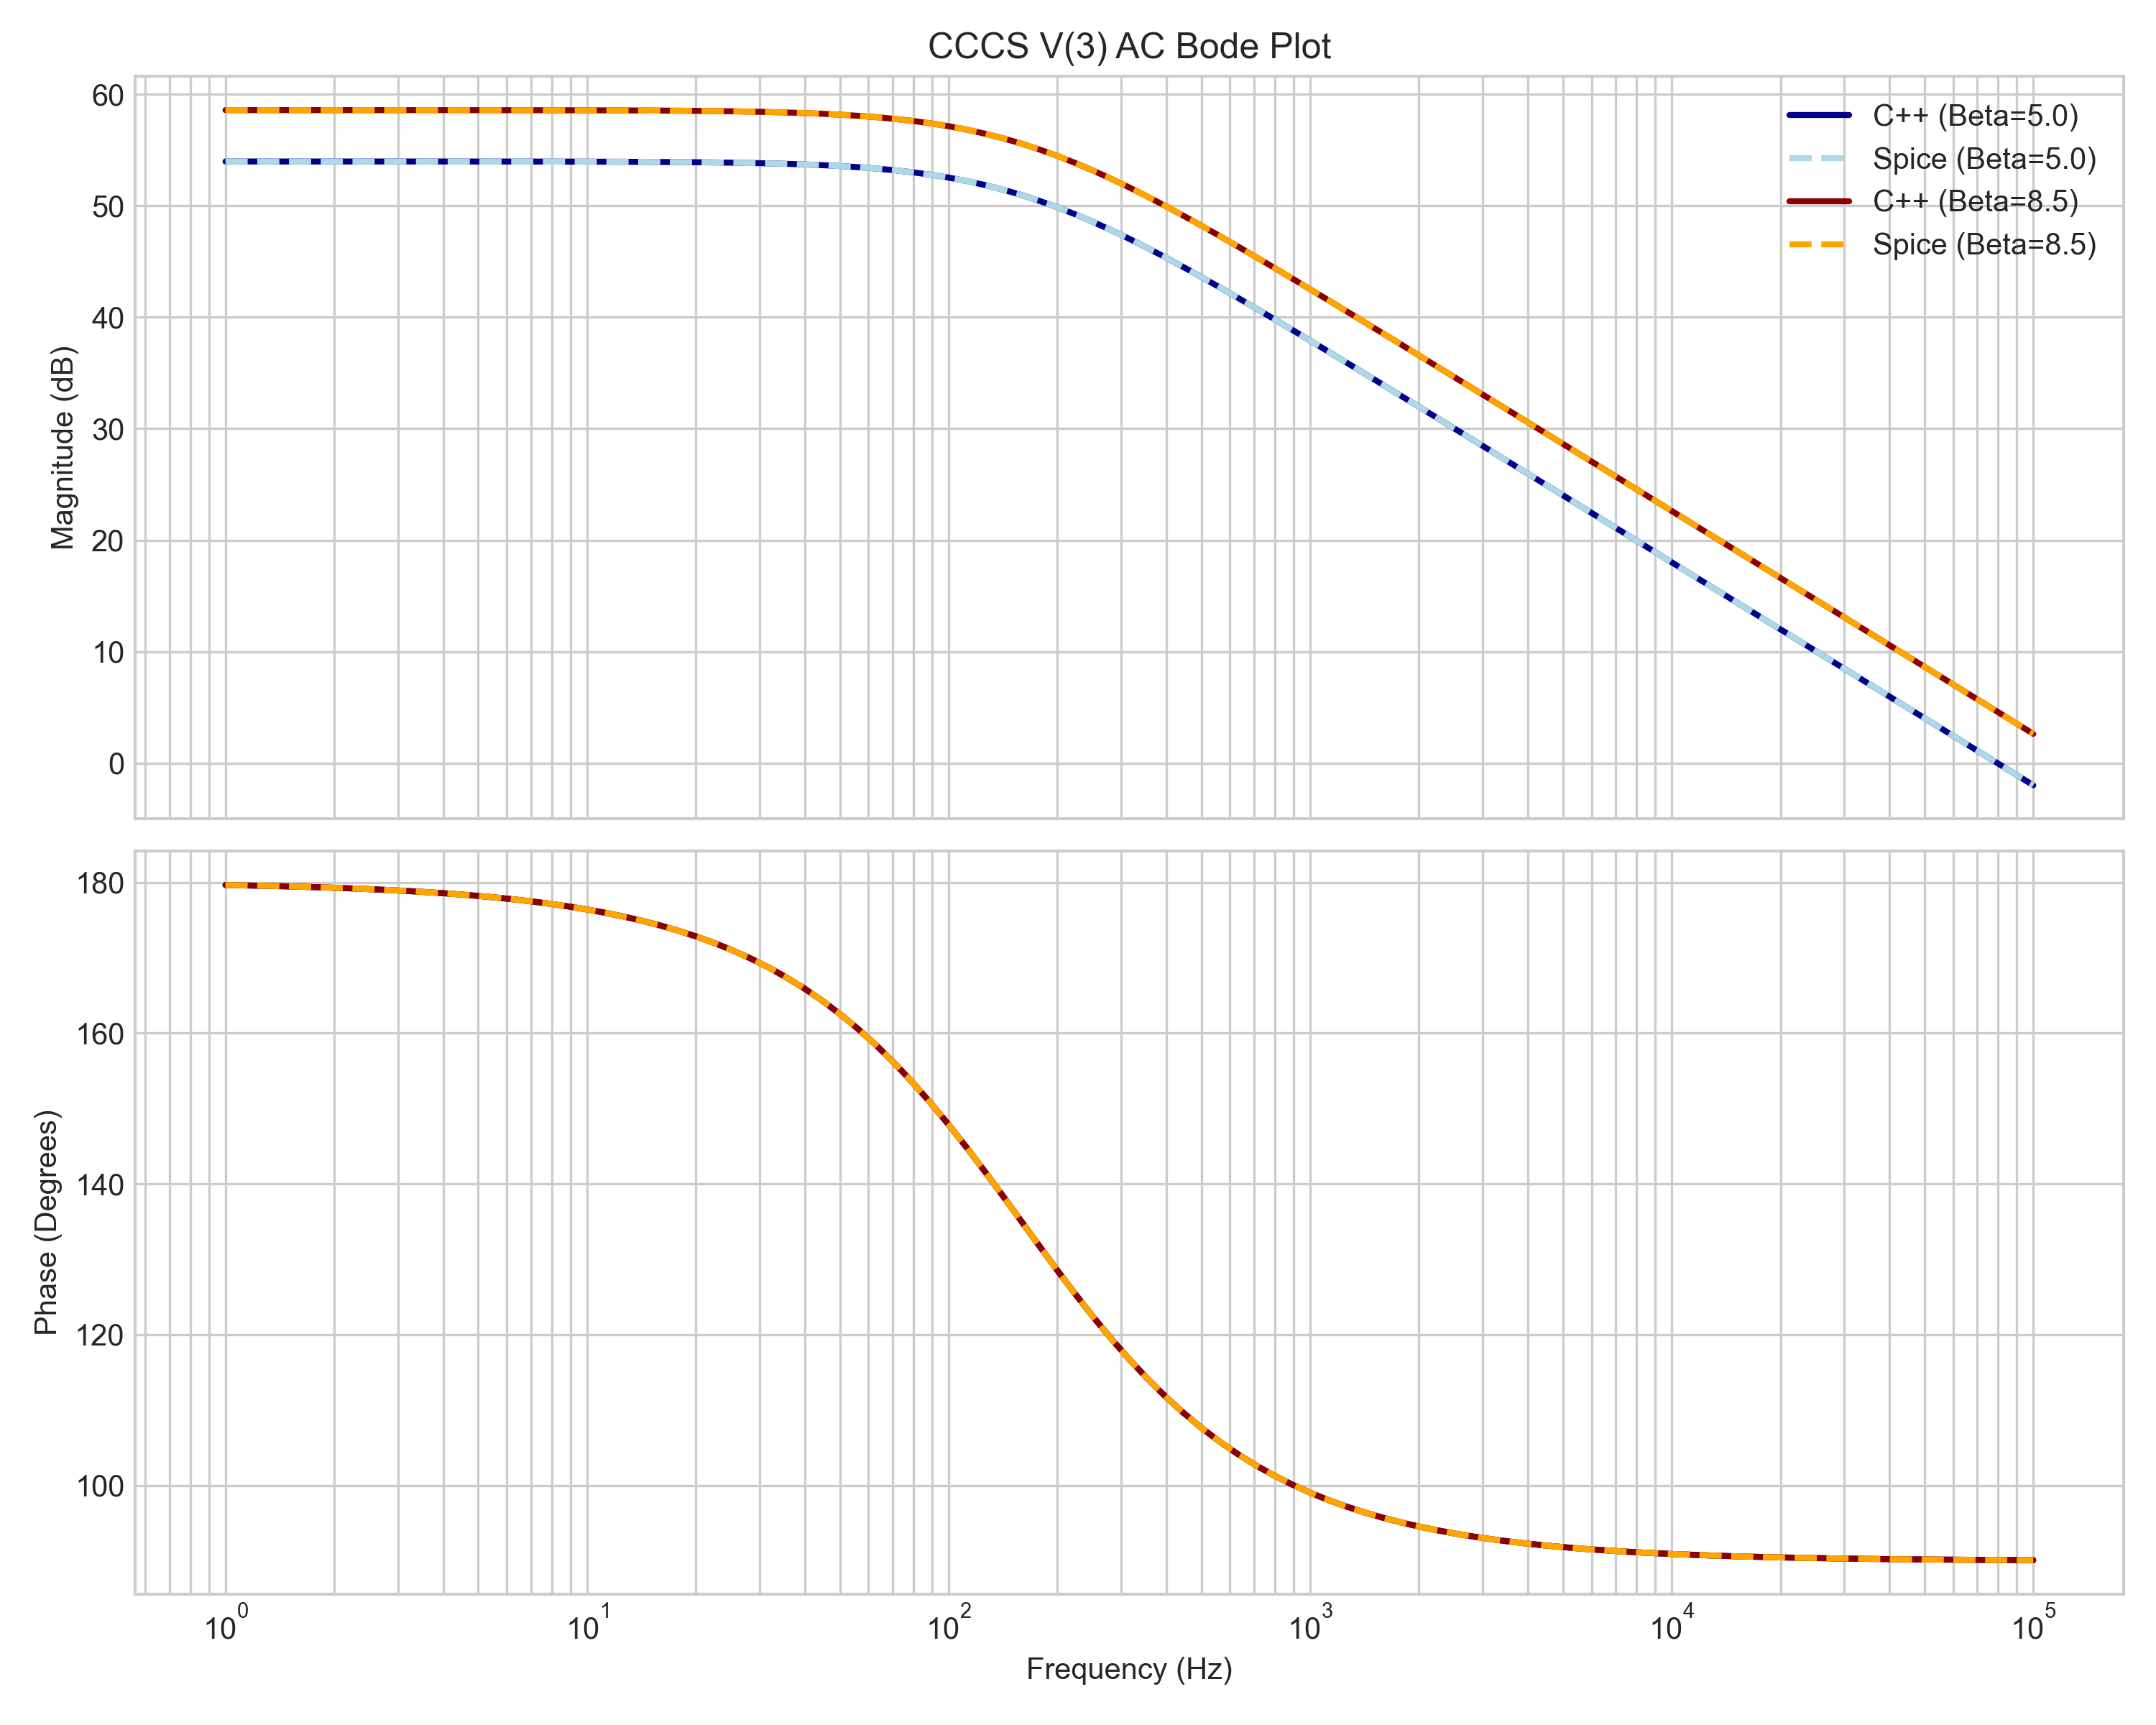
\includegraphics[width=\linewidth]{Figures/Ch5/cccs_2.png}
        \caption{CCCS Current Transfer Test 2.}
        \label{fig:cccs_test_2}
    \end{minipage}
\end{figure}

\begin{figure}[H]
    \centering
    \begin{minipage}{0.48\textwidth}
        \centering
        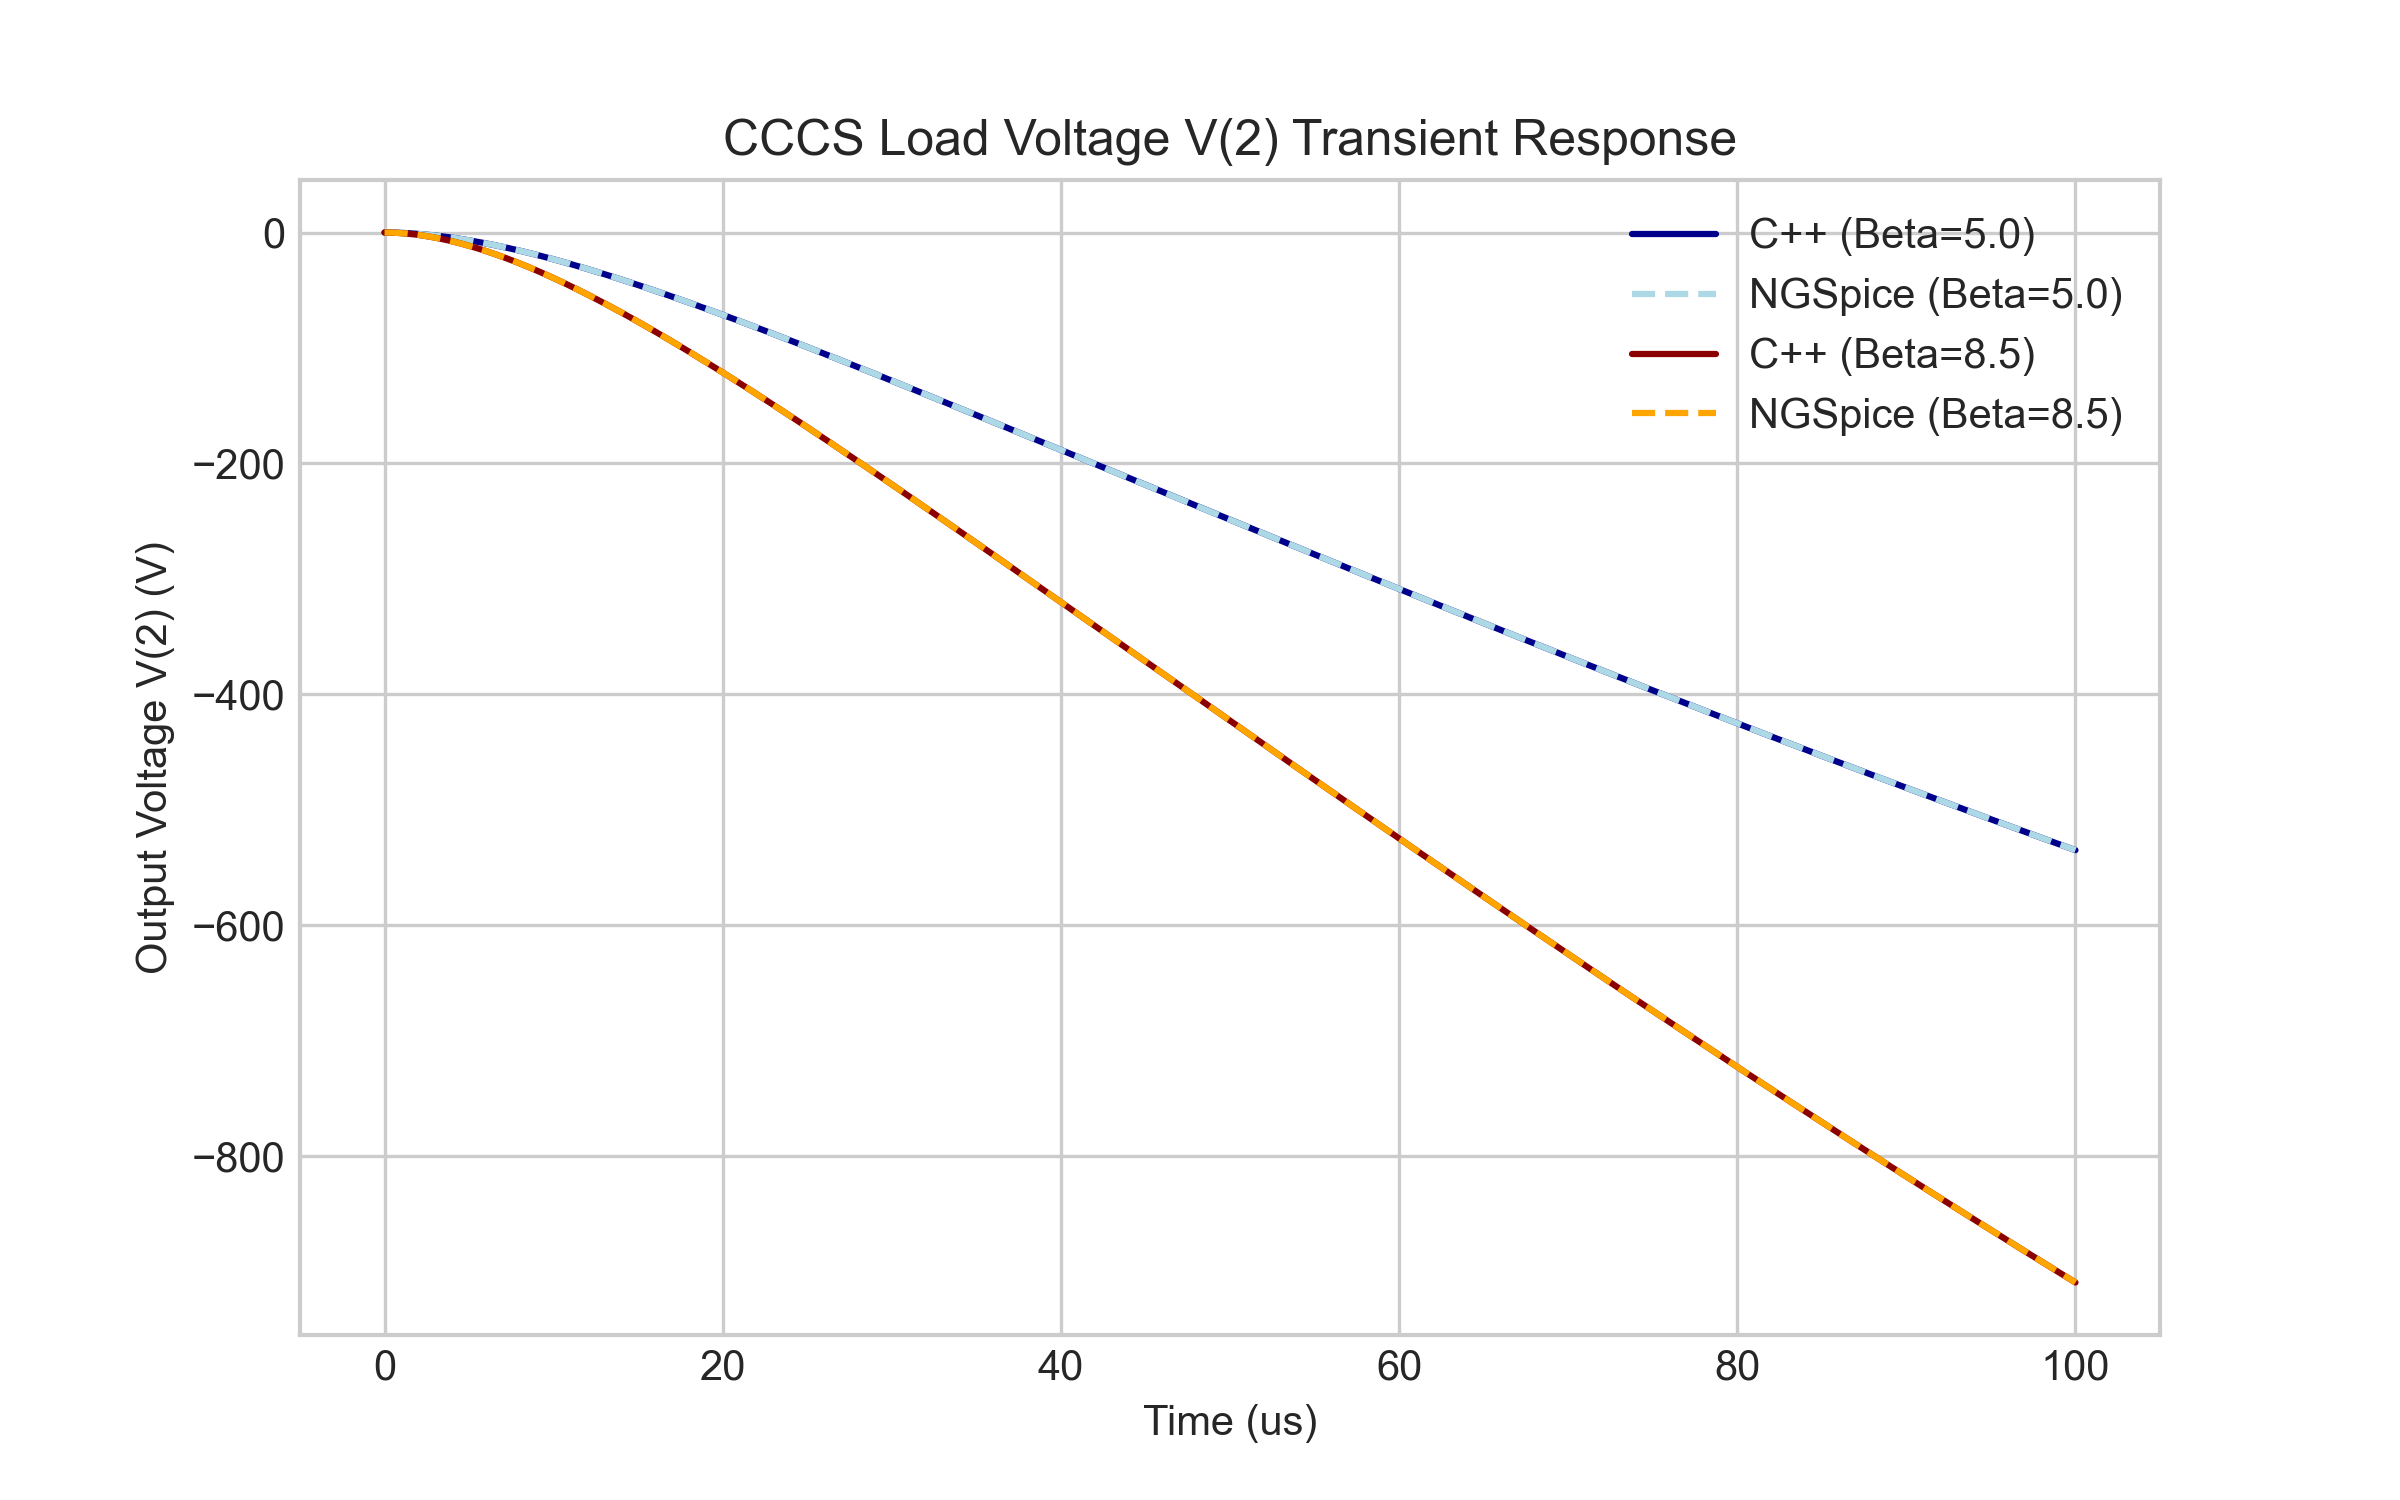
\includegraphics[width=\linewidth]{Figures/Ch5/cccs_3.png}
        \caption{CCCS Current Transfer Test 3.}
        \label{fig:cccs_test_3}
    \end{minipage}\hfill
    \begin{minipage}{0.48\textwidth}
        \centering
        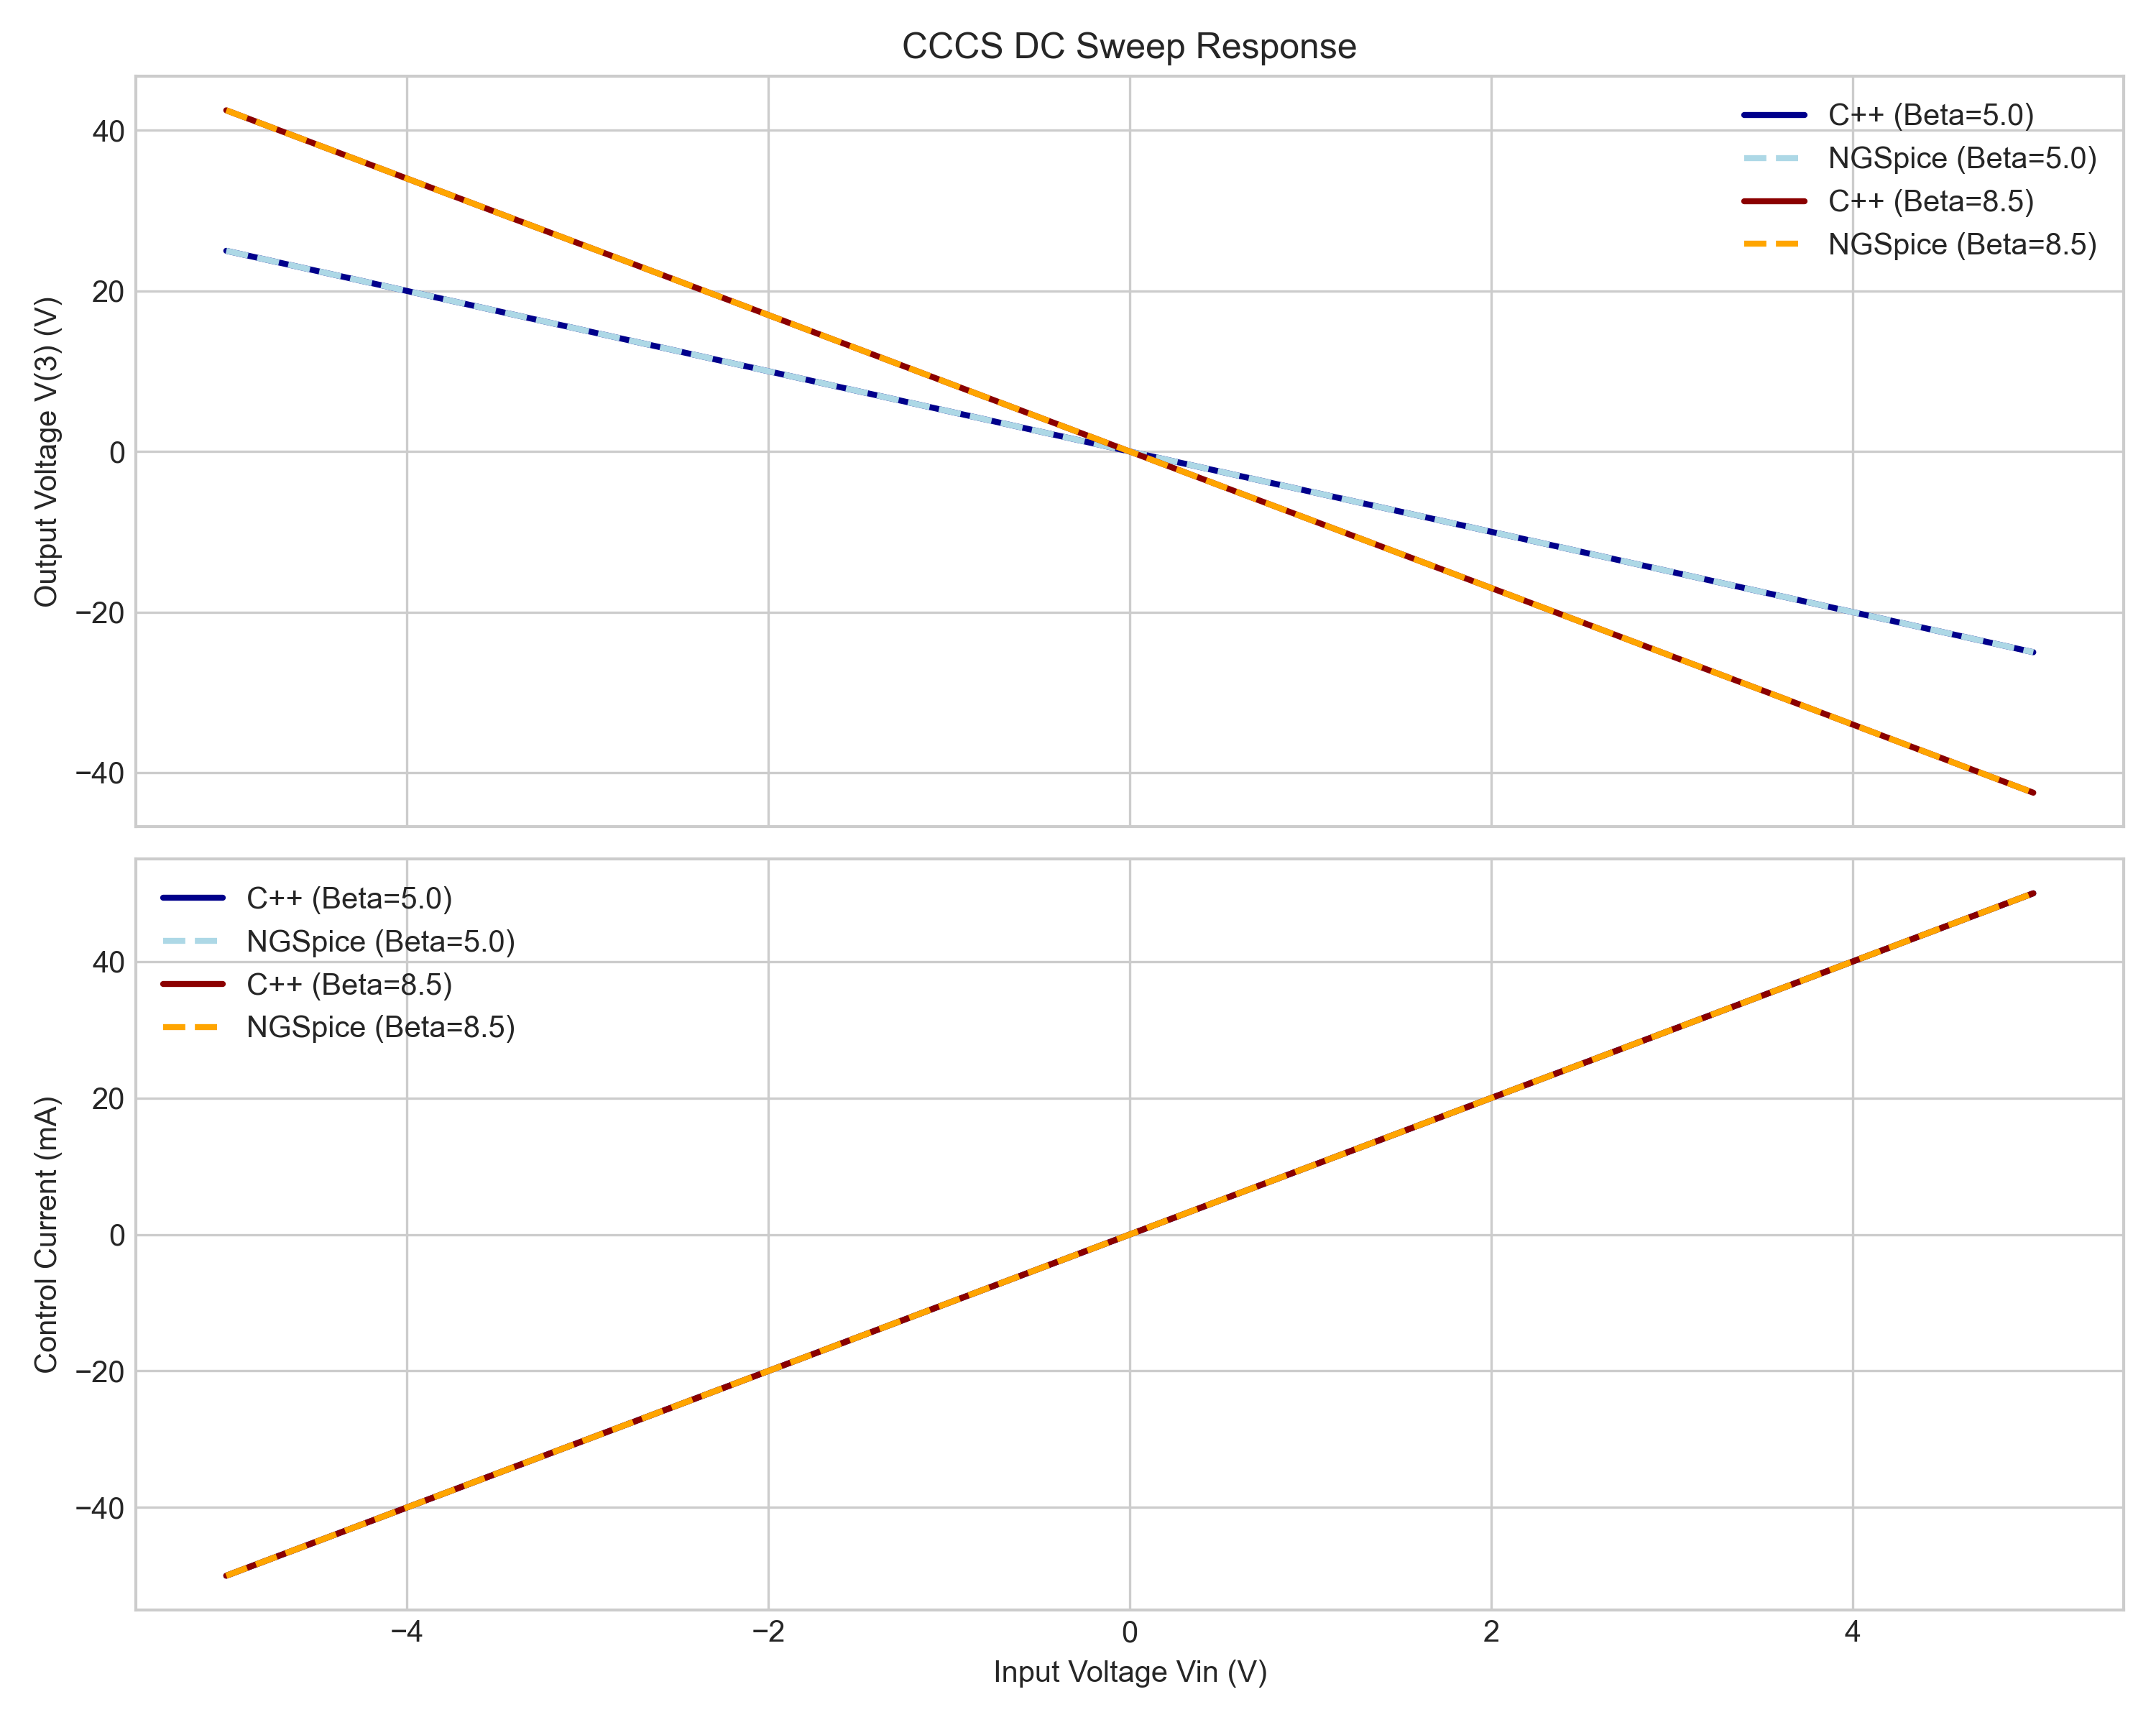
\includegraphics[width=\linewidth]{Figures/Ch5/cccs_4.png}
        \caption{CCCS Current Transfer Test 4.}
        \label{fig:cccs_test_4}
    \end{minipage}
\end{figure}

\begin{figure}[H]
    \centering
    \begin{minipage}{0.48\textwidth}
        \centering
        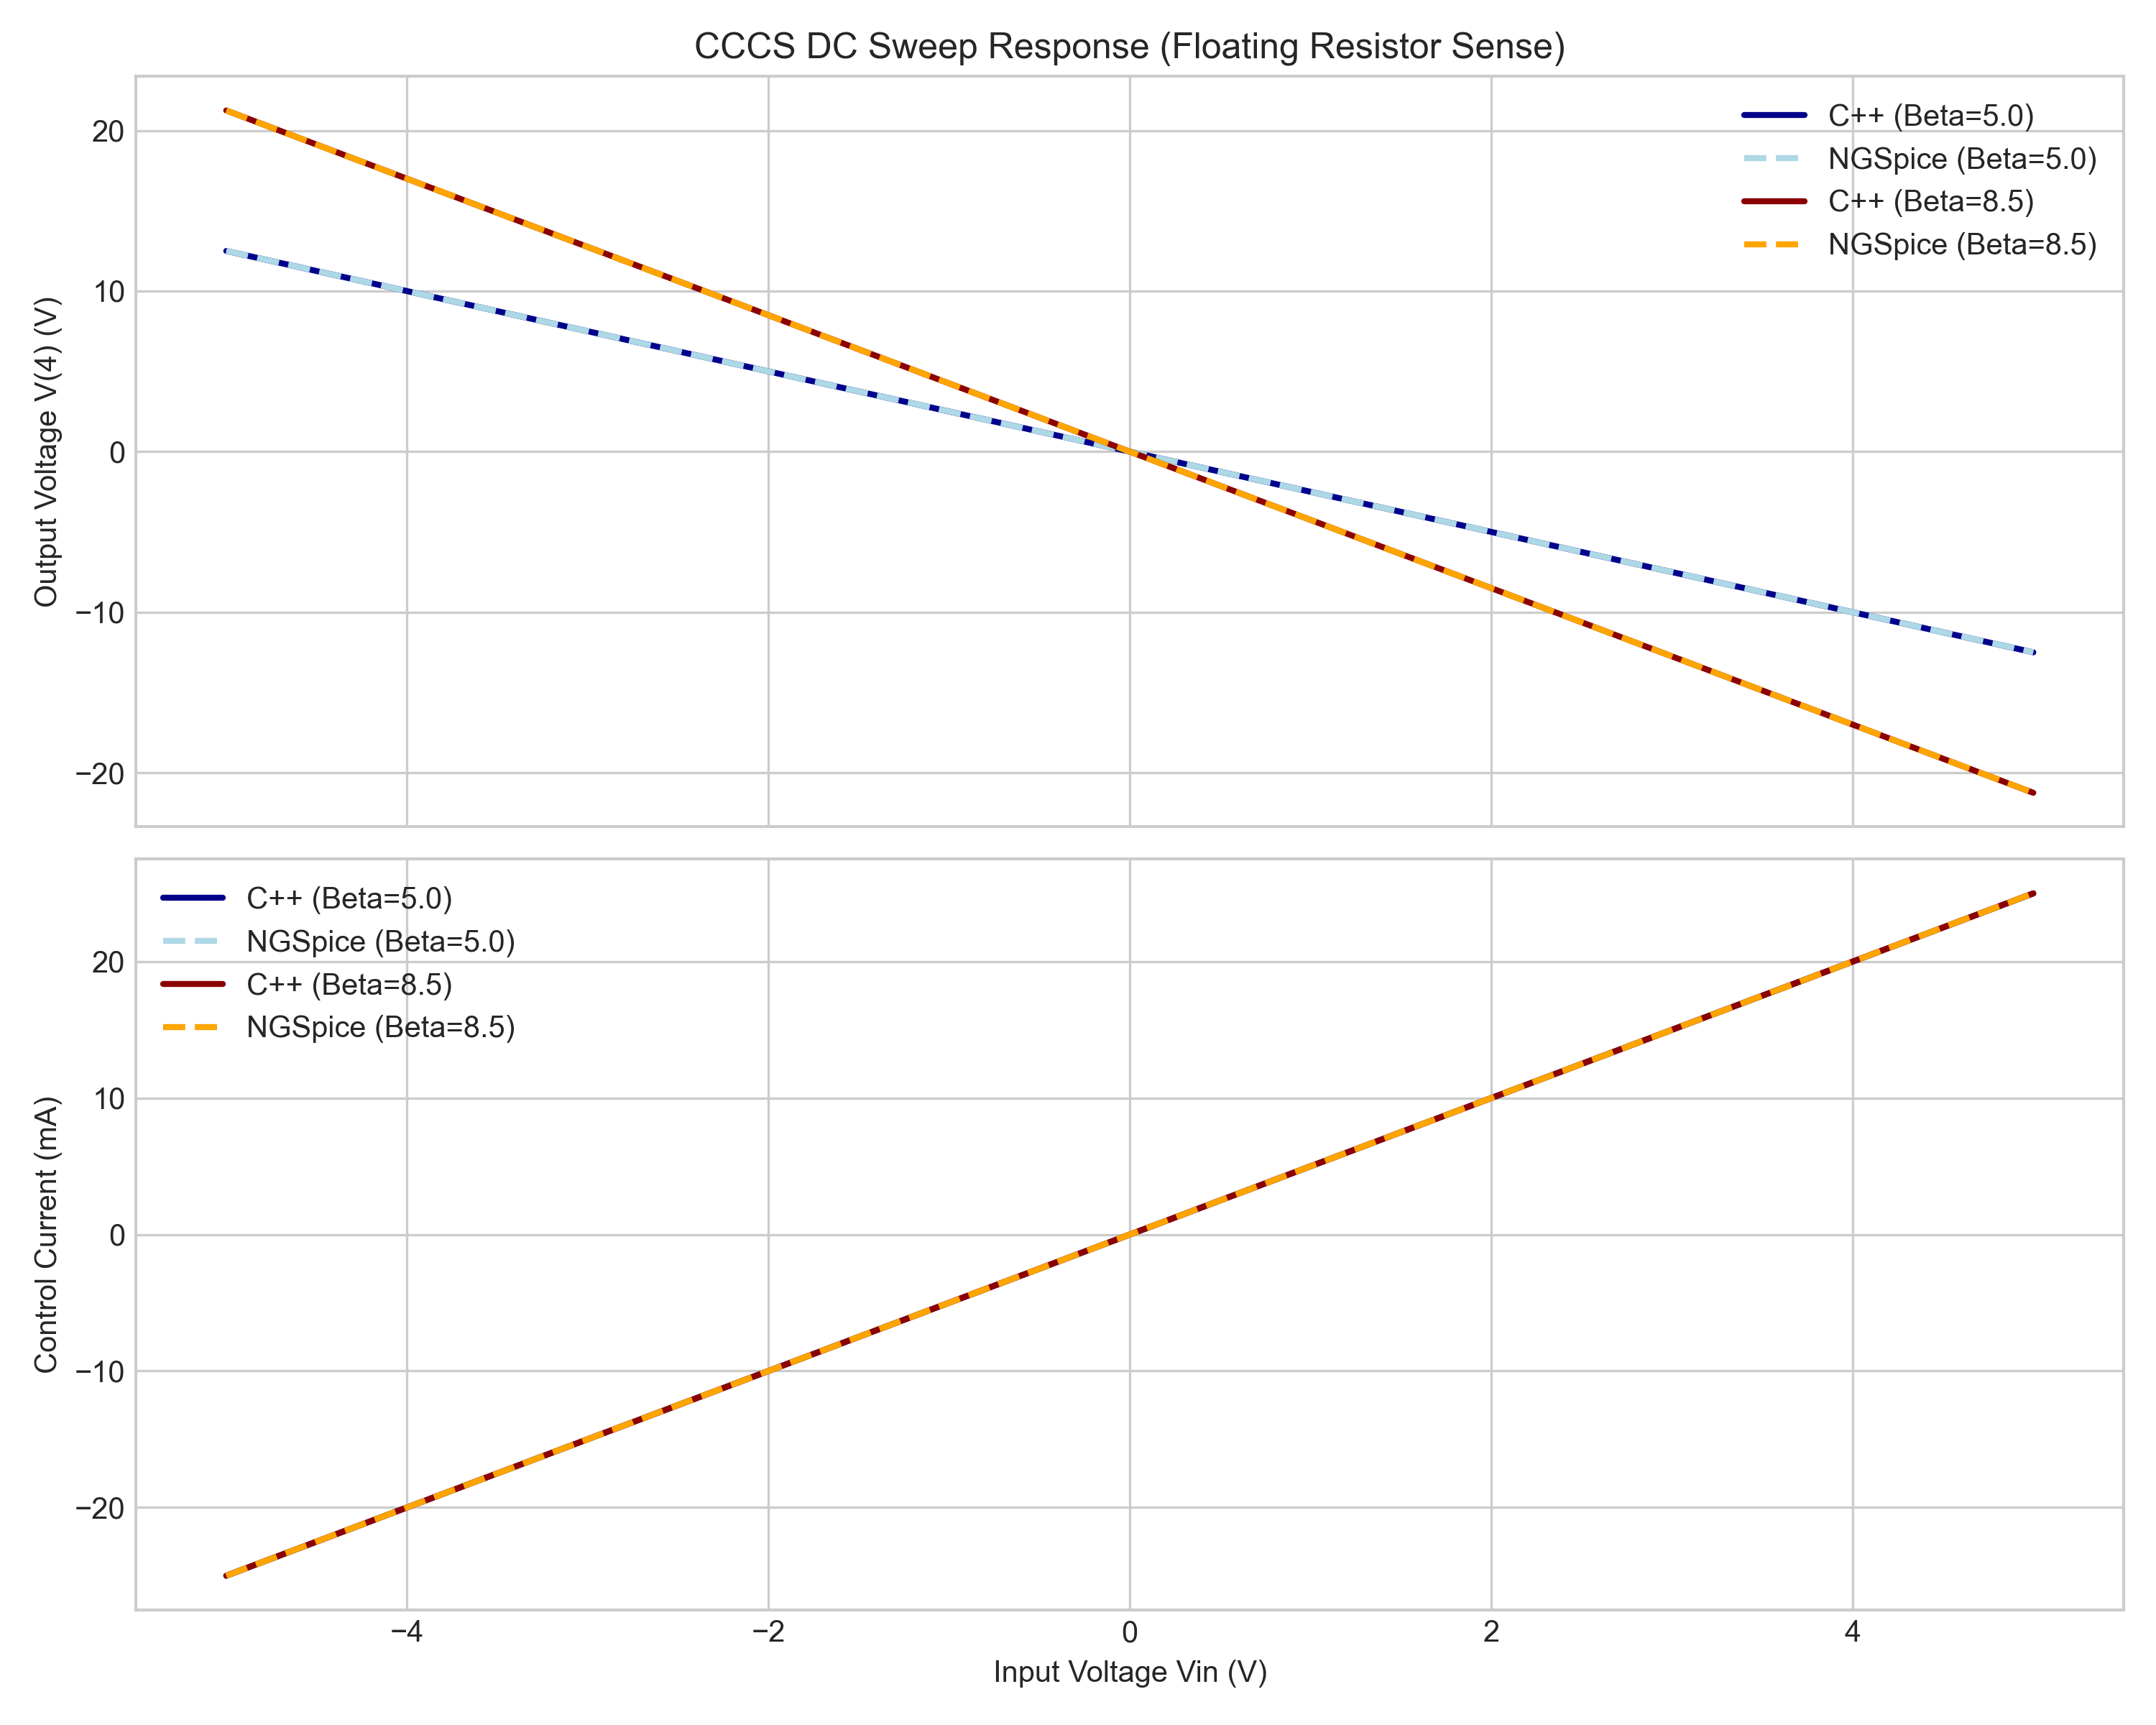
\includegraphics[width=\linewidth]{Figures/Ch5/cccs_5.png}
        \caption{CCCS Current Transfer Test 5.}
        \label{fig:cccs_test_5}
    \end{minipage}\hfill
    \begin{minipage}{0.48\textwidth}
        \centering
        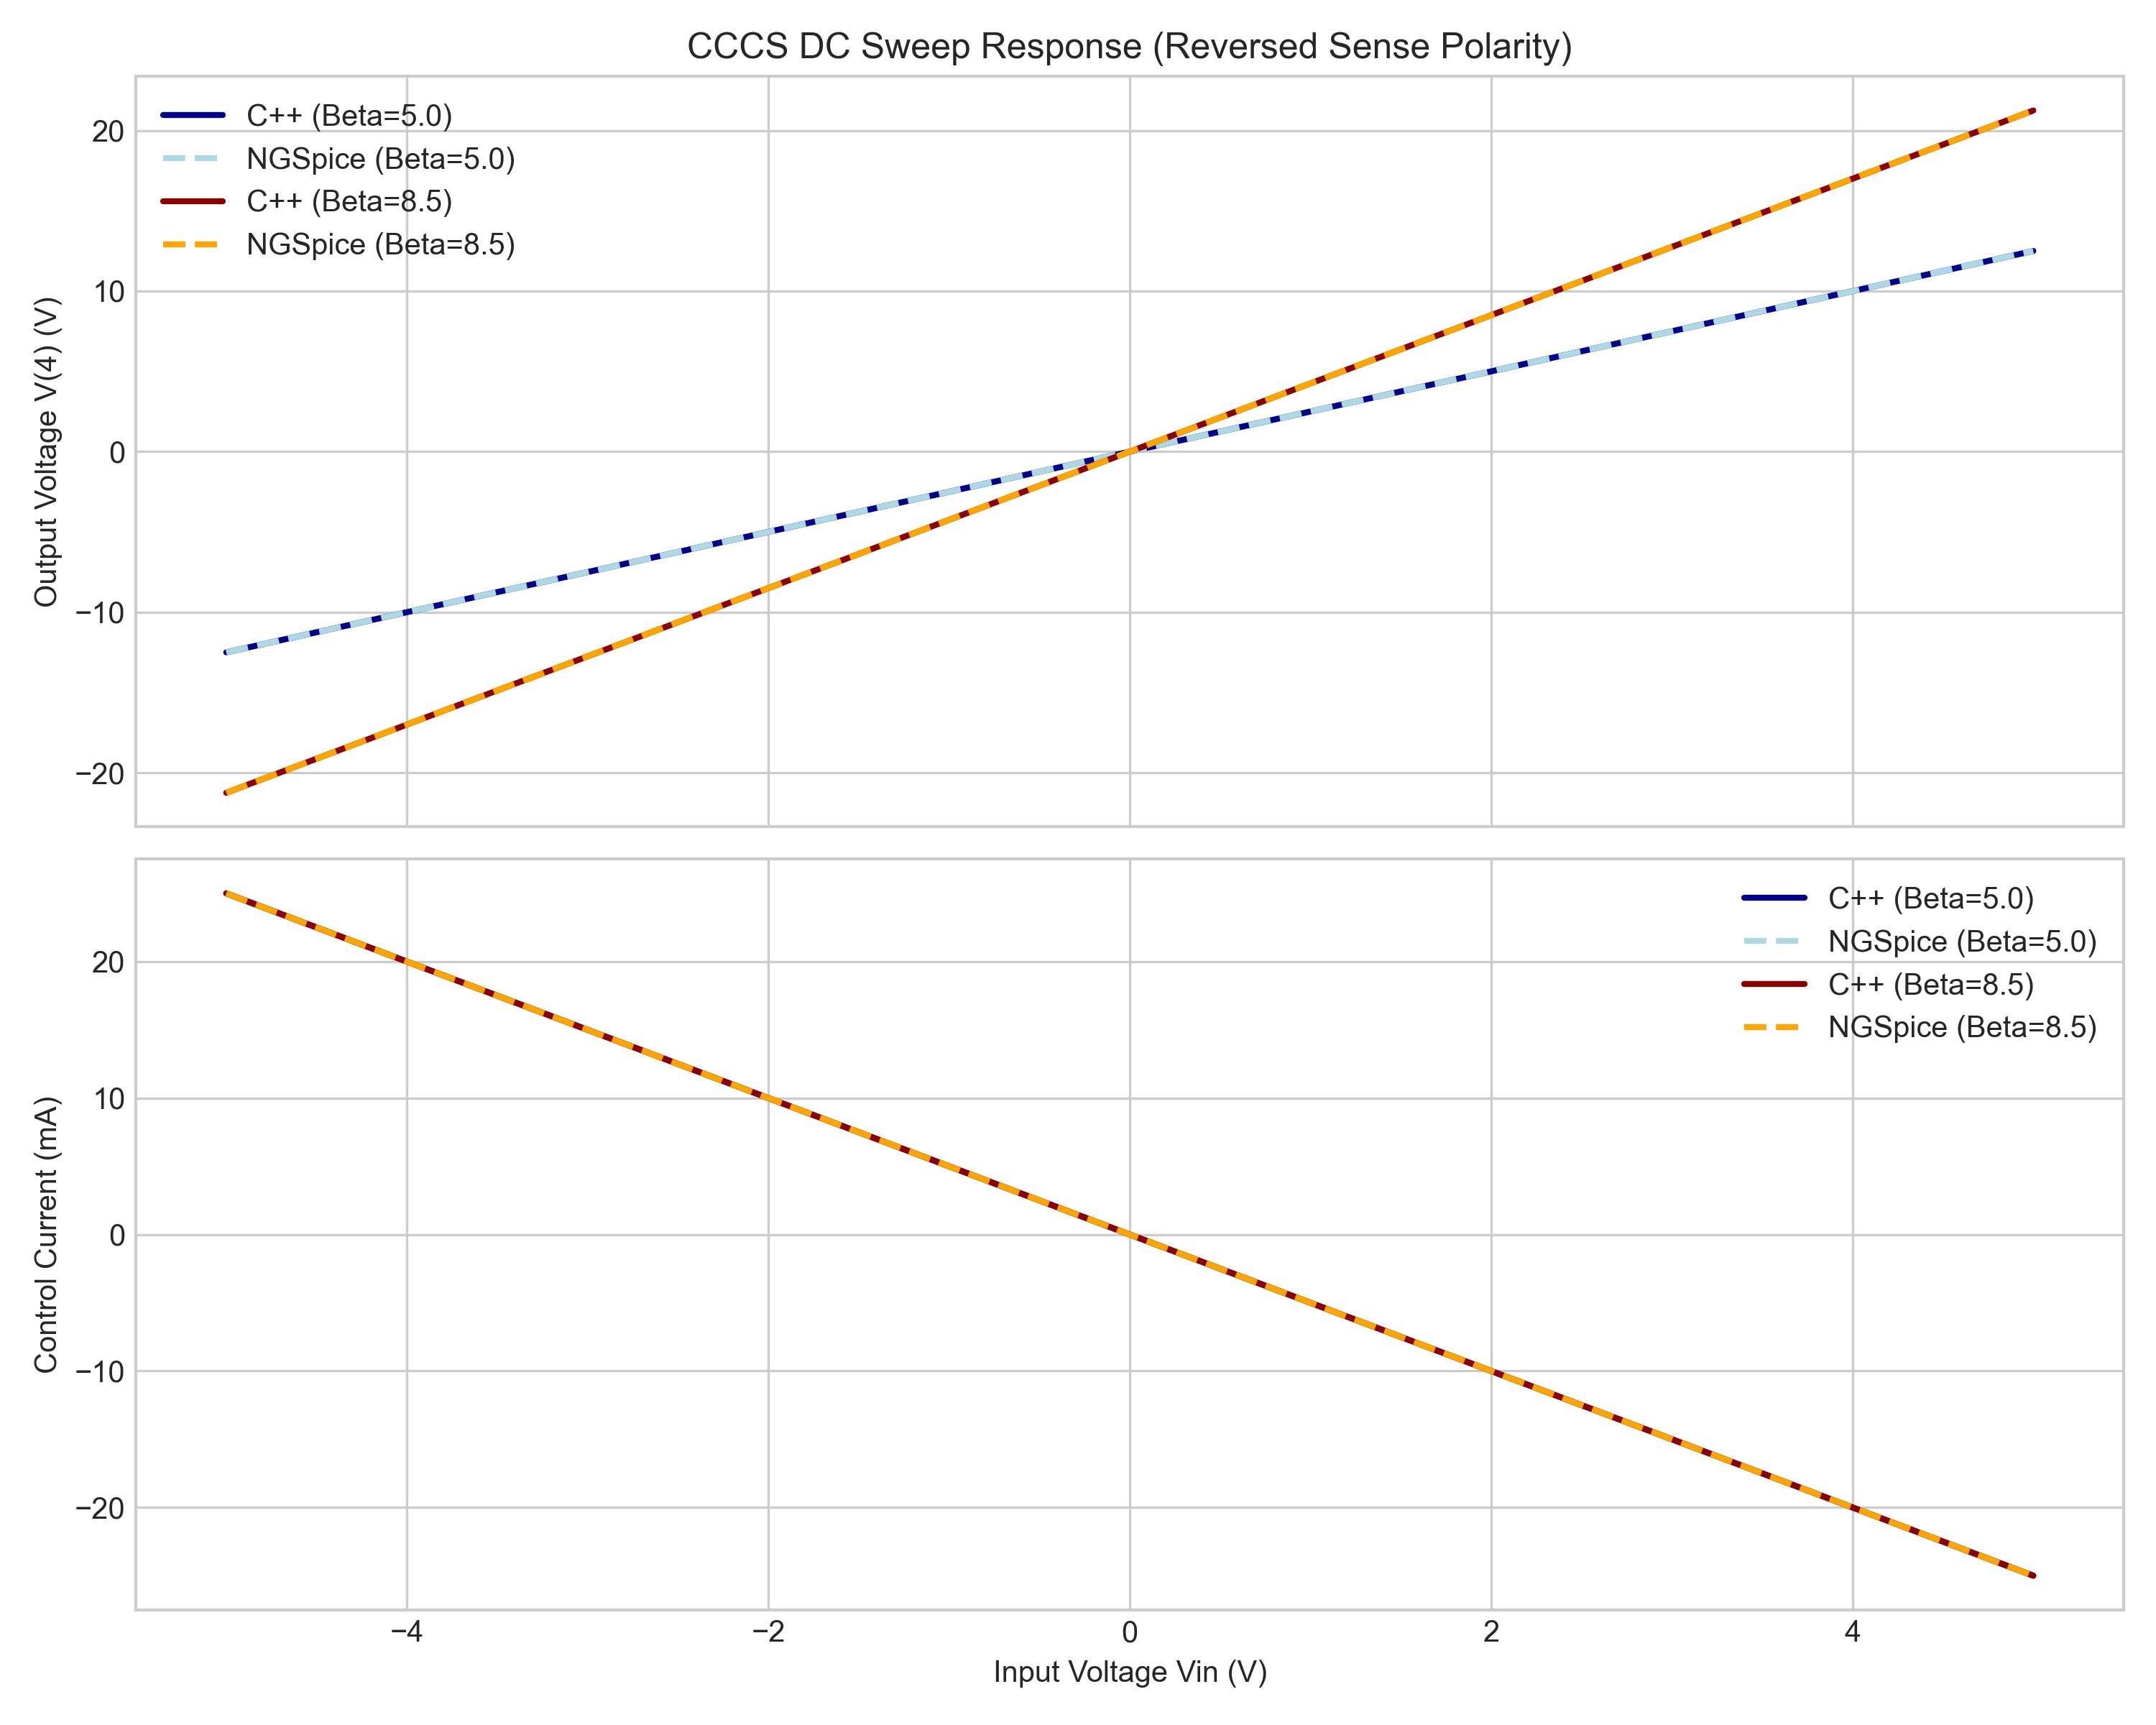
\includegraphics[width=\linewidth]{Figures/Ch5/cccs_6.png}
        \caption{CCCS Current Transfer Test 6.}
        \label{fig:cccs_test_6}
    \end{minipage}
\end{figure}

\subsection{Current-Controlled Voltage Source (CCVS)}
The CCVS tests check transresistance coupling and dual branch current systems.

\subsubsection{Internal C++ Unit Tests}
The C++ testing framework validates the CCVS through an integrated matrix solver sweep:
\begin{itemize}
    \item \textbf{Transresistance Transfer Equation:} Confirms that the output voltage tracks the transresistance multiplier ($H$) times the sensing branch current.
    \item \textbf{MNA Dual-Branch Layout:} Verifies the injection of a new auxiliary branch for the voltage source output, alongside reading the current from a separate existing sensor branch, heavily exercising the MNA dimension scaling.
    \item \textbf{Linear Sweep Simulation:} Sweeps an external source and directly solves the expanded conductance matrix via Gaussian elimination to track dependent branch currents and node voltages.
\end{itemize}

\subsubsection{NGSpice Verification}
Figures~\ref{fig:ccvs_test_1} to \ref{fig:ccvs_test_6} illustrate the NGSpice verification plots for the CCVS transresistance outputs. The output node voltages and source currents demonstrate near-perfect numerical parity with NGSpice across extreme loading scenarios.

\begin{figure}[H]
    \centering
    \begin{minipage}{0.48\textwidth}
        \centering
        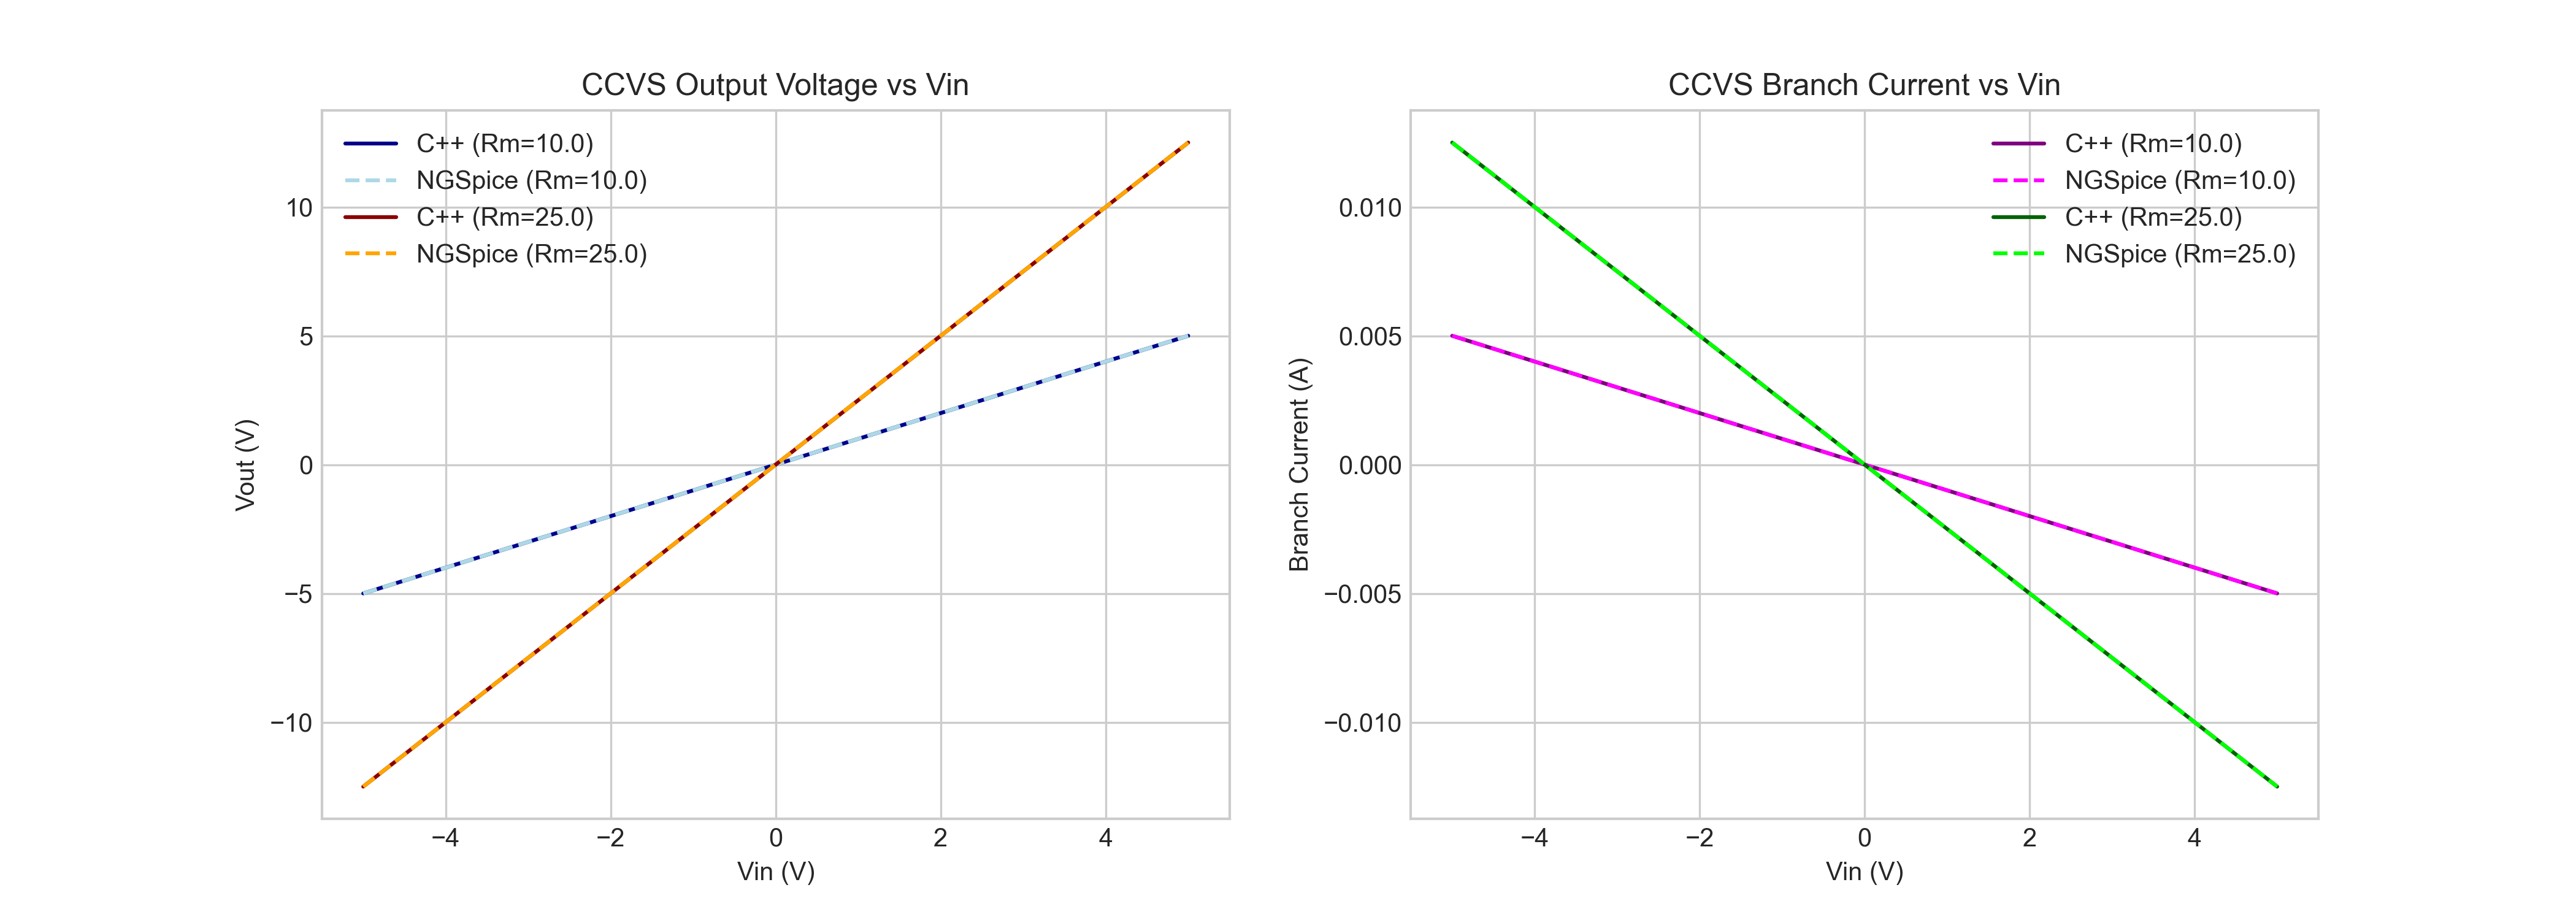
\includegraphics[width=\linewidth]{Figures/Ch5/ccvs_1.png}
        \caption{CCVS Transresistance Test 1.}
        \label{fig:ccvs_test_1}
    \end{minipage}\hfill
    \begin{minipage}{0.48\textwidth}
        \centering
        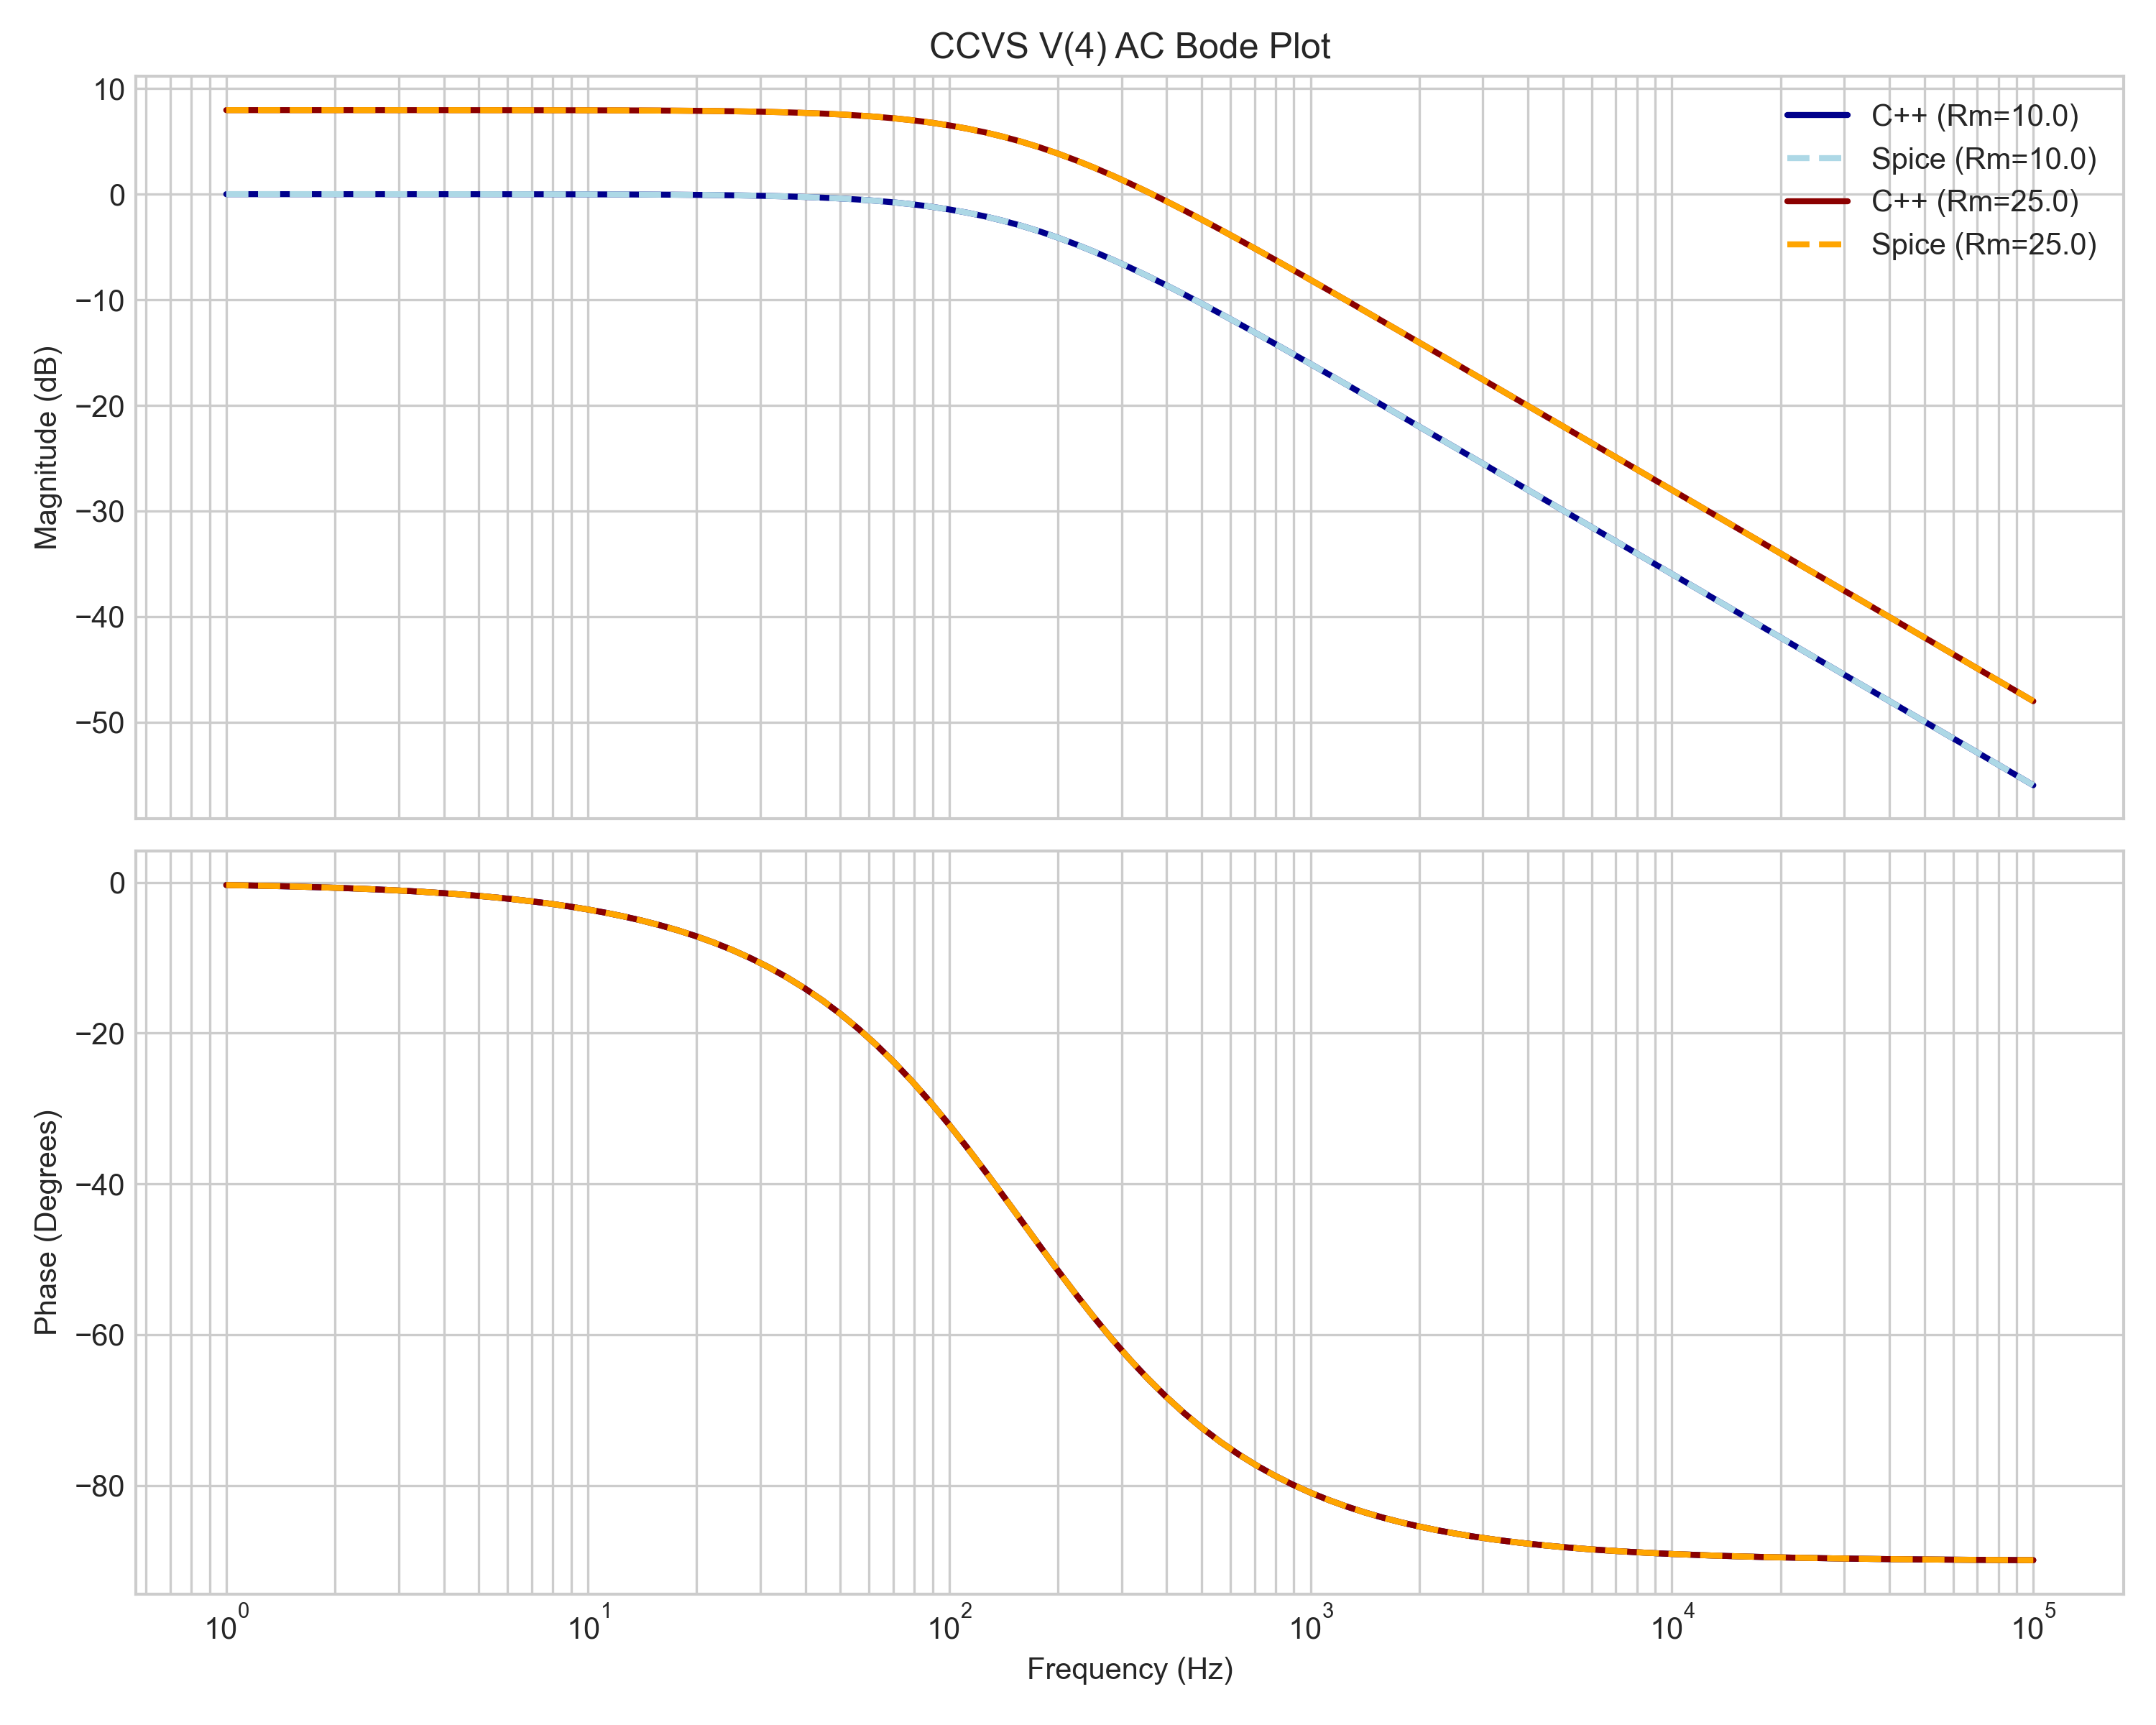
\includegraphics[width=\linewidth]{Figures/Ch5/ccvs_2.png}
        \caption{CCVS Transresistance Test 2.}
        \label{fig:ccvs_test_2}
    \end{minipage}
\end{figure}

\begin{figure}[H]
    \centering
    \begin{minipage}{0.48\textwidth}
        \centering
        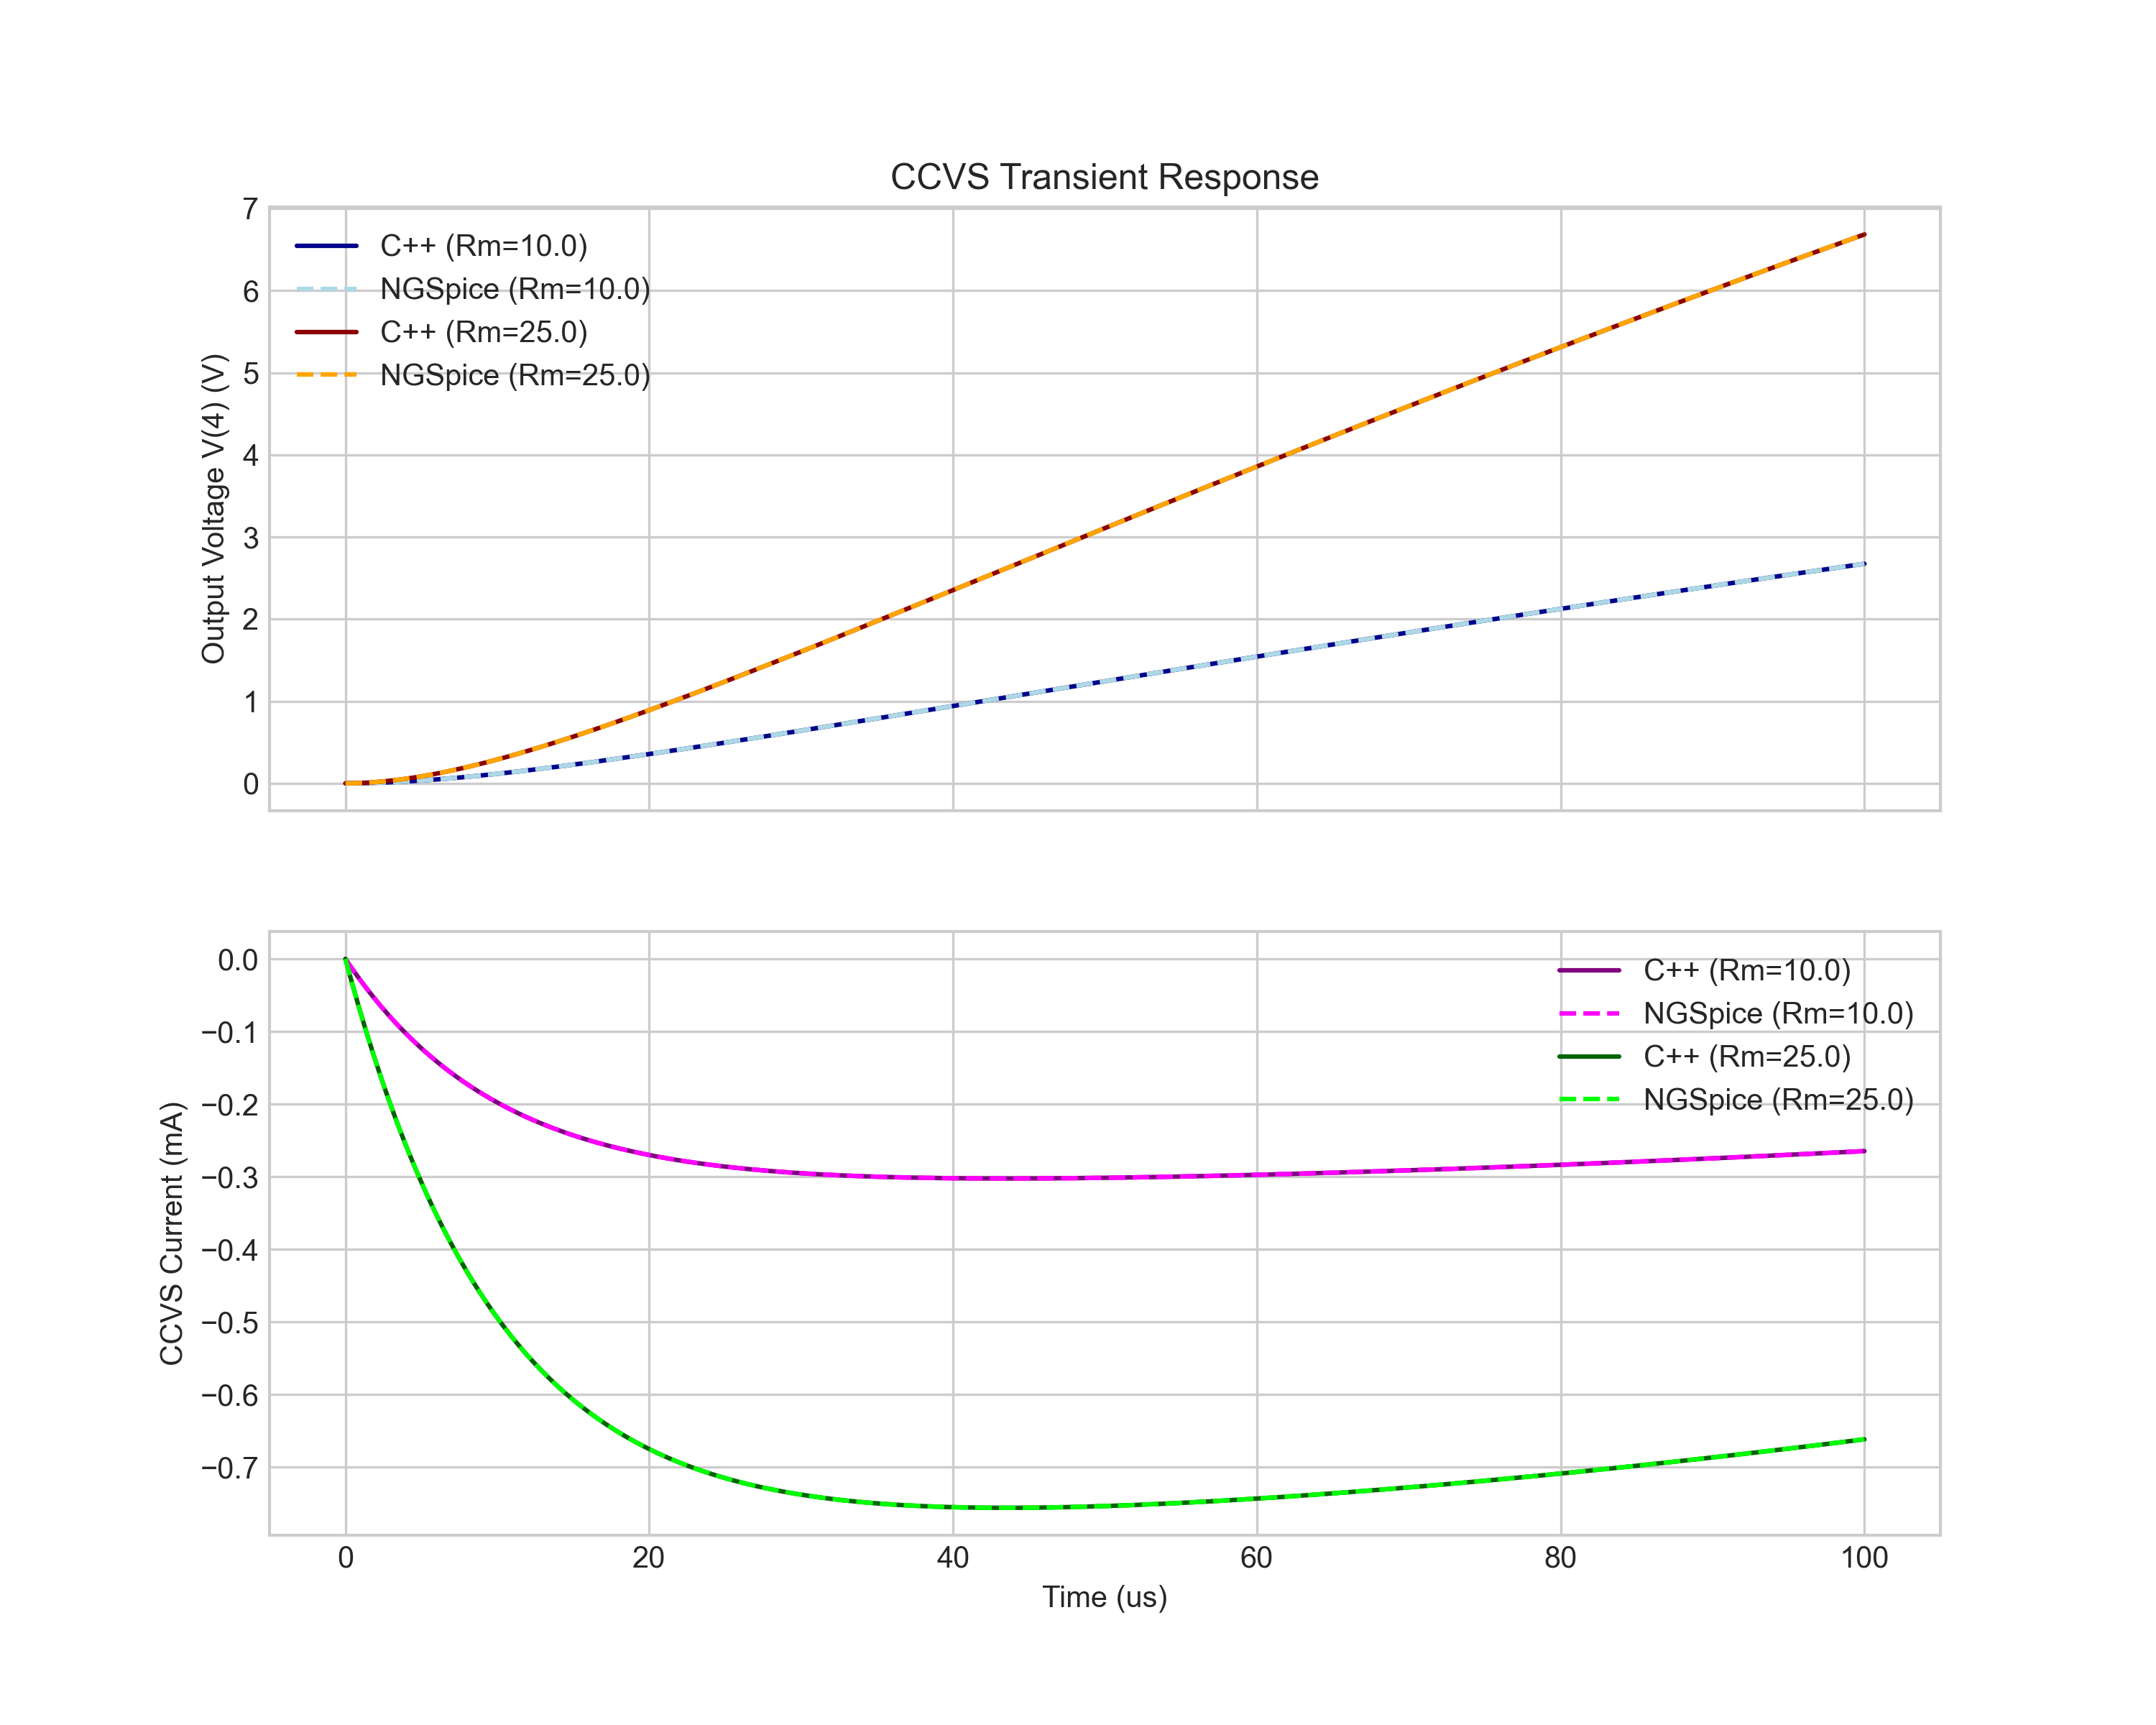
\includegraphics[width=\linewidth]{Figures/Ch5/ccvs_3.png}
        \caption{CCVS Transresistance Test 3.}
        \label{fig:ccvs_test_3}
    \end{minipage}\hfill
    \begin{minipage}{0.48\textwidth}
        \centering
        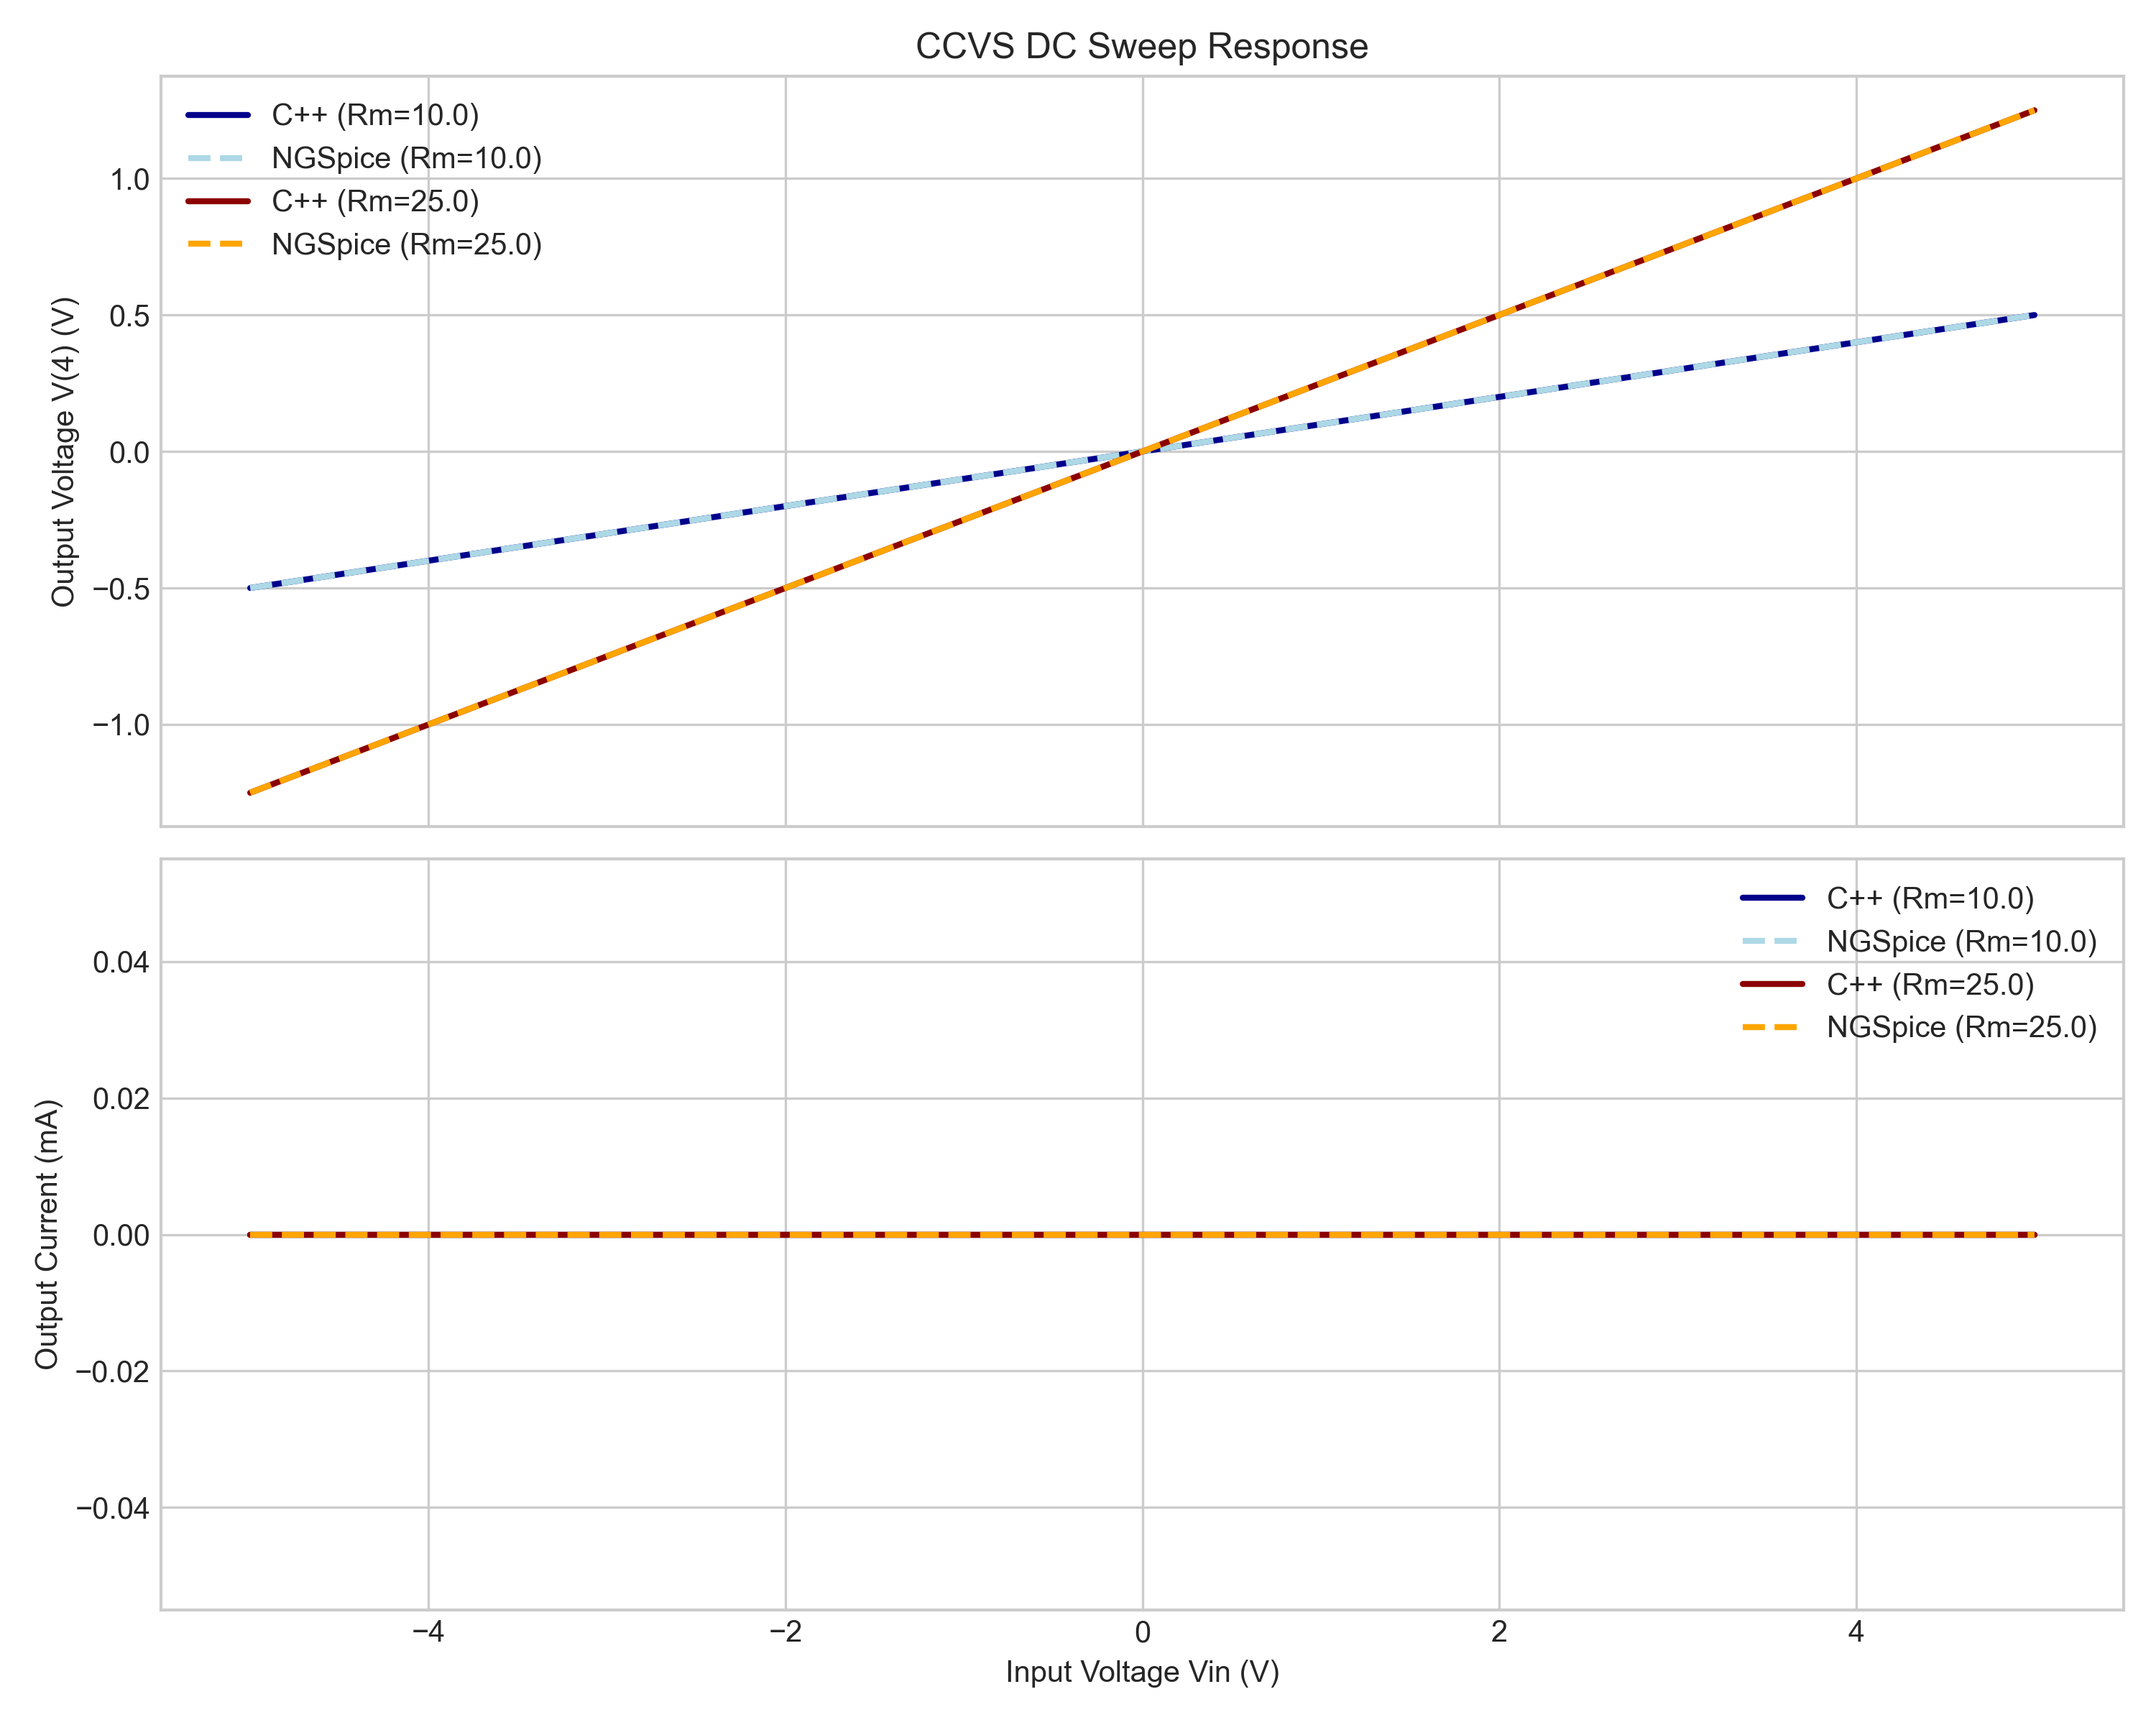
\includegraphics[width=\linewidth]{Figures/Ch5/ccvs_4.png}
        \caption{CCVS Transresistance Test 4.}
        \label{fig:ccvs_test_4}
    \end{minipage}
\end{figure}

\begin{figure}[H]
    \centering
    \begin{minipage}{0.48\textwidth}
        \centering
        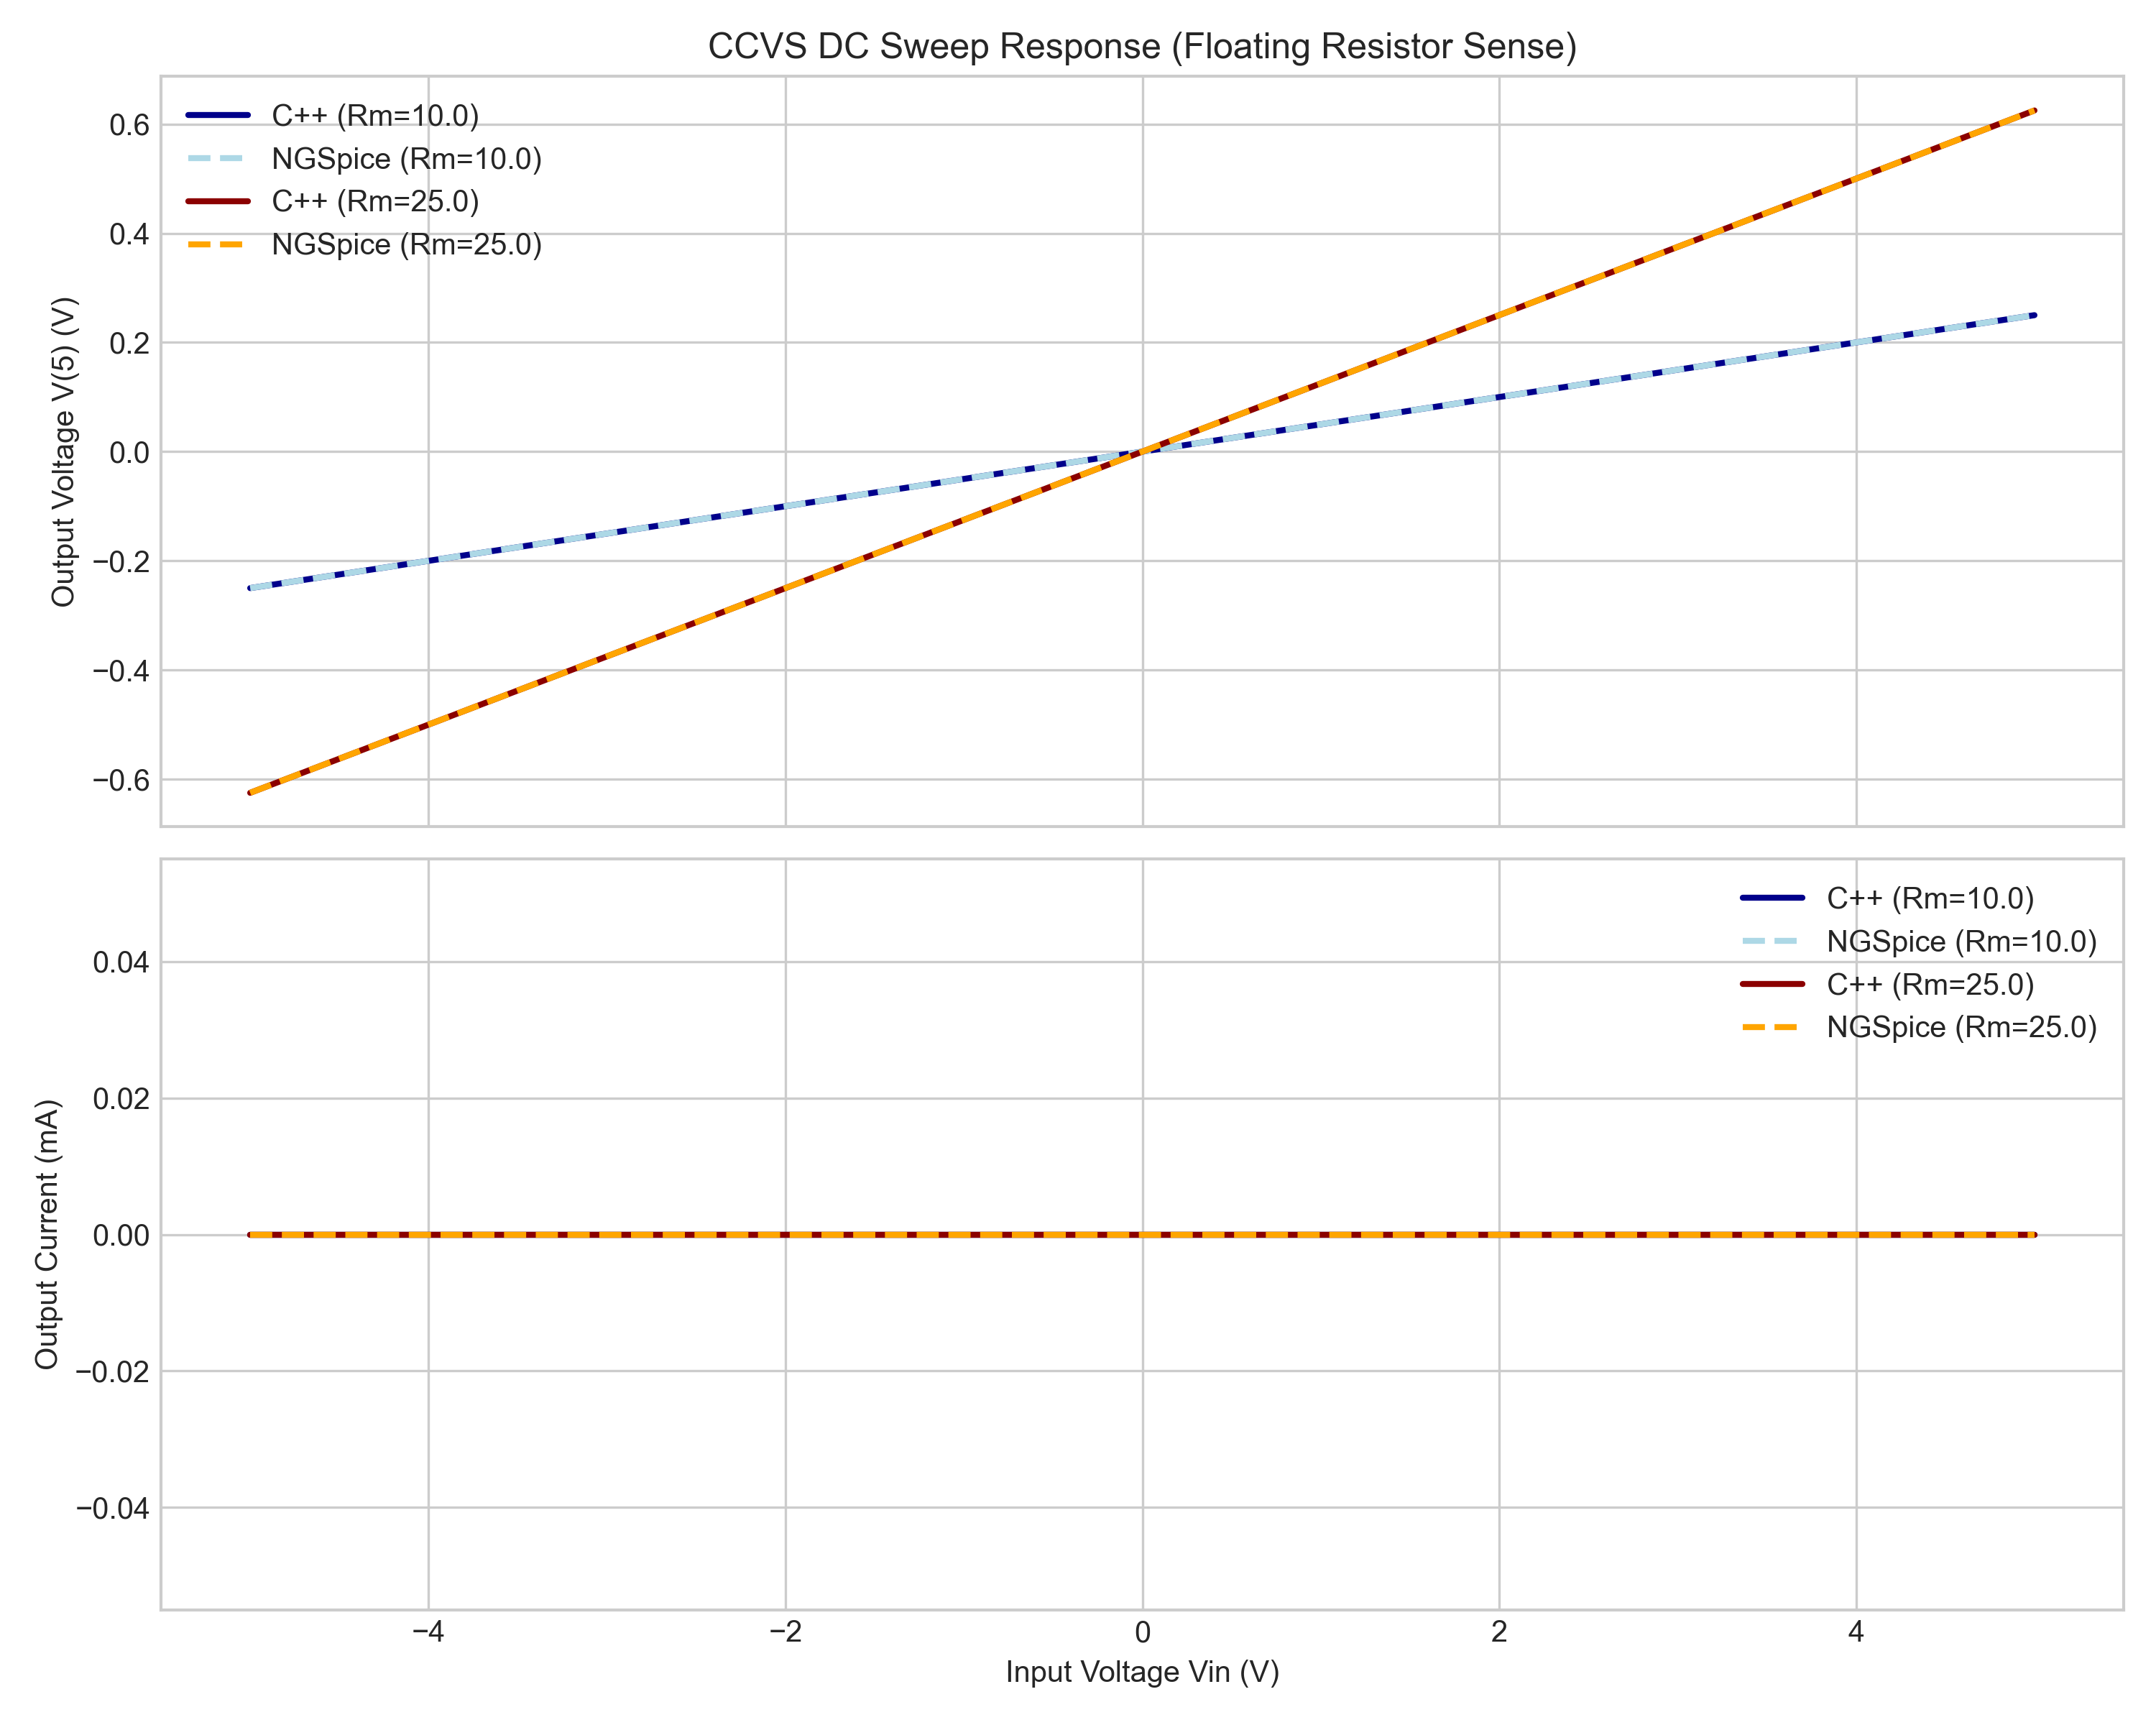
\includegraphics[width=\linewidth]{Figures/Ch5/ccvs_5.png}
        \caption{CCVS Transresistance Test 5.}
        \label{fig:ccvs_test_5}
    \end{minipage}\hfill
    \begin{minipage}{0.48\textwidth}
        \centering
        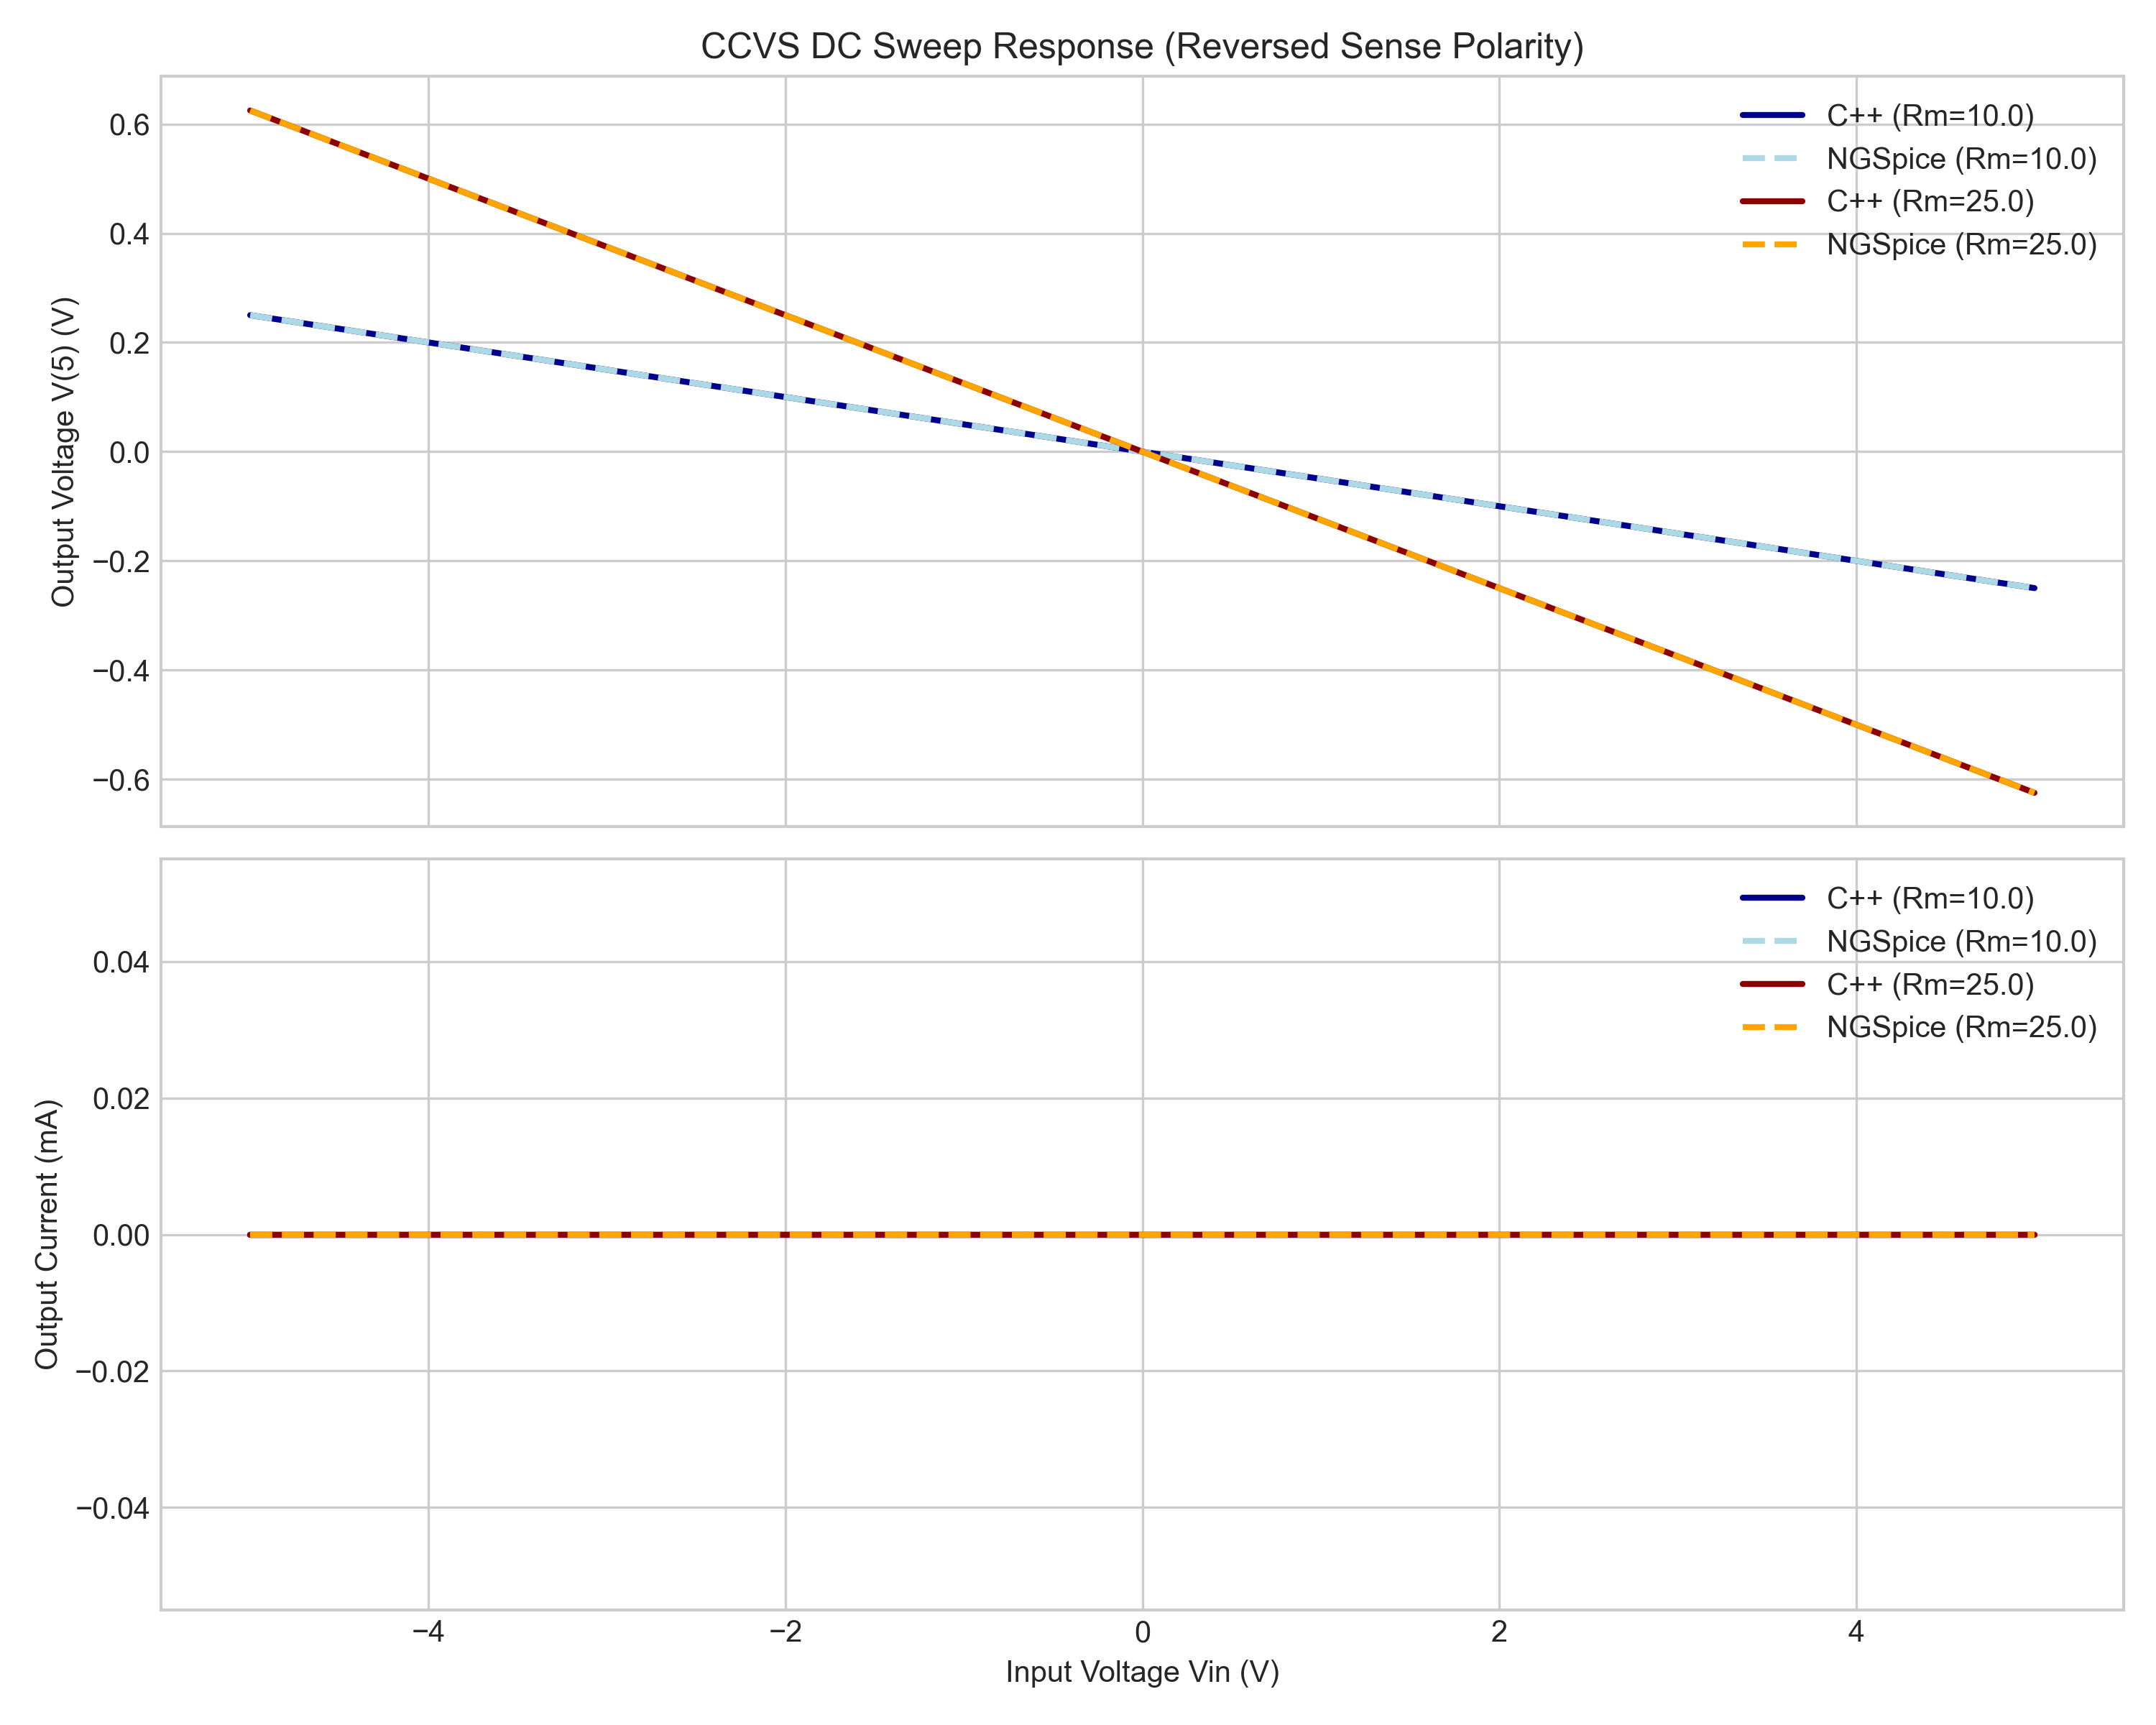
\includegraphics[width=\linewidth]{Figures/Ch5/ccvs_6.png}
        \caption{CCVS Transresistance Test 6.}
        \label{fig:ccvs_test_6}
    \end{minipage}
\end{figure}
